\documentclass{article}
 
\usepackage{authblk}
\usepackage{oldgerm}
\usepackage{mathpartir}
\usepackage{calc}
\usepackage{kpfonts}
\usepackage{esvect}
\usepackage{mathtools}
\usepackage{enumerate}
\usepackage[a4paper]{geometry}
\usepackage{url}
\usepackage[english]{babel}
\usepackage[utf8]{inputenc}
\usepackage{amsmath,amsfonts,amsthm,stmaryrd}
\usepackage{thmtools}
\usepackage[bookmarks,
            pagebackref,
            colorlinks,
            linkcolor={red!50!black},
            citecolor={blue!50!black},
            urlcolor={blue!80!black}]{hyperref}

\hypersetup{
  pdfauthor={Lars Birkedal and Ale\v{s} Bizjak},
  pdftitle={Lecture Notes on Iris: Higher-Order Concurrent Separation Logic}
}

\usepackage[usenames,dvipsnames]{xcolor}

\usepackage{pftools}

% iris specific macros
\usepackage{iris}
\usepackage{heaplang}

\usepackage{tikz}
\usepackage{tikz-cd}

\usepackage{verbatim}

\usepackage{calc}
\usetikzlibrary{positioning}
\usetikzlibrary{decorations.pathreplacing}

\newenvironment{invdrawing}{
  \begin{tikzpicture}
    \tikzstyle{nn} = [inner sep=0pt,outer sep=0pt, text width=30pt, align=center, text height=15pt]
    \tikzstyle{braceunder} = [decoration={brace,amplitude=10pt,mirror,raise=2pt},decorate,thick]
    \tikzstyle{braceover} = [decoration={brace,amplitude=10pt,raise=2pt},decorate,thick]
    \colorlet{c1}{olive!50}
    \colorlet{c2}{red!70}
    \colorlet{c3}{blue!40}
  }
  {\end{tikzpicture}}

\declaretheorem[style=plain,numberwithin=section]{theorem}
\declaretheorem[style=plain,sibling=theorem]{lemma}
\declaretheorem[style=plain,sibling=theorem]{proposition}
\declaretheorem[style=plain,sibling=theorem]{corollary}

\declaretheorem[style=definition,qed=$\blacksquare$,sibling=theorem]{definition}
\declaretheorem[style=definition,qed=$\blacksquare$,sibling=theorem]{example}
\declaretheorem[style=definition,qed=$\blacksquare$,sibling=theorem]{remark}
\declaretheorem[style=definition,qed=$\diamondsuit$,sibling=theorem]{exercise}


\renewcommand{\implies}{\Rightarrow}
\newcommand{\kleeneeq}{\ensuremath{\simeq}}
\newcommand{\partfun}{\ensuremath{\rightharpoonup}}
\newcommand{\finparmap}{\overset{\text{fin}}{\rightharpoonup}}
\newcommand{\id}[1]{\ensuremath{\text{id}_{#1}}}
\newcommand{\NN}{\ensuremath{\mathbb{N}}}
\newcommand{\QQ}{\ensuremath{\mathbb{Q}}}
\newcommand{\RR}{\ensuremath{\mathbb{R}}}
\newcommand{\HH}{\ensuremath{\mathbb{H}}}
\newcommand{\seqn}[1]{\ensuremath{\left(#1\right)_{n=0}^{\infty}}}
\newcommand{\seqns}[1]{\ensuremath{\left\{#1\right\}_{n=0}^{\infty}}}
\newcommand{\sequen}[3]{\ensuremath{{#1 \isetsep #2 \vdash #3}}}
\newcommand{\hastype}[3]{\ensuremath{{#1 \vdash #2 : #3}}}
\newcommand{\closure}[1]{\ensuremath{\text{Cl}\left(#1\right)}}

\newcommand{\timelessjudg}[1]{\proves #1\ \textlog{timeless}}

% semantics
\newcommand{\den}[1]{\ensuremath{\left\llbracket #1 \right\rrbracket}}
\newcommand{\nequal}[1]{\ensuremath{\overset{#1}{=}}}
\newcommand{\cut}[2]{\ensuremath{\left\lfloor #2 \right\rfloor_{#1}}}

\renewcommand{\phi}{\varphi}
\renewcommand{\theta}{\vartheta}
\newcommand{\eps}{\varepsilon}
\renewcommand{\epsilon}{\varepsilon}

\renewcommand{\hom}[3]{\ensuremath{\text{Hom}_{#1}\left(#2,#3\right)}}
\newcommand{\iso}{\cong}
\newcommand{\riso}{\overset{\approx}{\rightarrow}}

\newenvironment{diagram}{\begin{tikzcd}[row sep=1.5cm,column sep=1.5cm]}{\end{tikzcd}}
\newenvironment{largediagram}{\begin{tikzcd}[row sep=2.6cm,column sep=2.6cm]}{\end{tikzcd}}
\newenvironment{smalldiagram}{\begin{tikzcd}[row sep=1cm,column sep=1cm]}{\end{tikzcd}}

% various categories
\newcommand{\CAT}{\ensuremath{\mathbf{Cat}}}
\newcommand{\sets}{\ensuremath{\mathbf{Set}}}
\newcommand{\heyt}{\ensuremath{\mathbf{Heyt}}}
\newcommand{\PSh}[1]{\ensuremath{\text{PSh}\left(#1\right)}}
\newcommand{\subobj}[1]{\ensuremath{\mathbf{Sub}\left(#1\right)}}
\newcommand{\subobjf}[2]{\ensuremath{\mathbf{Sub}_{#1}\left(#2\right)}}

\newcommand{\BB}{\ensuremath{\mathbb{B}}}
\newcommand{\Cc}{\ensuremath{\mathbf{C}}}
\newcommand{\El}{\ensuremath{\mathcal{E}}}
\newcommand{\Sl}{\ensuremath{\mathcal{S}}}
\newcommand{\Ul}{\ensuremath{\mathcal{U}}}
\newcommand{\Dl}{\ensuremath{\mathcal{D}}}
\newcommand{\Fl}{\ensuremath{\mathcal{F}}}
\newcommand{\Pl}{\ensuremath{\mathcal{P}}}
\newcommand{\Tl}{\ensuremath{\mathcal{T}}}
\newcommand{\CC}{\ensuremath{\mathbb{C}}}
\newcommand{\KK}{\ensuremath{\mathbb{K}}}
\newcommand{\PP}{\ensuremath{\mathbb{P}}}
\newcommand{\VV}{\ensuremath{\mathbb{V}}}
\newcommand{\UU}{\ensuremath{\mathbb{U}}}
\newcommand{\DD}{\ensuremath{\mathbb{D}}}
\newcommand{\Ml}{\ensuremath{\mathcal{M}}}
\newcommand{\Vl}{\ensuremath{\mathcal{V}}}
\newcommand{\Il}{\ensuremath{\mathcal{I}}}
\newcommand{\Cl}{\ensuremath{\mathcal{C}}}
\newcommand{\Bl}{\ensuremath{\mathcal{B}}}
\newcommand{\Al}{\ensuremath{\mathcal{A}}}
\newcommand{\Gl}{\ensuremath{\mathcal{G}}}
\newcommand{\Nl}{\ensuremath{\mathcal{N}}}
\newcommand{\AAA}{\ensuremath{\mathbb{A}}}
\newcommand{\EE}{\ensuremath{\mathbb{E}}}

% separators
\newcommand{\isetsep}{\;\ifnum\currentgrouptype=16 \middle\fi|\;}

% other notations
\newcommand{\powerset}[1]{\ensuremath{\mathcal{P}\left(#1\right)}}
\newcommand{\upred}[1]{\ensuremath{\mathbf{UPred}\left(#1\right)}}
\newcommand{\powup}[1]{\ensuremath{\mathcal{P}^{\uparrow}\left(#1\right)}}
\newcommand{\powdown}[1]{\ensuremath{\mathcal{P}^{\downarrow}\left(#1\right)}}
\newcommand{\restr}[2]{\ensuremath{\mathbf{r}_{#2}^{#1}}}
\newcommand{\reindex}[1]{\ensuremath{#1^*}}
\newcommand{\limit}{\varprojlim}
\newcommand{\colimit}{\varinjlim}
\newcommand{\blackbox}{\blacksquare}
\newcommand{\blackdiamond}{\blacklozenge}

% text macros
\newcommand{\ie}{\emph{i.e.,}}
\newcommand{\eg}{\emph{e.g.,}}
\newcommand{\etc}{\emph{etc.}}


% programming language
\newcommand{\proglang}{$\lambda_{\mathrm{ref},\mathrm{conc}}$}
% basic steps of the operational semantics
\newcommand{\stepstopure}{\overset{\mathrm{pure}}{\rightsquigarrow}}
\newcommand{\stepsto}{\rightsquigarrow}
% One-step reduction of thread pools (configurations)
\newcommand{\cstepsto}{\rightarrow}

\newcommand{\Heap}{\textdom{Heap}}
\newcommand{\ECtx}{\textdom{ECtx}}
\newcommand{\TPool}{\textdom{TPool}}
\newcommand{\Config}{\textdom{Config}}

\newcommand{\inl}{\operatorname{inl}}
\newcommand{\inr}{\operatorname{inr}}
\newcommand{\case}[5]{\operatorname{case}(#1,#2.#3,#4.#5)}

% parallel composition operator
\newcommand{\parcomp}{\ensuremath{\mathbin{||}}}

\newcommand{\freevars}[1]{\ensuremath{\text{FV}\left(#1\right)}}

\newcommand{\Iris}{Iris}
\newcommand{\Coq}{Coq}

%% Macros for constructing iterated inference rules with similar labels
% Constructs a rule with name #2, label #3 (with postfix #1; default empty),
% hypotheses #4 and conclusion #5
% ex: \rulegenhref[-app]{$\ast$-weak}{star-weak}{ }{P_1 \ast P_2 \proves P_1}
\newcommand{\rulegenhref}[5][]{\inferhref{#2}{#3#1}{#4}{#5}}
% Variant for constructing bi-inference rules
\newcommand{\rulegenhrefb}[5][]{\inferhrefB{#2}{#3#1}{#4}{#5}}
% Variant where name and label coincide
\newcommand{\rulegen}[4][]{\rulegenhref[#1]{#2}{#2}{#3}{#4}}
% Variant of bi-inference where name and label coincide
\newcommand{\rulegenb}[4][]{\rulegenhrefb[#1]{#2}{#2}{#3}{#4}}

% Hoare post condition ignore-arg blank (_.)
\newcommand{\ignarg}{\_\,.\,}

%% TODO: Upstream these in the iris.sty file
\newcommand{\pointsto}{\mapsto}
\newcommand{\persistently}{\always}

\newcommand{\option}[1]{\maybe{#1}}
\newcommand{\Some}{\operatorname{Some}}
\newcommand{\None}{\operatorname{None}}

% types
\newcommand{\tvar}{X}
\newcommand{\tvarB}{Y}
\newcommand{\TVar}{\textdom{Tvar}}

\newcommand{\typ}{\tau}
\newcommand{\typB}{\rho}
\newcommand{\Tunit}{1}
\newcommand{\Tbool}{\mathbb{B}}
\newcommand{\Tnat}{\mathbb{N}}
\newcommand{\Tarr}{\ra}
\newcommand{\TLam}{\Lambda\spac}
\def\Tall #1.{\forall #1.\spac}%
\def\Tmu #1.{\mu #1.\spac}%
\def\Tref(#1){\textlang{ref}(#1)}

\newcommand{\Tenv}{\Xi}
\newcommand{\env}{\Gamma}
\newcommand{\typed}[4]{#1 ~|~ #2 \vdash #3 : #4}
\newcommand{\semtyped}[4]{#1 ~|~ #2 \vDash #3 : #4}

% logical relations
\newcommand{\semenv}{\Delta}

\renewcommand{\Prop}{\mProp}

% Multiple argument macros with consistent spacing
\newcommand{\twoArgMacro}[2]{\newcommand{#1}[2]{#2 ##1 \spac ##2}}
\twoArgMacro{\isList}{\operatorname{isList}}
\twoArgMacro{\map}{\operatorname{map}}
\twoArgMacro{\listFilter}{\operatorname{listFilter}}
\twoArgMacro{\all}{\operatorname{all}}

%%% Local Variables:
%%% mode: latex
%%% TeX-master: "main"
%%% End:


%%%%%%%%%%%%%%%%%%%%%%%%%%%%%%%%%%%%%%%%%%%%%%%%%%%%%%%%%%%%%%%%
% hoare proof typesetting (from setup.sty)

\usepackage{array}\extrarowheight=\jot	% else, arrays are scrunched compared to, say, aligned
\newcolumntype{.}{@{}}
\usepackage{tabu}
\usepackage{rotating}
\usepackage{xstring}
\usepackage{xspace}
\usepackage{semantic}
\usepackage{csquotes}
\usepackage{cleveref}

\newcommand{\tabubox}[2][]{%
  \begin{tabu}{@{#1}X[1,l,m]@{}}%
    #2 %
  \end{tabu}%
}
\newcommand{\hproofnospace}[1]{\noindent\parbox{\linewidth}{#1}} %
\newcommand{\hproof}[1]{\vspace{0.5em}\hproofnospace{#1}\vspace{0.5em}} %
\newcommand\psub[2]{%
  \begin{tabu}{ m{0.9em} | X[1,l,m] }%
    \begin{sideways}#1\end{sideways} &%
    \tabubox{#2}%
  \end{tabu}%
}%

\newcommand\pind[1]{\tabubox[\hspace{1em}]{#1}}
\newcommand{\mline}[1]{\ensuremath{#1}}
\newcommand{\pline}[2][\empty]{\ensuremath{\left\{{#2\mathstrut}\right\}_{#1}}}
\newcommand{\pmline}[2][\empty]{\ensuremath{\left\{\begin{inbox}#2\end{inbox}\right\}_{#1}}}
\newcommand{\aline}[2][\empty]{\ensuremath{{\stretchleftright[450]{\langle}{#2\mathstrut}{\rangle}}_{#1}}}
\newcommand{\amline}[2][\empty]{\ensuremath{{\stretchleftright[450]{\langle}{\begin{inbox}#2\end{inbox}}{\rangle}}_{#1}}}
\definecolor{code_color}{rgb}{0, 0, 0.6}
\newcommand{\cdline}[1]{\ensuremath{\textcolor{code_color}{#1}}}
\definecolor{commentcolor}{rgb}{0, 0.6, 0}
\newcommand{\comline}[1]{\textcolor{commentcolor}{#1}}
\newcommand{\letline}[1]{\LET \ensuremath{#1}}

\newcommand{\mdoubleplus}{\ensuremath{\mathbin{+\mkern-7mu+}}}

\definecolor{interp_p_backgr}{rgb}{0.8, 0.8, 1.0}
\definecolor{interp_q_backgr}{rgb}{0.8, 1.0, 0.8}


\renewcommand{\qedsymbol}{{\frakfamily QED}}


\title{\vfill Lecture Notes on\\ Iris: Higher-Order Concurrent Separation Logic}
\author{Lars Birkedal$^1$}
\author{Ale\v{s} Bizjak$^2$}
\affil{
  $^1$ \href{mailto:birkedal@cs.au.dk}{birkedal@cs.au.dk}\\
  $^2$ \href{ales@alesb.com}{ales@alesb.com}\\
  \vspace{2.5mm}
  Aarhus University}

\date{\today\vfill}

\begin{document}
\def\Ref(#1){\langkw{ref}\spac (#1)} % A hack to work around a conflict in the hyperref package

\maketitle
\thispagestyle{empty}

\begin{minipage}{\textwidth-2cm}
  \textbf{With contributions by:}
  Kristoffer Just Andersen (Aarhus University),
  Johan Bay (Aarhus University),
  Daniel Gratzer (Carnegie Mellon University / Aarhus University),
  Dan Frumin (Radboud University Nijmegen),
  Mathias H{\o}ier (Aarhus University),
  Robbert Krebbers (Aarhus University / Delft University of Technology),
  Marit Edna Ohlenbusch (Aarhus University),
  Amin Timany (KU Leuven / Aarhus University),
  Simon Friis Vindum (Aarhus University),
  Felix Wiemuth (Aarhus University),
  Jonas Kastberg Hinrichsen (Aarhus University),
  Dorian Lesbre (ENS Paris / Aarhus University).
\end{minipage}

\newpage

\pagestyle{empty}
\setcounter{tocdepth}{2}
\tableofcontents

\newpage

\pagestyle{plain}
\setcounter{page}{1}
\section*{Preface}

These lecture notes are intended to serve as an introduction to Iris, 
a higher-order concurrent separation logic framework implemented and verified in the Coq proof assistant.

Iris has been developed over several years in joint research involving the Logic and Semantics group at Aarhus University, led by Lars Birkedal, and the Foundations of Programming Group at Max Planck Institute for Software Systems, led by Derek Dreyer. 
Lately, the development has involved several other international research groups, in particular the group of Robbert Krebbers 
at TU Delft.

The main research papers describing the Iris program logic framework are three conference papers~\cite{iris,iris2,iris3}
and a longer journal paper with more details on the semantics and the latest developments of the 
logic~\cite{iris-ground-up}. These papers, and several other Iris related research papers, 
can all be found on the Iris Project web site:

\begin{center}
  \href{http://iris-project.org}{iris-project.org}
\end{center}

At this web site one can also get access to the Coq implementation of Iris.



\paragraph{Design Choices}

It is not obvious how one should introduce a sophisticated logical framework such as Iris, especially
since Iris is a \emph{framework} in more than one sense: Iris can be instantiated
to reason about programs written in different programming languages and, moreover, 
Iris has a \emph{base logic}, which can be used to define different kinds of program logics and 
relational models. 
We now describe some of the design choices we have made for these lecture notes.

These lecture notes are aimed at students with no prior knowledge of program logics. 
Hence we start from scratch and we focus on a particular instantiation of Iris to reason about
a core concurrent higher-order imperative programming language, \proglang.
(As Martin Hyland once put it~\cite{Hyland:82}: ``One good example is worth a host of generalities''.)


We start with high-level concepts, such as Hoare triples and proof rules for those, and then, gradually, as we introduce more concepts, we show, \eg{} how proof rules that were postulated at first can be derived from simpler concepts.
Moreover, new logical concepts are introduced with concrete, but often artificial, verification examples.
The lecture notes also include larger case studies which show the logic can be used for verification of realistic programs.
A word of caution to the reader.
The beginning of the lecture notes, until about Section~\ref{sec:basic-separation-logic}, is rather formal and abstract.
Do not be disheartened by it.
This part is needed in order to fix notation, and explain the basic structure of reasoning used in concrete examples of program verification later on.

Since the Iris logic involves several new logical modalities and connectives, we present example
proofs of programs in a fairly detailed style (instead of the often-used proof outlines). We hope
this will help readers learn how the novel aspects of the logic work.

We have included numerous exercises of varying degree of difficulty.
Some exercises introduce reasoning principles used later in the notes.
Thus the exercises are an integral part of the lecture notes, and should not be skipped.

When we introduce the logic, we only use intuitive semantics to explain why 
proof rules are sound.
For the time being we refer the reader to a research paper~\cite{iris-ground-up} for an extensive description of the model of Iris.
There are several reasons for this choice:
the formal semantics is non-trivial (\eg{} it involves solutions to recursive domain equations); 
the semantics is really defined for the base logic, which is only introduced later in the notes;
and, finally, our experience from teaching a course based on the these lecture notes is that 
students can learn to use the logic without being exposed to the formal semantics of the logic.

Since Iris comes with a Coq implementation, it would perhaps be tempting to teach Iris
using the Coq implementation from the beginning. However, we have decided against
doing so. The reason is that our students do not have enough experience with Coq 
to make such an approach viable and, moreover, we believe that, for most readers, there 
would be too many things to learn at the same time.  We do include a section on 
the Coq implementation and also describe all the parts of Iris needed in order
to work with the Coq implementation.  The examples in the notes have been formalized 
in the Iris Coq implementation and are available at the \href{http://iris-project.org}{Iris Project} web site.

We have not attempted to include references to original research papers or to include
historical remarks. Please see the Iris research papers for references to earlier work.

\paragraph{Acknowledgements}
We thank the students of the \emph{Program Analysis and Verification} course at Aarhus University for providing feedback on an early version of these notes.
We thank Ambal Guillaume, Jonas Kastberg Hinrichsen, Marianna Rapoport, and Lily Tsai for valuable feedback.

%%% Local Variables:
%%% mode: latex
%%% TeX-master: "../main.tex"
%%% End:


\newpage

\section{Introduction}
\label{sec:introduction}

The goal of these notes is to introduce a powerful logic, called Iris, for proving \emph{partial} functional correctness of concurrent higher-order imperative programs.
\emph{Partial correctness} refers to the fact that when a program is proved correct with respect to some specification this only guarantees that \emph{if the program terminates} then its result will satisfy the stated property.
If a program does not terminate then the specification says nothing about its behaviour, apart from that it does not get stuck. (Knowing that an infinite computation does not get stuck can also be useful: it means that the program is safe and thus in particular that
there are no memory errors such as trying to read from a location which does not exist in memory.)

Iris is a higher-order logic.
This means in particular that program specifications can be parametrized by arbitrary propositions.
One of the main benefits of this is that the generality of higher-order logic specifications support modularity: libraries and modules can be specified and proved correct once and for all, and different clients, or users, of the library can be verified in isolation, using only the specification (\emph{and not the implementation}) of the library the clients are using.

Iris supports verification of concurrent programs, by the use of 
so-called \emph{ghost state}, and \emph{invariants}.
\emph{Invariants} are a mechanism that allows different program threads to access shared resources, \eg{} read and write to the same location, provided they do not invalidate properties other threads depend on, \ie{} provided they maintain invariants.
\emph{Ghost state} is a mechanism which allows the invariants to evolve over time.
It allows the logic to keep track of additional information that is not present in the program code being verified, but is nonetheless essential to proving its correctness, such as relationships between values of different program variables.

In these notes, we introduce Iris gradually, starting with the necessary ingredients for reasoning about simple sequential programs, and refining and extending it until the logic is capable of reasoning about higher-order, concurrent, imperative programs.
After that we show how the logic can be simplified into a minimal \emph{base logic} in which all the rules which were used previously can be derived as theorems.

The examples used to introduce and explain the rules of the logic are often minimal and somewhat contrived.
However the notes also contain larger \emph{case studies}, in separate sections, which show that the logic can be used also to verify and reason about larger, and more realistic, programs.
These case studies also illustrate modularity of the logic more clearly.
More case studies can be found on the \href{http://iris-project.org}{Iris project home page}.\footnote{\href{http://iris-project.org}{iris-project.org}}

%%% Local Variables:
%%% mode: latex
%%% TeX-master: "../main.tex"
%%% End:


\section{Programming Language}
\label{sec:setup}

A \emph{program} logic is used to reason about \emph{programs}, that is, to specify their behaviour.
The precise rules of the logic depend on the constructs present in the
programming language.
Iris is really a framework, which can be instantiated to a range of
different programming languages, but in order to learn about Iris,
it is useful first to get some experience with one particular choice of
programming language.
Thus in this section we fix a concrete programming language, which we will use throughout the notes.
Our language of choice, denoted  \proglang,
is an untyped higher-order ML-like language with general references and
concurrency.
Concurrency is supported via a primitive, $\Fork{e}$, for forking a
new thread to compute $e$, and
via a primitive compare and set, $\CAS$, operation.
This is the only synchronization primitive in the language.
Other synchronization constructs, such as locks, semaphores, etc., can be defined in the language, and indeed we implement and give specifications to two different kinds of locks.
The syntax and the operational semantics is shown in
Figure~\ref{fig:opsem}.

\paragraph*{Syntax sugar}
In addition to the given constructs we will use additional syntax sugar when writing examples.
We will write $\lambda x . e$ for the term $\Rec{f} x = e$ where $f$ is some fresh variable not appearing in $e$.
Thus $\lambda x . e$ is a non-recursive function with argument $x$ and body $e$.
We will also write $\Let x = e_1 in e_2$ for the term $(\lambda x . e_2) e_1$.
This is the standard let expression, whose operational meaning (see the operational semantics below) is to evaluate the term $e_1$ to a value $v$, and then evaluate $e_2[v/x]$, \ie{} the term $e_2$ with the value $v$ substituted for the variable $x$.
Referring to function definitions can be quite verbose, \eg\
$\langkw{loop} \mdef \Rec \textlang{loop} () = ();\ \textlang{loop}\ ()$.
As such, we often collapse the outer-most binding with the function binding,
and simply write $\langkw{loop}\ () = ();\ \langkw{loop}\ ()$.

\newcommand{\opsem}{
\textbf{Syntax}
\begin{displaymath}
  \begin{array}{lrcl}
&  x, y, f & \in{} & \textdom{Var} \\
%
& \loc & \in{} & \Loc \\
%
& n & \in{} & \integer \\
%
& \binop & \bnfdef{}& \Plus \ALT \Minus \ALT \Mult \ALT \Eq \ALT \Lt \ALT   \cdots\\
%
\Val\quad
& \val & \bnfdef{}&
 \TT
 \ALT \True
 \ALT \False
 \ALT n
 \ALT \loc
 \ALT (\val, \val)
 \ALT \Inj{1} \val
 \ALT \Inj{2} \val
 \ALT \langkw{rec}\spac f\ (\var) \mathrel{\ldef} \expr
 %% \ALT \Rec f \var = \expr         This gives an errors for some reason
 \\
\Expr \quad
& \expr & \bnfdef{} &
 \var
 \ALT n
 \ALT \expr \binop \expr 
 \ALT \TT
 \ALT \True
 \ALT \False
 \ALT \If \expr then \expr \Else \expr
 \ALT \loc \\ &&
 \ALT & (\expr, \expr)
 \ALT \Proj{1} \expr
 \ALT \Proj{2} \expr
 \ALT \Inj{1} \expr
 \ALT \Inj{2} \expr
 \ALT \Match{\expr}with{\Inj{1}x}=>{\expr}|{\Inj{2}y}=>{\expr}end \\&&
 \ALT & \langkw{rec}\spac f\ (\var) \mathrel{\ldef} \expr
 % \ALT \Rec f \var = \expr         This gives an errors for some reason
 \ALT \expr~\expr \\&&
 \ALT & \Ref(\expr)
 \ALT \deref \expr
 \ALT \expr \gets \expr
 \ALT \CAS(\expr,\expr,\expr)
 \ALT \Fork{\expr}\\
%
\ECtx\quad
& E & \bnfdef{}& 
 - 
 \ALT E \binop e 
 \ALT v \binop E 
 \ALT \If{E}then{e}\Else{e}
 \ALT (E,e) 
 \ALT (v,E)
 \ALT \Proj{1}{E}
 \ALT \Proj{2}{E}
 \ALT \Inj{1}{E} 
 \ALT \Inj{2}{E} 
 \\ &&
 \ALT & \Match{E}with{\Inj{1}x}=>{\expr}|{\Inj{2}y}=>{\expr}end 
 \ALT E\,\expr 
 \ALT v\,E
 \ALT \Ref(E) 
 \ALT \deref E 
 \ALT E \gets \expr 
 \ALT v \gets E\\  &&
 \ALT & \CAS(E,\expr,\expr') 
 \ALT \CAS(v,E,\expr) 
 \ALT \CAS(v,v',E) \\
%
  \Heap \quad  & h  & \in{} & \Loc\fpfn\Val \\
  \TPool \quad  & \El & \in{} & \nat\fpfn\Expr \\
  \Config \quad & \varsigma & \bnfdef{} & (h,\El) \\
\end{array}
\end{displaymath}
\textbf{Pure reduction}
\begin{align*}
  v \binop v' & \stepstopure v'' & & \text{if $v''= v \binop v'$} \\
  \If{\True}then{e_1}\Else{e_2} &\stepstopure e_1\\
  \If{\False}then{e_1}\Else{e_2} &\stepstopure e_2\\
  \Proj{i}(v_1,v_2) &\stepstopure v_i\\
  \Match{\Inj{i}v}with{\Inj{1}x_1}=>{e_1}|{\Inj{2}x_2}=>{e_2}end &\stepstopure e_i[v/x_i]\\
  (\Rec{f} x = e)\, v &\stepstopure e[(\Rec{f} x = e) / f, v / x]
\end{align*}
\textbf{Per-thread one-step reduction}
\begin{align*}
  (h,e) & \stepsto (h,e')
  &&\text{if $e\stepstopure e'$} \\
  (h, \Ref(v)) &\stepsto (h[\ell \mapsto v], \ell) 
  & &\text{if $\ell \not \in \dom(h)$}\\
  (h, \deref \ell) &\stepsto (h, h(\ell)) 
    & &\text{if $\ell \in \dom(h)$}
\\
  (h, \ell \gets v) &\stepsto \left(h[\ell \mapsto v], \TT\right) 
    & &\text{if $\ell\in\dom(h)$}
\\
  (h,\CAS(\ell,v_1,v_2)) & \stepsto \left(h[\ell\mapsto  v_2],\True\right)
 && \text{if $h(\ell) = v_1$} \\
(h,\CAS(\ell,v_1,v_2)) & \stepsto \left(h,\False\right)
 &&  \text{if $h(\ell) \neq v_1$}
\end{align*}
\textbf{Configuration reduction}
\begin{mathpar}
  \infer{(h, e) \stepsto (h', e')}
  {(h, \El[i\mapsto E[e]]) \cstepsto (h', \El[i \mapsto E[e']])}
  \and
  \infer{j\notin \dom(\El)\cup\{i\} }
  {(h, \El[i\mapsto E[\Fork{e}]]) \cstepsto (h, \El[i \mapsto
    E[()][j\mapsto e]])}
\end{mathpar}
}

%
\begin{figure}[htbp]
  \opsem
  \caption{Syntax and Operational Semantics of \proglang.}
  \label{fig:opsem}
\end{figure}

\paragraph*{Operational semantics}
The operational semantics is defined by means of pure reductions,
one-step reductions involving the heap, and general reductions 
among configurations.  
A configuration consists of a heap and a thread
pool, and a thread pool is a mapping from thread identifiers (natural
numbers) to expressions, i.e., a finite set of named threads.
Note that reduction of configurations is
nondeterministic: we may choose to reduce in any thread
in the thread pool.
This reflects that we are modelling a kind of preemptive concurrent system.
Any thread can be suspended at any time while some other thread gets to run.
Further note that reduction of a $\Fork{e}$ expression in thread $i$ 
proceeds by creating a new thread, with thread identifier $j$, whose initial expression is $e$,
and that the result of evaluation $\Fork{e}$ is the unit value $()$.
Evaluation contexts are used to specify the evaluation strategy, that is,
where the next reduction in a
thread may take place.  We use a call-by-value, left-to-right,
evaluation strategy.
Left-to-right refers to the evaluation of function applications, pairs, and binary operations, assignment, and compare and set $\CAS$.
For example, the pair $(e_1,e_2)$ is evaluated by first evaluating $e_1$ (the \emph{left}most term), and then $e_2$.
We finally remark on the compare and set  $\CAS$ primitive: in 
a heap $h$, compare and set $\CAS(\ell,v,v')$ \emph{atomically},
that is, \emph{in one reduction step}, looks up the value of $\ell$ in
$h$, compares it to $v$, and if it equals $v$, updates $h(\ell)$ to
contain $v'$.
(On real machines, $\CAS$ may only be used to compare values that fit
in a machine word, such as pointers and integers -- for simplicity, we
do not formalize such a restriction here; see~\cite{logrel-fcd} for
an example of how it may be done.)

Let us illustrate an execution of a simple concurrent program.
The program allocates a new location with initial value $0$ and creates a new thread which updates the location to $3$ and terminates.
The main, \ie{} original, thread waits until the location has been changed from $0$ at which point it reads it and adds $1$ to it.
The program is written as follows.
\begin{align*}
  &\Let x = \Ref(0) in\\
  &\Let y = \Fork{\CAS(x,0,3)} in\\
  &(\Rec{f} {} = \If \deref x = 0 then f \TT \Else x \gets \deref{x} + 1) \TT
\end{align*}
Let us call it $e$.
\begin{exercise}
  Come up with at least two different executions of this program.
\end{exercise}


%%% Local Variables:
%%% mode: latex
%%% TeX-master: "../main.tex"
%%% End:


\section{The Logic of Resources}
\label{sec:sep-logic}

%% The rules for basic resource logics
\newcommand{\etaunitrule}[1][]
{\rulegenhref[#1]{unit-$\eta$}{unit-eta}
  {\Gamma \proves t : 1}
  {\Gamma \proves t \equiv ()}}
\newcommand{\lambdabetarule}[1][]
{\rulegenhref[#1]{$\lambda-\beta$}{lambda-beta}
  { }{\Gamma \proves (\Lam x : \tau. e_1)(e_2) \equiv e_1[e_2/x]}}
\newcommand{\lambdaetarule}[1][]
{\rulegenhref[#1]{$\lambda-\eta$}{lambda-eta}
  {x \text{ not free in } e \and \Gamma \proves e : \tau_1 \to \tau_2}
  {\Gamma \proves (\lambda x . e(x)) \equiv e}}
\newcommand{\pibetarule}[1][]
{\rulegenhref[#1]{$\pi-\beta$}{pi-beta}
  { }{\Gamma \proves \pi_i(e_1, e_2) \equiv e_i}}
\newcommand{\pietarule}[1][]
{\rulegenhref[#1]{$\pi-\eta$}{pi-eta}
  {\Gamma \proves e : \tau_1 \times \tau_2}
  {\Gamma \proves e \equiv (\pi_1 e, \pi_2 e)}}
\newcommand{\inlbetarule}[1][]
{\rulegenhref[#1]{inl-$\beta$}{inl-beta}
  { }
  {\Gamma \proves \case{\inl e}{x}{e_1}{y}{e_2} \equiv e_1[e/x]}}
\newcommand{\inrbetarule}[1][]
{\rulegenhref[#1]{inr-$\beta$}{inr-beta}
  { }
  {\Gamma \proves \case{\inr e}{x}{e_1}{y}{e_2} \equiv e_2[e/y]}}
\newcommand{\caseetarule}[1][]
{\rulegenhref[#1]{case-$\eta$}{case-eta}
  {\Gamma \proves e : \tau + \sigma \and \Gamma, z : \tau + \sigma \proves e_1 : \rho }
  {\Gamma \proves \case{e}{x}{e_1[\inl x/z]}{y}{e_1[\inr y/z]} \equiv e_1[e/z]}}

\newcommand{\logicwtrule}[1][]
{\rulegen[#1]{W-T}
  {\vctx\mid \prop \proves \propB}
  {\vctx,\var : \type\mid \prop \proves \propB}}
\newcommand{\logicetrule}[1][]
{\rulegen[#1]{E-T}
  {\vctx,\var : \type,\varB :\typeB\mid \prop \proves \propB}
  {\vctx,\varB : \typeB, \var :\type\mid \prop \proves \propB}}
\newcommand{\logicctrule}[1][]
{\rulegen[#1]{C-T}
  {\vctx,\var : \type,\varB :\typeB\mid \prop \proves \propB}
  {\vctx,\var : \type\mid \prop[\var/\varB] \proves \propB[\var/\varB]}}
\newcommand{\logicsubstrule}[1][]
{\rulegen[#1]{Subst}
  {\vctx \mid M : \type\\ \vctx, \var:\type \mid \prop \proves \propB}
  {\vctx \mid \prop[M/\var] \proves \propB[M/\var]}}
\newcommand{\logicasmrule}[1][]
{\rulegen[#1]{Asm}
  { }
  {P \proves P}}
\newcommand{\logictransrule}[1][]
{\rulegen[#1]{Trans}
  {P \proves Q \and Q \proves R}
  {P \proves R}}
\newcommand{\logiceqrule}[1][]
{\rulegen[#1]{Eq}
  {\vctx,\var:\type \proves \wtt\propB\Prop \\ \vctx\mid\prop \proves \propB[\term/\var] \\ \vctx\mid\prop \proves \term =_\type \term'}
  {\vctx\mid\prop \proves \propB[\term'/\var]}}
\newcommand{\logiceqreflrule}[1][]
{\rulegen[#1]{Eq-Refl}
  { }
  {P \proves \term =_\type \term}}
\newcommand{\logiceqsymmrule}[1][]
{\rulegen[#1]{Eq-Symm}
  {P \proves \term =_\type \termB}
  {P \proves \termB =_\type \term}}
\newcommand{\logiceqtransrule}[1][]
{\rulegen[#1]{Eq-Trans}
  {P \proves \term_1 =_\type \term_2 \\ P \proves \term_2 =_\type \term_3}
  {P \proves \term_1 =_\type \term_3}}
\newcommand{\logicbotelimrule}[1][]
{\rulegenhref[#1]{$\bot$E}{false-E}
  {Q \proves \FALSE}
  {Q \proves \prop}}
\newcommand{\logictopintrorule}[1][]
{\rulegenhref[#1]{$\top$I}{true-I}
  {}
  {Q \proves \TRUE}}
\newcommand{\logicandintrorule}[1][]
{\rulegenhref[#1]{$\wedge$I}{and-I}
  {R \proves \prop \\ R \proves \propB}
  {R \proves \prop \wedge \propB}}
\newcommand{\logicandelimleftrule}[1][]
{\rulegenhref[#1]{$\wedge$EL}{and-EL}
  {R \proves \prop \wedge \propB}
  {R \proves \prop}}
\newcommand{\logicandelimrightrule}[1][]
{\rulegenhref[#1]{$\wedge$ER}{and-ER}
  {R \proves \prop \wedge \propB}
  {R \proves \propB}}
\newcommand{\logicorintroleftrule}[1][]
{\rulegenhref[#1]{$\vee$IL}{or-IL}
  {R \proves \prop }
  {R \proves \prop \vee \propB}}
\newcommand{\logicorintrorightrule}[1][]
{\rulegenhref[#1]{$\vee$IR}{or-IR}
  {R \proves \propB}
  {R \proves \prop \vee \propB}}
\newcommand{\logicorelimrule}[1][]
{\rulegenhref[#1]{$\vee$E}{or-I}
  {S \proves \prop \vee \propB \\
   S \land \prop \proves \propC \\
   S \land \propB \proves \propC}
  {S \proves \propC}}
\newcommand{\logicimplintrorule}[1][]
{\rulegenhref[#1]{$\Ra$I}{impl-I}
  {R \land \prop \proves \propB}
  {R \proves \prop \Ra \propB}}
\newcommand{\logicimplelimrule}[1][]
{\rulegenhref[#1]{$\Ra$E}{impl-E}
  {R \proves \prop \Ra \propB \\ R \proves \prop}
  {R \proves \propB}}
\newcommand{\logicforallintrorule}[1][]
{\rulegenhref[#1]{$\forall$I}{forall-I}
  {\vctx,\var : \type\mid Q \proves \prop}
  {\vctx\mid Q \proves \forall \var: \type.\; \prop}}
\newcommand{\logicforallelimrule}[1][]
{\rulegenhref[#1]{$\forall$E}{forall-E}
  {\vctx\mid Q \proves \forall \var :\type.\; \prop \\
   \vctx \proves \wtt\term\type}
  {\vctx\mid Q \proves \prop[\term/\var]}}
\newcommand{\logicexistsintrorule}[1][]
{\rulegenhref[#1]{$\exists$I}{exists-I}
  {\vctx\mid Q  \proves \prop[\term/\var] \\
   \vctx \proves \wtt\term\type}
  {\vctx\mid Q \proves \exists \var: \type. \prop}}
\newcommand{\logicexistselimrule}[1][]
{\rulegenhref[#1]{$\exists$E}{exists-E}
  {\vctx\mid R \proves \exists \var: \type.\; \prop \\
   \vctx,\var : \type\mid R \land \prop \proves \propB}
  {\vctx\mid R \proves \propB}}

\newcommand{\logicstarweakrule}[1][]
{\rulegenhref[#1]{$\ast$-weak}{star-weak}
  { }
  {P_1 \ast P_2 \proves P_1}}
\newcommand{\logicstarassocrule}[1][]
{\rulegenhref[#1]{$\ast$-assoc}{star-assoc}
  { }
  {P_1 \ast (P_2 \ast P_3) \provesIff (P_1 \ast P_2) \ast P_3}}
\newcommand{\logicstarcommrule}[1][]
{\rulegenhref[#1]{$\ast$-comm}{star-comm}
  { }
  {P_1 \ast P_2 \provesIff P_2 \ast P_1}}
\newcommand{\logicstarintrorule}[1][]
{\rulegenhref[#1]{$\ast$I}{star-I}
  {P_1 \proves Q_1 \and P_2 \proves Q_2 }
  {P_1 \ast P_2 \proves Q_1 \ast Q_2 }}
\newcommand{\logicwandintrorule}[1][]
{\rulegenhref[#1]{$\wand$I}{wand-I}
  {R \ast \prop \proves \propB}
  {R \proves \prop \wand \propB}}
\newcommand{\logicwandelimrule}[1][]
{\rulegenhref[#1]{$\wand$E}{wand-E}
  {R_1 \proves \prop \wand \propB \and R_2 \proves \prop}
  {R_1 \ast R_2 \proves \propB}}

\newcommand{\logicwandelimaltrule}[1][]
{\rulegenhref[#1]{$\wand$E'}{wand-E'}
  {P \proves Q \wand R}{P \ast Q \proves R}}
\newcommand{\logicstarorcommrule}[1][]
{\rulegenhref[#1]{$\ast$-$\vee$-comm}{star-or-comm}
  { }{P \ast (Q \lor R) \provesIff P \ast Q \lor P \ast R}}
\newcommand{\logicstarexistscommrule}[1][]
{\rulegenhref[#1]{$\ast$-$\exists$-comm}{star-exists-comm}
  {x \notin \freevars{P}}{P \ast \Exists x . \Phi \provesIff \Exists x . P \ast \Phi}}
\newcommand{\logicandexistscommrule}[1][]
{\rulegenhref[#1]{$\wedge$-$\exists$-comm}{and-exists-comm}
  {x \notin \freevars{P}}{P \land \Exists x . \Phi \provesIff \Exists x . P \land \Phi}}

Iris is a higher-order logic.
A logic is used to state and prove properties of ``things''.
For instance, a natural number is such a ``thing'', as is a list of natural numbers, a value of a programming language, etc.
These things need to be written in some language.
In the case of Iris the underlying language of ``things'' is \emph{simple type theory} with a number of basic constants.
These basic constants are given by the \emph{signature} $\Sig$.

Note that this language of ``things'' is different from the \emph{programming language} introduced in Section~\ref{sec:setup}.
In fact terms of the programming language are one of the ``things'' we reason about.
It is regrettable that the notation is often very similar, \eg{}, both the language of terms of Iris as well as the programming language have lambda abstraction, pairs, sums.
We hope the reader will get used to the distinction.

We introduce the different notions of Iris step by step, starting with a minimal separation logic useful for a sequential language.
\paragraph{Syntax.}
Iris syntax is built up from a signature $\Sig$ and a countably infinite set $\textdom{Var}$ of variables (ranged over by metavariables $x$, $y$, $z$).
The signature in particular contains a list of function symbols $\SigFn$ with their arities, \ie{} their types.
For a function symbol $\sigfn$ we write $\sigfn : \type_1, \dots, \type_n \to \type_{n+1} \in \SigFn$ to mean that it can be applied to a tuple of terms of types $\type_1, \dots, \type_n$, and the result is of type $\type_{n+1}$.
An example of a function symbol is addition of integers.
Its arity is $\mathbb{Z}, \mathbb{Z} \to \mathbb{Z}$ where $\mathbb{Z}$ is the type of integers.

The types of Iris are built up from the following grammar, where $\sigtype$ stands for additional base types which we will add later, $\Val$ and $\Expr$ are types of values and expressions in the language, and $\Prop$ is the type of Iris propositions.
\begin{align*}
  \type \bnfdef{}
  &
    \sigtype \mid
    \integer \mid
    \Val \mid
    \Expr \mid
    \Prop \mid
    1 \mid
    \type + \type \mid
    \type \times \type \mid
    \type \to \type
\end{align*}%
%
The corresponding terms of Iris are defined below.
They will be extended later when we introduce new concepts of Iris,
and some of the terms that we treat as primitive now will turn out to be defined concepts.
\begin{align*}
  \term, \prop \bnfdef{}
  &
    \var \mid n \mid v \mid e \mid \sigfn(\term_1, \dots, \term_n) \mid
  \\&    
    () \mid
    (\term, \term) \mid
    \pi_i\; \term \mid
    \Lam \var:\type.\term \mid
      \term(\term)  \mid
  \\&
      \inl\term \mid
      \inr\term \mid
      \case{\term}{x}{\term}{y}{\term}\mid
  \\&
    \FALSE \mid
    \TRUE \mid
    \term =_\type \term \mid
    \prop \Ra \prop \mid
    \prop \land \prop \mid
    \prop \lor \prop \mid
    \prop \ast\prop \mid
    \prop \wand \prop \mid
  \\&
    \Exists \var:\type. \prop \mid
    \All \var:\type. \prop \mid
  \\&
    \persistently\prop \mid
    {\later\prop} \mid
  \\&
    \hoare{\prop}{\term}{\prop} \mid
  \\& 
    t \pointsto t
\end{align*}
where $x$ are variables, $n$ are integers, $v$ and $e$ range over values of the language (\ie{} they are primitive terms of types $\Val$ and $\Expr$), and $F$ ranges over the function symbols in the signature $\Sig$.

The term $()$ is the only term of the unit type $1$, $(t,t)$ are pairs, $\pi_i t$ is the projection, $\Lam \var : \type.\term$ is the lambda abstraction and $t(t)$ denotes function application.
Next there are introduction forms for sums ($\inl$ and $\inr$) and the corresponding elimination form $\operatorname{case}$.

The rest of the terms are logical constructs.
Most of them are standard propositional connectives.
The additional constructs are separating conjunction ($\ast$) and magic wand ($\wand$), which will be explained in Section~\ref{sec:sep-logic}.
Then there are the later modality $\later P$, explained in Section~\ref{sec:introducing-later}, and the persistently modality $\persistently P$, explained in Section~\ref{sec:introducing-persistently}.
Finally we have the Hoare triples $\hoare{P}{t}{P}$ and the points-to predicate $t \pointsto t$, which are explained in Section~\ref{sec:basic-separation-logic}.

The typing rules of the language of terms are shown in Figure~\ref{fig:type-rules-logic}.
The judgments take the form $\vctx \proves_\Sig \wtt{\term}{\type}$ and express when a term $\term$ has type $\type$ in context $\vctx$, given signature $\Sig$.
The variable context $\vctx$ assigns types to variables of the logic.
It is a list of pairs of a variable $x$ and a type $\tau$ such that all the variables are distinct.
We write contexts in the usual way, \eg{} $x_1 : \tau_1, x_2 : \tau_2$ is a context.

\newcommand{\typingrules}{
  \centering
\judgment[Well-typed terms of the basic logic]{\vctx \proves_\Sig \wtt{\term}{\type}}
\begin{mathparpagebreakable}
%%% variables and function symbols
	\infer{ }{x : \type \proves \wtt{x}{\type}}
\and
	\infer{\vctx \proves \wtt{\term}{\type}}
		{\vctx, x:\type' \proves \wtt{\term}{\type}}
\and
	\infer{\vctx, x:\type', y:\type' \proves \wtt{\term}{\type}}
		{\vctx, x:\type' \proves \wtt{\term[x/y]}{\type}}
\and
	\infer{\vctx_1, x:\type', y:\type'', \vctx_2 \proves \wtt{\term}{\type}}
		{\vctx_1, x:\type'', y:\type', \vctx_2 \proves \wtt{\term[y/x,x/y]}{\type}}
\and
	\infer{
		\vctx \proves \wtt{\term_1}{\type_1} \and
		\cdots \and
		\vctx \proves \wtt{\term_n}{\type_n} \and
		\sigfn : \type_1, \dots, \type_n \to \type_{n+1} \in \SigFn
	}{
		\vctx \proves \wtt {\sigfn(\term_1, \dots, \term_n)} {\type_{n+1}}
	}
%%% values and expressions
\and
    \infer{v \in \Val}{\vctx \proves \wtt{v}{\Val}}
\and
    \infer{e \in \Expr}{\vctx \proves \wtt{e}{\Expr}}
%%% products
\and
	\infer{ }{\vctx \proves \wtt{()}{1}}
\and
	\infer{\vctx \proves \wtt{\term}{\type_1} \and \vctx \proves \wtt{\termB}{\type_2}}
		{\vctx \proves \wtt{(\term,\termB)}{\type_1 \times \type_2}}
\and
	\infer{\vctx \proves \wtt{\term}{\type_1 \times \type_2} \and i \in \{1, 2\}}
		{\vctx \proves \wtt{\pi_i\,\term}{\type_i}}
%%% functions
\and
	\infer{\vctx, x:\type \proves \wtt{\term}{\type'}}
		{\vctx \proves \wtt{\Lam x. \term}{\type \to \type'}}
\and
	\infer
	{\vctx \proves \wtt{\term}{\type \to \type'} \and \wtt{\termB}{\type}}
	{\vctx \proves \wtt{\term(\termB)}{\type'}}
\\
	\infer{ }{\vctx \proves \wtt{\FALSE}{\Prop}}
\and
	\infer{ }{\vctx \proves \wtt{\TRUE}{\Prop}}
\and
	\infer{\vctx \proves \wtt{\term}{\type} \and \vctx \proves \wtt{\termB}{\type}}
		{\vctx \proves \wtt{\term =_\type \termB}{\Prop}}
\and
	\infer{\vctx \proves \wtt{\prop}{\Prop} \and \vctx \proves \wtt{\propB}{\Prop}}
		{\vctx \proves \wtt{\prop \Ra \propB}{\Prop}}
\and
	\infer{\vctx \proves \wtt{\prop}{\Prop} \and \vctx \proves \wtt{\propB}{\Prop}}
		{\vctx \proves \wtt{\prop \land \propB}{\Prop}}
\and
	\infer{\vctx \proves \wtt{\prop}{\Prop} \and \vctx \proves \wtt{\propB}{\Prop}}
		{\vctx \proves \wtt{\prop \lor \propB}{\Prop}}
\and
	\infer{\vctx \proves \wtt{\prop}{\Prop} \and \vctx \proves \wtt{\propB}{\Prop}}
		{\vctx \proves \wtt{\prop \ast\propB}{\Prop}}
\and
	\infer{\vctx \proves \wtt{\prop}{\Prop} \and \vctx \proves \wtt{\propB}{\Prop}}
		{\vctx \proves \wtt{\prop \wand \propB}{\Prop}}
\and
	\infer{\vctx, x:\type \proves \wtt{\prop}{\Prop}}
		{\vctx \proves \wtt{\Exists x:\type. \prop}{\Prop}}
\and
	\infer{\vctx, x:\type \proves \wtt{\prop}{\Prop}}
		{\vctx \proves \wtt{\All x:\type. \prop}{\Prop}}
\end{mathparpagebreakable}
}

\begin{figure}[htbp]
  \typingrules
  \caption{Typing Rules for Terms of the Logic}
  \label{fig:type-rules-logic}
\end{figure}

\subsection{Propositions and entailment}
\label{sec:propositions-and-entailment}

The entailment rules of the logic are of the form
\begin{align*}
  \vctx \mid P \proves Q
\end{align*}
and, as usual, intuitively express that $Q$ is provable from assumption $P$.
Here $P$ and $Q$ are supposed to be well-typed propositions, \ie{} $\vctx \proves \wtt{P}{\Prop}$ and $\vctx \proves \wtt{Q}{\Prop}$.

When stating the rules of the logic we omit the context $\Gamma$ if it does not change from premises to the conclusion of the rule.
Moreover if there are multiple premises then we assume that the omitted context $\Gamma$ is the same in all of them.
The rules can be found in Figure~\ref{fig:logic-entailment}.
The first set of rules are the standard entailment rules of intuitionistic%
\footnote{Intuitionistic refers to the fact that we \emph{do not} assume the law of excluded middle $\TRUE \proves P \lor \lnot P$.
  This law is incompatible with some of the features of the logic we introduce later.} higher-order logic.
In addition, we have rules for the new logical connectives $\ast$ and $\wand$.
We explain the new rules in the following.

In Figure~\ref{fig:laws-interaction-of-connectives} on page~\pageref{fig:laws-interaction-of-connectives} we list additional rules which state how different connectives interact.
These rules are derivable.

\paragraph{Terminology}
A word about terminology.
We generally use ``proposition'' for terms of type $\Prop$ and ``predicate'' for terms of type $\tau \to \Prop$ for types $\tau$.
However the distinction is not so clear since, if $P : \tau \to \Prop$ is a predicate and $x : \tau$, then $P x$ is a proposition.
Moreover, propositions can be thought of as nullary predicates, that is, predicates on the type $1$.
Thus the decision of when to use which term is largely a matter of convention and is not significant.

\paragraph{Intuition for Iris propositions}
Intuitively, an Iris proposition describes a set of resources.
A canonical example of a resource is a heap fragment.
So far we have not introduced any primitives for talking about resources.
One such primitive is the ``points-to'' predicate $x \pointsto v$,
which we will use extensively in Section~\ref{sec:basic-separation-logic} in connection with Hoare triples.
For now it is enough to think of $x\pointsto v$ as follows.
It describes the set of all heap fragments that map location $x$ to
value $v$ (in particular location $x$ needs to exist in the heap).

In addition there is another reading, another intuition, for Iris propositions.
Propositions \emph{assert ownership of resources}.
For example, $x \pointsto v$ asserts that we have the sole authority, \ie{} exclusive ownership, of the portion of the heap which contains the location $x$.
This means that we are free to read and modify the value stored at $x$.
This intuition will become clearer in connection with Hoare triples, and the ownership reading of propositions will become particularly useful when programs contain multiple threads.

With this intuition the proposition $P\ast Q$ describes the set of resources which can be split up into two disjoint parts, with one part described by $P$ and the other part described by $Q$.

For example, $x\pointsto u \ast y \pointsto v$ describes the set of heaps with two \emph{disjoint} locations $x$ and $y$, the first stores $u$ and the second $v$.

The proposition $P\wand Q$ describes those resources $r$ which satisfy
that, if we combine $r$ with a disjoint resource described $r'$ by
$P$, then we get a resource described by $Q$.
For example, the proposition
\begin{align*}
  x\pointsto u\wand \left(x\pointsto u \ast y\pointsto v\right)
\end{align*}
describes those heap fragments that map $y$ to $v$, because when we combine it with a heap fragment mapping $x$ to $u$, then we get a heap fragment mapping $x$ to $u$ and $y$ to $v$.

In the following section it suffices to think of resources as heap fragments.
Later on, we will see much more sophisticated notions of resource and
much more refined notions of ownership, including shared ownership,
than that captured by simple points-to predicate.
When $r$ is a resource described by $P$, we also say that $r$
\emph{satisfies} $P$ or that $r$ \emph{is in} $P$. 

\paragraph{Entailment relation}
Entailment rules are often presented using a sequence of formulas together with a number of structural rules, which manipulate such sequences of assumptions.
Here instead, the assumption of the entailment rules consists of only a single formula, and the structural rules are replaced by appropriate uses of transitivity of entailment together with properties of conjunction and separating conjunction, such as associativity, commutativity, and weakening.
We have chosen this single-assumption style of presentation because otherwise we would have needed two ways of extending the sequence of formulas, one corresponding to ordinary conjunction and one corresponding to separating conjunction.
The intuition reading of an entailment $P\proves Q$ is that, for all
resources $r$, if $r$ is in $P$, then $r$ is also in $Q$. 

\subsection{Rules for separating conjunction and magic wand}

We now explain the logical entailments for separating conjunction and the magic wand based on the resource reading of propositions.
First recall that we read the proposition $P \ast Q$ as containing those resources $r$ which can be split into two resources $r_1$ and $r_2$, with $r_1$ satisfying $P$ and $r_2$ satisfying $Q$.
What it means to split a resource is dependent on the particular notion of a resource.
For example, if the resources are heap fragments then splitting means splitting the heap: some locations go to one subheap, the others to the other.

\paragraph{Weakening}
The rule
\begin{mathpar}
  \logicstarweakrule[-inline]
\end{mathpar}
states that we can forget about resources.
This makes Iris an \emph{affine} separation logic.\footnote{Sometimes called intuitionistic separation logic, but that terminology is ambiguous since it can also refer to the absence of the law of excluded middle or other classical axioms.}
With the resource reading of propositions this rule restricts the kind of sets that can be allowed as sets of resources.

For instance, if resources are heaps then the points-to predicate $x \pointsto v$ contains those heaps which map $x$ to $v$, but other locations can contain values as well.
Then, for instance, the rule
\[x\pointsto u \ast y \pointsto v \proves x\pointsto u\] is clear:
On the left-hand side we have heaps which map the location $x$ to $u$ and the location $y$ to $v$.
Any such heap in particular maps $x$ to $u$, so is in the set of resources described by the right-hand side.

The associativity and commutativity rules 
\begin{mathpar}
  \logicstarassocrule[-inline]
  \and
  \logicstarcommrule[-inline]
\end{mathpar}
are basic structural rules. The symbol $\provesIff$ is 
used to indicate that the rule can be used in both directions (so that
we do not have to write two separate rules for associativity). 
The above rules hold because ``to separate'' is a commutative and associative operation.

\paragraph{Separating conjunction introduction}
The introduction rule
\begin{mathpar}
  \logicstarintrorule[-inline]
\end{mathpar}
states that to prove a separating conjunction $Q_1 \ast Q_2$ we
need to split the assumptions as well and decide which ones to use to
prove $Q_1$ and which ones to use to prove $Q_2$.
Compared to the introduction rule for ordinary conjunction ($\wedge$I), this splitting of assumptions restricts the basic structural properties of $\ast$.
For instance, $P \proves P \ast P$ is not provable in general.
However, this ``limitation'' allows us to state additional properties in combination with primitive resource assertions.
For instance, if resources are heaps then we have the following basic property of the points-to predicate
\begin{align*}
  x \pointsto v \ast x \pointsto u \proves \FALSE.
\end{align*}
Note that if we used ordinary conjunction in the above axiom, then we would be able to derive $\lnot (x \pointsto v)$ for all $x$ and $v$, making the points-to predicate useless.

\paragraph{Magic wand introduction and elimination}
\begin{mathpar}
  \logicwandintrorule[-inline]
  \and
  \logicwandelimrule[-inline]
\end{mathpar}
The magic wand $P \wand Q$ is akin to the difference of resources in $Q$ and those in $P$: it is the set of all those resources which when combined with any resource in $P$ are in $Q$.
With this intuition the introduction rule should be intuitively clear.

The elimination rule is similar to the elimination rule for
implication ($\Ra$E), except that we need to split the assumptions and decide which ones to use to prove the magic wand and which ones to use to prove the premise of the magic wand.

\begin{figure}[htbp]
  \centering
\paragraph{We have the usual $\eta$ and $\beta$ laws for projections, $\lambda$ and $\mu$.}\leavevmode
\begin{mathparpagebreakable}
  \etaunitrule
  \and
  \lambdabetarule
  \and
  \lambdaetarule
  \and
  \pibetarule
  \and
  \pietarule
  \and
  \inlbetarule
   \and
  \inrbetarule
  \and
  \caseetarule
\end{mathparpagebreakable}
  
\paragraph{Laws of intuitionistic higher-order logic with equality.}
Standard rules.

\begin{mathparpagebreakable}
\logicwtrule
\and
\logicetrule
\and
\logicctrule
\and
\logicsubstrule
\end{mathparpagebreakable}
\begin{mathparpagebreakable}
\logicasmrule
\and
\logictransrule
\and
\logiceqrule
\and
\logiceqreflrule
\and
\logiceqsymmrule
\and
\logiceqtransrule
\and
\logicbotelimrule
\and
\logictopintrorule
\and
\logicandintrorule
\and
\logicandelimleftrule
\and
\logicandelimrightrule
\and
\logicorintroleftrule
\and
\logicorintrorightrule
\and
\logicorelimrule
\and
\logicimplintrorule
\and
\logicimplelimrule
\and
\logicforallintrorule
\and
\logicforallelimrule
\and
\logicexistsintrorule
\and
\logicexistselimrule
\end{mathparpagebreakable}

\paragraph{Laws of (affine) bunched implications.}

\begin{mathpar}
  \logicstarweakrule
  \and
  \logicstarassocrule
  \and
  \logicstarcommrule
  \and
  \logicstarintrorule
  \and
  \logicwandintrorule
  \and
  \logicwandelimrule
\end{mathpar}

\caption{Logical entailment}
\label{fig:logic-entailment}
\end{figure}

\begin{figure}[htbp]
  \centering
  \begin{mathpar}
    \logicwandelimaltrule
    \and
    \logicstarorcommrule
    \and
    \logicstarexistscommrule
    \and
    \logicandexistscommrule
  \end{mathpar}
  \caption{Derivable rules for interaction of connectives.}
  \label{fig:laws-interaction-of-connectives}
\end{figure}

\paragraph*{Example derivation of a derivable rule}

We show one derivation of a derivable rule here to illustrate how the rules for separating conjunction and magic wand are used, and how these connectives interact.
We leave the others as exercise for the reader.
\begin{example}
  We show
  \begin{mathpar}
    \logicstarorcommrule[-inline]
  \end{mathpar}
  The direction from right to left is immediate since we have $P \ast Q \proves P \ast (Q \lor R)$ and $P \ast R \proves P \ast (Q \lor R)$ by monotonicity of $\ast$ and $\lor$-introduction.

  The direction from left to right relies on the existence of the wand.\footnote{
  Indeed, for those familiar with adjoint functors, it is a consequence of the general categorical fact that left adjoints preserve colimits.}

  Consider the following proof tree (where we omit use of structural rules such as commutativity of $\ast$)
  \begin{mathpar}
    \infer{
      \infer
      {\infer
        {\infer
          {P \ast Q \proves P \ast Q}
          {P \ast Q \proves P \ast Q \lor P \ast R}}
        {Q \proves P \wand \left(P \ast Q \lor P \ast R\right)}
        \and
        \infer
        {\infer
          {P \ast R \proves P \ast R}
          {P \ast R \proves P \ast Q \lor P \ast R}}
        {R \proves P \wand \left(P \ast Q \lor P \ast R\right)}}
      {Q \lor R \proves P \wand \left(P \ast Q \lor P \ast R\right)}
    }
    {P \ast (Q \lor R) \proves P \ast Q \lor P \ast R}.
  \end{mathpar}
  Notice we made essential use of the following two rules
  \begin{mathpar}
    \logicwandintrorule[-example]
    \and
    \logicwandelimaltrule[-example]
  \end{mathpar}
  The first is the introduction rule for $\wand$, and the second one is easily derivable.
  We make use of the $\wand$ to ``move'' the part of the context into the conclusion.
  This allows us to use the elimination rule for disjunction.
\end{example}

The other rules are derivable in an analogous way.
\begin{exercise}
  Following the example above derive the following two rules: 
  \begin{mathpar}
    \logicstarexistscommrule[-inline]
    \and
    \logicandexistscommrule[-inline]
  \end{mathpar}
\end{exercise}


\subsection{Basic mathematical constructions in Iris}
\label{sec:basic-constructions-in-iris}

Reasoning about programs involves translating effectful behaviour into mathematical specifications, \eg{} a program manipulating linked lists will be specified by using operations on mathematical sequences.
For this reason we need to define and reason about such mathematical objects in the logic.
For the purposes of these lecture notes we will assume that we can define and reason about such objects as in ordinary mathematics.
This is justified since it is known that in a higher-order logic with a type of natural numbers and suitable induction and recursion principles for it, most mathematical concepts, such as lists, trees, integers, arithmetic, rational, real, and complex numbers, are definable.
The encoding is beyond the scope of these notes, so we omit it.

%%% Local Variables:
%%% mode: latex
%%% TeX-master: "../main.tex"
%%% End:


\section{Separation Logic for Sequential Programs}
\label{sec:basic-separation-logic}

%% Generic command for constructing variations of the consequence rule
\newcommand{\htcsqgen}[4][]
{\rulegen[#1]{Ht-csq#2}
  { S \text{ persistent } \and
  S \proves \prop #3 \prop' \and
  S \proves \hoare{\prop'}{\expr}{\Ret\val.\propB'}[#4] \and
  S \proves \All u. \propB'[u/v] #3 \propB[u/v]}
  {S \proves \hoare{\prop}{\expr}{\Ret\val.\propB}[#4]}}

%% Primitive program logic rules
\newcommand{\htframe}[1][]
{\rulegen[#1]{Ht-frame}
{ S \proves \hoare{P}{e}{v.Q}}
{ S \proves \hoare{P \ast R}{e}{v.Q \ast R}}}
\newcommand{\htfalse}[1][]
{\rulegen[#1]{Ht-False}
{ }
{S \proves \hoare{\FALSE}{e}{v.Q}}}
\newcommand{\htret}[1][]
{\rulegen[#1]{Ht-ret}
{w \text{ is a value }}
{ S \proves \hoare{\TRUE}{\valB}{v. v = \valB}}}
\newcommand{\htbind}[1][]
{\rulegen[#1]{Ht-bind}
{ \text{$\lctx$ is an eval. context} \and
  S \proves \hoare{\prop}{\expr}{\Ret\val. \propB} \and
  S \proves \All \val. \hoare{\propB}{\lctx[\val]}{\Ret\valB.\propC}}
{ S \proves \hoare{\prop}{\lctx[\expr]}{\Ret\valB.\propC}}}
\newcommand{\htcsq}[1][]
{\htcsqgen[#1]{}{\Rightarrow}{}}
\newcommand{\htdisj}[1][]
{\rulegenb[#1]{Ht-disj}
{ S \proves \hoare{\prop}{\expr}{\Ret\val.\propC} \and
  S \proves \hoare{\propB}{\expr}{\Ret\val.\propC}}
{ S \proves \hoare{\prop \lor \propB}{\expr}{\Ret\val.\propC}}}
\newcommand{\htexist}[1][]
{\rulegenb[#1]{Ht-exist}
{x \notin \freevars{Q} \and S \proves \All \var. \hoare{\prop}{\expr}{\Ret\val.\propB}}
{x \notin \freevars{Q} \and  S \proves \hoare{\Exists \var.\prop}{\expr}{\Ret\val.\propB}}}
\newcommand{\htop}[1][]
{\rulegen[#1]{Ht-op}
  {v''= v \binop v'}
  {\hoare{\TRUE}{v \binop v'}{r.r = v''}}}
\newcommand{\htloadgen}[2][]
{\rulegen[#1]{Ht-load}
  { }
  { S \proves \hoare{#2 \ell \pointsto u}{\deref \ell}{v . v = u \land \ell \pointsto u}}}
\newcommand{\htloadtemp}[1][]
{\htloadgen[-temp#1]{ }}
\newcommand{\htalloc}[1][]
{\rulegen[#1]{Ht-alloc}
  { }
  { S \proves \hoare{\TRUE}{\Ref(u)}{v . \Exists \ell . v = \ell\land \ell \pointsto u}}}
\newcommand{\htstoregen}[2][]
{\rulegen[#1]{Ht-store}
  { }
  { S \proves \hoare{#2 \ell \pointsto -}{\ell \gets w }{v . v = \TT \land \ell \pointsto w}}}
\newcommand{\htstoretemp}[1][]
{\htstoregen[-temp#1]{ }}
\newcommand{\htrecgen}[2][]
{\rulegen[#1]{Ht-Rec}
  { \Gamma, g : \Val \mid S \land \All y . \All v. \hoare{P}{g v}{u.Q } \proves \All y . \All v. \hoare{P}{e[g/f,v/x]}{u.Q}}
  { \Gamma \mid S \proves \All y . \All v. \hoare{#2 P}{(\Rec{f} x = e) v}{u.Q}}}
\newcommand{\htrectemp}[1][]
{\htrecgen[-temp#1]{ }}
\newcommand{\htproj}[1][]
{\rulegen[#1]{Ht-Proj}
  { }
  { S \proves \hoare{\TRUE }{\Proj{i} (v_1,v_2) }{v . v = v_i}}}
\newcommand{\htmatchgen}[2][]
{\rulegen[#1]{Ht-Match}
  { S \proves \hoare{P}{e_i\left[u/x_i\right]}{v.Q}}
  { S \proves \hoare{#2 P}{\Match{\Inj{i} u}with{\Inj{1}x_1}=>{e_1}|{\Inj{2}x_2}=>{e_2}end}{v.Q}}}
\newcommand{\htmatchtemp}[1][]
{\htmatchgen[-temp#1]{ }}
\newcommand{\htifgen}[2][]
{\rulegen[#1]{Ht-If}
  { \hoare{P * b = \True}{e_2}{u.Q} \and
    \hoare{P * b = \False}{e_3}{u.Q} }
  { \hoare{#2 P}{\If b then e_2 \Else e_3}{u.Q} }}
\newcommand{\htiftemp}[1][]
{\htifgen[-temp#1]{ }}
\newcommand{\hteq}[1][]
{\rulegen[#1]{Ht-Eq}
  {S \land t =_\tau t' \proves \hoare{P}{\expr}{v.Q}}
  {S \proves \hoare{P \land t =_\tau t'}{\expr}{v.Q}}}
\newcommand{\htht}[1][]
{\rulegen[#1]{Ht-Ht}
  {S \land \hoare{P_1}{\expr_1}{v.Q_1} \proves \hoare{P_2}{\expr_2}{v.Q_2}}
  {S \proves \hoare{P_2 \land \hoare{P_1}{\expr_1}{v.Q_1}}{\expr_2}{v.Q_2}}}

%% Derived program logic rules
\newcommand{\htletgen}[2][]
{\rulegen[#1]{Ht-let}
{ S \proves \hoare{P}{e_1}{x. #2 Q} \and
  S \proves \All v.\hoare{Q[v/x]}{e_2\left[v/x\right]}{u.R}}
{S \proves \hoare{P}{\Let x=e_1 in e_2}{u.R}}}
\newcommand{\htlettemp}[1][]
{\htletgen[-temp#1]{ }}
\newcommand{\htletdetgen}[2][]
{\rulegen[#1]{Ht-let-det}
  {S \proves \hoare{P}{e_1}{x . #2 x = v \land #2 Q} \and
      S \proves \hoare{Q[v/x]}{e_2\left[v/x\right]}{u.R}}
    {S \proves \hoare{P}{\Let x=e_1 in e_2}{u.R}}}
\newcommand{\htletdettemp}[1][]
{\htletdetgen[-temp#1]{ }}
\newcommand{\htseqgen}[2][]
{\rulegen[#1]{Ht-seq}
  { S \proves \hoare{P}{e_1}{v. #2 Q} \and
    S \proves \hoare{\Exists x. Q}{e_2}{u.R}}
  { S \proves \hoare{P}{e_1 ; e_2}{u.R}}}
\newcommand{\htseqtemp}[1][]
{\htseqgen[-temp#1]{ }}
\newcommand{\htbetagen}[3][]
{\rulegen[#1]{Ht-beta}
  {S \proves \hoare{P}{e\left[v/x\right]}{u.Q}[#3]}
  {S \proves \hoare{#2 P}{(\lambda x . e) v}{u.Q}[#3]}}
\newcommand{\htbeta}[1][]{\htbetagen[#1]{ }{ }}

To get basic separation logic we extend the basic logic of resources with two new predicates: Hoare triples and the points-to predicate.
Hoare triples are basic predicates about programs (terms of type $\Expr$) and the points-to predicate $x \pointsto v$ is a basic proposition about resources, which at this stage can be thought of as heap fragments.

The new constructs satisfy the following typing rules.
\begin{mathpar}
  \infer{\vctx \proves \wtt{P}{\Prop} \and \vctx \proves \wtt{e}{\Expr} \and \vctx \proves \wtt{\Phi}{\Val \to \Prop}}
  {\vctx \proves \wtt{\hoare{P}{e}{\Phi}}{\Prop}}
  \and
  \infer{\vctx \proves \wtt{\ell}{\Val} \and \vctx \proves \wtt{v}{\Val}}
  {\vctx \proves \wtt{\ell \pointsto v}{\Prop}}
\end{mathpar}

The intuitive reading of the Hoare triple $\hoare{P}{e}{\Phi}$ is that
if the program $e$ is run in a heap $h$ satisfying $P$, then the
computation does not get stuck and, moreover, if it terminates with a
value $v$ and a heap $h'$, then $h'$ satisfies $\Phi(v)$.
Note that $\Phi$ has two purposes.
It describes the value $v$, \eg{} it could contain the proposition $v = 3$, and it describes the resources after the execution of the program, \eg{} it could contain $x \pointsto 15$.
At this stage the precondition $P$ must describe the set of resources necessary for $e$ to run safely, if we are to prove the triple.
Informally, we sometimes say that $P$ must include the \emph{footprint} of $e$, those resources needed for $e$ to run safely.
For example, if the expression $e$ uses a location during evaluation (either reads to or writes from it), then any heap fragment in $P$ must contain a value at that location.
As a consequence, if the expression is run in a heap with location $\ell$, which is not mentioned by $P$, then the value at that location will not be altered.
This is one intuition for why the frame rule below is sound.

Later on, in Section~\ref{sec:invar-ghost-state}, not all resources needed to execute $e$ will need to be in the precondition.
Resources shared by different threads will instead be in \emph{invariants}, and only resources that are \emph{local} to the thread will be in preconditions.
But that is for later.

\paragraph{Laws for the points-to predicate}
As we described above the basic predicate $x \pointsto v$ describes those heap fragments that map the location $x$ to the value $v$.

The essential properties of the points-to predicate are that (1) it is
\emph{not} duplicable, which means that
\begin{mathpar}
  \ell \pointsto v \ast \ell \pointsto v' \proves \FALSE
\end{mathpar}
and (2) that it is a partial function in the sense that
\begin{mathpar}
  \ell \pointsto v \land \ell \pointsto v' \proves v =_{\Val} v'.
\end{mathpar}

Other properties of the points-to predicate come into play in connection with Hoare triples and language constructs which manipulate state.

\paragraph{Laws for Hoare triples}
The basic axioms for Hoare triples are listed in Figure~\ref{fig:hoare-triple-rules-sequential} on page~\pageref{fig:hoare-triple-rules-sequential}.
They are split into three groups.
First there are structural rules.
These deal with transforming pre- and postconditions but do not change the program.
Next, for each elimination form and basic heap operation of the language, there is a rule stating how the primitive operation transform pre- and postconditions.
In the third group we list two more structural rules which allow us to move persistent propositions, that is, propositions which do not depend on any resources, in and out of preconditions.

In postconditions we use $v.Q$ to mean $\lambda v.Q$.

In most rules there is an arbitrary proposition/assumption $S$.
Some structural rules, such as \ruleref{Ht-Eq} do change it, but in most rules it remains unchanged.
This proposition is necessary.
It will contain, \eg{} equalities or inequalities between natural numbers, and other facts about terms appearing in triples.
We now explain the rules.

\paragraph{The frame rule}
The frame rule
\begin{align*}
\htframe[-inline]
\end{align*}
expresses that if an expression $e$ satisfies a Hoare triple, then it
will preserve any resources described by a ``frame'' (\ie{}
environment resources not touched by the evaluation of the term) $R$
disjoint from the resources described by the precondition $P$.
Intuitively, this frame rule is sound since the precondition $P$ of a
Hoare triple $\hoare{P}{e}{v.Q}$ describes the whole footprint of $e$,
which is to say that $e$ does not touch any other resources disjoint
from those in $P$.
The frame rule is essential for giving ``small footprint'' specifications of programs.
We need only mention those resources in the pre- and post-conditions which are needed and affected by the program.

For example, a method that swaps the values stored at two locations can be
specified by only mentioning those two locations.  Then, when the
specification is used, there will typically be a frame $R$, asserting
facts about other resources.  Since the swap function does
not rely on them nor does it alter them, the frame $R$ will be
preserved.

In original Hoare logic without separating conjunction such a rule was not expressible.
Note that the use of separating conjunction as opposed to conjunction is essential.
The rule
\begin{align*}
  \infer[Ht-frame-invalid]
  { S \proves \hoare{P}{e}{v.Q}}
  { S \proves \hoare{P \land R}{e}{v.Q \land R}}
\end{align*}
is not sound.

\begin{exercise}
  Come up with a counterexample to the above rule.
\end{exercise}

\begin{exercise}
  Prove 
  \begin{displaymath}
    S \proves \left(\hoare{\prop}{e}{v.\propB} \implies \forall \propC:\Prop, \hoare{\prop*\propC}{e}{v.\propB*\propC}\right) \qedhere
  \end{displaymath}
\end{exercise}

\paragraph{False precondition}
The following rule
\begin{align*}
\htfalse[-inline]
\end{align*}
is trivially sound since there are no resources satisfying $\FALSE$.

\paragraph{Value and evaluation context rules}
\begin{mathpar}
\htret[-inline]
  \and
\htbind[-inline]
\end{mathpar}
The \ruleref{Ht-ret} rule is simple:
Since a computation consisting of a value does not compute further, it does not require any resources
and the return value is just the value itself.

The rule \ruleref{Ht-bind} is more interesting and will be used
extensively in order to transform the verification of a big program
$\lctx[e]$ to the verification of individual steps for which we have basic
axioms for Hoare triples. To illustrate consider the following example.

Suppose we are to prove (using let expressions, which are definable in the language)
\begin{align*}
  \hoare{\prop}{\Let x = e in e_2}{v.R}
\end{align*}
and suppose we have already proved
\begin{align*}
  \hoare{P}{e}{v.Q}
\end{align*}
for some $Q$.
The rule \ruleref{Ht-bind} states that we only need to verify
\begin{align*}
  \hoare{Q[u/v]}{\Let x = u in e_2}{v.R}
\end{align*}
for all values $u$.
Typically, $Q$ will restrict the set of values; 
it will be those values which are possible results of evaluating $e$.

\begin{exercise}
  Use \ruleref{Ht-bind} to show $\hoare{\TRUE}{3+4+5}{v. v = 12}$.
\end{exercise}

\paragraph{Persistent propositions}

Some of the propositions, namely Hoare triples and equality, do not
rely on any exclusive resources, exclusive in the sense that they cannot be shared.
We call such propositions \emph{persistent} and we will see
more examples, and a more uniform treatment, later on.  For now the
essential properties of persistent propositions are the rules
\ruleref{Ht-Eq} and \ruleref{Ht-Ht}, together with the following axiom
for any \emph{persistent propositions} $P$ and \emph{any proposition} $Q$.
\begin{align*}
  P \land Q \proves P \ast Q\qquad\text{if $P$ is persistent}.
\end{align*}
Intuitively, if $P$ is persistent, then it does not depend on any exclusive resources.
Thus if $P \land Q$ holds, then $r \in P \land Q$ is shareable, thus can be shared between $P$ and $Q$, \ie{} $r$ in $P \ast Q$.
Later on this intuition will be slightly refined and we will see exactly what shareable means in Iris.

Note that we always have the entailment
\begin{align*}
  P \ast Q \proves P \land Q
\end{align*}
and thus, if one of the propositions is \emph{persistent},  then  there is no difference between conjunction and separating conjunction.

\begin{exercise}
  Prove the derived rule $P \ast Q \proves P \land Q$ for any propositions $P$ and $Q$.
\end{exercise}


\paragraph{The rule of consequence}
\begin{mathpar}
\htcsq[-inline]
\end{mathpar}
The rule of consequence states that we can strengthen the precondition
and weaken the postcondition.  It is important that the context in
which strengthening and weakening occur is persistent, that is, that
it does not rely on any resources (hence the context 
must not contain predicates such as the points-to predicate).
The rule of consequence is used very often, most of the time implicitly.

\paragraph{Elimination of disjunction and existential quantification}
The rules
\begin{mathpar}
\htdisj[-inline]
  \and
\htexist[-inline]
\end{mathpar}
allow us to make use of disjunction and existential quantification in the precondition.
\begin{exercise}
  Use the intuitive reading of Hoare triples to explain why the above rules are sound.
  \footnote{Note that each of those two rules is two ordinary rules, one where the top is the premise and the bottom the conclusion, and one where the bottom is the premise and top the conclusion.}
\end{exercise}

\newcommand{\sepfigcontent}[1][]{
  \begin{mathparpagebreakable}
    \textbf{Structural rules.}\\
    \htframe[#1]
    \and
    \htfalse[#1]
    \and
    \htret[#1]
    \and
    \htbind[#1]
    \and
    \htcsq[#1]
    \and
    \htdisj[#1]
    \and
    \htexist[#1]\\
    \textbf{Rules for basic constructs of the language.}\\
    \htop[#1]
    \and
    \htloadtemp[#1]
    \and
    \htalloc[#1]
    \and
    \htstoretemp[#1]
    \and
    \htrectemp[#1]
    \and
    \htproj[#1]
    \and
    \htmatchtemp[#1]
    \and
    \htiftemp[#1]\\
    \textbf{The following two rules allow us to move persistent propositions in and out of preconditions.}\\
    \hteq[#1]
    \and
    \htht[#1]
  \end{mathparpagebreakable}  
}

\begin{figure}[htbp]
  \centering
  \sepfigcontent
  \caption{Rules for Hoare triples.}
  \label{fig:hoare-triple-rules-sequential}
\end{figure}


\paragraph{Rules for basic constructs of the language.}

The first rule appearing is the rule \ruleref{Ht-op} internalising the operational semantics of binary operations.

Next is the rule for reading a memory location.
\begin{mathpar}
\htloadtemp[-inline]
\end{mathpar}
To read we need resources: we need to know 
that the location $\ell$ we wish to read from exists and, moreover, that a value $u$ is
stored at that location. 
After reading we get the exact value and we still have the resources we started with.
Note that it is crucial that the postcondition still contains $\ell \pointsto u$.
Otherwise it would be impossible to use the same location more than once if we wished to verify a program.

Allocation does not require any resources, \ie{} it is safe to run
$\Ref(u)$ in any heap.
Hence the precondition for allocation is $\TRUE$.
\begin{mathpar}
\htalloc[-inline]
\end{mathpar}
We get back an $\ell \pointsto u$ resource.  That is, after executing
$\Ref(u)$ we know there exists some location $\ell$ which contains
$u$.  Note that we cannot choose which location we get -- the exact
location will depend on which locations are already allocated in the
heap in which we run $\Ref(u)$ -- hence the existential quantification
in the postcondition.

Writing to location $\ell$
\begin{mathpar}
\htstoretemp[-inline]
\end{mathpar}
requires resources.
Namely that the location exists in the heap ($\ell \pointsto -$ is
shorthand for $\exists u . \ell \pointsto u$).
Note that with the ownership reading of Iris propositions the requirement that $\ell$ points-to some value means that we \emph{own} the location.
Hence we can change the value stored at it (without violating 
assumptions of other modules or concurrently running threads). 

\begin{remark}
  Note that it is essential that $\ell \pointsto -$ is in the precondition of the \ruleref{Ht-store-temp}, even though we do not care what is stored at the location.
  A rule such as
  \begin{displaymath}
    \infer
    { }
    { S \proves \hoare{\TRUE}{\ell \gets w }{v . v = \TT \land \ell \pointsto w}}
  \end{displaymath}
  would lead to inconsistency together with the frame rule.

  A conceptual reason why such a rule is inconsistent is that the resources required by the program to run should be in the precondition.
  This ensures that the program is safe to run, \ie{} it will not get stuck.
  And since the program will get stuck storing a value to a location if the location is not allocated, we should not be able to give it a specification that allows it to be run in such a heap, \ie{} with precondition $\TRUE$.
\end{remark}

The rule for the conditional expression \ruleref{Ht-If-temp} is as expected.
\begin{mathpar}
\htiftemp[-inline]
\end{mathpar}
It mimics the intuitive meaning of the conditional expression.
%
The rules for eliminating values of the product and sum types
\begin{mathpar}
\htproj[-inline]
  \and
\htmatchtemp[-inline]
\end{mathpar}
are straightforward from the operational semantics of the language.

Finally, the recursion rule is interesting.
\begin{mathpar}
\htrectemp[-inline]
\end{mathpar}
It states that to prove that the recursive function application satisfies some specification it suffices to prove that the body of the recursive function satisfies the specification \emph{under the assumption} that all recursive calls satisfy it.
The variable $v$ is the programming language value to which the function is applied.
The variable $y$ is the logical variable, which will typically be connected to the programming language value $v$ in the precondition $P$.
As an example, which we will see in detail later on, the value $v$ could be a pointer to a linked list, and the variable $y$ could be the list of values stored in the linked list.
What type precisely $y$ ranges over depends on the precise application in mind.
In some examples we will not need the variable $y$, \ie{} we shall use the rule
\begin{align}
  \label{eq:simplified-ht-rec-no-logical-variable}
  \infer
  { \Gamma, g : \Val \mid S \land \All v. \hoare{P}{g v}{u.Q } \proves \All v. \hoare{P}{e[g/f,v/x]}{u.Q}}
  { \Gamma \mid S \proves \All v. \hoare{P}{(\Rec{f} x = e) v}{u.Q}}
\end{align}
This rule is derivable from the rule \ruleref{Ht-Rec} by choosing the variable $y$ to range over the singleton type $1$ using the logical equivalence
$\All y : 1 . \Phi \iff \Phi$, provided $y$ does not appear in $\Phi$.

\begin{example}
  The recursion rule perhaps looks somewhat intimidating.
  To illustrate how it is used we use it to verify a very simple program, the program computing the factorial.
  The factorial function can be implemented in our language as follows.
  \begin{align*}
    \Rec{\langkw{fac}} n = \If n = 0 then 1 \Else n * \langkw{fac}(n-1).
  \end{align*}
  
  The specification we wish to give it is, of course,
  \begin{align*}
    \forall n. \hoare{n \geq 0}{\langkw{fac} \, n}{\Ret\val. \val =_{\Val} n!}
  \end{align*}
  where $n!$ is the factorial of the number $n$.

  Let us now sketch a proof of it.
  There is no logical variable $y$, so we will use the simplified rule~\eqref{eq:simplified-ht-rec-no-logical-variable}.
  Using the rule we see that we must show the entailment (the context $S$ is empty)
  \begin{align*}
    \All n. \hoare{n \geq 0}{f n}{\Ret\val. \val =_{\Val} n!} \proves \All n. \hoare{n \geq 0}{\If n = 0 then 1 \Else n * f(n-1)}{\Ret\val. \val =_{\Val} n!}
  \end{align*}
  So let us assume
  \begin{align}
    \label{eq:factorial-assumption-IH}
    \All n.\hoare{n \geq 0}{f n}{\Ret\val.\val =_{\Val} n!}.
  \end{align}
  To prove $\All n.\hoare{n \geq 0}{\If n = 0 then 1 \Else n * f(n-1)}{\Ret\val.\val =_{\Val} n!}$ we start by using the \ruleref{Ht-If-temp} rule.
  Thus we have to prove two triples
  \begin{align*}
    &\hoare{n \geq 0 \ast (n = 0) =_{\Val} \True}{1}{\Ret\val.\val =_{\Val} n!}\\
    &\hoare{n \geq 0 \ast (n = 0) =_{\Val} \False}{n * f(n-1)}{\Ret\val.\val =_{\Val} n!}
  \end{align*}
  We leave the first one as an exercise and focus on the second.
  Using the \ruleref{Ht-bind} with the evaluation context being $n * -$ and the intermediate assertion $Q$ being $Q \equiv v = (n-1)!$ we have to prove the following two triples
  \begin{align*}
    &\hoare{n \geq 0 \ast (n = 0) =_{\Val} \False}{f (n - 1)}{v. v =_{\Val} (n-1)!}\\
    &\All v.\hoare{v = (n-1)!}{n * v}{u.u=_{\Val}n!}
  \end{align*}
  The first triple follows by the rule of consequence and the assumption~\eqref{eq:factorial-assumption-IH}.
  Indeed $n \geq 0 \ast (n = 0) =_{\Val} \False$ implies $n - 1 \geq 0$, and instantiating the assumption~\eqref{eq:factorial-assumption-IH} with $n-1$ we get
  \begin{align*}
    \hoare{n - 1 \geq 0}{f (n-1)}{\Ret\val.\val =_{\Val} (n-1)!}
  \end{align*}
  as needed.
  The second triple follows easily by \ruleref{Ht-Eq} and basic properties of equality and the factorial function.
\end{example}

Notice that rules above are stated in very basic form with values wherever possible, which means they are often needlessly cumbersome to use in their basic form.
The following exercises develop some derived rules.
\begin{exercise}
  Prove the following derived rule.
  For any \emph{value} $u$ and expression $e$ we have
  \begin{align*}
    \infer
    {S \proves \hoare{P}{e}{v.Q}}
    {S \proves \hoare{P}{\pi_1(e,u)}{v.Q}}.
  \end{align*}
  It is important that the second component is a value.
  Show that the following rule is not valid in general if $e_1$ is allowed to be an arbitrary expression.
  \begin{align*}
    \infer
    {S \proves \hoare{P}{e}{v.Q}}
    {S \proves \hoare{P}{\pi_1(e,e_1)}{v.Q}}.
  \end{align*}
  Hint: What if $e$ and $e_1$ read or write to the same location?

  The problem is that we know nothing about the behaviour of $e_1$.
  But we can specify its behaviour using Hoare triples.
  Come up with some propositions $P_1$ and $P_2$ or some conditions on $P_1$ and $P_2$ such that the following rule
  \begin{align*}
    \infer
    {S \proves \hoare{P}{e}{v.Q} \and S \proves \hoare{P_1}{e_1}{v.P_2}}
    {S \proves \hoare{P}{\pi_1(e,e_1)}{v.Q}}.
  \end{align*}
  is derivable.
\end{exercise}

\begin{exercise}
  From \ruleref{Ht-If-temp} we can derive two, perhaps more natural, rules, which are simpler to use.
  They require us to only prove a specification of the branch which will be taken.
  \begin{mathpar}
    \inferH{Ht-If-True}
    { \hoare{P * v = \True}{e_2}{u.Q}}
    { \hoare{P * v = \True}{\If v then e_2 \Else e_3}{u.Q} }\and
    \inferH{Ht-If-False}
    { \hoare{P * v = \False}{e_3}{u.Q}}
    { \hoare{P * v = \False}{\If v then e_2 \Else e_3}{u.Q} }
  \end{mathpar}
  Derive \ruleref{Ht-If-True} and \ruleref{Ht-If-False} from \ruleref{Ht-If-temp}.
\end{exercise}

\begin{exercise}\label{exercise:derived-match-rule}
  Show the following derived rule for any expression $e$ and $i \in \{1,2\}$.
  \begin{align*}
    \infer
    { S \proves \hoare{P}{e}{v.v = \Inj{i} u \ast Q} \and
      S \proves \hoare{Q\left[\Inj{i} u / v\right]}{e_i\left[u/x_i\right]}{v.R}}
    { S \proves \hoare{P}{\Match{e}with{\Inj{1}x_1}=>{e_1}|{\Inj{2}x_2}=>{e_2}end}{v.R}}
  \end{align*}
\end{exercise}

\subsection{Derived rules for Hoare triples}

The following exercises develop some basic building blocks which will be extensively used in proofs later on.
They are for the most part simple applications or special cases of the rules in Figure~\ref{fig:hoare-triple-rules-sequential} and doing the exercises is good practice to get used to the rules.

\begin{exercise}
  \label{exercise:using-equality-in-the-precondition}
  Show the following derived rule
  \begin{mathpar}
    \inferH{Ht-Pre-Eq}
    {\Gamma \mid S \proves \hoare{P[v/x]}{e[v/x]}{u.Q[v/x]}}
    {\Gamma, x : \Val \mid S \proves \hoare{x = v \land P}{e}{u.Q}}
  \end{mathpar}
\end{exercise}

\begin{exercise}
  \label{exercise:derived-rule-let-expression-sequencing}
  Recall we define the let expression $\Let x=e_1 in e_2$ using abstraction and application.
  Show the following derived rule
  \begin{mathpar}
    \htlettemp
  \end{mathpar}
  Using this rule is perhaps a bit inconvenient since most of the time the result of evaluating $e_1$ will be a single value and the postcondition $Q$ will be of the form $x = v \land Q'$ for some value $v$.
  
  The following rule, a special case of the above rule reflects this common case.
  Derive the rule from the rule \ruleref{Ht-let-temp}.
  \begin{mathpar}
    \htletdettemp
  \end{mathpar}

  Define the sequencing expression $e_1 ; e_2$ such that when this expression is run first $e_1$ is evaluated to a value, the value is discarded, and then $e_2$ is evaluated.
  Show the following specifications for the defined construct.
  \begin{mathpar}
    \htseqtemp
    \and
    \infer
    { S \proves \hoare{P}{e_1}{\_.Q} \and
      S \proves \hoare{Q}{e_2}{u.R}}
    { S \proves \hoare{P}{e_1 ; e_2}{u.R}}
  \end{mathpar}
  where $\_.Q$ means that $Q$ does not mention the return value.
\end{exercise}

\begin{exercise}
  \label{exercise:derived-rule-lambda}
  Recall we defined $\lambda x. e$ to be $\Rec{f} x = e$ where $f$ is some fresh variable.
  Show the following derived rule.
  \begin{mathpar}
    \htbeta
  \end{mathpar}
\end{exercise}

\begin{exercise}
  Derive the following rule.
  \begin{mathpar}
    \inferH{Ht-bind-det}
    {\text{$\lctx$ is an eval. context} \and S \proves \hoare{\prop}{\expr}{x. x = u \land Q} \\
      S \proves \hoare{Q[u/x]}{\lctx[u]}{\Ret\valB.\propC}}
    { S \proves \hoare{\prop}{\lctx[\expr]}{\Ret\valB.\propC}}
  \end{mathpar}
\end{exercise}

When proving examples, one constantly uses the rule of consequence
\ruleref{Ht-csq}, the bind rule \ruleref{Ht-bind} and its derived
versions, such as \ruleref{Ht-bind-det}, and the frame rule
\ruleref{Ht-frame}.  We now prove a specification of a
simple program in detail to show how these structural rules are used.
In subsequent examples in the following we will use these rules implicitly
most of the time.
\begin{example}
  We want to show the following triple
  \begin{align*}
    \hoare{y \pointsto -}{\Let x = 3 in~y \gets x + 2}{v . v = \TT \land y \pointsto 5}.
  \end{align*}

  We start by using the rule \ruleref{Ht-let-det-temp} which means we have to show two triples (recalling that equality is a persistent proposition)
\begin{mathpar}
    \hoare{y \pointsto -}{3}{x. x = 3 \ast Q}
    \and
    \hoare{Q[3/x]}{\left(y \gets x + 2\right)[3/x]}{v.v = \TT \ast y \pointsto 5}
\end{mathpar}
for some intermediate proposition $Q$.  We choose $Q$ to be
$y \pointsto -$ and using the frame rule \ruleref{Ht-frame} and the
value rule \ruleref{Ht-ret} we have the first triple.

For the second triple we use the deterministic bind rule
\ruleref{Ht-bind-det} together with the frame rule.  First we prove
  \begin{align*}
    \hoare{y \pointsto -}{3 + 2}{v.v=5 \ast y \pointsto -}
  \end{align*}
  and then use the rule \ruleref{Ht-store-temp} to prove
  \begin{displaymath}
    \hoare{y \pointsto -}{y \gets 5}{v.v=\TT \ast y \pointsto 5}. \qedhere
  \end{displaymath}
\end{example}

In the following we will not show all the individual steps of proofs since
then proofs become very long and tedious.
Instead our basic steps will involve Hoare triples at the level of
granularity exemplified by the following exercise.
\begin{exercise}
  \label{exercise:basic-building-blocks}
  Show the following triples and entailments in detail.
  \begin{itemize}
  \item
    \begin{align*}
      \hoare{R \ast \ell \pointsto m}{\ell \gets \deref \ell + 5}{v.R \ast v=\TT \ast \ell \pointsto (m + 5)}
    \end{align*}
  \item 
    \begin{align*}
      \hoare{P}{e[m+5/x]}{v.Q}
      \proves
      \hoare{P \ast \ell \pointsto m}{\Let x = \deref\ell + 5 in e}{v.Q \ast \ell \pointsto m}
    \end{align*}
  \item Assuming $u$ does not appear in $P$ and $Q$ show the following entailment.
    \begin{displaymath}
      \hoare{P}{e[v_1/x]}{v.Q}
      \proves
      \hoare{u = (v_1,v_2) \ast P}{\Let x = \Proj{1}u in e}{v.Q}
      \qedhere
    \end{displaymath}
  \end{itemize}
\end{exercise}

\begin{example}
  \label{example:swap}
  A slightly more involved example involving memory locations involves the following function.
  Let
  \begin{align*}
    \langkw{swap} = \lambda x~y. \Let z = \deref x in x \gets \deref y ; y \gets z
  \end{align*}
  be the function which swaps the value at two locations.

  We would like to specify that this function indeed swaps the values at two locations given.
  One possible formalisation of this is the following specification.
  \begin{mathpar}
    \hoare{\ell_1 \pointsto v_1 \ast \ell_2 \pointsto v_2}{\langkw{swap} \ \ell_1\,\ell_2}{v. v = \TT \land
      \ell_1 \pointsto v_2 \ast \ell_2 \pointsto v_1}.
  \end{mathpar}

  To prove it, we will use \ruleref{Ht-let-det-temp} and hence we need to
  prove the following two triples:.
  \begin{mathpar}
    \hoare{\ell_1 \pointsto v_1 \ast \ell_2 \pointsto v_2}
    {\deref \ell_1}
    {v.v = v_1 \land \ell_1 \pointsto v_1 \ast \ell_2 \pointsto v_2}\\
    \hoare{\ell_1 \pointsto v_1 \ast \ell_2 \pointsto v_2}{\ell_1 \gets !\ell_2 ; \ell_2 \gets v_1}{v.v = \TT \land \ell_1 \pointsto v_2 \ast \ell_2 \pointsto v_1}
  \end{mathpar}
  The first one follows immediately from \ruleref{Ht-frame} and \ruleref{Ht-load-temp}.
  For the second we use the sequencing rule \ruleref{Ht-seq-temp}, and hence
  we need to show the following two triples:
  \begin{mathpar}
    \hoare{\ell_1 \pointsto v_1 \ast \ell_2 \pointsto v_2}
               {\ell_1 \gets \deref\ell_2}
               {\_.\ell_1 \pointsto v_2 \ast \ell_2 \pointsto v_2}
    \and
    \hoare{\ell_1 \pointsto v_2 \ast \ell_2 \pointsto v_2}
               {\ell_2 \gets v_1}
               {v.v = \TT \land \ell_1 \pointsto v_2 \ast \ell_2 \pointsto v_1}
  \end{mathpar}
  Recall that $\ell_2 \pointsto v_2$ implies $\ell_2 \pointsto -$.
  Hence the second specification follows by \ruleref{Ht-frame},
  \ruleref{Ht-csq} and \ruleref{Ht-store-temp}.

  For the first we need to again use the deterministic bind rule \ruleref{Ht-bind-det}.
  After that the proof consists of parts analogous to the parts we already explained.
\end{example}

\begin{remark}
  Note that $\langkw{swap}$ will work even if the locations $\ell_1$ and $\ell_2$ are the same.
  Hence another specification of $\langkw{swap}$ is
  \begin{mathpar}
    \hoare{\ell_1 \pointsto v_1 \land \ell_2 \pointsto v_2}{\langkw{swap} \ \ell_1\,\ell_2}{v. v = \TT \land
      \ell_1 \pointsto v_2 \land \ell_2 \pointsto v_1}.
  \end{mathpar}
  This specification is incomparable (neither of them is derivable from the other) with the previous one with the rules we have.
  In fact, with the rules we have, we are not able to show this specification.
\end{remark}

\subsection{Reasoning about Mutable Data Structures}

In the following examples we will work with linked lists -- chains of
reference cells with forward links.  In order to specify their
behaviour we assume (as explained in
Section~\ref{sec:basic-constructions-in-iris}) that we have sequences
and operations on sequences in our logic together with their expected
properties.  We write $[]$ for the empty sequence and $x::xs$ for the
sequence consisting of an element $x$ and a sequence $xs$. 
We define a predicate $\operatorname{isList}$
to tie concrete program values to logical sequences.  Our
representation of linked lists will mimic that of inductively defined
lists, which are either empty ($\langkw{inj}_1 ()$) or a pointer to a
pair of a value and another list ($\langkw{inj}_2 \ell$ where
$\ell \pointsto (h,t)$).  Notice, however, that this is \emph{not} an
inductively defined data structure in the sense known from statically
typed funtional languages like ML or Coq -- it mimics the shape, but
nothing inherently prevents the formation of, \eg{} cyclical lists.

The $\operatorname{isList} l xs$ predicate relates 
values $l$ to sequences $xs$; it is 
defined by induction on $xs$:
\begin{align*}
  &\operatorname{isList} l [] \equiv l = \langkw{inj}_1()\\
  &\operatorname{isList} l (x::xs) \equiv \Exists hd, l'. l = \langkw{inj}_2(hd) * hd \pointsto (x,l') * \operatorname{isList} l' xs
\end{align*}
%
Notice that while our data representation in itself does not 
ensure the absence of, \eg{}
cyclic lists, the $\operatorname{isList} l xs$ predicate above 
does ensure that the list $l$ is acyclic, because of
separation of the $hd$ pointer and the inductive
occurrence of the predicate.

\begin{exercise}
  Explain why the separating conjunction ensures lists are acyclic.
  What goes wrong if we used ordinary conjunction?
\end{exercise}

To specify the next example we assume the $\operatorname{map}$ function on sequences in the logic.
It is the logical function from sequences to sequences that applies $f$ at every index of the sequence:
it is defined by the following two equations
\begin{align*}
  &\operatorname{map} f [] \equiv []\\
  &\operatorname{map} f (x::xs) \equiv f x :: \operatorname{map} f xs
\end{align*}


\begin{example}
  We now have all the ingredients to write and specify a simple program on linked lists.
  Let $\langkw{inc}$ denote the following program that increments all values in a linked list of integers:
  \begin{displaymath}
    \Rec{\langkw{inc}} l =
    \MatchML{l}with{\Inj{1} x_1}=>{()}|{\Inj{2} x_2}=>{\begin{array}[t]{l}\Let h = \Proj{1} \deref x_2 in\\ \Let t = \Proj{2} \deref x_2 in\\ x_2 \gets (h+1,t) ;\\ \langkw{inc}\ t\end{array}}end{}
  \end{displaymath}
  We wish to give it the following specification:
  \begin{mathpar}
    \forall xs.\forall l.
    \hoare{\operatorname{isList} l xs}%
                {\langkw{inc}\, l}%
                {v.v=() \wedge \operatorname{isList} l (\operatorname{map} (1+) xs)}
\end{mathpar}
%
We proceed by the \ruleref{Ht-Rec} rule and we consider two cases: we
use the fact that the sequence $xs$ is either empty $[]$ or has a head
$x$ followed by another sequence $xs'$.
  
In the first case we need to show
\begin{mathpar}
  \forall l.\hoare{\operatorname{isList} l []}{\langkw{match}\, l\, \langkw{with} ...}{v.v=() \wedge \operatorname{isList} l (\operatorname{map} (1+) [])}
\end{mathpar}
and in the second
\begin{mathpar}
\forall x,xs'.\forall l.\hoare{\operatorname{isList} l (x::xs')}{\langkw{match}\, l\, \langkw{with} ...}{v.v=() \wedge \operatorname{isList} l (\operatorname{map} (1+) (x::xs'))}
\end{mathpar}
where in the body we have replaced $\langkw{inc}$ with the function
$f$ for which we assume the triple (the assumption of the premise of
the \ruleref{Ht-Rec} rule)
\begin{align}
  \label{eq:list-inc-recursion-hyp}
  \forall xs.\forall l.
  \hoare{\operatorname{isList} l xs}{f l}{v.v=() \wedge \operatorname{isList} l (\operatorname{map} (1+) xs)}.
\end{align}
%
In both cases we proceed by the derived match rule from
Exercise~\ref{exercise:derived-match-rule}, as the $\operatorname{isList}$
predicate tells us enough information to determine the chosen branch
of the match statement.

In the first case we have
$\operatorname{isList} l [] \equiv l = \langkw{inj}_1()$, and thus we
easily prove
\begin{mathpar}
  \hoare{\operatorname{isList} l []}{l}{v.v=\Inj1() * \operatorname{isList} l []}
\end{mathpar}
by \ruleref{Ht-frame} and \ruleref{Ht-Pre-Eq} followed by \ruleref{Ht-ret}.

Thus we know the first branch is taken and so according to the derived match rule from Exercise~\ref{exercise:derived-match-rule} we need to show the following triple.
\begin{mathpar}
  \hoare{\operatorname{isList} l []}{()}{v.v=() * \operatorname{isList} l (\operatorname{map} (+1) [])} 
\end{mathpar}
which follows by \ruleref{Ht-ret} after framing away $\operatorname{isList} l []$, which is allowed as $\operatorname{map} (+1) [] \equiv []$.

In the case where the sequence is not empty we have that
\begin{align*}
  \operatorname{isList} l (x::xs) \equiv \exists hd, l'. l = \Inj2 hd * hd \pointsto (x,l') * \operatorname{isList} l' xs'
\end{align*}
and thus we can prove
\begin{align*}
  \hoareV
  { l = \Inj2 hd * hd \pointsto (x,l') * \operatorname{isList} l' xs'}
  {l}
  {r.r=\Inj2 hd * l = \Inj2 hd * hd \pointsto (x,l') * \operatorname{isList} l' xs'}
\end{align*}
for some $l'$ and $hd$, using the rule \ruleref{Ht-exist}, the frame rule, the \ruleref{Ht-Pre-Eq} rule, and the \ruleref{Ht-ret} rule.
\begin{exercise}
  \label{exercise:isList-second-case}
  Prove this Hoare triple in detail using the rules just mentioned.
\end{exercise}
This is enough to determine that the match takes the second branch, and using the derived match rule from Exercise~\ref{exercise:derived-match-rule} we proceed to verify the body of the second branch.
Using the rules \ruleref{Ht-let-det-temp} and \ruleref{Ht-Proj} repeatedly we quickly prove 
\begin{align*}
  \hoareV{ l = \Inj2 hd * hd \pointsto (x,l') * \operatorname{isList} l' xs'}
  {\begin{array}{l}
     \Let h = \Proj1 !hd in\\
     \Let t = \Proj2 !hd in\\
     hd \gets (h + 1, t)
   \end{array}}
  {l = \Inj2 hd * hd \pointsto (x + 1,l') * \operatorname{isList} l' xs' * t = l' * h = x}
\end{align*}
Now
\begin{align*}
  l = \Inj2 hd * hd \pointsto (x + 1,l') * \operatorname{isList} l' xs' * t = l' * h = x
\end{align*}
clearly implies
\begin{align*}
  l = \Inj2 hd * hd \pointsto (x + 1,l') * \operatorname{isList} t xs'
\end{align*}
and thus, by the sequencing rule \ruleref{Ht-seq-temp} and the rule of
consequence \ruleref{Ht-csq}, we are left with proving
\begin{align*}
  \hoareV
  {l = \Inj2 hd * hd \pointsto (x + 1,l') * \operatorname{isList} t xs'}
  {f t}
  {r.r= () * \operatorname{isList} l (\operatorname{map} (+1) (x::xs'))}
\end{align*}
which follows from the induction hypothesis~\eqref{eq:list-inc-recursion-hyp}, and the definition of the $\operatorname{isList}$ predicate.
\end{example}

\begin{remark}[About functions taking multiple arguments]
  The programming language \proglang\ only
  has primitive functions which take a single argument.  Functions
  taking multiple arguments can be encoded as either higher-order
  functions returning functions, or as functions taking tuples as
  arguments.

  Therefore we use some syntactic sugar to write functions taking
  multiple arguments in a more readable way.  We write
  \begin{displaymath}
    \Rec{f} x, y = e
  \end{displaymath}
  for the following term
  \begin{displaymath}
    \Rec{f} p = \Let x = \Proj{1} p in \Let y = \Proj{2} p in e.
  \end{displaymath}
  This notation is generalised in an analogous way to three and more arguments.
  The corresponding derived Hoare rule is the following
  \begin{mathpar}
    \inferH{Ht-Rec-multi}
    { \Gamma, g : \Val \mid S \land \All z . \All v_1. \All v_2. \hoare{P}{g (v_1,v_2)}{u.Q } \proves \All z . \All v_1. \All v_2 . \hoare{P}{e[g/f,v_1/x,v_2/y]}{u.Q}}
    { \Gamma \mid S \proves \All z . \All v. \hoare{\Exists v_1, v_2 . v = (v_1,v_2) \land P}{(\Rec{f} x, y = e)v}{u.\Exists v_1, v_2 . v = (v_1,v_2) \land Q}}
  \end{mathpar}
  where we assume that the variable $v$ is fresh for $P$ and $Q$.
\end{remark}
\begin{exercise}
  Derive the rule~\ruleref{Ht-Rec-multi}.
\end{exercise}

\begin{exercise}
  \label{exercise:append}
  Let $\langkw{append}$ be the following function, which
  takes two linked lists as arguments and returns 
  a list which is the concatenation of the two.
  \begin{displaymath}
    \Rec{\ \langkw{append}} l, l' =
    \MatchML{l}with{\Inj{1} x_1}=>{l'}|{\Inj{2} x_2}=>{\begin{array}[t]{l}\Let p = \deref x_2 in\\
                                                         \Let r = \langkw{append}\, (\Proj{2} p)\, l' in\\
                                                         x_2 \gets (\Proj{1} p, r);\\
                                                         \Inj{2} x_2
                                                       \end{array}}end{}
  \end{displaymath}
  We wish to give it the following specification where $\mdoubleplus$ is append on mathematical sequences.
  \begin{displaymath}
    \forall xs, ys, l, l'.\hoare{\operatorname{isList} l\, xs \ast \operatorname{isList} l'\,ys}{\langkw{append}\,l\,l'}{v.\operatorname{isList} v\,(xs \mdoubleplus ys)}.
  \end{displaymath}

  \begin{itemize}
  \item Prove the specification.
  \item Is the following specification also valid?
    \begin{align*}
      \forall xs, ys, l, l'.\hoare{\operatorname{isList} l\, xs \land \operatorname{isList} l'\,ys}{\langkw{append}\,l\,l'}{v.\operatorname{isList} v\,(xs \mdoubleplus ys)}
    \end{align*}
    Hint: Think about what is the result of $\langkw{append}\,l\,l$.
  \end{itemize}
\end{exercise}

\begin{exercise}
  The \langkw{append} function in the previous exercise
  is not tail recursive and hence its space consumption is
  linear in the length of the first list.
  A better implementation of append for linked lists is the following.
  %  
  \begin{align*}
    \langkw{append'}\ l\ l' ={} &\Let go = \Rec{f} {h\,p} =
    \MatchML{h}with{\Inj{1} x_1}=>{p \gets (\Proj{1}(\deref p), l')}|{\Inj{2} x_2}=>{f\, (\Proj{2}(\deref x_2))\, x_2}end{}\\
    &in \MatchML{l}with{\Inj{1} x_1}=>{l'}|{\Inj{2} x_2}=>{\begin{array}[t]{l}go\ l\ x_2 ;\\ l\end{array}}end{}
  \end{align*}
  In the function $go$ the value $p$ is the last node of the list $l$ we have seen while traversing $l$.
  Thus $go$ traverses the first list and once it reaches the end it updates the tail pointer in the last node to point to the second list, $l'$.

  Prove for $\langkw{append'}$ the same specification as for $\langkw{append}$ above.
  You need to come up with a strong enough invariant for the function $go$, relating $h$, $p$ and $xs$ and $ys$.
\end{exercise}

\begin{exercise}
  Implement, specify and prove correct a \langkw{length} function for linked lists.
\end{exercise}

\begin{exercise}
  Using the above specifications, construct a program using \langkw{append} and \langkw{length}, give it a reasonable specification and prove it.
\end{exercise}

For the following example, we need to relate a linked list to the
reversal of a mathematical sequence. The reverse function on sequences
is defined as follows:
\begin{align*}
  \operatorname{reverse} [] &\equiv []\\
  \operatorname{reverse} (x::xs) &\equiv \operatorname{reverse} xs \mdoubleplus [x]  
\end{align*}

\begin{example}
  Consider the following program which performs the in-place reversal of a linked list using an accumulator to remember the last element which the function visited:
  \begin{displaymath}
    \Rec{\langkw{rev}} l, acc =
    \MatchML{l}with{\Inj{1} x_1}=>{acc}|{\Inj{2} x_2}=>{\begin{array}[t]{l}\Let h = \Proj{1} \deref x_2 in\\ \Let t = \Proj{2} \deref x_2 in\\ x_2 \gets (h,acc) ;\\ \langkw{rev}(t,l)\end{array}}end{}
  \end{displaymath}
  Intuitively we wish to give it the following specification:
  \begin{mathpar}
    \forall vs.\forall hd.
    \hoare{\operatorname{isList} hd~vs}{\langkw{rev}(hd,\Inj1 ())}{r. \operatorname{isList} r~(\operatorname{reverse} vs)}
  \end{mathpar}

  The resulting induction hypothesis is, however, not strong enough,
  and we need to \emph{strengthen} the specification. On the one hand,
  we are now proving a stronger statement, which requires more
  work. On the other, we get to leverage a much stronger induction
  hypothesis, eventually allowing the proof to go through.
  
  We generalize the specification of \langkw{rev} to the following specification:
  \begin{mathpar}
    \forall vs, us.\forall hd,acc.\hoare{\operatorname{isList} hd\ vs * \operatorname{isList} acc\ us}{\langkw{rev}(hd,acc)}{r. \operatorname{isList} r (\operatorname{reverse} vs \mdoubleplus us)}
  \end{mathpar}

  \begin{exercise}
    Consider a tail recursive implementation of reverse on mathematical sequences, as defined by the following equations:
    \begin{align*}
      &\operatorname{reverse'} [] acc \equiv acc\\
      &\operatorname{reverse'} (x::xs) acc \equiv \operatorname{reverse'} xs (x::acc)
    \end{align*}
    Convince yourself that $\forall xs. \operatorname{reverse'} xs [] \equiv \operatorname{reverse}{xs}$ is not directly provable by induction as the resulting induction hypothesis is too weak. 
  \end{exercise}
  
  
  \begin{exercise}
    Prove that in-place reversing twice yields the original list.
  \end{exercise}
  

  We here proceed with the proof of the general specification. The
  strategy is the same as in the case of the \langkw{inc} function: we
  use the \ruleref{Ht-Rec} rule and case analysis on the sequence $vs$,
  followed by the derived match rule.

  If $vs=[]$, we argue that
  \begin{mathpar}
    \hoare{\operatorname{isList} l~[] * \operatorname{isList} acc~us}{l}{r.r=\Inj1() * \operatorname{isList} acc~us}
  \end{mathpar}
  and thus by using the derived rule for match from Exercise~\ref{exercise:derived-match-rule} we need to show the following triple for the first branch of the match.
  \begin{mathpar}
    \hoare{\operatorname{isList} acc~us}{acc}{r.\operatorname{isList} r (\operatorname{reverse} [] \mdoubleplus us)}
  \end{mathpar}
  This is easily seen to hold as $\operatorname{reverse} [] \mdoubleplus us \equiv us$.

  If $vs=v::vs'$ for some $v$ and $vs'$, then we see, by unfolding the
  $\operatorname{isList}$ predicate, that there exists $l',hd$ such
  that
  \begin{mathpar}
    \hoareV{\operatorname{isList} l~(v::vs') * \operatorname{isList} acc~us}{l}{r.r=\Inj2 hd * l = r * hd\pointsto(v,l') * \operatorname{isList} l'~vs' * \operatorname{isList} acc~us}
  \end{mathpar}
  and we are thus in the second branch of the match.
  We start by showing
  \begin{align*}
    \hoareV{l = \Inj2 hd * hd\pointsto(v,l') * \operatorname{isList} l'~vs' * \operatorname{isList} acc~us}
    {\begin{array}{l}
       \Let h = \Proj1 !hd in\\
       \Let t = \Proj2 !hd in\\
       hd\gets(h,acc)
     \end{array}
    }
    {l = \Inj2 hd * hd\pointsto(v,acc) * \operatorname{isList} l'~vs' * \operatorname{isList} acc~us * h = v * t = l'}
  \end{align*}
  by repeated applications of \ruleref{Ht-let-det-temp} and \ruleref{Ht-Proj}.
  Clearly the proposition
  \begin{align*}
    l = \Inj2 hd * hd\pointsto(v,acc) * \operatorname{isList} l'~vs' * \operatorname{isList} acc~us * h = v * t = l'
  \end{align*}
  implies the proposition
  \begin{align*}
    l = \Inj2 hd * hd\pointsto(v,acc) * \operatorname{isList} t~vs' * \operatorname{isList} acc~us * h = v
  \end{align*}
  which is simply
  \begin{align*}
    \operatorname{isList} t~vs' * \operatorname{isList} l~(v::us)
  \end{align*}
  by definition of the $\operatorname{isList}$ predicate.
  Finally by using the induction hypothesis (the assumption of \ruleref{Ht-Rec}) we have 
  \begin{align*}
    \hoareV{\operatorname{isList} t~vs' * \operatorname{isList} l~(v::us)}
    {\langkw{rev}(t,l)}
    {r. \operatorname{isList} r (\operatorname{reverse} vs' \mdoubleplus v::vs)}
  \end{align*}
  and we are done, observing that $(\operatorname{reverse} vs' \mdoubleplus v :: vs) \equiv \operatorname{reverse} (v::vs') \mdoubleplus vs$.

  Thus combining all of these using the sequencing rule \ruleref{Ht-seq-temp} and the rule of consequence \ruleref{Ht-csq} we have proved
  \begin{align*}
    \hoareV{l = \Inj2 hd * hd\pointsto(v,l') * \operatorname{isList} l'~vs' * \operatorname{isList} acc~us}
    {\begin{array}{l}
       \Let h = \Proj1 !hd in\\
       \Let t = \Proj2 !hd in\\
       hd\gets(h,acc); \langkw{rev}(t,l)
     \end{array}
    }
    {r. \operatorname{isList} r (\operatorname{reverse} (v::vs') \mdoubleplus vs)}
  \end{align*}
  as required.
\end{example}

\subsection{Abstract Data Types}
\label{sec:abstract-data-types}
Suppose we wish to write and specify a simple counter module.
There are several ways of writing it and specifying it.

The simplest way is to write the following three functions
\begin{align*}
  \operatorname{mk\_counter} &= \lambda \_ . \Ref(0)\\
  \operatorname{inc\_counter} &= \lambda x . x \gets \deref{x} + 1\\
  \operatorname{read\_counter} &=  \deref{x}
\end{align*}
and prove the following three specifications
\begin{align*}
  &\hoare{\TRUE}{\operatorname{mk\_counter} \TT}{v. v \pointsto 0}\\
  &\hoare{\ell \pointsto n}{\operatorname{inc\_counter} \ell}{v. v = \TT \land \ell \pointsto n + 1}\\
  &\hoare{\ell \pointsto n}{\operatorname{read\_counter} \ell}{v. v = n \land \ell \pointsto n}.
\end{align*}
\begin{exercise}
  Prove the above three specifications.
\end{exercise}


The above specification is unsatisfactory since it completely exposes
the internals of the counter, which means that it is not modular: if
we verify a client of the counter relative to the above specification
and then change the implementation of the counter, then the
specification will likely also change and we will have to re-verify
the client.  A more abstract and modular specification is the
following, which existentially quantifies over the ``counter
representation predicate'' $C$, thus hiding the fact that the return
value is a location.
\begin{align}
  \label{eq:counter-example:specification-style-we-use}
  \begin{split}
    &\Exists C : \Val \to \NN \to \Prop.\\
    &\hoare{\TRUE}{\operatorname{mk\_counter} \TT}{c. C(c, 0)} \ast \\
    &\All c . \hoare{C(c, n)}{\operatorname{inc\_counter} c}{v. v = \TT \land C(c, n + 1)} \ast\\
    &\All c . \hoare{C(c, n)}{\operatorname{read\_counter} c}{v. v = n \land C(c, n)}.
  \end{split}
\end{align}
This approach is not ideal either, because the code, consisting of
three separate functions, does not provide any abstraction on its own
(a client of this code would be able to modify directly the contents of the
reference cell reprensenting the 
counter rather than only through the read and increment methods)
and is not the kind of code that realistically would be written.  In a
typed language, the three functions would typically be sealed in a module,
and the return type of the $\operatorname{mk\_counter}$
method would be abstract, only supporting read and write operations.

In our untyped language, we can also hide the internal state and only
expose the read and increment methods as follows:
\begin{align*}
  \operatorname{counter} = \lambda \_ . &\Let x = \Ref(0) in (\lambda \_ . x \gets \deref{x} + 1,\ \lambda \_ . \deref{x})
\end{align*}
The idea is that the $\operatorname{counter}$ method returns a pair of
methods which have a hidden internal state variable $x$.  The
specification of this counter needs nested Hoare triples.  One
possibility is the following.  To aid readability we use
$v.\operatorname{inc}$ in place of $\Proj{1} v$ and analogously for
$v.\operatorname{read}$.  
\begin{align*}
  \hoare{\TRUE}{\operatorname{counter} \TT}
  {v. \Exists \ell . \begin{array}{l}\ell \pointsto 0 \ast\\
                       \All n . \hoare{\ell \pointsto n}{v.\operatorname{inc} \TT}{u.u = \TT \land \ell \pointsto (n + 1)} \ast \\
                       \All n . \hoare{\ell \pointsto n}{v.\operatorname{read} \TT}{u.u = n \land \ell \pointsto n}
                       \end{array}}
\end{align*}
A disadvantage of this specification is,
again, that it exposes the fact that the internal state is a single
location which contains the value of the counter.

\begin{exercise}
  Show that the $\operatorname{counter}$ method satisfies the above specification.
\end{exercise}

%
A better, modular, specification completely hides the internal state in an abstract predicate:
\begin{align}
  \label{eq:counter-example:specification-style-abstract}
  \hoare{\TRUE}{\operatorname{counter} \TT}
  {v. \Exists C : \NN \to \Prop . \begin{array}{l}C(0)\ast\\
                                    \All n . \hoare{C(n)}{v.\operatorname{inc} \TT}{u.u = \TT \land C(n+1)} \ast \\
                                    \All n . \hoare{C(n)}{v.\operatorname{read} \TT}{u.u = n \land C(n)}
                       \end{array}}
\end{align}
\begin{exercise}
  Show this specification of the $\operatorname{counter}$ method.
  Can you derive it from the previous one?
  What about conversely?
  Can you derive the previous specification from the current one?
  Hint: Think about another implementation of $\operatorname{counter}$ which satisfies the second specification, but not the first.
\end{exercise}


\begin{exercise}
  Define the $\operatorname{counter}$ method with the help of the methods $\operatorname{mk\_counter}$, $\operatorname{inc\_counter}$ and $\operatorname{read\_counter}$ and derive specification \eqref{eq:counter-example:specification-style-abstract} from specification \eqref{eq:counter-example:specification-style-we-use}.
\end{exercise}


Ideally we would want to use this combination of code and specification.  However, it
has some practical usability downsides  when used in the
accompanying Coq formalization.  Chief among them is that it is easier
to define, \eg{} an $\mathbf{is\_counter}$ predicate, and use that
instead of always having to deal with eliminating an existentially
quantified predicate.  To make the proofs more manageable, 
we will therefore usually write modules
and specifications in the style of
\eqref{eq:counter-example:specification-style-we-use} and understand
that we let go of abstraction at the level of the programming language.

As long as we are only using the specifications of programs it does not matter that the actual implementation exposes more details.
And as we will see in examples, this is how we prove clients of modules.
When working in Coq, for instance, we can ensure this mode of use of code and specifications using Coq's abstraction features.

\subsubsection{Abstract Data Types and Ownership Transfer: a Stack Module}
\label{sec:ownership-transfer}

We wish to specify a stack module with three methods, $\operatorname{mk\_stack}$ for creating the stack, and $\operatorname{push}$ and $\operatorname{pop}$ methods for adding and removing elements from the top of the stack.
Drawing inspiration from the previous section, we might come up with the following specification of the stack module.
\begin{align}
  \label{eq:example:simple-stack-specification}
  \begin{split}
    &\Exists \mathrm{isStack} : \Val \to \mathrm{list} \Val \to\Prop.\\
    &\qquad \hoare{\TRUE}{\operatorname{mk\_stack} \TT}{s. \mathrm{isStack}(s,[])} \land \\
    &\qquad \forall s. \forall x, xs. \hoare{\mathrm{isStack}(s,xs) }{\operatorname{push} (x,s)}{v. v = \Inj{1}\TT \land \mathrm{isStack}(s,x::xs)} \land\\
    &\qquad \forall s. \forall x, xs. \hoare{\mathrm{isStack}(s,x::xs)}{\operatorname{pop} (s)}{v. v = \Inj{2}x\land \mathrm{isStack}(s,xs)}
  \end{split}
\end{align}
Here $\mathrm{isStack}(s, xs)$ is an assertion stating that $s$ is a stack, which contains the list of elements $xs$ (in the specified order).
The specifications of $\operatorname{push}$ and $\operatorname{pop}$ are self-explanatory.
This specification is useful for verification of certain clients,
namely those that push and pop pure values, such as numbers, strings,
and integers, to and from the stack.
However, it is not strong enough to verify clients which operate on stacks of, \eg{} locations. 
\begin{exercise}
  Using the stack specification above, show that the program $e$ defined as
  \begin{align*}
    \Let s = \operatorname{mk\_stack} () in \operatorname{push}(1,s); \operatorname{push}(2,s); \operatorname{pop}(s) ; \operatorname{pop}(s)
  \end{align*}
  satisfies the specification
  \begin{displaymath}
    \hoare{\TRUE}{e}{v.v = \Inj{2}1}. \qedhere
  \end{displaymath}
\end{exercise}

The reason the stack specification above suffices for reasoning about
stack clients that push and pop pure values is that all relevant information
about a pure value is contained in the value itself.
In contrast, the meaning of other values, such as locations, depends
on other features, \eg\, for the case of locations, the heap.
Thus to be able to reason about clients that push and pop other values
than pure values, we need a specification which allows us to transfer 
this additional information to and from the stack.
To this end, we change the specification such that 
the $\mathrm{isStack}$ predicate does not specify a list of values
directly but rather their properties, in the form of Iris predicates which hold for the values stored in the stack.

The new specification of the stack module is thus as follows.
\begin{align}
  \label{eq:example:general-stack-specification}
  \begin{split}
    &\Exists \mathrm{isStack} : \Val \to \mathrm{list} (\Val \to \Prop) \to \Prop.\\
    &\qquad \hoare{\TRUE}{\operatorname{mk\_stack} \TT}{s. \mathrm{isStack}(s,[])} \land \\
    &\qquad \forall s. \forall \Phi . \forall \Phi{s}. \hoare{\mathrm{isStack}(s,\Phi{s}) * \Phi(x)}{\operatorname{push} (x,s)}{v. v = \TT \land \mathrm{isStack}(s,\Phi :: \Phi{s})} \land\\
    &\qquad \forall s. \forall \Phi . \forall \Phi{s}. \hoare{\mathrm{isStack}(s,\Phi :: \Phi{s})}{\operatorname{pop} (s)}{v. \Phi(v) \ast \mathrm{isStack}(s,\Phi{s})}
  \end{split}
\end{align}
There are several things to notice about this specification.
First is the universal quantification over arbitrary predicates $\Phi$ and lists of predicates $\Phi{s}$, this makes the specification \emph{higher-order}.

The second thing to notice is the \emph{ownership transfer} in the specifications of $\operatorname{push}$ and $\operatorname{pop}$ methods.
This is related to the ownership reading of assertions explained in Section~\ref{sec:propositions-and-entailment} above.
The idea is that, when pushing, the client of the stack transfers the resources associated with the element $x$ (the assertion $\Phi(x)$) to the stack.
Conversely, when executing the $\operatorname{pop}$ operation the client of the stack gets the value $v$ and the resources associated with the value (the assertion $\Phi(v)$).

An example of a resource that can be transferred 
is the points to assertion $\ell \pointsto 3$. In this case, the
$\Phi$ predicate would be instantiated with $\lambda x.x \pointsto 3$.
\begin{exercise}
  Derive specification~\eqref{eq:example:simple-stack-specification} from the more general specification~\eqref{eq:example:general-stack-specification}.
\end{exercise}


To see where this more general specification is useful let us consider an example client.
\begin{align}
  \label{eq:example-program-stack-of-locations}
  \begin{split}
    &\Let s = \operatorname{mk\_stack} () in \\
    &\Let x_1 = \Ref(1) in \\
    &\Let x_2 = \Ref(2) in \\
    & \operatorname{push}(x_1,s); \operatorname{push}(x_2,s); \operatorname{pop}(s);\\
    & \Let y = \operatorname{pop}(s) in\\
    & \MatchML{y}with\Inj{1} \TT=>{\TT}|{\Inj{2} \ell}=>{\deref \ell}end{}
  \end{split}
\end{align}
\begin{exercise}
  Show the following specification of the program~\eqref{eq:example-program-stack-of-locations}.
  \begin{displaymath}
    \hoare{\TRUE}{\eqref{eq:example-program-stack-of-locations}}{v.v = 1}. \qedhere
  \end{displaymath}
\end{exercise}


\newcommand{\isPrime}{\ensuremath{\operatorname{isPrime}}}
\newcommand{\primelocs}{\ensuremath{\operatorname{PrimeLoc}}}

The stronger specification also gives us additional flexibility when specifying functions working with stacks.
For instance, we can specify a function $f$ which expects a stack of locations pointing to prime numbers and returns a prime number as follows.
\begin{displaymath}
  \hoare{\mathrm{isStack}(s, \Phi{s}) \ast \primelocs(\Phi{s})}{f s}{v. \isPrime(v)}
\end{displaymath}
where $\primelocs(\Phi)$ asserts that all predicates in $\Phi{s}$ are of a particular form, namely that they hold only for locations which point to prime numbers.
And $\isPrime(v)$ asserts that $v$ is a prime number.
We omit its definition here.

The assertion $\primelocs(\Phi{s})$ can be defined by recursion on the list $\Phi{s}$ by the following two cases.
\begin{align*}
  \primelocs([]) &\equiv \TRUE\\
  \primelocs(\Phi :: \Phi{s}) &\equiv \left(\Phi(v) \wand \Exists n . v \pointsto n \ast \isPrime(n)\right) \ast \primelocs(\Phi{s})
\end{align*}

Such a use case where we want a certain property to hold for all elements of a stack is common.
Thus it is useful to have a less general stack module specification tailored for the use case.
The specification we have in mind is
\begin{align}
  \label{eq:example:intermediate-stack-specification}
  \begin{split}
    &\Exists \mathrm{isStack} : \Val \to \mathrm{list} \Val \to (\Val\to\Prop) \to \Prop.\\
    & \forall \Phi : \Val \to \Prop. \\
    &\qquad \hoare{\TRUE}{\operatorname{mk\_stack} \TT}{s. \mathrm{isStack}(s,[],\Phi)} \land \\
    &\qquad \forall s. \forall xs. \hoare{\mathrm{isStack}(s,xs,\Phi) * \Phi(x)}{\operatorname{push} (x,s)}{v. v = \TT \land \mathrm{isStack}(s,x::xs,\Phi)} \land\\
    &\qquad \forall s. \forall x, xs. \hoare{\mathrm{isStack}(s,x::xs,\Phi)}{\operatorname{pop} (s)}{v. v =
      x\land \mathrm{isStack}(s,xs,\Phi) * \Phi(x)}
  \end{split}
\end{align}
The idea is that $\mathrm{isStack}(s, xs, \Phi)$ asserts that $s$ is a stack whose values are $xs$ and all of the values $x \in xs$ satisfy the given predicate $\Phi$.
The difference from the specification~\eqref{eq:example:general-stack-specification} is that there is a uniform predicate $\Phi$ which \emph{all} the elements have to satisfy, as opposed to having a list of predicates, one for each element of the stack.
We can derive the specification~\eqref{eq:example:intermediate-stack-specification} from the specification~\eqref{eq:example:general-stack-specification} as follows.

Let $\mathrm{isStack}_g : \Val \to \operatorname{list} (\Val \to \Prop) \to \Prop$ be the predicate associated with the general stack specificaton~\eqref{eq:example:general-stack-specification}.
We define $\mathrm{isStack}_u : \Val \to \mathrm{list} \Val \to (\Val\to\Prop) \to \Prop$ as
\begin{align*}
  \mathrm{isStack}_u(s, xs, \Phi) \equiv \mathrm{isStack}_g(s, \Phi{s}(xs))
\end{align*}
where the list $\Phi{s}$ is defined recursively from the list $xs$ as
\begin{align*}
  \Phi{s}([]) &\equiv []\\
  \Phi{s}(x::xs) &\equiv (\lambda y. x = y \land \Phi(y))::\Phi{s}(xs)
\end{align*}
\begin{exercise}
  Using $\mathrm{isStack}_u$ derive the specifications of $\operatorname{mk\_stack}$, $\operatorname{push}$ and $\operatorname{pop}$ as stated in~\eqref{eq:example:intermediate-stack-specification}.
\end{exercise}


%%% Local Variables:
%%% mode: latex
%%% TeX-master: "../main.tex"
%%% End:


\section{Case Study: foldr}
\label{sec:case-study:foldr}
In this section we will use the logic introduced thus far to give a very general higher order specification of the \langkw{foldr} function on linked lists.
We then use this specification to verify two clients using the \langkw{foldr} function, the \langkw{sumList} function, which computes the sum of all the elements in the linked list, and the \langkw{filter} function, which creates a new list with only those elements of the original list which satisfy the given predicate.

The implementation of the \langkw{foldr} function is as follows.
\begin{displaymath}
  \Rec{\langkw{foldr}} f, a, l  =
  \MatchML{l}with{\Inj{1} x_1}=>{a}|{\Inj{2} x_2}=>{
    \begin{array}[t]{l} 
      \Let h = \Proj{1} \deref x_2 in\\
      \Let t = \Proj{2} \deref x_2 in\\
      f\, (h, \langkw{foldr} (f, a, t)) \end{array}}end{}
\end{displaymath}
The first argument $f$ is a function taking a pair as an argument, the second argument $a$ is the result of $\langkw{foldr}$ on the empty list, and $l$ is the linked list.

The specification of the $\langkw{foldr}$ function is as follows.
\begin{align*}
\All P, I. \All f \in \Val . \All xs. \All l. \hoareV[t]
{
  \begin{array}{l}
    \operatorname{isList} l\, xs \ast \operatorname{all} P\, xs \ast  I \, [] \, a \ast{}\\
    \left( \All x \in \Val. \All a' \in \Val. \All ys. \hoare{P x \ast I \, ys \, a'}{f \, (x, \, a')}{r. I (x::ys) r} \right)
  \end{array}
  }
{\langkw{foldr}(f, a, l)}
{r.  \operatorname{isList} l \ xs \ast I\, xs\, r}
\end{align*}
where the predicate $\operatorname{all} P\, xs$ states that $P$ holds for all elements of the list.
It is defined by induction on the list as
\begin{align*}
 \operatorname{all} P\, [] &\equiv \TRUE \\
 \operatorname{all} P\, (x::xs) &\equiv P \, x \ast \operatorname{all} P\, xs
\end{align*}

We want the specification of $\langkw{foldr}$ to capture to following:
\begin{itemize}
\item The third argument $l$ needs to be a linked list implementing the mathematical sequence $xs$.
  This is captured by $\operatorname{isList} \ l \ xs$ in the precondition.
\item We do not want $\langkw{foldr}$ to change the list.
  This is captured by having $\operatorname{isList} l \ xs$ in the postcondition.
\item Some clients may not want to operate on general lists but only on subsets of those (\eg{}~only on lists of odd natural numbers or lists of booleans).
  This is captured by letting the client choose a predicate $P$ and then having $\operatorname{all} P\, xs$ in the precondition force the specification to only hold for list $xs$, where $P \ x$ holds for all $x$ in $xs$.
\item We want to be able to relate the return value $r$ to the list $xs$ we have folded.
  This is done by an invariant $I\, xs\, r$.
  In the case were $\langkw{foldr}$ is applied to the empty list the return value is simply the $a$ provided, hence $I$ needs to be chosen such that $I \, [] \, a$ holds.
  This is expressed by the assertion $I\, []\, a$ in the precondition.

  The last assertion in the precondition is the specification of the function $f$ which is used to combine the elements of the list, we remark more on its specification below.
\end{itemize}
The specification of $\langkw{foldr}$ is higher-order in the sense that it involves nested Hoare triples (here in the precondition).
The reason being that $\langkw{foldr}$ takes a function $f$ as argument, hence we can't specify $\langkw{foldr}$ without having some knowledge or specification for the function $f$.
Different clients may instantiate $\langkw{foldr}$ with some very different functions, hence it can be hard to give a specification for $f$ that is reasonable and general enough to support all these choices.
In particular knowing when one has found a good and provable specification can be difficult in itself.

The specification for $f$ that we have chosen is
\begin{align*}
\All x. \All a'. \All ys. \hoare{P x \ast I \ ys \ a'}{f \ (x, \ a')}{r. I\ (x::ys)\   r}
\end{align*}
We explain the specification by how it is used in the proof of $\langkw{foldr}$, which is detailed below.
In the proof of $\langkw{foldr}$ we are only going to use the specification for $f$ when $l$ represents the sequence $(x::xs)$, where the sequence $xs$ is represented by some implementation $t$.
In this case we are going to instantiate the specification of $f$ with $\langkw{foldr}(f, a, t)$ as $a'$, $xs$ as $ys$ and $x$ as $x$.

In this sense the specification for $f$ simply says that if $x$ satisfies $P$ and the result $a'$ of folding $f$ over the subsequence $xs$ satisfies the invariant, then applying $f$ to $(x, a')$ (which is exactly what $\langkw{foldr}$ does on the sequence $(x::xs)$) gives a result, such that $I$ relates it to the sequence $(x::xs)$.

\begin{remark}
  The only place, where our concrete implementation $l$ of the list (as a linked list) is used is in $\operatorname{isList} \, l \, xs$ where it is linked to a mathematical sequence $xs$.
  The predicates $P, I$ and $\operatorname{all}$ are all defined on mathematical sequences instead.
  In this sense we may say that the mathematical sequences are abstractions or models of our concrete lists and $P, I$ and $\operatorname{all}$ operate on these models, hence the distinction between implementation details and mathematical properties becomes clear.
\end{remark}

\subsubsection*{Proof of the specification}
Let $P, I, f, xs$ and $l$ be given. As Hoare triples are persistent and persistence is preserved by quantification we may move 
\begin{align*}
\All x. \All a'. \All ys. \hoare{P x \ast I \, ys \, a'}{f \, (x, \, a')}{r. I\, (x::ys)}
 \end{align*} 
 into the context i.e. we may assume it. We thus have to prove
\begin{align*}
\All x. \All a'. \All ys. \hoare{P \, x \ast I \, ys \, a'}{f \, (x, \, a')}{r. I\, (x::ys)}
\proves \hoareV
{ \operatorname{isList} \, l\, xs \ast \operatorname{all} P \, xs \ast  I \, [] \, a}
{\langkw{foldr}(f, a, l)}
{r.  \operatorname{isList} \, l \, xs \ast I \, xs\, r}
\end{align*}

We proceed by \ruleref{Ht-Rec} i.e. we have to prove the specification for the body of $\langkw{foldr}$ in which we have replaced any occurrence of $\langkw{foldr}$ with the function $g$ for which
\begin{align*}
\All xs. \All l. \hoare{ \operatorname{isList} \, l\, xs \ast \operatorname{all} P \, xs \ast  I \, [] \, a}
 {g(f, a, l)}
{r.  \operatorname{isList} \, l \, xs \ast I \, xs\, r}
\end{align*}
is assumed.

By the definition of the $\operatorname{isList}$ predicate we have that the list $l$ points to is either empty $[]$ or has a head $x$ followed by another list $xs'$.  

In the first case we need to show
\begin{align*}
\hoare{ \operatorname{isList} \, l\, [] \ast \operatorname{all} P \, [] \ast  I \, [] \, a}
{\langkw{match}\ l\ \langkw{with} ...}
{r.  \operatorname{isList} \, l \, [] \ast I \, []\, r} 
\end{align*}
and in the second
\begin{align*}
\hoare{ \operatorname{isList} \, l\, (x::xs') \ast \operatorname{all} P \, (x::xs') \ast  I \, [] \, a}
{\langkw{match}\ l\ \langkw{with} ...}
{r.  \operatorname{isList} \, l \, xs \ast I \, xs\, r}
\end{align*}
In both cases we proceed by the derived match rule from Exercise~\ref{exercise:derived-match-rule}.

In the first case we have $\operatorname{isList}\, l\, [] \equiv l = \langkw{inj}_1()$ hence the first case is taken (follows by \ruleref{Ht-frame}, \ruleref{Ht-Pre-Eq} and \ruleref{Ht-ret}), thus we have to prove
\begin{align*}
\hoare{ \operatorname{isList} \, l\, [] \ast  I \, [] \, a}{a}{r.  \operatorname{isList} \, l \, [] \ast I \, []\, r} 
\end{align*}
After framing $ \operatorname{isList} \, l\, [] $ we are left with proving
\begin{align*}
\hoare{ I \, [] \, a}{a}{r. I\, [] \, r} 
\end{align*}
As $I \, [] \, r $ follows from $r = a \ast I \, [] \, a$ it suffices by \ruleref{Ht-csq} to show
\begin{align*}
\hoare{ I \, [] \, a}{a}{r.r=a \ast I \, [] \, a }
\end{align*}
which follows by \ruleref{Ht-frame} and \ruleref{Ht-ret}.

In the second case we have $\operatorname{isList}\, l\, (x :: xs') \equiv \Exists hd, l'.l = \langkw{inj}_2 hd \ast hd \pointsto (x, l') \ast \operatorname{isList}\, l'\, xs'$. By exercise \ref{exercise:isList-second-case} we get that the second case is taken, thus we need to prove
\begin{align*}
  \hoareV{ 
  	\operatorname{isList} \, l' \, xs' \ast \operatorname{all} P \, (x::xs') \ast I \, [] \, a \ast l = \Inj2 hd \ast hd \pointsto (x,l') }
  {\begin{array}{l}
     \Let h= \Proj{1} \deref x_2 in\\
     \Let t = \Proj{2} \deref x_2 in\\
    	f\, (h, (g(f, a, t)))
   \end{array}}
  {r.  \operatorname{isList} \, l \, (x::xs') \ast I \, (x::xs') \, r}
\end{align*}
By simple applications of \ruleref{Ht-let-det-temp}, \ruleref{Ht-frame}, \ruleref{Ht-bind}, \ruleref{Ht-load-temp}, \ruleref{Ht-Proj} and \ruleref{Ht-ret} we need to show:
\begin{align*}
  \hoareV{ \operatorname{isList} \, l' \, xs' \ast \operatorname{all} P \, (x::xs) \ast I \, [] \, a \ast l = \Inj2 hd \ast hd \pointsto (x,l')  }
    	{f (x, g(f, a, l'))}
  {r. \operatorname{isList} \, l \, (x::xs') \ast I \, (x::xs') \, r}
\end{align*}
By \ruleref{Ht-bind-det} we have to show:
\begin{enumerate}
\item $f\, (x , -)$ is an evaluation context.
\item the specification
  \begin{align*}
\hoareV{ \operatorname{isList} \, l' \, xs' \ast \operatorname{all} P \, (x::xs') \ast I \, [] \, a \ast l = \Inj2 hd \ast hd \pointsto (x,l')  }
    	{g(f, a, l')}
  {r. \operatorname{isList} \, l' \, xs' \ast I \, xs' \, r \ast P\, x \ast l = \Inj2 hd \ast hd \pointsto (x,l') }
\end{align*}
\item the specification \begin{align*}
  \hoareV{ \operatorname{isList} \, l' \, xs' \ast I \, xs' \, v \ast P\, x \ast l = \Inj2 hd \ast hd \pointsto (x,l') }
    	{f (x, v)}
  {r. \operatorname{isList} \, l \, (x::xs') \ast I \, (x::xs') \, r}
\end{align*}
\end{enumerate}

\begin{enumerate}
\item As $f$ is a value by assumption it follows that $f \, E$ is an evaluation context, when $E$ is.
  Now as $x$ is a value we have that $(x, -)$ is an evaluation context hence it follows that $f (x, - )$ is an evaluation context.%
  \footnote{If we hadn't let $f$ take the arguments as a tuple then we would have been stuck here as $f (x, -)$ is not an evaluation context.
  To get past this, we would need to change the specification, such that $f \, x$ would return a function $g$, that when applied to $a'$ would satisfy the current specification for $f$ \ie{} we would have to specify $f$ using a nested Hoare triple and the specification for \langkw{foldr} would then involve a nested triple inside a nested triple.}

\item Follows by unfolding the definition of $\operatorname{all} P (x::xs') = P \, x \ast \operatorname{all} P \, xs'$, framing $P \, x \ast l = \Inj2 hd \ast hd \pointsto (x,l')$ and then using our assumption on $g$.

\item As $ \operatorname{isList} \, l' \, xs' \ast l = \Inj2 hd \ast hd \pointsto (x,l') \implies \operatorname{isList} \, l \, (x::xs') $ then it suffices by \ruleref{Ht-csq} to show
  \begin{align*}
    \hoareV{ \operatorname{isList} \, l \, (x::xs') \ast P\, x \ast I \, xs' \, v  }
    {f x \, v}
    {r. \operatorname{isList} \, l \, (x::xs') \ast I \, (x::xs') \, r}
  \end{align*}
  which follows by framing $\operatorname{isList} \, l \, (x::xs')$ and using our assumption
  on $f$.
\end{enumerate}

\subsubsection*{Client: sumList}
The following client is a function that computes the sum of a list of natural numbers by making a right-fold on +, 0 and the list. The code below is  a slightly longer as it has to take into account that $f$ takes the arguments as a pair. 
\begin{displaymath}
    \langkw{sumList} \, l =
    \begin{array}[t]{l}
    \Let f = (\lambda p, \Let x = \Proj{1} p in \Let y = \Proj{2} p in x + y)\\
   		 in \langkw{foldr}(f, 0, l)
    \end{array}
  \end{displaymath}

The specification of the $\langkw{sumList}$ function is as follows.
\begin{align*}
\All l. \All xs.
  \hoare{ \operatorname{isList} \, l\, xs \ast \operatorname{all} \operatorname{isNat}\, xs}{\langkw{sumList} \, l}{r.  \operatorname{isList} \, l\, xs \ast r = \Sigma_{x \in xs} x}
\end{align*}
where 
\begin{align*}
\operatorname{isNat} \, x &\equiv \begin{cases} \TRUE & \text{if } x \in \mathbb{N} \\
																			\FALSE & \text{otherwise } \end{cases}
\end{align*}
is a predicate stating that the argument is a natural number.

The specification of the $\langkw{sumList}$ function states that given a list of natural numbers implemented by $l$, the result of $\langkw{sumList}\,l$ is the sum of all the natural numbers in the list.
The $\operatorname{isList} \, l\, xs$ in the postcondition again ensures that $\langkw{sumList}$ does not change the list.

\paragraph*{Proof of the \langkw{sumList} specification}
Let $l$ and  $xs$ be given. By \ruleref{Ht-let-det-temp} it suffices to show
\begin{align*}
  \hoareV{ \operatorname{isList} \, l\, xs \ast \operatorname{all} \operatorname{isNat} xs}
  {\langkw{foldr}\left((\lambda p, \Let x = \Proj{1} p in \Let y = \Proj{2} p in x + y), 0, l\right)}
  {r.  \operatorname{isList} \, l\, xs \ast r = \Sigma_{x \in xs} x}
\end{align*}
Using the specification for $\langkw{foldr}$, with $\operatorname{isNat}$ as $P$, $a' = \Sigma_{y \in ys } y$ as $I \, ys \, a'$, $0$ as $a$,
\begin{align*}
  (\lambda p, \Let x = \Proj{1} p in \Let y = \Proj{2} p in x + y)
\end{align*}
as $f$, $l$ as $l$, and $xs$ as $xs$ we get 
\begin{align*}
\hoareV{ \begin{array}{l}
\left( \All x, a. \All ys.  \hoare{\operatorname{isNat}\, x \ast a = \Sigma_{y \in ys} y}{(\lambda p, \Let x = \Proj{1} p in \Let y = \Proj{2} p in x + y) (x, \, a)}{r. r = \Sigma_{y\in (x::ys)}y} \right) \\
\ast \operatorname{isList} \, l\, xs \ast \operatorname{all} \operatorname{isNat}\, xs \ast 0 = \Sigma_{x \in []} x\end{array}}
{\langkw{foldr}\left((\lambda p, \Let x = \Proj{1} p in \Let y = \Proj{2} p in x + y), a, l\right)}
{r.  \operatorname{isList} \, l\, xs \ast r = \Sigma_{x \in xs} x}
\end{align*}
which is almost what we want. The difference being the precondition. By \ruleref{Ht-csq} it suffices to show
\begin{align*}
\operatorname{isList} \, l\, xs \ast \operatorname{all} \operatorname{isNat} xs \implies 
\begin{array}{l}
\left( \All x, a. \All ys.  \hoareV{\operatorname{isNat}\, x \ast a = \Sigma_{y \in ys} y}{(\lambda p, \Let x = \Proj{1} p in \Let y = \Proj{2} p in x + y) (x, \, a)}{r. r = \Sigma_{y\in (x::ys)}y} \right) \\
\ast \operatorname{isList} \, l\, xs \ast \operatorname{all} \operatorname{isNat} xs \ast 0 = \Sigma_{x \in []} x\end{array}
\end{align*}
\ie{}~it is suffices to prove  
\begin{enumerate}
\item $\All x, a. \All ys. \hoare{\operatorname{isNat}\ x \ast a = \Sigma_{y \in ys} y}{(\lambda p, \Let x = \Proj{1} p in \Let y = \Proj{2} p in x + y) (x, a)}{r. r = \Sigma_{y\in (x::ys)}y}$
  \label{enum:item1}
\item $0 = \Sigma_{x \in []} x$
\end{enumerate}
without assuming anything. 

The second item is immediate, and we leave the first as an exercise.
\begin{exercise}
Prove the specification \eqref{enum:item1} above.
\end{exercise}



\subsubsection*{Client: filter}
The following client implements a filter of some boolean predicate $p$ on a list $l$, \ie{} it creates a \emph{new list} whose elements are precisely those elements of $l$ that satisfy $p$.
\begin{displaymath}
    {\langkw{filter} (p, l) =}
    \begin{array}[t]{l}
      \Let f = (\lambda y, \begin{array}[t]{l}
                             \Let x = \Proj{1}  y in\\
                             \Let xs = \Proj{2} y  in\\
                             \If {p\, x} \\
                             then \Inj{2} (\Ref (x, xs) ) \\
                             \Else  xs
                             )
                           \end{array}\\
      in \\
      \langkw{foldr}(f, \Inj{1}(), l)
    \end{array}
  \end{displaymath}
  
 \noindent \textbf{Specification}
\begin{align*}
\All P. \All l. \All xs. 
\hoareV[t]{ \left( \All x. \hoare{\TRUE}{p \, x}{v. \operatorname{isBool} \, v \ast v = P \, x}\right)
\ast \operatorname{isList} \, l\, xs }{\langkw{filter}(p, l)}{r.  \operatorname{isList} \, l\, xs \ast \operatorname{isList} \, r \left( \operatorname{listFilter} \, P \, xs \right)}
\end{align*}
where
\begin{align*}
\operatorname{listFilter} \, P \, [] &\equiv \, [] \\
\operatorname{listFilter} \, P \, (x :: xs) &\equiv \begin{cases} \left( x :: \left( \operatorname{listFilter} \, P \, xs \right) \right)
													  & \text{if } \, P \, x = \True  \\
\operatorname{listFilter} \, P \, xs  & \text{otherwise } \end{cases}
\end{align*}

The specification
\begin{align*}
  \All x. \hoare{\TRUE}{p \, x}{v. \operatorname{isBool} \, v \ast v = P \, x}
\end{align*}
in the precondition of the specification of $\langkw{filter}$ states that $p$ implements the boolean predicate $P$.
The specification of $\langkw{filter}$ states that given such an implementation $p$ and a list $l$, whose elements corresponds to the mathematical sequence $xs$, then \langkw{filter} returns (without changing the original list) a list $r$ whose elements are those that satisfy $P$.

\paragraph*{Proof of the specification of \langkw{filter}}
Let $P, l$ and $xs$ be given. By $\ruleref{Ht-let-det-temp}$ it suffices to show
\begin{align*}
\hoareV{ \left( \All x. \hoare{\TRUE}{p \, x}{v. \operatorname{isBool} \, v \ast v = P \, x}\right)
\ast \operatorname{isList} \, l\, xs }
{\langkw{foldr}\left(\left( \lambda y, \Let x = \Proj{1} y in \Let xs = \Proj{2} y in \If {p\, x} then \Inj{2} (\Ref (x, xs) ) \Else  xs\right), \Inj{1}(), l\right)}{r.  \operatorname{isList} \, l\, xs \ast \operatorname{isList} \, r \left( \operatorname{listFilter} \, P \, xs \right)}
 \end{align*}
  By applying the specification for \langkw{foldr} with $\TRUE$ as $P \, x $, $\operatorname{isList} \, a  \, \left( \operatorname{listFilter} \, P \, xs \right) $ as $I \, xs \, a $,
  \begin{align*}
    \left( \lambda y, \Let x = \Proj{1} y in \Let xs = \Proj{2} y in \If {p\, x} then \Inj{2} (\Ref (x, xs) ) \Else  xs \right)
  \end{align*}
  as $f$, $xs$ as $xs$ and $l$ as $l$ we get that
 \begin{align*}
\hoareV{ \begin{array}{l}
\left(  \All x'. \All a'. \All ys. \hoare {\TRUE \ast \operatorname{isList} \, a'  \, \left( \operatorname{listFilter} \, P \, ys \right)}{p' (x', a')}{v. \operatorname{isList} \, v \, \left( \operatorname{listFilter} \, P \, (x'::ys) \right) }
\right) \\
\ast \operatorname{isList} \, l\, xs \ast \operatorname{all} (\lambda x . \TRUE) \, xs \ast \operatorname{isList}(\Inj{1}())\, (\operatorname{listFilter} \, P \, []) \end{array}}
{\langkw{foldr}\left(p', \Inj{1}(), l\right)}{r.  \operatorname{isList} \, l\, xs \ast \operatorname{isList} \, r \left( \operatorname{listFilter} \, P \, xs \right)}
 \end{align*}
 where $p'$ is a shorthand notation for
 \begin{align*}
   \lambda y, \Let x = \Proj{1} y in \Let xs = \Proj{2} y in \If {p\, x} then \Inj{2} (\Ref (x, xs) ) \Else  xs.
 \end{align*}
 
 By \ruleref{Ht-csq} we are done if we can show that
 \begin{align*}
 & \left( \All x. \hoare{\TRUE}{p \, x}{v. \operatorname{isBool} \, v \ast v = P \, x}\right)
\ast \operatorname{isList} \, l\, xs  \\
& \implies \\
& \begin{array}{l}
\left(  \All x'. \All a'. \All ys. \hoare {\TRUE \ast \operatorname{isList} \, a'  \, \left( \operatorname{listFilter} \, P \, ys \right)}{p' \, (x', \, a')}{v.\operatorname{isList} \, v \, \left( \operatorname{listFilter} \, P \, (x'::ys) \right)}
\right) \\
\ast \operatorname{isList} \, l\, xs \ast \operatorname{all} (\lambda x . \TRUE) \, xs \ast \operatorname{isList} (\Inj{1}()) \, (\operatorname{listFilter} \, P \, []) \end{array}
 \end{align*}
Since $\operatorname{isList} \, l\, xs$ clearly implies $\operatorname{isList} \, l\, xs$ we only need to show.
\begin{enumerate}
\item $\All x. \hoare{\TRUE}{p \, x}{v. \operatorname{isBool} \, v \ast v = P \, x} \\
\implies \All x'. \All a'. \All ys. \hoare {\TRUE \ast \operatorname{isList} \, a'  \, \left( \operatorname{listFilter} \, P \, ys \right)}{p' \, (x', \, a')}{v.\operatorname{isList} \, v \, \left( \operatorname{listFilter} \, P \, (x'::ys) \right)}$
\item $\TRUE \implies \operatorname{all} (\lambda x . \TRUE) \, xs$
\item $\TRUE \implies \operatorname{isList} (\Inj{1}()) \, (\operatorname{listFilter} \, P \, [])$
\end{enumerate}

\begin{exercise}
  Prove the preceding three implications.\\
  Hint: use induction for the second item.
\end{exercise}

%%% Local Variables:
%%% mode: latex
%%% TeX-master: "../main.tex"
%%% End:


\section{The Later Modality}
\label{sec:introducing-later}

\newcommand{\lobrule}[1][]
{\rulegenhref[#1]{L{\"o}b}{Loeb}
  {Q \land \later\prop \proves \prop}
  {Q \proves \prop}}
\newcommand{\latermonorule}[1][]
{\rulegenhref[#1]{later-mono}{Later-Mono}
 {Q \proves \prop}
 {\later Q \proves \later\prop}}
\newcommand{\laterweakrule}[1][]
{\rulegenhref[#1]{later-weak}{Later-weak}
{Q \proves \prop}
{Q \proves \later{\prop}}}
\newcommand{\laterexistsrule}[1][]
{\rulegenhref[#1]{$\later$-$\exists$}{later-exists}
  {\text{$\type$ is inhabited} \and Q \proves \later{\Exists x:\type.\prop}}
  {Q \proves \Exists x:\type. \later\prop}}
\newcommand{\existslaterrule}[1][]
{\rulegenhref[#1]{$\exists$-$\later$}{exists-later}
  {Q \proves \Exists x. \later P}
  {Q \proves \later{\Exists x.\prop}}}
\newcommand{\laterconjrule}[1][]
{\rulegenhrefb[#1]{later-$\wedge$}{Later-conj}
  {R \proves \later (P \land Q)}
  {R \proves \later P \land \later Q}}
\newcommand{\laterdisjrule}[1][]
{\rulegenhrefb[#1]{later-$\vee$}{Later-disj}
  {R \proves \later (P \lor Q)}
  {R \proves \later P \lor \later Q}}
\newcommand{\laterforallrule}[1][]
{\rulegenhrefb[#1]{later-$\forall$}{Later-all}
  {Q \proves \later{\All x.P}}
  {Q \proves \All x. \later P}}
\newcommand{\laterseprule}[1][]
{\rulegenhrefb[#1]{later-$\ast$}{Later-sep}
  {R \proves \later P \ast \later Q}
  {R \proves \later (P \ast Q)}}

\newcommand{\htbetalater}[1][]{\htbetagen[-later#1]{\later}{ }}
\newcommand{\htloadlaterrule}[1][]{\htloadgen[#1]{\later}}
\newcommand{\htstorelaterrule}[1][]{\htstoregen[#1]{\later}}
\newcommand{\htreclaterrule}[1][]{\htrecgen[#1]{\later}}
\newcommand{\htmatchlaterrule}[1][]{\htmatchgen[#1]{\later}}
\newcommand{\htletlaterrule}[1][]{\htletgen[#1]{\later}}
\newcommand{\htletdetlaterrule}[1][]{\htletdetgen[#1]{\later}}
\newcommand{\htseqlaterrule}[1][]{\htseqgen[#1]{\later}}
\newcommand{\htiflaterrule}[1][]{\htifgen[#1]{\later}}

The \emph{later modality} is an essential feature of Iris.  It will be
used extensively in connection with invariants which we introduce in
Section~\ref{sec:invar-ghost-state}.  However it can also be used for
other things, chiefly for specifying and reasoning about higher-order
programs using higher-order store.  We show a more involved example of
this in
Section~\ref{sec:case-study:sequential-invariants}.  In
this section we introduce the later modality and its associated
powerful L\"ob induction principle by a small, and rather artificial,
example which has the benefit that it is relatively simple and only
involves one new concept.

Recall that in untyped lambda calculus one can define a fixed-point
combinator which can be used to express recursive functions.  In our
\proglang\ language we have a primitive fixed point combinator $\Rec{f} x = e$
but, for the purposes of introducing the later modality, we
will show how to define a fixed-point combinator and prove a suitable 
specification for it. 

To this end, we assume the following specification for $\lambda$ terms.
\begin{mathpar}
  \infer
  {S \proves \hoare{P}{e\left[v/x\right]}{u.Q}}
  {S \proves \hoare{P}{(\lambda x . e) v}{u.Q}}
\end{mathpar}
%
Given a value $F$, the call-by-value Turing fixed-point combinator
$\Theta_F$ is the following term
\begin{align*}
  \Omega_F &= \lambda r . F (\lambda x . r r x)\\
  \Theta_F &= \Omega_F \Omega_F
\end{align*}
One can easily derive (exercise!), for any values $F$ and $v$,
\begin{align*}
  \Theta_F v \stepsto F (\lambda x . \Theta_F x) v
\end{align*}
and thus, if $F = \lambda f x . e$ then one should think of 
$\Theta_F$ as $\Rec{f} x = e$.

Now we wish to derive a useful proof rule for $\Theta_F$, analogous to the simplified version of the \ruleref{Ht-Rec} rule displayed in Figure~\ref{fig:hoare-triple-rules-sequential} on page \pageref{fig:hoare-triple-rules-sequential}.
\footnote{The rule is simplified by the removal of the ``logical'' variables $y$ in the rule \ruleref{Ht-Rec}. These are not essential for understanding this example and would only complicate the reasoning.}
\begin{mathpar}
  \inferH{Ht-Turing-fp}
  {\Gamma \mid S \land \All v. \hoare{P}{\Theta_F v}{u.Q} \proves \All v. \hoare{P}{F (\lambda x . \Theta_F x) v}{u.Q}}
  {\Gamma \mid S \proves \All v. \hoare{P}{\Theta_F v}{u.Q}}
\end{mathpar}
But at present there is nothing in the logic which would allow us to do so.
In contrast to the specifications of the linked list methods above, there is no tangible structure, such as the mathematical sequence representing a list, which could be used as a crutch to prove the specification by induction, for example.

We are thus led to extend the logic with a new construct, the $\later$ (pronounced ``later'') modality.
The main punch of the later modality is the L\"ob rule:
\begin{mathpar}
  \lobrule[-inline]
\end{mathpar}
which is similar to a coinduction principle.
It states that (in any context $Q$), if from $\later P$ we can derive
$P$, then we can also derive $P$ without any assumptions.
When using this rule we will often say we ``proceed by L\"{o}b induction'', or that we are going to use ``L\"{o}b induction''.

Note that the $\later$ modality is necessary for the rule to be sound:
if we admit the rule
\begin{align}
  \label{eq:inconsistent-rule}
  \infer
  {Q \land \prop \proves \prop}
  {Q \proves \prop}
\end{align}
to the logic, then the logic would become inconsistent,
in the sense that we could then prove $\TRUE \proves \FALSE$.
\begin{exercise}
  Assuming \eqref{eq:inconsistent-rule} derive $\TRUE \proves \FALSE$.
\end{exercise}


Intuitively, the $\later$ modality in the premise $\later P$ in the
\ruleref{Loeb} rule
ensures that when proving $P$, we need to ``do some work'' before we 
can use $P$ as an assumption.

The rest of the rules for the $\later$ modality, listed in
Figure~\ref{fig:laws-for-later}, essentially ensure that that we can
get the later modality at the correct place in order to use the L\"ob
rule.

\begin{figure}[htbp]
  \centering
  \begin{mathpar}
    \latermonorule
    \and
    \laterweakrule
    \and
    \lobrule
    \and
    \laterexistsrule
    \and
    \existslaterrule
    \and
    \laterconjrule
    \and
    \laterdisjrule
    \and
    \laterforallrule
    \and
    \laterseprule
  \end{mathpar}
  \caption{Laws for the later modality.
    A type $\type$ is \emph{inhabited} if $ \proves \wtt{\term}{\type}$ is derivable for some $\term$.
  }
  \label{fig:laws-for-later}
\end{figure}

\paragraph{Strengthening the Hoare rules}
In order for the later modality to be useful for proving specifications (Hoare triples) we will need to connect it in some way to the steps a program can take.
Let us see how this comes up by trying to show \ruleref{Ht-Turing-fp}.

We proceed by L\"ob induction so we assume $\later \All v.\hoare{P}{\Theta_F v}{u.Q}$ and we are to show
\begin{align*}
  \All v.\hoare{P}{\Theta_F v}{u.Q}.
\end{align*}
Let $v$ be a value.
By using the \ruleref{Ht-bind} and \ruleref{Ht-beta} it suffices to show $\hoare{P}{F (\lambda x .
  \Theta_F x) v}{u.Q}$ and thus by the assumption of the rule we are proving it suffices to show
\begin{align*}
  \All v.\hoare{P}{\Theta_F v}{u.Q}.
\end{align*}
However we only have the L\"ob induction hypothesis
\begin{align*}
  \later\All v.\hoare{P}{\Theta_F v}{u.Q}
\end{align*}
from which we cannot get what is needed.
The issue is that we have not connected the later modality to 
the programming language constructs in any way.
One way to do that is to have a stronger \ruleref{Ht-beta} rule,
which only assumes $\later P$ in the precondition of the triple in
the conclusion of the rule:
\begin{mathpar}
  \htbetalater
\end{mathpar}
The intuitive explanation for why this rule is sensible is that the
term $(\lambda x.e)v$ takes one more step to evaluate than
$e\left[v/x\right]$; hence any resources accessed by the body $e$
will only be needed one step \emph{later}.

\begin{exercise}
  Convince yourself that the old beta rule is derivable from the new one using the rules presented thus far.
\end{exercise}


The final piece we need is that if $P$ is a persistent proposition
(\eg{} a Hoare triple or equality) then $\later P$ is also a
persistent proposition, which implies that we can move it in and out of
the preconditions (\emph{c.f.} \ruleref{Ht-Ht}).

Let us prove the rule \ruleref{Ht-Turing-fp}.
We proceed by L\"ob induction so we assume
\begin{align*}
  \later \All v.\hoare{P}{\Theta_F v}{u.Q}
\end{align*}
and we are to show
\begin{align*}
  \All v.\hoare{P}{\Theta_F v}{u.Q}.
\end{align*}
Let $v$ be a value.
By using \ruleref{Later-weak} and the rule of consequence \ruleref{Ht-csq} it suffices to show $\hoare{\later P}{\Theta_F v}{u.Q}$.
Since Hoare triples are persistent propositions this is equivalent to showing
\begin{align*}
  \hoare{\later (\All v.\hoare{P}{\Theta_F v}{u.Q} \land P)}{\Theta_F v}{u.Q}
\end{align*}
By the bind rule and the stronger rule \ruleref{Ht-beta} introduced above it thus suffices to show
\begin{align*}
  \hoare{\All v.\hoare{P}{\Theta_F v}{u.Q} \land P}{F (\lambda x.\Theta_F x) v}{u.Q}
\end{align*}
which again is equivalent (rule \ruleref{Ht-Ht}) to showing
$\hoare{P}{F (\lambda x.\Theta_F x) v}{u.Q}$ assuming
$\All v.\hoare{P}{\Theta_F v}{u.Q}$.  But this is exactly the premise
of the rule \ruleref{Ht-Turing-fp},  and thus the proof is concluded.

\subsection{Stronger rules for Hoare triples}
\label{sec:stronger-rules-for-hoare-triples}

With the introduction of the later modality, we can strengthen the
rules for Hoare triples, so that they allow the removal of the later
modality in preconditions in those cases where the term we are specifying is
not a value.  From now on, we will use these stronger rules.  We only list
the rules which differ.

\begin{mathparpagebreakable}
  \htloadlaterrule
  \and
  \htstorelaterrule
  \and
  \htreclaterrule
  \and
  \htmatchlaterrule
\end{mathparpagebreakable}

\begin{exercise}
  Derive the rules in Section~\ref{sec:basic-separation-logic} apart from \ruleref{Ht-Rec}, for which see Exercise~\ref{exercise:derived-rule-recursive-functions} below, from the rules just listed.
\end{exercise}


\begin{exercise}
  \label{exercise:derived-rule-let-expression-sequencing-stronger}
  This is a variant of Exercise~\ref{exercise:derived-rule-let-expression-sequencing} above deriving stronger rules for Hoare triples which allow us to remove more later modalities.

  Show the following rules
  \begin{mathpar}
    \htletlaterrule
    \and
    \htletdetlaterrule
    \and
    \htseqlaterrule
    \and
    \htiflaterrule
  \end{mathpar}
\end{exercise}

In the rest of the document we use these stronger variants of the
rules.
(For instance, when in future sections we refer to the sequencing rule, we refer to 
the one above involving a $\later$.)


\subsection{Recursively defined predicates}
\label{sec:recursively-defined-pred}

With the addition of the later modality we can extend the logic with \emph{recursively defined predicates}.
The terms of the logic are thus extended with
\begin{align*}
    \term \bnfdef \cdots \mid \MU \var:\type. \term
\end{align*}
with the side-condition that the recursive occurrences must be \emph{guarded}: in $\MU \var.\term$, the variable $\var$ can only appear under the later $\later$ modality.

The typing rule for the new term is as expected
\begin{align*}
  \infer{
  \vctx, \var:\type \proves \wtt{\term}{\type} \and
  \text{$\var$ is guarded in $\term$}
  }{
  \vctx \proves \wtt{\MU \var:\type. \term}{\type}
  }
\end{align*}
where $x$ is \emph{guarded in} $t$ if all of its occurrences in $t$
are under the $\later$ modality.  For example, $P$ is guarded in the following
terms (where $Q$ is a closed proposition)
\begin{mathpar}
  \later(P \land Q) \and  (\later P) \implies Q \and Q    
\end{mathpar}
but is \emph{not} guarded in any of the following terms
\begin{mathpar}
  P \land \later Q \and  P \implies Q \and P \lor Q.
\end{mathpar}
%
We have a new rule for using guarded recursively defined
predicates, which expresses the fixed-point property:
\begin{mathpar}
  \inferH{Mu-fixed}
  { }
  {Q \proves \MU \var:\type.\term =_\type t\left[\MU\var:\type.\term/\var\right]}
\end{mathpar}
This rule is typically used in conjunction with L\"ob induction.

We shall see examples of the use of guarded recursively defined
predicates later on.




%%% Local Variables:
%%% mode: latex
%%% TeX-master: "../main.tex"
%%% End:


\section{The Persistently Modality}
\label{sec:introducing-persistently}

\newcommand{\persduprule}[1][]
{\rulegen[#1]{persistently-dup}
  {}{\persistently P \provesIff \persistently P \ast P}}
\newcommand{\persintrorule}[1][]
{\rulegen[#1]{persistently-intro}
  {\persistently P \proves Q}{\persistently P \proves \persistently Q}}
\newcommand{\persseprule}[1][]
{\rulegenhref[#1]{persistently-sep}{Persistently-sep}
  {S \proves \persistently{\prop} \land \propB}
  {S \proves \persistently{\prop} \ast\propB}}
\newcommand{\perssepderivedrule}[1][]
{\rulegenhref[#1]{persistenly-sep-derived}{Persistently-sep-derived}
  {S \proves \persistently{(\prop \land \propB)}}
  {S \proves \persistently{(\prop \ast\propB)}}}
\newcommand{\persmonorule}[1][]
{\rulegen[#1]{persistently-mono}
{\prop \proves \propB}{\persistently{\prop} \proves \persistently{\propB}}}
\newcommand{\perselimrule}[1][]
{\rulegen[#1]{persistently-E}
{}{\persistently\prop \proves \prop}}
\newcommand{\persidemprule}[1][]
{\rulegen[#1]{persistently-idemp}
{}{\persistently{\prop} \proves \persistently\persistently\prop}}
\newcommand{\htpersrule}[1][]
{\rulegenb[#1]{Ht-persistently}
{\persistently\propB \land S \proves \hoare{\prop}{\expr}{\Ret\val.\propC}}
    { S \proves \hoare{\prop \land \persistently{\propB}}{\expr}{\Ret\val.\propC}}}
\newcommand{\htreclob}[1][]
{\rulegen[#1]{Ht-rec-lob}
{ \Gamma, f : \Val \mid Q \land \All y . \All v. \hoare{\later P}{f v}{ \Phi } \proves \All y . \All v. \hoare{P}{e[v/x]}{\Phi}}
    { \Gamma \mid Q \proves \All y . \All v. \hoare{\later P}{(\Rec{f} x = e) v}{\Phi}}}
\newcommand{\persandrule}[1][]
  {\rulegenhref[#1]{persistently-$\wedge$}{persistently-and}{}
   {\persistently(\prop \land \propB) \provesIff \persistently\prop \land \persistently\propB}}
\newcommand{\persorrule}[1][]
{\rulegenhref[#1]{persistently-$\vee$}{persistently-or}{}
{\persistently(\prop \lor \propB) \provesIff \persistently\prop \lor \persistently\propB}}
\newcommand{\perslaterrule}[1][]
{\rulegenhref[#1]{persistently-$\later$}{persistently-later}{}
{\persistently\later \prop \provesIff \later\persistently\prop}}
\newcommand{\persforallrule}[1][]
{\rulegenhref[#1]{persistently-$\forall$}{persistently-forall}{}
{\All x. \persistently{\prop} \provesIff \persistently{\All x. \prop}}}
\newcommand{\persexistsrule}[1][]
{\rulegenhref[#1]{persistently-$\exists$}{persistently-exists}{}
{\persistently{\Exists x. \prop} \provesIff \Exists x. \persistently{\prop}}}
\newcommand{\perstruerule}[1][]
{\rulegen[#1]{persistently-True}{}{\TRUE \provesIff \persistently{\TRUE}}}
\newcommand{\perstermeqrule}[1][]
{\rulegen[#1]{persistently-Eq}{}{t =_\tau t' \provesIff \persistently (t =_\tau t')}}
\newcommand{\pershtrule}[1][]
{\rulegen[#1]{persistently-Ht}{}{\hoare{P}{e}{\Phi} \provesIff \persistently \hoare{P}{e}{\Phi}}}
The rules \ruleref{Ht-Ht} and \ruleref{Ht-Eq} and their generalizations involving $\later$ used in Section~\ref{sec:introducing-later} are somewhat ad-hoc.
For instance, they do not allow us to move disjunctions of persistent propositions in and out of preconditions.
This could be addressed by having a separate category of propositions which could be moved in and out of preconditions, and this category would be closed under all connectives of higher-order logic.
However it would still not address the issue of how to ensure that a proposition is persistent \emph{inside the logic}.
This latter issue is important when using the logic for more advanced examples.
For instance it is crucial for defining Hoare triples from the notion of weakest precondition which we consider in Section~\ref{sec:first-steps-towards-base-logic}, and for other more advanced uses of the logic.
In this section we present a more uniform way of treating persistent propositions, which also addresses the second issue.
We introduce a new modality $\persistently$ (pronounced ``persistently'').

The intuitive reading of $\persistently P$ is that it contains only those resources of $P$ which can be split into a duplicable resource $s$ in $P$ and some other resource $r$, \ie{} those which have a duplicable part in $P$.
Thus $\persistently P$ is like $P$ except that it does not assert any exclusive ownership over resources.
An example of a duplicable resource is the empty heap.
If resources are heaps then that is the only duplicable resource.
As a concrete example of where this is not the case (this example is also related to the notion of invariants we introduce later) we can imagine a slight refinement of heaps as a notion of resource.
Suppose that each heap is split into two parts $(h_r, h_w)$, where $h_r$ is read-only, and $h_w$ is an ordinary heap which supports reading and writing.
Composition of $(h_r, h_w)$ and $(h_r', h_w')$ is only defined when the components $h_r$ and $h_r'$ are the same, and moreover the composition of $h_w$ and $h_w'$ is defined as composition of ordinary heaps.
Then the duplicable part of the element $(h_r, h_w)$ is the element $(h_r, \emptyset)$, where $\emptyset$ is the empty heap.

Duplicable resources are important because we can always create a copy of them to give away to other threads.
One way to state this precisely is the following rule
\begin{mathpar}
  \persduprule[-inline]
\end{mathpar}
This rule is derivable from the axioms for the persistently modality, which
are shown in Figure~\ref{fig:laws-for-persistently}.
We discuss these below.

We call a proposition $P$ \emph{persistent} if it satisfies $P \proves \persistently P$.
Persistent propositions are important because they are duplicable, see
Exercise~\ref{ex:always:derived}.

An example of a persistent proposition is the equality relation.
A \emph{non-example} of a persistent proposition is the points-to predicate $x \pointsto v$.
Indeed, any heap in $x \pointsto v$ contains at least one location, namely $x$.
Hence the empty heap is not in $x \pointsto v$.
By the same reasoning we have $\persistently (x \pointsto v) \provesIff \FALSE$.

Given the above intuitive reading of $\persistently P$,
the first three axioms for $\persistently$ in Figure~\ref{fig:laws-for-persistently},
\ruleref{persistently-mono}, \ruleref{persistently-E} and \ruleref{persistently-idemp},
are immediate.
These three rules together allow us to prove the 
following ``introduction'' rule for the persistently modality.
\begin{mathpar}
  \persintrorule
\end{mathpar}

\begin{exercise}
  Prove the above introduction rule.
\end{exercise}


The rules in the right column of Figure~\ref{fig:laws-for-persistently}
state that $\TRUE$ is persistent.  If resources are heaps then $\TRUE$
is the set of all heaps.  Hence $\TRUE$ in particular contains the
empty heap and thus $\persistently \TRUE = \TRUE$.  The rest of the rules
state that $\persistently$ commutes with the propositional connectives.  We
do not explain why that is the case since that would require us to
describe a model of the logic.

Next comes the rule \ruleref{Persistently-sep} and the derived rule \ruleref{Persistently-sep-derived}.
They govern the interaction between separating conjunction, conjunction, and the persistently modality.
\begin{mathpar}
  \persseprule[-inline]
\end{mathpar}
The intuitive reason for why this rule 
holds is that any resource $r$ in $\persistently P$ and $Q$ can be split
into a duplicable resource $s$ in $P$ (and since it is duplicable
also in $\persistently P$) and $r$.
Hence $r$ is in $\persistently{\prop} \ast\propB$.

There is an important derived rule which states that under the persistently
modality conjunction and separating conjunction coincide.  The rule is
\begin{mathpar}
  \perssepderivedrule
\end{mathpar}
which is equivalent to the entailment
\begin{align*}
  \persistently{(\prop \land \propB)} \proves \persistently{(\prop \ast\propB)}.
\end{align*}
To derive this entailment we first show the following:
\begin{align}
  \label{eq:persistently-duplicable}
  \infer{P \proves \persistently P}{P \proves P \ast P}.
\end{align}
Indeed, using $P \proves \persistently P$ we have
\begin{align*}
  P \proves \persistently P \proves \persistently P \land \persistently P \proves \persistently P \ast \persistently P \proves P \ast P
\end{align*}
using the rule \ruleref{Persistently-sep} in the third step, and $\persistently P \proves P$ and monotonicity of separating conjunction in the last.

Next, by the fact that $\persistently$ commutes with conjunction and 
\eqref{eq:persistently-duplicable}, we have
\begin{align*}
  \persistently P \land \persistently Q \proves \persistently (P \land Q) \proves \persistently (P \land Q) \ast \persistently (P \land Q)
\end{align*}
Now, using the fact that $P \land Q \proves P$ and
$P \land Q \proves Q$ and monotonicity of $\persistently$ and $\ast$, we have
\begin{align*}
  \persistently (P \land Q) \ast \persistently (P \land Q) \proves \persistently P \ast \persistently Q.
\end{align*}
Hence we have proved
\begin{align}
  \label{eq:persistently-land-sep-coincide}
  \persistently P \land \persistently Q \proves \persistently P \ast \persistently Q.
\end{align}
With this we can finally derive \ruleref{Persistently-sep-derived} as follows
\begin{align*}
  \persistently(P \land Q) \proves \persistently\persistently(P \land Q) \proves \persistently(\persistently P \land \persistently Q) \proves \persistently(\persistently P \ast \persistently Q) \proves \persistently(P \ast Q)
\end{align*}
where in the last step we again use $\persistently P \proves P$ and monotonicity of separating conjunction.

\begin{figure}[htbp]
  \begin{mathpar}
    \persduprule
    \and
    \persmonorule
    \and
    \perselimrule
    \and
    \persidemprule
    \and
    \persseprule
  \end{mathpar}
  The persistently modality additionally has the following structural rules.
  \begin{mathpar}
    \persandrule
    \and
    \persorrule
    \and
    \perslaterrule
    \\
    \persforallrule
    \and
    \persexistsrule
  \end{mathpar}
  Finally we have three kinds of primitive persistent propositions.
  \begin{mathpar}
    \perstruerule
    \and
    \perstermeqrule
    \and
    \pershtrule
  \end{mathpar}
  We have the following rule \ruleref{Ht-persistently} which, combined with the rules above, generalizes \ruleref{Ht-Ht}, \ruleref{Ht-Eq} and \ruleref{Ht-False}.
  \begin{mathparpagebreakable}
    \htpersrule
  \end{mathparpagebreakable}
  \caption{Laws for the persistently modality.}
  \label{fig:laws-for-persistently}
\end{figure}

\begin{exercise}
  \label{ex:always:derived}
  Using similar reasoning show the following derived rules.
  \begin{enumerate}
  \item $\persistently\persistently P \proves \persistently P$
  \item $\persistently (P \Ra Q) \proves \persistently P \Ra \persistently Q$
  \item $P \Ra Q \proves P \wand Q$
  \item $\persistently (P \wand Q) \proves \persistently (P \implies Q)$
  \item $\persistently (P \wand Q) \proves \persistently P \wand \persistently Q$
  \item $\persistently P \implies Q \proves \persistently P \wand Q$
  \item if $P \proves \persistently Q$ then $P \proves \persistently Q \ast P$.
  \item $(P \wand (Q \ast \persistently R)) \ast P \proves (P \wand (Q \ast \persistently R)) \ast P \ast \persistently R$
  \end{enumerate}
  The last two items are often useful.
  They state that we can get persistent propositions without consuming resources.
\end{exercise}


\begin{exercise}
  Derive $\persistently(x \pointsto v) \proves \FALSE$ using the rules in Figure~\ref{fig:laws-for-persistently} and the basic axioms of the points-to predicate.
\end{exercise}


\begin{exercise}
  \label{exercise:derived-rule-recursive-functions}
  Show the following derived rule for recursive function calls from the rule \ruleref{Ht-Rec} above.
  \begin{mathpar}
    \htreclob
  \end{mathpar}
  Hint: Start with L\"ob induction.
  Use the rule \ruleref{Ht-persistently} to move the L\"ob induction hypothesis into the precondition.
  Then use the recursion rule \ruleref{Ht-Rec}, and again \ruleref{Ht-persistently}.
  You are almost there.
\end{exercise}

%%% Local Variables:
%%% mode: latex
%%% TeX-master: "../main.tex"
%%% End:


\section{Concurrency: Invariants and Ghost State}
\label{sec:invar-ghost-state}

%% Invariant rules
\newcommand{\invtypingrule}
{\infer{
    \vctx \proves \wtt{\prop}{\Prop} \and
    \vctx \proves \wtt{\iname}{\textlog{InvName}}
  }{
    \vctx \proves \wtt{\knowInv{\iname}{\prop}}{\Prop}
}}
\newcommand{\htmaskweakenrule}[1][]
{\rulegen[#1]{Ht-mask-weaken}
  {S \proves \hoare{P}{e}{v.Q}[\mask_1] \and \mask_1 \subseteq \mask_2}
  {S \proves \hoare{P}{e}{v.Q}[\mask_2]}}
\newcommand{\invpersrule}[1][]
{\rulegen[#1]{Inv-persistent}
{ }
{\knowInv{\iota}{P} \proves \persistently \knowInv{\iota}{P}}}
\newcommand{\htinvallocrule}[1][]
{\rulegen[#1]{Ht-inv-alloc}
{\mathcal{E}\ \infinite \and S \land \Exists \iota \in \mathcal{E}.\knowInv{\iota}{P} \proves \hoare{Q}{e}{v.R}[\mathcal{E}]}
{S \proves \hoare{\later P \ast Q}{e}{v.R}[\mathcal{E}]}}
\newcommand{\htinvopenrule}[1][]
{\rulegen[#1]{Ht-inv-open}
{e \text{ is an atomic expression} \and S \land\knowInv{\iota}{P} \proves \hoare{\later P \ast Q}{e}{v.\later P \ast R}[\mathcal{E}]}
                       {S \land \knowInv{\iota}{P} \proves \hoare{Q}{e}{v.R}[\mathcal{E} \uplus \{\iota\}]}
}
\newcommand{\htframeatomicrule}[1][]
{\rulegen[#1]{Ht-frame-atomic}
  {e \text{ is an atomic expression} \and S \proves \hoare{P}{e}{v.Q}}
  {S \proves \hoare{P \ast \later R}{e}{v.Q \ast R}}}
\newcommand{\htlaterfalserule}[1][]
{\rulegen[#1]{Ht-later-false}
        { e \text{ is an atomic expression} }
        { \hoare{\later(\FALSE)}{e}{v.Q}}}

%% Ghost state rules
\newcommand{\coretypingrule}
{\infer
  {\Gamma \proves \wtt{a}{\Ml_i} \and \mcore{a}_i \text{ defined }}
  {\Gamma \proves \wtt{\mcore{a}_i}{\Ml_i}}}
\newcommand{\validtypingrule}
{\infer
  {\Gamma \proves \wtt{a}{\Ml_i}}
  {\Gamma \proves \wtt{a \in \Vl_i}{\Prop}}}
\newcommand{\owntypingrule}
{\infer
  {\gamma \in \textlog{GhostName} \and \Gamma \proves \wtt{a}{\Ml_i}}
  {\Gamma \proves \wtt{\ownGhost{\gamma}{a : \Ml_i}}{\Prop} }}

%% Update modality rules
\newcommand{\updtypingrule}
{\infer
  {\Gamma \proves \wtt{P}{\Prop}}
  {\Gamma \proves \wtt{\pvs P}{\Prop}}}
\newcommand{\updmonorule}[1][]
{\rulegen[#1]{upd-mono}
  {P \proves Q}
  {\pvs P \proves \pvs Q}}
\newcommand{\updintrorule}[1][]
{\rulegen[#1]{upd-intro}{ }
  {P \proves \pvs P}}
\newcommand{\updidemprule}[1][]
{\rulegen[#1]{upd-idemp}
  { }
  {\pvs \pvs P \proves \pvs P}}
\newcommand{\updframerule}[1][]
{\rulegen[#1]{upd-frame}
  { }
  {P \ast \pvs Q \proves \pvs (P \ast Q)}}


\newcommand{\ownoprule}[1][]
{\rulegen[#1]{Own-op}
  { }
  {\ownGhost{\gamma}{a : \Ml_i} \ast \ownGhost{\gamma}{b : \Ml_i} \provesIff \ownGhost{\gamma}{a \cdot b : \Ml_i}}}
\newcommand{\ownvalidrule}[1][]
{\rulegen[#1]{Own-valid}
  { }
  {\ownGhost{\gamma}{a : \Ml_i} \proves a \in \Vl_i}}
\newcommand{\perscorerule}[1][]
{\rulegen[#1]{Persistently-core}
  {\Gamma \proves \wtt{a}{\Ml_i} \and \mcore{a}_i \text{ defined } }
  {\ownGhost{\gamma}{a : \Ml_i} \proves \persistently \ownGhost{\gamma}{\mcore{a}_i : \Ml_i}}}

\newcommand{\fpurule}[1][]
  {\rulegen[#1]{frame-preserving-update}
    {}{a \mupd B \iff \forall x \in \Ml, a \cdot x \in \Vl \implies \exists b \in B, b \cdot x \in \Vl.}}

\newcommand{\ghostallocrule}[1][]
{\rulegen[#1]{Ghost-alloc}
  {a \in \Vl}
  {\TRUE \proves \pvs \Exists \gamma . \ownGhost{\gamma}{a}}}
\newcommand{\ghostupdaterule}[1][]
{\rulegen[#1]{Ghost-update}
  {a \mupd b}
  { \ownGhost{\gamma}{a} \proves \pvs \ownGhost{\gamma}{b}}}
\newcommand{\htcsqvsrule}[1][]{\htcsqgen[-vs#1]{-vs}{\vs}{}}

%% Derived rules for the update modality
\newcommand{\updseprule}[1][]
{\rulegen[#1]{upd-sep}{P_1 \proves \pvs Q_1 \and P_2 \proves \pvs Q_2}
  {P_1 \ast P_2 \proves \pvs (Q_1 \ast Q_2)}}
\newcommand{\updbindrule}[1][]
{\rulegen[#1]{upd-bind}{P_2 \proves \pvs Q \and P_1 \ast Q \proves \pvs R} {P_1 \ast P_2 \proves \pvs R}}

%% Derived rules for invariants
\newcommand{\htinvallocpostrule}[1][]
{\rulegen[#1]
    {Ht-inv-alloc-post}
    {\mathcal{E}\ \infinite \and S \proves \hoare{P_2}{e}{v.Q}[\mathcal{E}]}
    {S \proves \hoare{\left(\later P_1\right) \ast P_2}{e}{v.Q \land \Exists \iota \in \mathcal{E}.\knowInv{\iota}{P_1}}[\mathcal{E}]}}

In this section we finally extend the logic to support reasoning about concurrent programs.
Two crucial ingredients in achieving this are \emph{invariants} and \emph{ghost state}.
Invariants are used to allow different threads to access the same resources, but in a controlled way, and ghost state is used to keep track of additional information, e.g., relationships between different program variables, needed to verify the program.
Although ghost state is already useful in a sequential setting, it becomes much more powerful and expressive in connection with invariants.

First we introduce the parallel composition construct $\langkw{par}$ with the help of which we will motivate and introduce invariants and ghost state.
Later on we will provide a rule for the \langkw{fork} primitive and derive the rule for the \langkw{par} construct from it.
This derivation however requires more advanced concepts so we postpone it until the next section.
The main reason we use $\langkw{par}$ instead of $\langkw{fork}$ in this section is that it is easier to use in the small motivating examples, since it is a higher-level construct.
\subsection{The par construct}
\label{sec:par-construct}

Using the $\langkw{fork}$ primitive we can implement a ``par'' construct which takes two expressions $e_1$ and $e_2$, runs them in parallel, waits until both finish, and then returns a pair of values to which $e_1$ and $e_2$ evaluated.
First we have the auxiliary methods spawn and join.
We use syntactic sugar $\None$ for $\Inj{1} \TT$ and $\Some x$ for $\Inj{2} x$.

The method $\langkw{spawn}$ takes a function and runs it in another thread, but it also allocates a reference cell.
This cell will hold the result of running the given function.
The method $\langkw{join}$ waits until the value at the given location is $\Some x$ for some value $x$, \ie{} until the flag is set.

\begin{align*}
  \langkw{spawn} &:= \lambda f . \Let c = \Ref(\None) in
                   \langkw{fork}\left(c \gets \Some(f\,())\right); c\\
  \langkw{join} &:= \Rec{f} c = \MatchML{\deref c}with{\Some x}=>{x}|{\None}=> f(c) end{}
\end{align*}

Using these terms we can implement \langkw{par} as follows.
\begin{align*}
  \langkw{par} := \lambda f_1 f_2 . &\Let h = \langkw{spawn} f_1 in\\
                                    &\Let v_2 = f_2\, () in\\
                                    &\Let v_1 = \langkw{join}(h) in\\
                                    &(v_1,v_2)
\end{align*}
Finally, we define new infix notation for the par construct. It
wraps the given expressions into thunks:
\begin{align*}
  e_1 \parcomp e_2 := \langkw{par} (\lambda \_ . e_1) (\lambda \_ . e_2)
\end{align*}
%
In words the functions do the following.  We spawn a new thread and
run the function $f_1$ there.  In the current thread we execute $f_2$
and then wait until $f_1$ finishes (the call to $\langkw{join}$).  The
notation $e_1 \parcomp e_2$ is then a wrapper around $\text{par}$.  We
need to make thunks out of expressions because our language is
call-by-value.  If we were to pass expression $e_1$ and $e_2$ directly
to par, then they would be evaluated in the current thread
\emph{before} being passed to spawn, hence defeating the purpose of
$\text{par}$.

The $\parcomp$ construct satisfies the following specification which we derive in Section~\ref{sec:parcomp-from-fork} from the primitive $\Fork{}$ specification.
\begin{mathpar}
  \inferH{Ht-par}
  {S \proves \hoare{P_1}{e_1}{v.Q_1} \and S \proves \hoare{P_2}{e_2}{v.Q_2}}
  {S \proves \hoare{P_1 \ast P_2}{e_1 \parcomp e_2}{v.\Exists v_1 v_2.v = (v_1,v_2) \ast Q_1[v_1/v] \ast Q_2[v_2/v]}}
\end{mathpar}
The rule states that we can run $e_1$ and $e_2$ in parallel if they 
have \emph{disjoint} footprints and that in this case
we can verify the two components separately. 
Thus this rule is sometimes also referred to as the \emph{disjoint
  concurrency rule}. 

With the concepts introduced so far we can verify simple examples of
concurrent programs.  Namely those where threads do not communicate.
We hasten to point out that there are many important examples of such
programs.  For instance, list sorting algorithms such as quick sort and
merge sort, where the recursive calls operate on disjoint lists of
elements. 

\begin{exercise}
  Prove the following specification.
  \begin{align*}
    \hoare{\ell_1 \pointsto n \ast \ell_2 \pointsto m}{(e_1 \parcomp e_2) ; \deref \ell_1 + \deref \ell_2}{v.v=n + m + 2}
  \end{align*}
  where, for $i \in \{1,2\}$, $e_i$ is the program $\ell_i \gets \deref \ell_i + 1$.
\end{exercise}

However the \ruleref{Ht-par} rule does not suffice
to verify any concurrent programs which modify a shared location.
For instance, we cannot use it to prove
\begin{equation}
  \label{eq:proving-parallel-increments-dont-decrease}
  \hoare{\ell \pointsto n}{(e \parcomp e) ; \deref \ell}{v.v \geq n}
\end{equation}
where $e$ is the program $\ell \gets \deref\ell + 1$.
The problem here is that we cannot split 
the $\ell \pointsto n$ predicate to give to the two subcomputations.

Note that we cannot hope to prove
\begin{align*}
  \hoare{\ell \pointsto n}{(e \parcomp e) ; \deref \ell}{v.v = n + 2}
\end{align*}
since the command $\ell \gets \deref\ell + 1$ is not atomic:
both threads could first read the value stored at $\ell$, 
which is $n$, and then write back the value $n + 1$.

The best we can hope to prove is
\begin{align}
  \label{eq:precise-spec-of-parallel-increment}
  \hoare{\ell \pointsto n}{(e \parcomp e) ; \deref \ell}{v.v = n + 1 \lor v = n + 2}
\end{align}
However this specification is considerably harder to prove than
\eqref{eq:proving-parallel-increments-dont-decrease}. To avoid having
to introduce too many concepts at once, we first focus on describing the
necessary concepts for proving
\eqref{eq:proving-parallel-increments-dont-decrease}.
We return to proving the specification~\eqref{eq:precise-spec-of-parallel-increment} in
Example~\ref{ex:precise-spec-of-parallel-increment} after we introduce the necessary concepts.

What we need is the ability to \emph{share} the predicate $\ell
\pointsto n$ among the two threads running in parallel.
\emph{Invariants} enable such sharing: they are persistent resources,
thus duplicable, and hence sharable among several threads.


\subsection{Invariants}
\label{sec:invariants}

To introduce invariants we need to add a type of invariant names
$\textlog{InvName}$ to the logic.  Invariants are associated with
names and names are used to ensure that we do not open an invariant
more than once.  We explain why this is needed later on.

We add a new term $\knowInv{\iname}{\prop}$ to the logic, which
should be read as invariant $P$ \emph{named} $\iota$, or \emph{associated with the name} $\iota$.

The typing rule for the new construct is as follows.
\begin{align*}
\invtypingrule
\end{align*}
That is, we can make an invariant out of any proposition and any name.
Notice in particular that we can form \emph{nested invariants}, \eg{} terms of the form
$\knowInv{\iname'}{\knowInv{\iname}{P}}$.

The rules for invariants are listed in
Figure~\ref{fig:invariant-rules} on page
\pageref{fig:invariant-rules}.  As mentioned above we need to make
sure that we do not open the same invariant more than once (see
Example~\ref{example:opening-an-invariant-twice} for an example of
what goes wrong if we allow opening an invariant twice).  For this
reason we need to annotate Hoare triples with an infinite set of
invariant names $\El$.  This set identifies the invariants we are
allowed to use; see the rule \ruleref{Ht-inv-open}.  If there is no
annotation on the Hoare triple then $\El = \textlog{InvName}$, the set
of all invariant names.  With this convention all the previous rules
are still valid.

With the addition of invariant names to Hoare triples there is a need
to relate Hoare triples with different sets of invariant names.  We 
just have one rule for that:
\begin{mathpar}
  \htmaskweakenrule
\end{mathpar}
This weakening rule allows us to add more invariant names.
Intuitively it is sound, because if we are \emph{allowed} to use more
invariants then surely we can prove more specifications.

We now explain the rules for invariants.

\paragraph{Invariants are persistent}
The essential property of invariants is that they can be shared by different threads.
The precise way to state this property in Iris is that invariants are persistent (the rule \ruleref{Inv-persistent}).

\paragraph{Allocating invariants}
The invariant allocation rule
\begin{mathpar}
  \htinvallocrule[-inline]
\end{mathpar}
has the following interpretation.  To verify a program $e$, which will
typically contain either $\langkw{fork}$ or parallel composition
$\parcomp$, we want to share the resources described by $P$ between
different threads.  To this end we give away the resources to an
invariant, \ie{} we lose the resources $P$, but we obtain an invariant
$\knowInv{\iota}{P}$ for \emph{some} $\iota$.  We can only specify
that $\iota$ comes from some infinite set of names, but no more.  The
ability to choose $\mathcal{E}$ is needed when we wish to use multiple
invariants.  We want different invariants to be named differently so
that we can open multiple invariants at the same time; see the
explanation of the \ruleref{Ht-inv-open} rule below.

Invariants are persistent, so giving away resources to invariants is
not without cost.  The cost is that invariants can only be used in a
restricted way, namely by the invariant opening rule.

\paragraph{Footprint reading of Hoare triples}
With the introduction of invariants, the ``minimal footprint'' reading
of Hoare triples mentioned in Section~\ref{sec:basic-separation-logic}
must be refined.  Now the resources needed to run the program $e$ can
either be in the precondition $P$ of the triple $\hoare{P}{e}{v.Q}$ or
they can be governed by one or more invariants.  Thus we will often
prove triples of the form $\hoare{\TRUE}{e}{v.Q}$, for some $Q$, where
$e$ accesses shared state governed by an invariant.
See Example~\ref{example:parallel-increments-same-program}, in
particular the proof of the
triple~\eqref{eq:parallel-increments-dont-decrease-allocated-inv} on
page~\pageref{eq:parallel-increments-dont-decrease-allocated-inv}.

Graphically, we can depict the situation as follows.
\begin{center}
  \begin{invdrawing}
\node[
  rectangle split,
  rectangle split horizontal=true,
  rectangle split ignore empty parts=false,
  rectangle split empty part width=15pt,
  rectangle split empty part height=20pt,
  rectangle split parts=10,
  rectangle split part fill={c1,c2,white,c2,c3,c3,white,c1,c1,none},
  line width=1pt,
  draw,
] (heap)
{%
\nodepart[nn]{one}%
\nodepart[nn]{two}%
\nodepart[nn]{three}{$\cdots$}
\nodepart[nn]{four}%
\nodepart[nn]{five}%
\nodepart[nn]{six}%M
\nodepart[nn]{seven}{$\cdots$}%
\nodepart[nn]{eight}%
\nodepart[nn]{nine}%
\nodepart[nn]{ten}{$\cdots$}%
};

\draw [braceover,color=c1] (heap.north west) -- node[above=20pt](I1){} (heap.one split north);
\draw [braceover,color=c1] (heap.seven split north) -- node[above=20pt](I2){} (heap.nine split north);
\draw [braceunder,color=c2] (heap.one split south) -- node[below=20pt](P11){} (heap.two split south);
\draw [braceunder,color=c2] (heap.three split south) -- node[below=20pt](P12){} (heap.four split south);
\draw [braceunder,color=c3] (heap.four split south) -- node[below=20pt](P2){} (heap.six split south);


\draw node[below,thick,minimum width = 40pt,fill=c2](P1node) at ($ (heap.two split south)!0.5!(heap.three split south) - (0,3)$) {$P_1$};
\draw node[below,thick,minimum width = 40pt,fill=c3](P2node) at ($ (heap.four split south)!0.5!(heap.six split south) - (0,3)$) {$P_2$};
\draw node[above,thick,minimum width = 40pt,fill=c1](I1node) at ($ (heap.north west)!0.5!(heap.one split north) + (0,3)$) {$I_1$};
\draw node[above,thick,minimum width = 40pt,fill=c1](I2node) at ($ (heap.seven split north)!0.5!(heap.nine split north) + (0,3)$) {$I_2$};

\draw[line width=2pt,white] (heap.north east) -- (heap.south east);

\draw[thick,color=c2] ($ (P11.center) + (0, 0.44) $) to [bend right=20] (P1node);
\draw[thick,color=c2] ($ (P12.center) + (0, 0.44) $) to [bend left=20] (P1node);
\draw[thick,color=c1] ($ (I2.center) - (0, 0.44)$ ) to [] (I2node);
\draw[thick,color=c1] ($ (I1.center) - (0,0.44) $) to [] (I1node);
\draw[thick,color=c3] ($ (P2.center) + (0, 0.44)$ ) to (P2node);

\end{invdrawing}
\end{center}
The heap (and other resources) is split between local state owned by the two threads (resources $P_1$ owned by the first thread, and resources $P_2$ owned by the second thread) and some shared state owned by invariants (in this case $I_1$ and $I_2$).
Individual threads can access the state owned by invariants and temporarily transfer it to their local state, using the invariant opening rule we will see below.
Thus if, for instance, the first thread opens invariant $I_2$, we can depict the state as follows.
\begin{center}
\begin{invdrawing}
\node[
  rectangle split,
  rectangle split horizontal=true,
  rectangle split ignore empty parts=false,
  rectangle split empty part width=15pt,
  rectangle split empty part height=20pt,
  rectangle split parts=10,
  rectangle split part fill={c1,c2,white,c2,c3,c3,white,c2,c2,white},
  line width=1pt,
  draw,
] (heap)
{%
\nodepart[nn]{one}%
\nodepart[nn]{two}%
\nodepart[nn]{three}{$\cdots$}%
\nodepart[nn]{four}%
\nodepart[nn]{five}%
\nodepart[nn]{six}%M
\nodepart[nn]{seven}{$\cdots$}%
\nodepart[nn]{eight}%
\nodepart[nn]{nine}%
\nodepart[nn]{ten}{$\cdots$}%
};

\draw [braceover,dotted,color=c1] (heap.seven split north) -- node[above=20pt](I2dotted){} (heap.nine split north);
\draw [braceover,color=c1] (heap.north west) -- node[above=20pt](I1){} (heap.one split north);
\draw [braceunder,color=c2] (heap.seven split south) -- node[below=20pt](I2){} (heap.nine split south);
\draw [braceunder,color=c2] (heap.one split south) -- node[below=20pt](P11){} (heap.two split south);
\draw [braceunder,color=c2] (heap.three split south) -- node[below=20pt](P12){} (heap.four split south);
\draw [braceunder,color=c3] (heap.four split south) -- node[below=20pt](P2){} (heap.six split south);

\draw node[below,thick,minimum width = 40pt,fill=c2](P1node) at ($ (heap.two split south)!0.5!(heap.three split south) - (0,3)$) {$P_1$};
\draw node[below,thick,minimum width = 40pt,fill=c3](P2node) at ($ (heap.four split south)!0.5!(heap.six split south) - (0,3)$) {$P_2$};
\draw node[above,thick,minimum width = 40pt,fill=c1](I1node) at ($ (heap.north west)!0.5!(heap.one split north) + (0,3)$) {$I_1$};
\draw node[above,draw=c1,thick,dotted,minimum width = 40pt](I2node) at ($ (heap.seven split north)!0.5!(heap.nine split north) + (0,3)$) {$I_2$};

\draw[line width=2pt,white] (heap.north east) -- (heap.south east);

\draw[thick,color=c2] ($ (P11.center) + (0, 0.44) $) to [bend right=20] (P1node);
\draw[thick,color=c2] ($ (P12.center) + (0, 0.44) $) to [bend left=20] (P1node);
\draw[thick,color=c2] ($ (I2.center) + (-0.005, 0.4)$ ) to [bend left=15] (P1node);
% \draw[thick] (I2.south) to [] (I2node);
\draw[thick,color=c1] ($ (I1.center) - (0,0.44) $) to [] (I1node);
\draw[thick,color=c3] ($ (P2.center) + (0, 0.44)$ ) to (P2node);

\draw[thick, dotted,color=c1] ($ (I2dotted.center) - (0, 0.44)$ ) to [] (I2node);
\end{invdrawing}
\end{center}
The resources owned by the invariant are temporarily transferred to the local state of the first thread.
This is the essence of the invariant opening rule.

\paragraph{Using invariants}
The invariant opening rule
\begin{mathpar}
  \htinvopenrule[-inline]
\end{mathpar}
is the only way to get access to the resources governed by an invariant.
The rule states that if we know an invariant $\knowInv{\iota}{P}$ exists, we can \emph{temporarily}, for one atomic step, get access to the resources.
This rule is the reason we need to annotate the Hoare triples with sets of invariant names $\mathcal{E}$.
This set contains names of those invariants which we are allowed to open.
We refer to $\mathcal{E}$ as a \emph{mask}.
In particular, we cannot open the same invariant twice (see Example~\ref{example:opening-an-invariant-twice} for an example of what goes wrong if we allow opening an invariant twice).

Note that the reader might perhaps be puzzled as to why we need the set of invariant names when we could perhaps just have the rule
\begin{align*}
    \infer
    {e \text{ is an atomic expression} \and S \proves \hoare{\later P \ast Q}{e}{v.\later P \ast R}}
    {S \land \knowInv{\iota}{P} \proves \hoare{Q}{e}{v.R}}
\end{align*}
removing the knowledge about the invariant once we open it.
The reason is that this would not prevent opening invariants in a nested way because the invariant assertion $\knowInv{\iota}{P}$ is persistent.
For this reason from the rule just mentioned we can easily derive
\begin{align*}
    \infer
    {e \text{ is an atomic expression} \and S \land \knowInv{\iota}{P} \proves \hoare{\later P \ast Q}{e}{v.\later P \ast R}}
    {S \land \knowInv{\iota}{P} \proves \hoare{Q}{e}{v.R}}
\end{align*}
which would lead to a contradiction as shown in Example~\ref{example:opening-an-invariant-twice}.

The restriction of the term $e$ to be an \emph{atomic} expression is also essential; see Example~\ref{example:restriction-on-atomic-expr-necessary}.
An expression $e$ is \emph{atomic} if it steps to a value in a single execution step.

\paragraph*{Existing Hoare triple rules}
The existing rules for Hoare triples, \eg{} those in Figure~\ref{fig:hoare-triple-rules-sequential}, are all still valid with arbitrary masks, but the premises and conclusions of the rules must be annotated with the same mask.
For example, the rule \ruleref{Ht-beta} becomes 
\newcommand{\htbetamask}[1][]{\htbetagen[-mask#1]{ }{\mask}}
\begin{mathpar}
  \htbetamask
\end{mathpar}
for an arbitrary invariant mask $\mask$.

The rules in Figure~\ref{fig:invariant-rules} will be considerably
\emph{generalised} and \emph{simplified} later, but for that we
need concepts we have not yet introduced.

Before proceeding with an example we need one more rule, namely a
stronger frame rule, which is only applicable in certain cases.  The
rule is needed because opening invariants only gives access to the
resources \emph{later}.  This is essential.  The logic would be
inconsistent otherwise, though proof of this fact is not yet within
our reach.\footnote{The precise statement and proof of this property can be found in~\cite{iris-ground-up}, although it uses concepts we have not yet introduced here.}

The stronger frame rule is the following 
\begin{mathpar}
  \htframeatomicrule
\end{mathpar}
%
This rule is useful because typically an invariant will contain
something akin to $\ell \pointsto v$, plus some additional facts about
$v$, and the expression $e$ will be either reading from or writing to the
location $\ell$.  This rule, together with the invariant opening rule,
allows us to get the facts about $v$ \emph{now} (note that there is no
$\later$ on $R$ in the postcondition) after reading the
value.

\begin{exercise}[Later False]
  \label{exercise:later-false-hoare-triples}
  We will often use an invariant to tell us that some cases are impossible.
  For instance an invariant will often encode a transition system, e.g., encoding a communication protocol, and different threads will hold tokens which will be used to guarantee that the transition system can only be in certain states, meaning, for instance, that a certain message has not yet been sent.
  Thus we will have some resources \emph{now} that are incompatible with those held by the invariant.
  But the invariant gives us those resources, and hence the inconsistency, \emph{later}.
  Using \ruleref{Ht-frame-atomic} show the following triples.
  \begin{mathpar}
    { \hoare{\later(\FALSE)}{\ell\gets v}{v. Q} }\and
    { \hoare{\later(\FALSE)}{!\ell}{v. Q} }\and
    { \hoare{\later(\FALSE)}{\Ref(v)}{v. Q} }\and
    { \hoare{\later(\FALSE)}{\CAS(\ell,v_1,v_2)}{v. Q} }    
  \end{mathpar}  
  and use them to derive the following rule.
  \begin{mathpar}
    \htlaterfalserule
  \end{mathpar}
  Hint: use \ruleref{Ht-csq} with the fact that $\FALSE$ entails anything and $\later$ is monotone (the rule \ruleref{Later-Mono}).
\end{exercise}


\begin{figure}[htbp]
  \centering
  \begin{mathpar}
    \invpersrule
    \and
    \htinvallocrule
    \and
    \htinvopenrule
  \end{mathpar}
  \caption{Rules for invariants.}
  \label{fig:invariant-rules}
\end{figure}

\begin{example}[Opening an invariant twice leads to an inconsistency]
  \label{example:opening-an-invariant-twice}
  This example demonstrates a problem with opening an invariant more than once.
  Suppose the invariant opening rule \ruleref{Ht-inv-open} did not remove the name $\iota$ from the possible set of invariants to open, \ie{} suppose the rule was instead
  \begin{mathpar}
    \infer
    {e \text{ is an atomic expression} \and S \land\knowInv{\iota}{P} \proves \hoare{\later P \ast Q}{e}{v.\later P \ast R}[\mathcal{E}\uplus \{\iota\}]}
    {S \land \knowInv{\iota}{P} \proves \hoare{Q}{e}{v.R}[\mathcal{E} \uplus \{\iota\}]}
  \end{mathpar}
  Then we can derive the following nonsensical triple.
  \begin{align*}
    \hoare{\ell \pointsto 0}{\deref \ell}{v.v = 3}.
  \end{align*}
  Indeed, using the invariant allocation rule \ruleref{Ht-inv-alloc}
  we just need to prove
  \begin{align*}
    \Exists \iota \in \textlog{InvName}.\knowInv{\iota}{\ell \pointsto 0} \proves
    \hoare{\TRUE}{\deref\ell}{v.v=3}.
  \end{align*}
  Opening the invariant once we have to show
  \begin{align*}
    \knowInv{\iota}{\ell \pointsto 0} \proves \hoare{\later(\ell \pointsto 0)}{\deref \ell}{v.v=3 \land \later(\ell \pointsto 0)}.
  \end{align*}
  And opening again we need to show
  \begin{align*}
    \knowInv{\iota}{\ell \pointsto 0} \proves \hoare{\later (\ell \pointsto 0 \ast \ell \pointsto 0)}{\deref \ell}{v.v=3 \land \later(\ell \pointsto 0 \ast \ell \pointsto 0)}.
  \end{align*}
  Since $\ell \pointsto 0 \ast \ell\pointsto 0$ is equivalent to $\FALSE$ we can use \ruleref{Ht-later-false} to prove the triple.

  Hence opening the same invariant twice cannot be allowed.
\end{example}

\begin{example}
  \label{example:parallel-increments-same-program}
  We now have sufficient rules to prove specification
  \eqref{eq:proving-parallel-increments-dont-decrease} from page
  \pageref{eq:proving-parallel-increments-dont-decrease}.
  \begin{align*}
    \hoare{\ell \pointsto n}{(e \parcomp e) ; \deref \ell}{v.v \geq n}.
  \end{align*}
  We start off by allocating an invariant.  One might first guess that
  the invariant is $\ell \pointsto n$.  However this does not work
  since the value at location $\ell$ does in fact change, so is not
  \emph{invariant}.  Technically, we can see that, to use the invariant
  opening rule, we need to reestablish the invariant (the $\later P$ in
  the post-condition).

  Instead, we use the weaker predicate
  $I = \Exists m.m \geq n \land \ell \pointsto m$, which is an
  invariant.  To show
  \eqref{eq:proving-parallel-increments-dont-decrease} we first
  allocate the invariant $I$ using \ruleref{Ht-inv-alloc}.  This we
  can do by the rule of consequence \ruleref{Ht-csq} since
  $\ell \pointsto n$ implies $I$, and so also $\later I$.

  Thus we have to prove
  \begin{align}
    \label{eq:parallel-increments-dont-decrease-allocated-inv}
    \knowInv{\iota}{I} \proves \hoare{\TRUE}{(e \parcomp e) ; \deref \ell}{v.v \geq n}
  \end{align}
  for some $\iota$.

  Using the derived sequencing rule \ruleref{Ht-seq} we need to show the following two triples
  \begin{align*}
    \knowInv{\iota}{I} &\proves \hoare{\TRUE}{(e \parcomp e)}{\_.\TRUE}.\\
    \knowInv{\iota}{I} &\proves \hoare{\TRUE}{\deref \ell}{v.v\geq n}.
  \end{align*}

  We show the first one; during the proof of that
  we will need to show the second triple as well.
  Using the rule \ruleref{Ht-par}, the proof of the first triple reduces to showing
  \begin{align*}
    \knowInv{\iota}{I} \proves \hoare{\TRUE}{e}{\_.\TRUE}
  \end{align*}
  where, recall,  $e$ is the term $\ell \gets \deref\ell + 1$.
  Note that we cannot open the invariant now since the expression $e$ is not atomic.

  Using the bind rule we first show
  \begin{align*}
    \knowInv{\iota}{I} \proves \hoare{\TRUE}{\deref \ell}{v.v \geq n}.
  \end{align*}
  Note that this is exactly the second premise of the sequencing rule mentioned above.
  To show this triple, we use the invariant opening rule
  \ruleref{Ht-inv-open},
  and thus it remains to show
  \begin{align*}
    \hoare{\later I}{\deref \ell}{v.v \geq n \land \later I}[\textlog{InvName} \setminus \{\iota\}].
  \end{align*}
  
  Using the rule \ruleref{Ht-frame-atomic} together with the rule
  \ruleref{Ht-load} and structural rules we have
  \begin{align*}
    \hoare{\later I}{\deref \ell}{v.v = m \land m \geq n \land \ell \pointsto m}[\textlog{InvName} \setminus \{\iota\}].
  \end{align*}
  From this we easily derive the needed triple.

  To show the second premise of the bind rule we need to show
  \begin{align*}
    \knowInv{\iota}{I} \proves \All m . \hoare{m \geq n}{\ell \gets (m + 1)}{\_.\TRUE}.
  \end{align*}
  To show this we again use the invariant opening rule and \ruleref{Ht-frame-atomic}.
  \begin{exercise}
    Show this claimed specification in detail.
  \end{exercise}
  
  This concludes the proof.
\end{example}

\begin{example}[Restriction to atomic expressions in \ruleref{Ht-inv-open} is necessary.]
  \label{example:restriction-on-atomic-expr-necessary}
  The restriction on atomic expressions in the invariant opening rule is necessary.
  Consider the following program, call it $e$
  \begin{align*}
    (\ell \gets 4 ; \ell \gets 3) \parcomp \deref \ell
  \end{align*}
  and the invariant $I = \ell \pointsto 3$.
  Suppose the rule \ruleref{Ht-inv-open} did not restrict expressions $e$ to be atomic.
  Then we could allocate the invariant $\knowInv{\iota}{I}$ and
  then use the rule \ruleref{Ht-par}.
  Without the atomicity restriction it is easy to show (exercise!)
  \begin{align*}
    \knowInv{\iota}{I} \proves \hoare{\TRUE}{\ell \gets 4; \ell \gets 3}{\_.\TRUE}
  \end{align*}
  and 
  \begin{align*}
    \knowInv{\iota}{I} \proves \hoare{\TRUE}{\deref \ell}{v.v = 3}
  \end{align*}
  Hence, by \ruleref{Ht-par}, we conclude
  \begin{align*}
    \hoare{\ell \pointsto 3}{e}{v.v = ((), 3)}.
  \end{align*}
  However, the pair $((),
  4)$ is also a possible result of executing
  $e$ (the second thread could read $\ell$ just after it was set to
  $4$ by the first thread).  Thus the logic would not be sound with
  respect to the operational behaviour of the programming language.
\end{example}

\subsection{A peek at ghost state}
\label{sec:peek-at-ghost}

The specification \eqref{eq:proving-parallel-increments-dont-decrease}
is weaker than what happens operationally.  The following
specification
\begin{equation}
  \label{eq:proving-parallel-increments-increase-at-least-by-one}
  \hoare{\ell \pointsto n}{(e \parcomp e) ; \deref \ell}{v.v \geq n + 1}
\end{equation}
where $e$ is again the program $\ell \gets \deref\ell + 1$ is sound.
However the logic we have introduced thus far does not allow us to
prove it.  Invariants allow us to make resources available to
different threads, but exactly because they are shared by different
threads, the resources governed by them need to be preserved, \ie{} the
invariant has to be reestablished after each step of execution.  Thus,
for instance, when the invariant is $\ell \pointsto n$ the location
$\ell$ must always point to the value $n$.

We could allow the state to change by using an invariant such as
$\ell \pointsto n \lor \ell \pointsto (n+1)$.  However with the
concepts introduced until now we cannot have an invariant that would
ensure that once $\ell \pointsto (n+1)$ holds, the location $\ell$ will
never point to $n$ again.

One way to express this is using \emph{ghost state}.  In
Iris, ghost state is an additional kind of primitive resource,
analogous to the points-to predicate.  Other names for the same
concept are \emph{auxiliary state}, \emph{logical state}, or \emph{abstract state}, to
contrast it with \emph{concrete state}, which is the concrete program
configuation, \ie{} a heap and threadpool.

Iris supports a uniform treatment of ghost state, but in this
subsection we start out
more concretely, with just enough ghost state to prove specification~\eqref{eq:proving-parallel-increments-increase-at-least-by-one}.

To work with ghost state we extend Iris with a new type 
$\textlog{GhostName}$ of \emph{ghost names}, 
which we typically write as $\gamma$.
Ghost names are to be thought of as analogous to concrete
locations in the heap, but for the abstract state of the program.
Hence ghost names are also sometimes referred to as ghost variables.
There are no special operations on ghost names.  Ghost names can only
be introduced by ghost name allocation, which we explain below.

\newcommand{\stok}{\textsc{S}}
\newcommand{\ftok}{\textsc{F}}

To prove
\eqref{eq:proving-parallel-increments-increase-at-least-by-one} we
need two additional primitive resource propositions, indexed by
$\textlog{GhostName}$: $\ownGhost{\gamma}{\stok}$ and
$\ownGhost{\gamma}{\ftok}$.  These satisfy the following basic
properties:
\begin{mathpar}
  \infer[\ftok-\text{duplicable}]
  { }
  {\ownGhost{\gamma}{\ftok} \proves \ownGhost{\gamma}{\ftok} \ast \ownGhost{\gamma}{\ftok}}
  \and
  \infer[\stok-\stok-\text{incompatible}]
  { }
  {\ownGhost{\gamma}{\stok} \ast \ownGhost{\gamma}{\stok} \proves \FALSE}
  \and
  \infer[\stok-\ftok-\text{incompatible}]
  { }
  {\ownGhost{\gamma}{\stok} \ast \ownGhost{\gamma}{\ftok} \proves \FALSE}
\end{mathpar}
The way to think about these propositions is that
$\ownGhost{\gamma}{\stok}$ is the ``start'' token.  The invariant will
start out in this ``state''.  The proposition
$\ownGhost{\gamma}{\ftok}$ is the ``finished'' token.  Once the
invariant is in this state, it can never go back to the state
$\ownGhost{\gamma}{\stok}$.

Conceptually, the tokens are used to encode the following transition system.
\begin{center}
  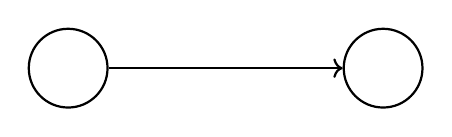
\begin{tikzpicture}[term/.style={circle,draw,minimum size=10mm,inner sep=5pt},auto]
    \node [thick] (s) at (0,0) [term] {$\stok$};
    \node [thick] (f) at (4,0) [term] {$\ftok$};
    \draw [->,thick] (s) to (f);
  \end{tikzpicture}
\end{center}

Additionally, we need rules relating these tokens to Hoare triples:
\begin{mathpar}
  \inferH{Ht-token-alloc}
  {T \in \{\stok, \ftok\} \and
    S \proves \hoare{\Exists \gamma.\ownGhost{\gamma}{T} \ast P}{e}{v.Q}}
  {S \proves \hoare{P}{e}{v.Q}}
  \and
  \inferH{Ht-token-update-pre}
  {S \proves \hoare{\ownGhost{\gamma}{\ftok} \ast P}{e}{v.Q}}
  {S \proves \hoare{\ownGhost{\gamma}{\stok} \ast P}{e}{v.Q}}
  \and
  \inferH{Ht-token-update-post}
  {S \proves \hoare{P}{e}{v.\ownGhost{\gamma}{\stok} \ast Q}}
  {S \proves \hoare{P}{e}{v.\ownGhost{\gamma}{\ftok} \ast Q}}
\end{mathpar}
%
Using these rules, we now
prove \eqref{eq:proving-parallel-increments-increase-at-least-by-one}.
The invariant we pick is the following predicate,
parametrised by $\gamma \in \textlog{GhostName}$.
\begin{align*}
  I(\gamma) = \Exists m. \ell \pointsto m \ast \left(\left(\ownGhost{\gamma}{\stok} \land m \geq n\right) \lor
                                                     \left(\ownGhost{\gamma}{\ftok} \land m \geq (n+1)\right)\right)
\end{align*}
%
The idea is as explained above.  The invariant can be in two
``states''.  It will be allocated in the first state, with the
``start'' token $\stok$, since we know that the current value stored
at $\ell$ is at least $n$.  Then, when a thread increases the value
stored at $\ell$, we
will update the invariant, so that it is in the ``finished'' state.
This pattern of using special ghost state tokens and disjunction to
encode information about the execution of the program in the invariant
is typical, and we shall see more of it later.

\begin{example}
  \label{example:parallel-increment-at-least-1}
So, let us start proving.
We start off by using the rule \ruleref{Ht-token-alloc} plus
\ruleref{Ht-exist}, so we have to prove
\begin{align*}
  \hoare{\ownGhost{\gamma}{\stok} \ast \ell \pointsto n}{(e \parcomp e) ; \deref \ell}{v.v \geq n + 1}.
\end{align*}
We then again use the sequencing rule \ruleref{Ht-seq}, but this time
the intermediate proposition is not $\TRUE$, but
$\ownGhost{\gamma}{\ftok}$, \ie{} we prove the following two triples
\begin{align}
  &\hoare{\ownGhost{\gamma}{\stok} \ast \ell \pointsto n}{e \parcomp e}{v.\ownGhost{\gamma}{\ftok}}\\
  &\hoare{\ownGhost{\gamma}{\ftok}}{\deref \ell}{v.v \geq n+1}.
    \label{eq:parallel-increments-second-triple}
\end{align}
We begin by showing the first triple.  Start by using the invariant
allocation rule \ruleref{Ht-inv-alloc}.  This is allowed by an
application of the rule of consequence \ruleref{Ht-csq} since
$\ownGhost{\gamma}{\stok} \ast \ell \pointsto n$ implies $I(\gamma)$.
Hence we have to prove
\begin{align*}
  \knowInv{\iota}{I(\gamma)} \proves \hoare{\TRUE}{e \parcomp e}{v.\ownGhost{\gamma}{\ftok}}.
\end{align*}
Since $\ownGhost{\gamma}{\ftok} \ast \ownGhost{\gamma}{\ftok}$ implies $\ownGhost{\gamma}{\ftok}$ it suffices (by the rule of consequence) to use the parallel composition rule \ruleref{Ht-par} and prove 
\begin{align*}
  \knowInv{\iota}{I(\gamma)} \proves \hoare{\TRUE}{e}{v.\ownGhost{\gamma}{\ftok}}.
\end{align*}
%
Again, using the bind rule, we first need to prove
\begin{align*}
  \knowInv{\iota}{I(\gamma)} \proves \hoare{\TRUE}{\deref \ell}{v.v \geq n}.
\end{align*}
Exercise!

For the other premise of the bind rule, we now have to show
\begin{align*}
  \knowInv{\iota}{I(\gamma)} \proves \hoare{m \geq n}{\ell \gets (m + 1)}{\_.\ownGhost{\gamma}{\ftok}}.
\end{align*}
To open the invariant we need an atomic expression.
We use the rule \ruleref{Ht-bind-det} to evaluate $m + 1$ to a value using the rule \ruleref{Ht-op}.
We then open the invariant and after using the rule \ruleref{Ht-disj} and other structural rules we need to prove the following two triples
\begin{align*}
  &\knowInv{\iota}{I(\gamma)} \proves \hoare{\later (\ell \pointsto m \ast \ownGhost{\gamma}{\stok} \land m \geq n)}
    {\ell \gets (m + 1)}{\_.\later I(\gamma) \ast \ownGhost{\gamma}{\ftok}}\\
  &\knowInv{\iota}{I(\gamma)} \proves \hoare{\later (\ell \pointsto m \ast \ownGhost{\gamma}{\ftok} \land m \geq (n+1))}
    {\ell \gets (m + 1)}{\_.\later I(\gamma) \ast \ownGhost{\gamma}{\ftok}}
\end{align*}
We only show the first one, and leave the second one as an exercise.
We note however that duplicability of $\ownGhost{\gamma}{\ftok}$ is essential.

Using the rules \ruleref{Ht-frame-atomic} and \ruleref{Ht-store} we derive the following entailment.
\begin{align*}
  &\knowInv{\iota}{I(\gamma)} \proves
    \hoare{\later (\ell \pointsto m \ast \ownGhost{\gamma}{\stok} \land m \geq n)}
    {\ell \gets (m + 1)}{v.v = () \land \ell \pointsto (m + 1) \ast \ownGhost{\gamma}{\stok} \land m \geq n}
\end{align*}
Following up with \ruleref{Ht-token-update-post} we get
\begin{align*}
  &\knowInv{\iota}{I(\gamma)} \proves
    \hoare{\later (\ell \pointsto m \ast \ownGhost{\gamma}{\stok} \land m \geq n)}
    {\ell \gets (m + 1)}{v.v = () \land \ell \pointsto (m + 1) \ast \ownGhost{\gamma}{\ftok} \land m \geq n}
\end{align*}
from which it is easy to derive the wanted triple using \textsc{\ftok-duplicable} to create another copy of $\ownGhost{\gamma}{\ftok}$.
One of the copies is used to reestablish the invariant $I(\gamma)$, and the other remains in the postcondition.

To conclude the proof of this example we now need to show \eqref{eq:parallel-increments-second-triple}
\begin{align*}
  \knowInv{\iota}{I(\gamma)} \proves \hoare{\ownGhost{\gamma}{\ftok}}{\deref \ell}{v.v \geq n + 1}
\end{align*}
%
Using the invariant opening rule \ruleref{Ht-inv-open} together with
structural rules we need to prove
\begin{align*}
  &\knowInv{\iota}{I(\gamma)} \proves \hoare{\ownGhost{\gamma}{\ftok} \ast \later (\ell \pointsto m \ast \ownGhost{\gamma}{\stok} \land m \geq n)}
    {\deref \ell}{v.v \geq (n + 1) \land \later I(\gamma)}\\
  &\knowInv{\iota}{I(\gamma)} \proves
    \hoare{\ownGhost{\gamma}{\ftok} \ast \later (\ell \pointsto m \ast \ownGhost{\gamma}{\ftok} \land m \geq (n + 1))}
    {\deref \ell}{v.v \geq (n + 1) \land \later I(\gamma)}
\end{align*}
By \textsc{\stok-\ftok-incompatible}, the precondition of the first triple is equivalent to $\later\FALSE$, that is, this case is \emph{impossible}, and the triple holds by \ruleref{Ht-later-false}.
We leave the second triple as an exercise.

To recap, the high-level idea of the proof is that the invariant can
be in two ``states''.  It starts off in the state where we know that
the value at $\ell$ is at least $n$ and then, when incrementing, we
transition to a new state, but we also get out a new token, \ie{} we
get $\ownGhost{\gamma}{\ftok}$ in the postcondition.  This token
is then used to decide in which case we are when opening the invariant
again.
\end{example}

\subsection{Ghost state}
\label{sec:ghost-state}

The ghost state used in the previous section was rather \emph{ad hoc}.
If we had to extend the logic with new primitive propositions for each new example, we would need to establish consistency for each such extension.
That is not tenable.
Thus in this section we develop a very general notion of resources.
It is not the most general notion of resources supported by Iris, but the final generalisation is quite technical and postponed until later sections.
Consistency of Iris with respect to this notion of resources will be proved in later sections.
The notion of resources described in this section suffices for the vast majority of program verifications.
However it is insufficient for certain more advanced uses of the logic, such as when Iris is used to reason about refinement, or when building the Iris program logic on top of the base logic.

\newcommand{\valid}{\mathcal{V}}

To define the notion of resources we need to recall some concepts and facts.
\begin{definition}
  A \emph{commutative semigroup} is a set $\Ml$ together with a function
  $(\cdot) : \Ml \times \Ml \to \Ml$, called the \emph{operation} such that
  the operation is associative and commutative.

  A commutative semigroup is called a \emph{commutative monoid} if there exists an 
  element $\eps$ (called the unit) which is the neutral element for the operation $(\cdot)$: for all
    $m \in \Ml$, the property $m \cdot \eps = \eps \cdot m = m$ holds.

  The set $\Ml$ is called the \emph{carrier} of the semigroup (resp.~monoid).
\end{definition}

Every semigroup can be made a preorder by defining the \emph{extension order} $a \mincl b$ as
\begin{align*}
  a \mincl b \iff \exists c, b = a \cdot c.
\end{align*}
In words, $a \mincl b$ if $a$ \emph{is a part of} $b$.
\begin{exercise}
  Show that the relation $\mincl$ is transitive for any semigroup $\Ml$.
  Show that it is reflexive if and only if for every element $a$ there exists an element $b \in \Ml$ such that $a \cdot b = a$.
  Conclude that if $\Ml$ is a commutative monoid then $\mincl$ is reflexive.
\end{exercise}


Certain kinds of commutative semigroups and monoids serve as good abstract models of resources.
Resources can be composed using the operation.
Commutativity and associativity express that the order in which resources are composed does not matter.
The unit of the monoid represents the empty resource, which exists in many instances.

Finally, we also need the ability to express that certain resources cannot be combined together.
This can be achieved in many ways.
The way we choose to do it is to have a subset $\Vl$ of so-called \emph{valid elements}.
Thus, for now, our notion of resources are the resource algebras defined as follows.%
\footnote{In general, resources in Iris can be elements of so-called ``cameras'' which are generalizations of \emph{resource algebras}.
  They add additional \emph{approximation information} to resources which is needed for the most advanced applications, however the vast majority of program verifications needs only the ``discrete cameras'', which is what we call resource algebras in these lecture notes.}
\begin{definition}[Resource algebra]
  \label{def:resource-algebra}
  A \emph{resource algebra} is a commutative semigroup $\Ml$ together with a subset $\Vl \subseteq \Ml$ of elements called \emph{valid}, and a \emph{partial} function $\mcore{\cdot} : \Ml \to \Ml$, called the \emph{core}.

  The set of valid elements is required to have the closure property
  \begin{align*}
    a \cdot b \in \Vl \implies a \in \Vl,
  \end{align*}
  that is, if $x$ is valid then every sub-part of $x$ is also valid.
  
  The core is required to have the following properties.
  \begin{align*}
    \mcore{a} \text{ defined} &\implies \mcore{a}\cdot a = a\\
    \mcore{a} \text{ defined} &\implies \mcore{\mcore{a}} = \mcore{a}\\
    a \mincl b \land \mcore{a} \text{ defined} &\implies \mcore{b} \text{ defined } \land \mcore{a} \mincl \mcore{b}.
  \end{align*}

  A resource algebra is \emph{unital} if $\Ml$ is a commutative monoid with unit $\eps$ and the following properties hold.
  \begin{mathpar}
    \eps \in \Vl \and \mcore{\eps} = \eps.
  \end{mathpar}
  In particular $\mcore{\eps}$ is defined.
\end{definition}
The core of the resource algebra is meant to be a function, which for each element captures the ``duplicable part'' of an element.
Sometimes such a duplicable part does not exist, hence we allow the core to be a partial function; we will see some such examples below.
\begin{exercise}
  Show that for any resource algebra $\Ml$, and any element $a \in \Ml$, the core of $a$, if defined, is duplicable, \ie{} for any $a$, show
  \begin{align*}
    \mcore{a} \text{ defined} \implies \mcore{a} \cdot \mcore{a} = \mcore{a}.
  \end{align*}
\end{exercise}


\begin{exercise}
  \label{exercise:unital-ra-core-total}
  Show that in a unital resource algebra the core is always defined.
  Hint: $\eps \mincl a$ for any element $a$.
\end{exercise}


\begin{example}
  \label{example:unital-resource-algebra-of-heaps}
  A canonical example of a unital resource algebra is the one of heaps.
  More precisely, the carrier of the resource algebra is the set of heaps plus an additional element, call it $\bot$, which is used to define composition of incompatible heaps.
  Composition of heaps is disjoint union, and if the heaps are not disjoint, then their composition is defined to be $\bot$.
  Composing $\bot$ with any other element yields $\bot$.
  The core is the constant function, mapping every element to the empty heap, which is the unit of the resource algebra.
  Every heap is valid, the only non-valid element being $\bot$.
\end{example}

\begin{example}
  \label{example:agreement-resource-algebra}
  We now present an example, which we will use later, and where the core is non-trivial.
  (It is closely related to the \emph{agreement construction}, which we will also use later on.)
  Given a set $X$, the carrier of the resource algebra is the set $X \cup \{\bot\}$, for some element $\bot$ not in $X$.
  The operation $(\cdot)$ is defined by the following rules.
  The non-trivial compositions are only
  \begin{mathpar}
    m \cdot m = m
  \end{mathpar}
  and otherwise (when $m$ and $n$ are distinct) $m \cdot n = \bot$.
  The core can be defined as the identity function, and every element apart from $\bot$ is valid.
  The definition of the core as the identity function is possible since every element of the resource algebra is duplicable.
\end{example}

\begin{example}[Finite subsets of natural numbers]
  \label{example:finite-subset-resource-algebra}
  The carrier of this resource algebra is the set of finite subsets of natural numbers and an additional element $\bot$. The operation is disjoint union, i.e.:
  \begin{align*}
    x \cdot y = 
    \begin{cases}
      x \cup y & \text{ if } x \cap y = \emptyset\\
      \bot & \text{ otherwise }
    \end{cases}
  \end{align*}

The unit of this operation is $\emptyset$. Valid elements are all finite subsets of natural numbers and the core operation maps every valid element to $\emptyset$.
\end{example}

\begin{example}
  \label{example:two-state-transition-system-ra}
  If we take the resource algebra $M$ to have the carrier $\{\stok, \ftok,\bot\}$ with multiplication defined as $\ftok \cdot \ftok = \ftok$ and otherwise $x \cdot y = \bot$ then, with the rules presented above, we can recover the rules \textsc{ftok-duplicable}, \textsc{\stok-\stok-incompatible} and \textsc{\stok-\ftok-incompatible}, which were postulated in the previous section.
  The core of the resource algebra $M$ is always undefined.
\end{example}

\begin{example}[Resource algebra of fractions]
  \label{example:resource-algebra-of-fractions}
  An often used resource algebra is the one of fractions $\QQ_{01}$.
  Its carrier is the set of (strictly) positive rational numbers $q$ with addition as the operation.
  However the valid elements are only those $q$ less than or equal to $1$, \ie{} ${\Vl = \left\{ q \isetsep 0 < q \leq 1 \right\}}$.
  The core is always undefined.
\end{example}

\begin{example}[Exclusive resource algebra]
  \label{ex:exclusive-resource-algebra}
  Given a set $X$ the exclusive resource algebra $\exm(X)$ has as carrier the set $X$ with an additional element $\bot$.
  The operation is defined such that $x \cdot y = \bot$ for all $x$ and $y$.
  The core is the always undefined function, and the valid elements are elements of $X$, \ie{} every element of the resource algebra except the $\bot$.

  Perhaps it does not seem that this resource algebra is very interesting.
  In fact it does appear in verification of certain programs, but it can also be used as a building block of other resource algebras, as shown in the following exercise.
\end{example}

The following examples are generic constructions.
They construct resource algebras combined from a variety of smaller ones.
This makes it easier to build more complex notions of resources needed in verification, since a lot of the infrastructure can be reused.
However it does take some practice to get used to thinking in terms of decomposition of the desired resource algebra in terms of the smaller ones.
We hope the reader will get some intuition for this by working through the example verifications in the rest of these notes.

\begin{example}[Products of resource algebras]
  If $\Ml_1$ and $\Ml_2$ are resource algebras with cores $\mcore{\cdot}_1$ and $\mcore{\cdot}_2$ and sets of valid elements $\Vl_1$ and $\Vl_2$ then we can form the product resource algebra $\Ml_\times$.
  Its carrier is the product $\Ml_1 \times \Ml_2$, and its operation is defined component-wise as
  \begin{align*}
    (a, b) \cdot (a', b') = (a \cdot a', b \cdot b')
  \end{align*}
  and the set of valid elements
  \begin{align*}
    \Vl_\times = \left\{(a, b) \isetsep a \in \Vl_1, b \in \Vl_2\right\}.
  \end{align*}
  The core is similarly defined component-wise as
  \begin{align*}
    \mcore{(a, b)}_\times =
    \begin{cases}
      \left(\mcore{a}_1, \mcore{b}_2\right) & \text{ if } \mcore{a}_1 \text{ and } \mcore{b}_2 \text{ defined}\\
      \text{undefined} & \text{ otherwise }
    \end{cases}
  \end{align*}
  It is easy to see (exercise!) that if both resource algebras are unital then so is the product resource algebra.

  This product example can be extended to a product of arbitrary many resource algebras.
\end{example}

\begin{example}[Finite map resource algebra]
  Let $(\Ml, \Vl, \mcore{\cdot})$ be a resource algebra.
  We can form a new resource algebra $\NN \finparmap \Ml$ whose carrier is the set of partial functions from $\NN$ to $\Ml$ with finite domain, and the operation is defined as
  \begin{align*}
    (f \cdot g)(n) =
    \begin{cases}
      f(n) \cdot g(n) & \text{ if } f(n) \text{ and } g(n) \text{ defined}\\
      f(n) & \text{ if } f(n) \text{ defined and} g(n) \text{ undefined}\\
      g(n) & \text{ if } g(n) \text{ defined and} f(n) \text{ undefined}\\
      \text{ undefined} & \text{ otherwise}
    \end{cases}
  \end{align*}
  The set of valid finite maps is
  \begin{align*}
    \Vl_{\NN \finparmap \Ml} = \left\{f \isetsep \forall n, f(n) \text{ defined} \implies f(n) \in \Vl\right\}
  \end{align*}
  and the core is defined as
  \begin{align*}
    (\mcore{f}_{\NN \finparmap \Ml})(n) =
    \begin{cases}
      \mcore{f(n)} & \text{ if } f(n) \text{ and } \mcore{f(n)} \text{ defined }\\
      \text{ undefined} & \text{ otherwise }
    \end{cases}
  \end{align*}
  Note that $\NN \finparmap \Ml$ is always a \emph{unital} resource algebra, its unit being the always undefined finite partial function.
\end{example}

\begin{exercise}
  Show that when restricted to valid elements, the resource algebra $\NN \finparmap \exm\left(\Val\right)$ is the same as the unital resource algebra of heaps described in Example~\ref{example:unital-resource-algebra-of-heaps}.
  More precisely, show that the valid elements of $\NN \finparmap \exm\left(\Val\right)$ are precisely the heaps, and composition of these is exactly the same as the composition of heaps, if it is a valid element.
\end{exercise}


\begin{example}[Option resource algebra]
  \label{example:option-resource-algebra}
  Given any resource algebra (not necessarily unital) $\Ml$, we define the unital resource algebra $\Ml_?$.
  Its carrier is the set $\Ml$ together with a new element $?$.
  The operation on elements of $\Ml$ is inherited, and we additionally set $? \cdot x = x \cdot ? = x$, \ie{} $?$ is the unit.
  The set of valid elements is that of $\Ml$ and $?$.
  Finally, the core operation is defined as
  \begin{align*}
    \mcore{?}_{\Ml_?} &={} ?\\
    \mcore{x}_{\Ml_?} &=
                \begin{cases}
                  \mcore{x} & \text{ if } \mcore{x} \text{ defined}\\
                  ? & \text{ otherwise}
                \end{cases}
  \end{align*}
\end{example}

\paragraph*{Extending Iris with resource algebras}
With these concepts, we can extend Iris with a general notion of resources, a single unital resource algebra.
Strictly speaking the logic is extended with a family of chosen resource algebras $\Ml_i$, which we leave open, so that new ones can be added when they are needed in the verification of concrete examples.
We add the resource algebras, and its elements, the core function, and the property of the element being valid, as new types and new terms of the logic, together with all the equations for the operations.
In addition to this we also add the notion of ghost names.
These are used to be able to refer to multiple different instances of the same resource algebra element, analogous to how different locations in a heap are used to contain different values.

Thus we extend the logic with the following constructs
\begin{mathpar}
  \coretypingrule
  \and
  \validtypingrule
  \and
  \owntypingrule
\end{mathpar}
The first two are self-explanatory, they internalise the notions of the resource algebra into the logic, \ie{} they allow us to reason about elements of the resource algebras in the logic.
The last rule introduces a new construct, the \emph{ghost ownership assertion} $\ownGhost{\gamma}{a : \Ml_i}$, which we will write as $\ownGhost{\gamma}{a}$ when the resource algebra $\Ml_i$ is clear from the context.
This assertion states that we own an instance of a ghost resource $a$ named $\gamma$.

The rules of the ghost ownership assertion are as follows.
\begin{mathpar}
  \ownoprule
  \and
  \ownvalidrule
\end{mathpar}
And the final rule, which shows why the core is useful, is related to the persistently modality with the following law of the logic.
\begin{mathpar}
  \perscorerule
\end{mathpar}

\paragraph*{Ghost updates}
We now consider how to update the ghost resources.
This ability will be used to evolve the ghost state along with the execution of the program.
When the ghost state changes, it is important that it remains valid -- Iris always maintains the invariant that the ghost state obtained by composing the contributions of all threads is well-defined and valid, \ie{} that all the contributions of all threads are compatible.
We call state changes that maintain this invariant \emph{frame-preserving updates}.

\begin{definition}[Frame preserving update]
  \label{def:frame-preserving-update}
  For any resource algebra $\Ml$ with the set of valid elements $\Vl$ we define a relation, the \emph{frame preserving update} $a \mupd B$, where $a \in \Ml$ and $B \subseteq \Vl$ is a \emph{non-empty} subset of valid elements.
  It states that any element compatible with $a$ is compatible with \emph{some} element in $B$.
  Precisely,
  \begin{mathpar}
    \fpurule
  \end{mathpar}
  If $B$ is the singleton set $\{b\}$, we write $a \mupd b$ for $a \mupd \{b\}$.
\end{definition}
%
To support modification of ghost state in the logic we introduce a new
\emph{update modality} $\pvs P$, with associated frame preserving
updates.  The typing rules and basic axioms of the update modality are
show in Figure~\ref{fig:pvs}.  The intuition is that $\pvs P$ holds
for a resource $r$, if from $r$ we can do a frame-preserving update to
some $r'$ that satisfies $P$. Thus the update modality $\pvs P$
provides a way, inside the logic, to talk about the resources we
\emph{could} own after performing an update to what we \emph{do} own.
With this intuitive reading of $\pvs P$, the laws in
Figure~\ref{fig:pvs} should make sense. For instance, the
\ruleref{upd-frame} axiom holds because if $r$ satisfies
$P \ast \pvs Q$, then $r$ can be split into $r_1$ and $r_2$ with
$r_1$ in $P$ and $r_2$ in $\pvs Q$, and the latter means that $r_2$
can be updated in a frame-preserving way to some $r'_2$ in $Q$, \ie{}
$r_2\mupd r'_2$.  But then also
$r=(r_1 \cdot r_2) \mupd (r_1 \cdot r'_2)$ and hence
$r\in\pvs (P \ast Q)$.

\begin{figure}[htbp]
  \centering
\begin{mathpar}
  \updtypingrule
  \and
  \updmonorule
  \and
  \updintrorule
  \and
  \updidemprule
  \and
  \updframerule
\end{mathpar}
  \caption{Laws for the update modality}
  \label{fig:pvs}
\end{figure}

\begin{exercise}
\label{exercise:basic-properties-of-primitive-view-shift}
  Show the following derived rules.
  \begin{enumerate}
  \item
    \begin{mathpar}
      \infer{P_1 \proves Q_1 \and P_2 \proves \pvs Q_2}
      {P_1 \ast P_2 \proves \pvs (Q_1 \ast Q_2)}
    \end{mathpar}
  \item 
    \begin{mathpar}
      \updseprule
    \end{mathpar}
  \item
    \begin{mathpar}
      \updbindrule
    \end{mathpar}
  \end{enumerate}
\end{exercise}


\begin{remark}
  Note that the rule \ruleref{upd-bind} is a kind of bind or let rule.
  Indeed, it may be instructive to compare the rule \ruleref{upd-bind}
  with the typing rule for a let construct in an ML-like language
\begin{mathpar}
  \infer
  {\Gamma \proves e_1 : \tau \and \Gamma, x : \tau \proves e_2 : \sigma}
  {\Gamma \proves \Let x = e_1 in e_2 : \sigma}
\end{mathpar}
The difference is that because of the use of separating conjunction we
need to separate the resources needed to prove $\pvs Q$ from those
needed to prove the $\pvs R$.  Thus we cannot use $P_2$ anymore when
proving $\pvs R$.
Instead \ruleref{upd-bind} very closely corresponds to the let rule in a language with an affine or linear type system.

The following exercise shows that if a more standard let-like rule is
added to the logic then the update modality would become significantly weaker.
\end{remark}

\begin{exercise}
  Show that if the rule
  \begin{mathpar}
    \infer{P \proves \pvs Q \and P \ast Q \proves \pvs R} {P \proves \pvs R}
  \end{mathpar}
  is added to the logic then the following is derivable for any $R$.
  \begin{mathpar}
    \infer
    {P \ast P \proves \FALSE}
    {P \proves \pvs R}
  \end{mathpar}
  In particular $P \proves \pvs \FALSE$ for $P$ such that $P \ast P \proves \FALSE$.
\end{exercise}


The update modality allows us to allocate 
and update ghost resources, as explained by the following rules.
\begin{mathpar}
  \ghostallocrule
  \and
  \ghostupdaterule
\end{mathpar}

Finally, we connect the update modality with Hoare triples.  The idea
is that ghost state is abstract state used to keep track of auxiliary
facts during proofs.  So we should be able to update the
ghost state in pre- and postconditions of Hoare triples,
since whether or not the program is safe to run, and its return value, only depends on the physical state.

A uniform way to do this is to generalise the consequence rule \ruleref{Ht-csq}.
We first define the \emph{view shift} $P \vs Q$ as
\begin{align*}
  P \vs Q = \persistently(P \implies \pvs Q)
\end{align*}
The generalized rule of consequence is then 
\begin{mathpar}
  \htcsqvsrule
\end{mathpar}
\begin{exercise}
  Derive the previous rule of consequence from the one just introduced.
\end{exercise}


\begin{exercise}
  \label{exercise:basic-properties-of-view-shift}
  Derive the following.
  
  \begin{itemize}
  \item
    \begin{align*}
      \infer
      {a \in \Vl}
      {P \proves \pvs \left(\left(\Exists \gamma.\ownGhost{\gamma}{a}\right) \ast P\right)}
    \end{align*}
  \item 
    \begin{displaymath}
      \infer
      {a \in \Vl}
      {\proves P \vs \left(\Exists \gamma.\ownGhost{\gamma}{a}\right) \ast P} \qedhere
    \end{displaymath}
  \end{itemize}
\end{exercise}


In particular, we have $\TRUE \vs \Exists \gamma.\ownGhost{\gamma}{a}$, for all valid $a$, and if $a \mupd b$ then $\ownGhost{\gamma}{a} \vs \ownGhost{\gamma}{b}$.
\begin{exercise}
  Derive the rest of the rules for start and finish tokens used in the previous section for the resource algebra from Example~\ref{example:two-state-transition-system-ra}.
  That is, show the rules \ruleref{Ht-token-update-post}, \ruleref{Ht-token-update-pre}, and \ruleref{Ht-token-alloc}.
\end{exercise}


\begin{exercise}[Allocating invariants in the post-condition]
  \label{exercise:allocating-invariants-postcondition}
  It will often be the case that we need to allocate an invariant in the post-condition, using the following derivable rule.
  \begin{mathpar}
    \htinvallocpostrule
  \end{mathpar}
  Derive the rule using \ruleref{Ht-inv-alloc}, the fact that invariants are persistent and the generalised rule of consequence introduced above.
\end{exercise}


\begin{example}
  \label{ex:precise-spec-of-parallel-increment}
  In this example we show how to use slightly more complex reasoning using resource algebras to show the specification~\eqref{eq:precise-spec-of-parallel-increment} (page~\pageref{eq:precise-spec-of-parallel-increment}) from the parallel increment example.
  We are going to use two resource algebras: the one of fractions defined in Example~\ref{example:resource-algebra-of-fractions} together with the resource algebra encoding the transition system with states $\stok$ and $\ftok$ defined in Example~\ref{example:two-state-transition-system-ra} and demonstrated in Example~\ref{example:parallel-increment-at-least-1}.
  
  The proof proceeds similarly to the proof in Example~\ref{example:parallel-increment-at-least-1}, but with a different invariant.
  The invariant we are going to use is
  \begin{align*}
    I(\gamma_1, \gamma_2, n) =\ &\ell \pointsto n \ast \ownGhost{\gamma_1}{\stok} \lor\\
                                &\ell \pointsto (n+1) \ast \ownGhost{\gamma_1}{\ftok} \ast \ownGhost{\gamma_2}{\frac{1}{2}}\lor\\
                                &\ell \pointsto (n+2) \ast \ownGhost{\gamma_1}{\ftok} \ast \ownGhost{\gamma_2}{1}
  \end{align*}
  That is, we are in essence encoding a three state transition system.
  The tokens $\ftok$ and $\stok$ are used to distinguish the initial state from the rest of the states, and the fractions $\frac{1}{2}$ and $1$ can be thought of as the price needed to get from the initial state to the current state.
  We can depict this in the following way
  \begin{center}
    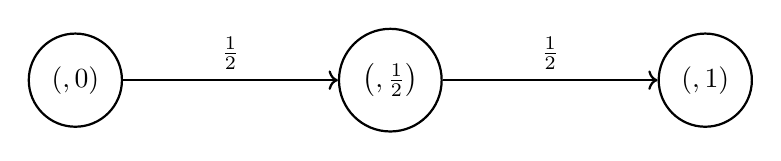
\begin{tikzpicture}[term/.style={circle,draw,minimum size=10mm,inner sep=5pt},auto]
      \node [thick] (s) at (0,0) [term] {$(\stok, 0)$};
      \node [thick] (f1) at (4,0) [term] {$\left(\ftok, \frac{1}{2}\right)$};
      \node [thick] (f2) at (8,0) [term] {$(\ftok, 1)$};
      \draw [->,thick] (s) to node {$\frac{1}{2}$} (f1);
      \draw [->,thick] (f1) to node {$\frac{1}{2}$} (f2);
    \end{tikzpicture}
  \end{center}
  The resources on the transitions can also be viewed as coming from the environment.
  To make a transition from one state to another the environment will have to give up ownership of $\ownGhost{\gamma_2}{\frac{1}{2}}$ and transfer it to the invariant.

  With this invariant let us proceed to the proof of the specification
  \begin{align*}
    \hoare{\ell \pointsto n}{(e \parcomp e) ; \deref \ell}{v.v = n + 1 \lor v = n + 2}.
  \end{align*}
  We start off by allocating two pieces of ghost state.
  We allocate $\ownGhost{\gamma_1}{\stok}$ and $\ownGhost{\gamma_2}{1}$ for some $\gamma_1$ and $\gamma_2$ using the rule \ruleref{Ghost-alloc} and the generalized rule of consequence.
  Hence we have to show
  \begin{align*}
      \hoare{\ownGhost{\gamma_1}{\stok} \ast \ownGhost{\gamma_2}{1} \ast \ell \pointsto n}{(e \parcomp e) ; \deref \ell}{v.v = n + 1 \lor v = n + 2}.
  \end{align*}
  Using the invariant allocation rule we allocate the invariant by transferring
  \begin{align*}
    \ownGhost{\gamma_1}{\stok} \ast \ell \pointsto n
  \end{align*}
  into the invariant, which then means we have to show
  \begin{align*}
    \knowInv{\iota}{I(\gamma_1,\gamma_2,n)} \proves \hoare{\ownGhost{\gamma_2}{1}}{(e \parcomp e) ; \deref \ell}{v.v = n + 1 \lor v = n + 2}
  \end{align*}
  for some $\iota$.
  Using the rule \ruleref{Ht-seq} we now verify the two parts, showing the following two triples
  \begin{align*}
    \knowInv{\iota}{I(\gamma_1,\gamma_2,n)} &\proves \hoare{\ownGhost{\gamma_2}{1}}{(e \parcomp e)}{\_.\ownGhost{\gamma_1}{\ftok}}\\
    \knowInv{\iota}{I(\gamma_1,\gamma_2,n)} &\proves \hoare{\ownGhost{\gamma_1}{\ftok}}{\deref \ell}{v.v = n + 1 \lor v = n + 2}.\\
  \end{align*}
  The proof of the second triple is completely analogous to the one in Example~\ref{example:parallel-increment-at-least-1}, so we omit it here.
  To show the first triple we first use the rule \ruleref{Own-op} to get
  \begin{align*}
    \ownGhost{\gamma_2}{1} \iff \ownGhost{\gamma_2}{\frac{1}{2}} \ast \ownGhost{\gamma_2}{\frac{1}{2}}
  \end{align*}
  and 
  \begin{align*}
    \ownGhost{\gamma_1}{\ftok} \iff \ownGhost{\gamma_1}{\ftok} \ast \ownGhost{\gamma_1}{\ftok}
  \end{align*}
  and hence the first triple is equivalent to
  \begin{align*}
    \knowInv{\iota}{I(\gamma_1,\gamma_2,n)} &\proves \hoare{\ownGhost{\gamma_2}{\frac{1}{2}} \ast \ownGhost{\gamma_2}{\frac{1}{2}}}{(e \parcomp e)}{\_.\ownGhost{\gamma_1}{\ftok} \ast \ownGhost{\gamma_1}{\ftok}}
  \end{align*}
  which means we can use the parallel composition rule \ruleref{Ht-par}, and we have to show
  \begin{align*}
    \knowInv{\iota}{I(\gamma_1,\gamma_2,n)} &\proves \hoare{\ownGhost{\gamma_2}{\frac{1}{2}}}{e}{\_.\ownGhost{\gamma_1}{\ftok}}.
  \end{align*}
  Recall that $e$ is the program $\ell \gets \deref \ell + 1$.
  Using the \ruleref{Ht-bind} rule we show the following two entailments.
  \begin{align}
    \label{eq:parallel-increment-reading-spec}
    \knowInv{\iota}{I(\gamma_1,\gamma_2,n)} &\proves \hoare{\ownGhost{\gamma_2}{\frac{1}{2}}}{\deref \ell}{v.\left(v = n \lor v = (n+1) \ast \ownGhost{\gamma_1}{\ftok}\right) \ast \ownGhost{\gamma_2}{\frac{1}{2}}}\\
    \label{eq:parallel-increment-writing-spec}
    \knowInv{\iota}{I(\gamma_1,\gamma_2,n)} &\proves \All v .\hoare{\left(v = n \lor v = (n+1) \ast \ownGhost{\gamma_1}{\ftok}\right)\ast \ownGhost{\gamma_2}{\frac{1}{2}}}{\ell \gets v + 1}{\_.\ownGhost{\gamma_1}{\ftok}}
  \end{align}
  Note the $\ownGhost{\gamma_1}{\ftok}$ token we chose to add in the postcondition for the case of reading $n+1$. As in Example~\ref{example:parallel-increment-at-least-1}, this is essential to show the second triple: with $\ownGhost{\gamma_1}{\ftok}$ being duplicable, this allows us to \emph{remember} that the invariant is not in the initial state anymore.
  Then, when storing, we can exclude the impossible case where we store $n+2$ (and thus must have read $n+1$) while the invariant is still in the initial state $\ownGhost{\gamma_1}{\stok}$ (in which case we would not be able to reestablish the invariant, as we only have one $\ownGhost{\gamma_2}{\frac{1}{2}}$ fraction).
  As in this case we will have ownership of both the S and the F token (which are incompatible), we will be able to reach a contradiction.

  We first show \eqref{eq:parallel-increment-reading-spec} and start by opening the invariant $I(\gamma_1,\gamma_2,n)$.
  We thus get
  \begin{align*}
    \later\left(\ell \pointsto n \ast \ownGhost{\gamma_1}{\stok} \lor \ell \pointsto (n+1) \ast \ownGhost{\gamma_1}{\ftok} \ast \ownGhost{\gamma_2}{\frac{1}{2}}\lor                               \ell \pointsto (n+2) \ast \ownGhost{\gamma_1}{\ftok} \ast \ownGhost{\gamma_2}{1}\right) \ast \ownGhost{\gamma_2}{\frac{1}{2}}
  \end{align*}
  in the precondition which, using the distributivity laws of the logic, together with \ruleref{Own-op} simplifies to
  \begin{align*}
    &\later\left(\ell \pointsto n \ast \ownGhost{\gamma_1}{\stok}\right) \ast \ownGhost{\gamma_2}{\frac{1}{2}} \lor\\
    &\later \left(\ell \pointsto (n+1) \ast \ownGhost{\gamma_1}{\ftok} \ast \ownGhost{\gamma_2}{\frac{1}{2}}\right) \ast \ownGhost{\gamma_2}{\frac{1}{2}} \lor\\
    &\later\left(\ell \pointsto (n+2) \ast \ownGhost{\gamma_1}{\ftok} \ast \ownGhost{\gamma_2}{\frac{3}{2}}\right)
  \end{align*}
  The last disjunct is equivalent to $\later \FALSE$ by \ruleref{Own-valid} and the fact that the only valid fractions are those which are not greater than $1$.
  Using the disjunction rule \ruleref{Ht-disj} we have to show further three triples, all with postcondition 
  \begin{align*}
    \left(v = n \lor v = (n+1) \ast \ownGhost{\gamma_1}{\ftok}\right) \ast \ownGhost{\gamma_2}{\frac{1}{2}} \ast \later I(\gamma_1,\gamma_2,n)
  \end{align*}
  and with three preconditions corresponding to the three disjuncts above.
  The last is the easiest one and follows directly from \ruleref{Ht-later-false}.
  The first two we leave as exercises, since they are direct applications of rules we have seen many times.
  \begin{exercise}
    Show the following two triples.
    \begin{align*}
      &\hoare{\later\left(\ell \pointsto n \ast \ownGhost{\gamma_1}{\stok}\right) \ast \ownGhost{\gamma_2}{\frac{1}{2}}}{\deref \ell}{v.\left(v = n \lor v = (n+1) \ast \ownGhost{\gamma_1}{\ftok}\right) \ast \ownGhost{\gamma_2}{\frac{1}{2}} \ast \later I(\gamma_1,\gamma_2,n)}\\
      &\hoare{\later \left(\ell \pointsto (n+1) \ast \ownGhost{\gamma_1}{\ftok} \ast \ownGhost{\gamma_2}{\frac{1}{2}}\right) \ast \ownGhost{\gamma_2}{\frac{1}{2}}}{\deref \ell}{v.\left(v = n \lor v = (n+1) \ast \ownGhost{\gamma_1}{\ftok}\right) \ast \ownGhost{\gamma_2}{\frac{1}{2}} \ast \later I(\gamma_1,\gamma_2,n)}
    \end{align*}
  \end{exercise}
  
  
  Let us now turn to showing the specification \eqref{eq:parallel-increment-writing-spec}.
  Using the $\forall$ introduction rule, distributivity of $\ast$ over $\lor$, and \ruleref{Ht-disj} this means showing two specifications. 
  \begin{align}
    \label{eq:parallel-increment:read-n}
    \knowInv{\iota}{I(\gamma_1,\gamma_2,n)} &\proves \hoare{v = n \ast \ownGhost{\gamma_2}{\frac{1}{2}}}{\ell \gets v + 1}{\_.\ownGhost{\gamma_1}{\ftok}}\\
    \label{eq:parallel-increment:read-n-one}
    \knowInv{\iota}{I(\gamma_1,\gamma_2,n)} &\proves \hoare{v = (n+1) \ast \ownGhost{\gamma_1}{\ftok} \ast \ownGhost{\gamma_2}{\frac{1}{2}}}{\ell \gets v + 1}{\_.\ownGhost{\gamma_1}{\ftok}}
  \end{align}
  We show the first and leave the second as an exercise.
  Using \ruleref{Ht-persistently} and ordinary equational reasoning the first triple is equivalent to
  \begin{align*}
    \knowInv{\iota}{I(\gamma_1,\gamma_2,n)} &\proves \hoare{\ownGhost{\gamma_2}{\frac{1}{2}}}{\ell \gets n + 1}{\_.\ownGhost{\gamma_1}{\ftok}}
  \end{align*}
  To be completely precise we first need to use the bind rule to compute $n + 1$ to a value, but this is completely straighforward, so let us just assume we have done it.
  We then open the invariant and after simplifying we have
  \begin{align*}
    \later\left(\ell \pointsto n \ast \ownGhost{\gamma_1}{\stok} \ast \ownGhost{\gamma_2}{\frac{1}{2}}\right) \lor
    \later \left(\ell \pointsto (n+1) \ast \ownGhost{\gamma_1}{\ftok} \ast \ownGhost{\gamma_2}{1}\right) \lor
    \later\left(\ell \pointsto (n+2) \ast \ownGhost{\gamma_1}{\ftok} \ast \ownGhost{\gamma_2}{\frac{3}{2}}\right)
  \end{align*}
  in the precondition.
  As before, the last disjunct is equivalent to $\later\FALSE$ and the corresponding triple follows from \ruleref{Ht-later-false}.
  Using \ruleref{Ht-disj} we thus need to prove the following two specifications.
  \begin{align}
    \label{eq:parallel-increment:write:we-have-read-n}
    &\hoare{\later\left(\ell \pointsto n \ast \ownGhost{\gamma_1}{\stok} \ast \ownGhost{\gamma_2}{\frac{1}{2}}\right)}{\ell \gets n+1}{\_.\ownGhost{\gamma_1}{\ftok} \ast \later I(\gamma_1,\gamma_2,n)}\\
    \label{eq:parallel-increment:write:we-have-read-n-one}
    &\hoare{\later \left(\ell \pointsto (n+1) \ast \ownGhost{\gamma_1}{\ftok} \ast \ownGhost{\gamma_2}{1}\right)}{\ell \gets n+1}{\_.\ownGhost{\gamma_1}{\ftok} \ast \later I(\gamma_1,\gamma_2,n)}
  \end{align}
  We show the first and leave the second as an exercise.
  We proceed by forward reasoning and start by using \ruleref{Ht-load} and \ruleref{Ht-frame-atomic} to get
  \begin{align}
    \label{eq:1:needs-consequence}
    \hoare{\later\left(\ell \pointsto n \ast \ownGhost{\gamma_1}{\stok} \ast \ownGhost{\gamma_2}{\frac{1}{2}}\right)}{\ell \gets n+1}
    {\ell \pointsto n+1 \ast \ownGhost{\gamma_1}{\stok} \ast \ownGhost{\gamma_2}{\frac{1}{2}}}
  \end{align}
  We then use the fact that $\stok \mupd \ftok$ together with the rule \ruleref{Ghost-update} and \ruleref{upd-frame} to get
  \begin{align*}
    \left(\ell \pointsto n+1 \ast \ownGhost{\gamma_1}{\stok} \ast \ownGhost{\gamma_2}{\frac{1}{2}}\right) \vs \left(\ell \pointsto n+1 \ast \ownGhost{\gamma_1}{\ftok} \ast \ownGhost{\gamma_2}{\frac{1}{2}}\right)
  \end{align*}
  Moreover $\ftok = \ftok \cdot \ftok$ and thus \ruleref{Own-op} gives us $\ownGhost{\gamma_1}{\ftok} \vs \left(\ownGhost{\gamma_1}{\ftok} \ast \ownGhost{\gamma_1}{\ftok}\right)$ and thus together we have
  \begin{align*}
    \left(\ell \pointsto n+1 \ast \ownGhost{\gamma_1}{\stok} \ast \ownGhost{\gamma_2}{\frac{1}{2}}\right) \vs
    \left(\ell \pointsto n+1 \ast \ownGhost{\gamma_1}{\ftok} \ast \ownGhost{\gamma_1}{\ftok} \ast \ownGhost{\gamma_2}{\frac{1}{2}}\right).
  \end{align*}
  Clearly $\ell \pointsto n+1 \ast \ownGhost{\gamma_1}{\ftok} \ast \ownGhost{\gamma_2}{\frac{1}{2}} \vs \later I(\gamma_1,\gamma_2,n)$ and thus we have
  \begin{align*}
    \left(\ell \pointsto n+1 \ast \ownGhost{\gamma_1}{\stok} \ast \ownGhost{\gamma_2}{\frac{1}{2}}\right) \vs
    \left(\ownGhost{\gamma_1}{\ftok} \ast \later I(\gamma_1,\gamma_2,n)\right)
  \end{align*}
  and thus finally, by the (generalized) rule of consequence, we get \eqref{eq:parallel-increment:write:we-have-read-n} from \eqref{eq:1:needs-consequence}, as needed.
  
  \begin{exercise}
    Following similar reasoning illustrated above show specifications~\eqref{eq:parallel-increment:write:we-have-read-n-one} and~\eqref{eq:parallel-increment:read-n-one}.
  \end{exercise}
  

  The proof is somewhat complex, and perhaps the key new point, compared to previous examples (in particular Example~\ref{example:parallel-increment-at-least-1}), is lost to the reader.
  The key new way of reasoning in this example is the use of the fraction $\frac{1}{2}$ and how we transferred it from the ownership of a thread to the ownership of the invariant.
  Technically this can be seen from the fact that if when reading $\deref \ell$ the invariant is in state $\ell \pointsto n \ast \ownGhost{\gamma_1}{\stok}$, then after writing it is in state $\ell \pointsto (n+1) \ast \ownGhost{\gamma_1}{\ftok} \ast \color{red} \ownGhost{\gamma_2}{\frac{1}{2}}$.
  Analogously, if the invariant is in state
  $\ell \pointsto (n+1) \ast \ownGhost{\gamma_1}{\ftok} \ast \color{red} \ownGhost{\gamma_2}{\frac{1}{2}}$ when reading, then after writing it is in state $\ell \pointsto (n+2) \ast \ownGhost{\gamma_1}{\ftok} \ast \color{red} \ownGhost{\gamma_2}{1}$.
  Finally, we have used the fact that the threads own $\ownGhost{\gamma_2}{\frac{1}{2}}$ at the beginning, to discount the possibility that
  we have read the value $n+2$ before writing, \ie{} that the invariant was in state $\ell \pointsto (n+2) \ast \ownGhost{\gamma_1}{\ftok} \ast \color{red} \ownGhost{\gamma_2}{1}$.
\end{example}
\begin{exercise}
  For the same program $e$ as in the preceding example, define an invariant which would allow you to prove the following specification
  \begin{align*}
    \hoare{\ell \pointsto n}{\left((e \parcomp e) \parcomp e\right) ; \deref \ell}{v. v = n+1 \lor v = n+2 \lor v = n+3}.
  \end{align*}
\end{exercise}


\begin{example}
  \label{example:parallel-add}
  This example is a generalization of the parallel increment example~\ref{ex:precise-spec-of-parallel-increment}.
  Instead of for a fixed number of threads, we will prove a specification for any number of threads adding to a location.
  We also generalize it to the addition of any number instead of just $1$ for each thread.
  This is slightly more interesting, because the possible result values in the location are not just $n+1, n+2, \ldots, n+k$, but any combination of the numbers the threads are adding.
  As we will see, this does not allow us to use the same reasoning as in the previous example.
  Instead, we present another way of combining state-tracking resource algebras (multiple S-F instances), which at the same time represents an alternative way of proving the specification of Example~\ref{ex:precise-spec-of-parallel-increment}, without using the fractional resource algebra.

  Another new aspect of this example is that we show a specification for an inductively constructed program, namely a program consisting of any number of nested threads. As we will see in the proof, induction on the list of threads while having an invariant about those threads is not trivial.

  The program and specification for $k$ threads with numbers $a_1, \ldots, a_k$ to add is the following:
  \newcommand{\paralleladdprog}[1][k]{\left(e_1 \parcomp\;(e_2 \parcomp\;\cdots\;(e_{#1-1} \parcomp e_{#1})\cdots\right))}
  \begin{align}
    \label{eq:parallel-add-spec}
    \hoare{\ell \pointsto n}
    {\paralleladdprog \; ; \; \deref \ell}
    {v. \exists A \subseteq \{1,\dots,k\}\,,\; A \neq \emptyset \;\land\; v = n + \textstyle\sum_{i \in A}{a_i} }
  \end{align}
  where $e_i \;=\; \ell \gets \deref \ell + a_i$.

  The proof is structured as the one in Example~\ref{ex:precise-spec-of-parallel-increment}:
  We will have an invariant that governs the location $\ell$ and which can be in different states, logically representing which threads have contributed.
  One might think that we could proceed with fractions similarly to the example with two threads where instead of a fraction $\frac{1}{2}$, each thread would get a fraction corresponding to its contribution, \ie{} $\frac{a_j}{\sum_{i=1,\dots,k} a_i}$ for thread $j$, and the fractions collected in the invariant would represent the amount added to the location.
  However, this will not work out, as we will not be able to distinguish between the addition of an $a_i$ and two times the addition of $\frac{a_i}{2}$, for instance.
  This would allow to represent sums that in reality are not possible.

  Luckily, it turns out that the problem is much simpler and we do not even need fractions.
  What we actually want to track is whether a thread has contributed or not, to discount the possibility of a thread's number being contributed twice.
  This can be achieved with the two-state transition system with states S and F from Example~\ref{example:two-state-transition-system-ra} which we also have used in the previous proofs of parallel increment.
  We will simply use $k$ instances of this resource algebra, one for each thread.
  We use the ghost names $\overline\gamma = \gamma_1, \dots, \gamma_k$ to distinguish them.
  Additionally we will -- as before -- use the same transition system to encode the global state of execution, namely whether we are in the starting state S or a final state F.
  This instance is represented by the ghost name $\gamma$.
  With this idea, our invariant looks as follows:
  \begin{align*}
    I(\gamma,\overline\gamma, n) =\ \ell \pointsto n \ast \ownGhost{\gamma}{\stok} \;\lor\;
                                               \exists A \subseteq \{1,\dots,k\}\,,\; A \neq \emptyset \;\land\; \ell \pointsto n + \textstyle\sum_{i \in A}{a_i} \;\ast\; \Sep_{i \in A}\; \ownGhost{\gamma_i}{\ftok} \ast \ownGhost\gamma\ftok
  \end{align*}
  The invariant can be in two states. The first state, represented by the token $\ownGhost{\gamma}{\stok}$, is the same as in the example with just two threads: the value at the location is unchanged, as no thread has written to the location yet.
  The second state, represented by the token $\ownGhost{\gamma}{\ftok}$, represents all possible final states of the program, \ie{} where all threads have executed and thus the contribution of at least one thread has to have been added to $\ell$.
  For each thread whose number is included in the sum, we additionally have the thread-specific final state token $\ownGhost{\gamma_i}{\ftok}$.
  This allows us to exclude the impossible case where a thread's number is already part of the sum when it makes its contribution.

  Let us now show how we can prove specification \eqref{eq:parallel-add-spec} using this invariant.
  We start by allocating ghost state: the global $\ownGhost{\gamma}{\stok}$ token and the thread-specific $\ownGhost{\gamma_i}{\stok}$ tokens.
  Then the specification to show is
  \begin{align*}
    \hoareV{\ell \pointsto n \ast \ownGhost{\gamma}{\stok} \ast \textstyle{\Sep_{i \in \{1, \dots, k\}}}\; \ownGhost{\gamma_i}{\stok}}
    {\paralleladdprog \; ; \; \deref \ell}
    {v. \exists A \subseteq \{1,\dots,k\}\,,\; A \neq \emptyset \;\land\; v = n + \textstyle\sum_{i \in A}{a_i}\vphantom{\ownGhost{\gamma_i}{\stok}}}
  \end{align*}
  which allows us to allocate the invariant in the starting state, leaving us to show
  \begin{align*}
    \knowInv{\iota}{I(\gamma,\overline\gamma, n)}
    \proves \hoareV{\textstyle{\Sep_{i \in \{1, \dots, k\}}}\; \ownGhost{\gamma_i}{\stok}}
    {\paralleladdprog \; ; \; \deref \ell}
    {v. \exists A \subseteq \{1,\dots,k\}\,,\; A \neq \emptyset \;\land\; v = n + \textstyle\sum_{i \in A}{a_i}\vphantom{\ownGhost{\gamma_i}{\stok}}}
  \end{align*}
  As usual, we use the sequencing rule to prove two triples:
  \begin{align}
    \label{eq:parallel-add-main-spec}
    \knowInv{\iota}{I(\gamma,\overline\gamma, n)}
    &\proves \hoare{\textstyle{\Sep_{i \in \{1, \dots, k\}}}\; \ownGhost{\gamma_i}{\stok}}
    {\paralleladdprog}
    {\ignarg{} \ownGhost{\gamma}{\ftok}}\\
    \label{eq:parallel-add-reading-spec}
    \knowInv{\iota}{I(\gamma,\overline\gamma, n)}
    &\proves \hoare{\ownGhost{\gamma}{\ftok}}
    {\deref \ell}
    {v. \exists A \subseteq \{1,\dots,k\}\,,\; A \neq \emptyset \;\land\; v = n + \textstyle\sum_{i \in A}{a_i}\vphantom{\ownGhost{\gamma_i}{\stok}}}
  \end{align}
  Following the same pattern as in the examples \ref{example:parallel-increment-at-least-1} and \ref{ex:precise-spec-of-parallel-increment}, for the postcondition of the parallel part of the program we choose ownership of the $\ownGhost{\gamma}{\ftok}$ token.
  This is enough to get our eventual postcondition when reading the location in the second triple, as the token implies that the invariant must be in the final state.
  This part is completely analogous to the proofs before, so we leave showing \eqref{eq:parallel-add-reading-spec} as an exercise.

  To prove the main part, \eqref{eq:parallel-add-main-spec}, we need a specification for the individual threads, which we can then compose to prove the whole program:
  \begin{align}
    \label{eq:parallel-add-thread-spec}
    \knowInv{\iota}{I(\gamma,\overline\gamma, n)}
    &\proves \hoare{\ownGhost{\gamma_i}{\stok}}{e_i}{\ignarg{} \ownGhost{\gamma}{\ftok}}
  \end{align}
  That is, given the invariant and the thread-specific $\ownGhost{\gamma_i}{\stok}$ token, after executing $e_i$, we will have the global $\ownGhost{\gamma}{\ftok}$ token.
  This -- obtained from the invariant's final state -- represents the fact that after executing any one thread, the value stored at $\ell$ is a possible final value.
  Note that we do not need an $\ownGhost{\gamma_i}{\ftok}$ token here; these are only used in the invariant.

  With this specification, showing \eqref{eq:parallel-add-main-spec} seems trivial: we repeatedly use \ruleref{Ht-par} and will end up with $k$ $\ownGhost{\gamma}{\ftok}$ tokens, where one is enough for the required postcondition.
  Note however, that formally, we have to show this using induction on the number of threads $k$.
  This will not work directly, as $k$ also occurs in the invariant, namely in the list of ghost names $\overline\gamma = \gamma_1, \dots, \gamma_k$.
  This means that the induction hypothesis would work with a different invariant (for the threads $1, \dots, k-1$) and thus the two premises for the \ruleref{Ht-par} rule would have a different left side of the entailment and we would be stuck.
  The solution is to keep the invariant over the list of \emph{all} threads, while doing induction on a suffix of the list of threads not having considered yet (for which there must be an $\ownGhost{\gamma_i}{\stok}$ token and which at the beginning happen to be all threads).
  Note that the \ruleref{Ht-par} rule allows us to consider (prove) the threads in any order.
  Intuitively we can do it this way because the invariant's proposition for some of the threads also holds for all threads (if the result value is the sum of contributions from a subset of \emph{some} of the threads, then it is also the sum of contributions from a subset of \emph{all} threads).
  Technically it works because specification and proof for a single thread \eqref{eq:parallel-add-thread-spec} just talk about that single thread and are independent of the other threads.
  Formally, instead of showing \eqref{eq:parallel-add-main-spec}, we show the following triple for any $q \leq k$:
  \begin{align}
    \label{eq:parallel-add-main-spec-alt}
    \knowInv{\iota}{I(\gamma,\overline\gamma, n)}
    \proves \hoare{\textstyle{\Sep_{i \in \{1, \dots, q\}}}\; \ownGhost{\gamma_i}{\stok}}
    {\left(e_q \parcomp\;(e_{q-1} \parcomp\;\cdots\;(e_{2} \parcomp e_{1})\;\cdots\;)\right)}
      {\ignarg{} \ownGhost{\gamma}{\ftok}}
  \end{align}
  Induction is then straightforward.
  The base case $q = 1$ is exactly specification \eqref{eq:parallel-add-thread-spec} with $i = 1$.
  In the induction case, the induction hypothesis gives the specification \eqref{eq:parallel-add-main-spec-alt} for $q-1$, the one for $e_q$ is again \eqref{eq:parallel-add-thread-spec} (with $i = q$) and thus we can use the \ruleref{Ht-par} rule to obtain \eqref{eq:parallel-add-main-spec-alt}, just with post condition $\ownGhost{\gamma}{\ftok} \ast \ownGhost{\gamma}{\ftok}$, which we simplify to $\ownGhost{\gamma}{\ftok}$ using \ruleref{Ht-csq}.
  For $q = k$ we then get \eqref{eq:parallel-add-main-spec} from \eqref{eq:parallel-add-main-spec-alt}.
  
  We conclude the proof by showing the essential part, the specification \eqref{eq:parallel-add-thread-spec} for a single thread using the invariant.
  Recall that thread $e_j$ is the program $\ell \gets \deref \ell + a_j$.
  Using the \ruleref{Ht-bind} rule we show the following two entailments:
  \begin{align}
    \label{eq:parallel-add-thread-reading-spec}
    \knowInv{\iota}{I(\gamma,\overline\gamma, n)}
    &\proves &&\hoareV{\ownGhost{\gamma_j}{\stok}}
      {\deref \ell}
      {v.\; \ownGhost{\gamma_j}{\stok} \ast \left(v = n \lor \exists A \subseteq \{1,\dots,k\}\setminus\{j\}\,,\; A \neq \emptyset \;\land\; v = n + \textstyle\sum_{i \in A}{a_i} \ast \Sep_{i \in A}\; \ownGhost{\gamma_i}{\ftok} \ast \ownGhost{\gamma}{\ftok}\right)}&\\
    \label{eq:parallel-add-writing-spec}
    \knowInv{\iota}{I(\gamma,\overline\gamma, n)}
    &\proves \All v .\hspace*{-0.75em}&&\hoareV{\ownGhost{\gamma_j}{\stok} \ast \left(v = n \lor \exists A \subseteq \{1,\dots,k\}\setminus\{j\}\,,\; A \neq \emptyset \;\land\; v = n + \textstyle\sum_{i \in A}{a_i} \ast \Sep_{i \in A}\; \ownGhost{\gamma_i}{\ftok} \ast \ownGhost{\gamma}{\ftok}\right)}
      {\ell \gets v + a_j}
      {\ignarg{} \ownGhost{\gamma}{\ftok}}&
  \end{align}
  The idea is that if we read a value which includes the contributions from some threads, we want to remember that the invariant was in the corresponding state.
  This is done in \eqref{eq:parallel-add-thread-reading-spec} via the tokens $\ownGhost{\gamma}{\ftok}$ and $\ownGhost{\gamma_i}{\ftok}$ for all $i$ where the contribution $a_i$ is included in the read value.
  It is moreover important to include the fact that $a_j$ is not part of the read sum, which cannot be the case because the current thread has not written yet.
  We will see that this is needed in the proof of \eqref{eq:parallel-add-writing-spec}.
  To show \eqref{eq:parallel-add-thread-reading-spec} we open the invariant $I(\gamma,\overline\gamma,n)$ and get two disjuncts in the precondition.
  Using the \ruleref{Ht-disj} rule we have to show two triples:
  \begin{align*}
    \hoareV{\ownGhost{\gamma_j}{\stok} \ast \later(\ell \pointsto n \ast \ownGhost{\gamma}{\stok})}
    {\deref \ell}
    {v.\; \ownGhost{\gamma_j}{\stok} \ast \left( v = n \lor \exists A \subseteq \{1,\dots,k\}\setminus\{j\}\,,\; A \neq \emptyset \;\land\; v = n + \textstyle\sum_{i \in A}{a_i} \ast \Sep_{i \in A}\; \ownGhost{\gamma_j}{\ftok} \ast \ownGhost{\gamma}{\ftok}\right) \ast \later I(\gamma,\overline\gamma, n)}\\
\nonumber\\
    \hoareV{\ownGhost{\gamma_j}{\stok} \ast \later\left(\exists A \subseteq \{1,\dots,k\}\,,\; A \neq \emptyset \;\land\; \ell \pointsto n + \textstyle\sum_{i \in A}{a_i} \;\ast\; \Sep_{i \in A}\; \ownGhost{\gamma_i}{\ftok} \ast \ownGhost\gamma\ftok\right)}
    {\deref \ell}
    {v.\; \ownGhost{\gamma_j}{\stok} \ast \left( v = n \lor \exists A \subseteq \{1,\dots,k\}\setminus\{j\}\,,\; A \neq \emptyset \;\land\; v = n + \textstyle\sum_{i \in A}{a_i} \ast \Sep_{i \in A}\; \ownGhost{\gamma_j}{\ftok} \ast \ownGhost{\gamma}{\ftok}\right) \ast \later I(\gamma,\overline\gamma, n)}
  \end{align*}
  The first follows easily by choosing the left disjunct in the postcondition as well as the first state of the invariant via \ruleref{Ht-csq} and then applying \ruleref{Ht-frame-atomic} and \ruleref{Ht-load}.
  For the second, we use \ruleref{Ht-csq} and then \ruleref{Ht-disj} to distinguish the cases $j \in A$ and $j \notin A$ in the precondition.
  The triple with $j \notin A$ follows similarly as the first triple (as then we have $A \subseteq \{1,\dots,k\}\setminus\{j\}$).
  However, here we have to duplicate the tokens $\ownGhost{\gamma_j}{\ftok}$ and $\ownGhost{\gamma}{\ftok}$ via \textsc{ftok-duplicable} because we need one copy for the actual post condition (which allows us to ``remember'' the state of the invariant for later) and one to reestablish the invariant.
  The triple with $j \in A$ in the precondition actually represents an impossible case, as intended.
  We obtain a contradiction by combining the $\ownGhost{\gamma_j}{\stok}$ token with the $\ownGhost{\gamma_j}{\ftok}$ (which we have because we assume $j \in A$): with \textsc{\stok-\ftok-incompatible}, we get $\later\FALSE$ in the precondition and the triple holds by \ruleref{Ht-later-false}.
  We have thereby shown \eqref{eq:parallel-add-thread-reading-spec}.

  We continue by showing the second part for the bind rule, the specification for the writing part \eqref{eq:parallel-add-writing-spec}.
  Using the rule \ruleref{Ht-disj}, we have to show two triples for the two different values of $v$.
  For each, we will open the invariant and, using \ruleref{Ht-disj}, have to show two triples.
  In total, we have to show the following four triples (where parts not needed for the proof are in grey):
  \begingroup
  \allowdisplaybreaks
  \begin{align}
    \label{eq:parallel-add-writing-nS}
    &\hoareV{\ownGhost{\gamma_j}{\stok} \ast \later(\ell \pointsto \textcolor{gray}{n} \ast \ownGhost{\gamma}{\stok})}
      {\ell \gets n + a_j}
      {\ignarg{} \ownGhost{\gamma_j}{\ftok} \ast \ownGhost{\gamma}{\ftok} \ast \later I(\gamma,\overline\gamma, n)}\\
\nonumber\\
\vspace*{1em}
    \label{eq:parallel-add-writing-nF}
    &\hoareV{\ownGhost{\gamma_j}{\stok}\ast
      \later(\textcolor{gray}{\exists A \subseteq \{1,\dots,k\}\,,\; A \neq \emptyset} \;\land\; \ell \pointsto \textcolor{gray}{n + \textstyle\sum_{i \in A}{a_i} \;\ast\; \Sep_{i \in A}\; \ownGhost{\gamma_i}{\ftok}} \ast \ownGhost\gamma\ftok)
      }
      {\ell \gets n + a_j}
      {\ignarg{} \ownGhost{\gamma_j}{\ftok} \ast \ownGhost{\gamma}{\ftok} \ast \later I(\gamma,\overline\gamma, n)}\\
\nonumber\\
\vspace*{1em}
    \label{eq:parallel-add-writing-FS}
    &\All A \subseteq \{1,\dots,k\}\setminus\{j\}\,,\; A \neq \emptyset.\nonumber\\
    &\hoareV{\ownGhost{\gamma_j}{\stok} \ast \textstyle{\Sep_{i \in A}}\; \ownGhost{\gamma_i}{\ftok} \ast \ownGhost{\gamma}{\ftok} \ast \later(\ell \pointsto \textcolor{gray}{n} \ast \ownGhost{\gamma}{\stok})}
      {\ell \gets n + \textstyle\sum_{i \in A}{a_i} \;+\; a_j}
      {\ignarg{} \ownGhost{\gamma_j}{\ftok} \ast \ownGhost{\gamma}{\ftok} \ast \later I(\gamma,\overline\gamma, n)}\\
\nonumber\\
\vspace*{1em}
    \label{eq:parallel-add-writing-FF}
    &\All A \subseteq \{1,\dots,k\}\setminus\{j\}\,,\; A \neq \emptyset.\nonumber\\
    &\hoareV{\ownGhost{\gamma_j}{\stok} \ast
      \textstyle{\Sep_{i \in A}}\; \ownGhost{\gamma_i}{\ftok} \ast \ownGhost{\gamma}{\ftok} \ast \later(\textcolor{gray}{\exists A' \subseteq \{1,\dots,k\}\,,\; A' \neq \emptyset} \;\land\; \ell \pointsto \textcolor{gray}{n + \textstyle\sum_{i \in A'}{a_i} \;\ast\; \textstyle{\Sep_{i \in A'}}\; \ownGhost{\gamma_i}{\ftok}} \ast \ownGhost\gamma\ftok)}
      {\ell \gets n + \textstyle\sum_{i \in A}{a_i} \;+\; a_j}
      {\ignarg{} \ownGhost{\gamma_j}{\ftok} \ast \ownGhost{\gamma}{\ftok} \ast \later I(\gamma,\overline\gamma, n)}
  \end{align}
  \endgroup
  
  For each triple we first use the bind rule to compute the value of the binary operation.

  % First and second triple
  The first two triples represent the cases where we read $n$ from the location.
  In the first, we opened the invariant in the starting state for writing, whereas in the second the invariant was already in a final state.
  In both triples we use \ruleref{Ht-token-update-pre} to update $\ownGhost{\gamma_j}{\stok}$ to $\ownGhost{\gamma_j}{\ftok}$ in the precondition, in the first we additionally have to update the global $\ownGhost{\gamma}{\stok}$ token to $\ownGhost{\gamma}{\ftok}$, which is not necessary in the second as the invariant is already in the corresponding state and provides the token.
  In both cases, we want to reestablish the invariant in the final state with $A=\{j\}$.
  To do so, we duplicate the tokens $\ownGhost{\gamma_j}{\ftok}$ and $\ownGhost{\gamma}{\ftok}$ via \textsc{ftok-duplicable}, choose the corresponding disjunct in the invariant via \ruleref{Ht-csq}, use \ruleref{Ht-frame-atomic} and then get the triple via \ruleref{Ht-store}.

  % Third triple: F-S contradiction
  The third triple represents an impossible case: the invariant cannot be in the starting state if we have read a value from the final state before.
  We can prove the triple by combining the invariant's $\ownGhost{\gamma}{\stok}$ token with the $\ownGhost{\gamma}{\ftok}$ token we remembered from reading to obtain a $\later\FALSE$ in the precondition.

  % Fourth triple
  The fourth triple represents the case where we have read a value which already includes some contributions from other threads.
  Therefore the invariant must be in a final state (we have just excluded the other case), but it can be a different one (represented by the set $A'$ which we don't use).
  To the sum we obtained from reading, we add $a_j$, so we have to reestablish the invariant with a sum represented by the set $A'' = A \cup \{j\}$.
  Note that it is essential that this is a disjoint union as otherwise we would get a different sum.
  This is why we needed to require $j \notin A$ when choosing the precondition for \eqref{eq:parallel-add-writing-spec} with the bind rule.
  To prove the triple, we update the current thread's $\ownGhost{\gamma_j}{\stok}$ to $\ownGhost{\gamma_j}{\ftok}$.
  Then we have the $\ownGhost{\gamma_i}{\ftok}$ token for all $i \in A''$ (as we remembered those from $A$ when reading) which is exactly what we need for the invariant.
  The rest follows by \ruleref{Ht-csq}, \ruleref{Ht-frame-atomic} and \ruleref{Ht-store}.

  Hereby we have concluded the proof of \eqref{eq:parallel-add-writing-spec} and have thereby shown our specification for the parallel addition example.

  To summarize, this example showed how we can make use of multiple instances of the S-F state transition system resource algebra to track progress for multiple threads as well as keeping track of the global invariant state.
  We have moreover shown how we can prove a specification for any number of threads, with an invariant that governs logical state for all of those threads.
\end{example}

\begin{exercise}
  In Example~\ref{example:parallel-add} we considered the parallel, non-atomic addition to a location by $k$ threads.
  Assuming we had a primitive which atomically adds a number to a location, how would the specification for the program change?
  How would an invariant look like with which this specification can be proved?
  Hint: Take a look at Example~\ref{example:finite-subset-resource-algebra}.
\end{exercise}

\subsection{Compare and set primitive}

The compare and set primitive $\CAS(\ell,v_1,v_2)$ is an atomic operation which in one step compares the value stored at location $\ell$ with $v_1$.
If they agree it stores $v_2$ to $\ell$.
Its operational semantics is defined in Section~\ref{sec:setup}.
Note that $\CAS(\ell,v_1,v_2)$ is \emph{not} equivalent to $\If \deref \ell = v_1 then \ell \gets v_2$, since the latter expression is not atomic, and indeed not operationally equivalent, since the value at $\ell$ can be changed by some other thread before $\ell \gets v_2$ is executed.

The $\CAS$ primitive is the basic primitive used to build other
synchronisation primitives, such as locks, which we will see in
Section~\ref{sec:examples-basic-concurrency}.

The specification of $\CAS$ is as follows.
\begin{mathpar}
  \inferH{Ht-CAS}
  { }
  { \hoare{\later\ell\pointsto v}{\CAS(\ell,v_1,v_2)}{u.(u = \True \ast v = v_1 \ast \ell \pointsto v_2)
    \lor (u = \False \ast v \not= v_1 \ast \ell \pointsto v)}}
\end{mathpar}
Often the following derived rules are easier to use.
\begin{mathpar}
  \inferH{Ht-CAS-succ}
  { }
  { \hoare{\later\ell\pointsto v_1}
    { \CAS(\ell,v_1,v_2)}
    {u. u = \True \ast \ell\pointsto v_2}}\and
  \inferH{Ht-CAS-fail}
  { }
  { \hoare{\later\ell\pointsto v \ast \later (v \not= v_1)}
    { \CAS(\ell,v_1,v_2)}
    {u. u = \False \ast \ell\pointsto v}}
\end{mathpar}

\begin{exercise}
  Derive the rules \ruleref{Ht-CAS-succ} and \ruleref{Ht-CAS-fail} from \ruleref{Ht-CAS}.
\end{exercise}



\subsection{Examples}
\label{sec:examples-basic-concurrency}


\newcommand{\isLock}{\operatorname{isLock}}
\newcommand{\locked}{\operatorname{locked}}
\newcommand{\newLock}{\operatorname{newLock}}
\newcommand{\acquire}{\operatorname{acquire}}
\newcommand{\release}{\operatorname{release}}
\newcommand{\key}{\textsc{K}}

\begin{example}[Spin lock]
  \label{ex:basic-spin-lock}
  For our first example of a concurrent module with shared state we will show a specification for a spin lock module.
  The module
  consists of three operations, $\isLock$, $\acquire$ and $\release$,
  with the following implementations:
  \begin{align*}
    &\langkw{let} \newLock () = \Ref(\False)\\
    &\langkw{let} \acquire l = \If{\CAS(l, \False,\True) }then{()}\Else{\acquire l}\\
    &\langkw{let} \release l = l \gets \False
  \end{align*}
  Concretely, the lock is a boolean flag, which must be set atomically
  to indicate that a thread is entering a critical region.  We will
  give an abstract specification, which does not expose the concrete
  implementation of  the lock. Therefore, we specify
  the operations on the lock using
  an abstract, \ie{} existentially quantified, $\isLock$ predicate.
  The specification we desire for the module as a whole is:
  \begin{align*}
    &\Exists \isLock : \Val \to \Prop \to \textlog{GhostName} \to \Prop.\nonumber\\
    &\Exists \locked : \textlog{GhostName} \to \Prop.\nonumber\\
    &\quad\quad\persistently(\All P, v, \gamma. \isLock(v,P,\gamma) \implies \persistently \isLock(v,P,\gamma))\\
    &\land\quad\persistently(\All \gamma. \locked(\gamma) \ast \locked(\gamma) \implies \FALSE)\\
    &\land\quad\All P.\hoare{P}{\newLock ()}{v.\Exists \gamma.\isLock(v,P,\gamma)}\\
    &\land\quad\All P, v, \gamma.\hoare{\isLock(v,P,\gamma)}{\acquire v}{\_.P \ast \locked(\gamma)}\\
    &\land\quad\All P, v, \gamma.\hoare{\isLock(v,P,\gamma) \ast P \ast \locked(\gamma)}{\release v}{\_.\TRUE}
  \end{align*}
  The specification expresses that the $\isLock$ predicate is
  persistent, hence duplicable, which means that it can be shared
  among several threads. When a new lock is 
  created using the $\newLock$ method, the client obtains an $\isLock$
  predicate, and the idea is then that since it is duplicable, it can
  be shared among two (or more) threads which will use the lock to
  coordinate access to memory shared among the threads.
  The $\newLock$, $\acquire$, and $\release$ methods are all
  parameterized by a predicate $P$ which describes the resources the
  lock protects. The postcondition of $\acquire$ expresses that once
  a thread acquires the lock, it gets access to the resources protected by the
  lock (the $P$ in the postcondition). Moreover, it gets a
  $\locked(\gamma)$ predicate (think of it as a token), which
  indicates that it is the current owner of the lock -- to call
  $\release$ one needs to have the $\locked(\gamma)$ token. To
  call $\release$, a thread needs to have the resources described by
  $P$, which are then, intuitively, transferred over to the lock
  module -- the postcondition of $\release$ does not include $P$.
  Finally, the $\locked(\gamma)$ token is not duplicable, because if
  it was, it would defeat its purpose of ensuring that only the thread owning
  the lock would be able to call release. We will discuss an example
  of a client of the lock module below.

  We thus proceed to prove that the spin lock implementation meets
  the above lock module specification. 

  We need ghost state to record whether the lock is in a locked or an
  unlocked state.  The resource algebra we use is
  $\{\eps, \bot, \key\}$, with the operation defined as
  $\eps \cdot x = x \cdot \eps = x$ and otherwise $x \cdot y = \bot$.

  To define the $\isLock$ predicate, we will make use of an invariant
  -- that will allow us to show that the $\isLock$ predicate is
  persistent, as required by the specification above.

  The invariant we use is:
  \begin{align*}
    I(\ell,P,\gamma) = \ell \pointsto \False \ast \ownGhost{\gamma}{\key} \ast P \lor \ell \pointsto \True.
  \end{align*}
  With this we define the $\isLock$ and $\locked$ predicates as follows.
  \begin{align*}
    \isLock(v,P,\gamma) &= \Exists \ell \in \Loc, \iota \in \textlog{InvName}. v = \ell \land \knowInv{\iota}{I(\ell,P,\gamma)}\\
    \locked(\gamma) &= \ownGhost{\gamma}{\key}
  \end{align*}

  The idea of the invariant is as follows.  If the location $\ell$
  contains $\False$, then the lock is unlocked.  In this case it
  ``owns'' the resources $P$, together with the token $\key$.  The
  $\key$ token can be thought of as the ``key'', which is needed to
  release, or unlock, the lock.  In the post-condition of $\acquire$
  we obtain $\locked(\gamma)$, and together with the fact that
  $\locked(\gamma)$ is not duplicable we can ensure that only the
  thread that acquired the lock has control over releasing it and,
  moreover, that the lock can only be released once.

  We can imagine the resource algebra and the invariant as encoding the following two state labelled transition system.
  \begin{center}
    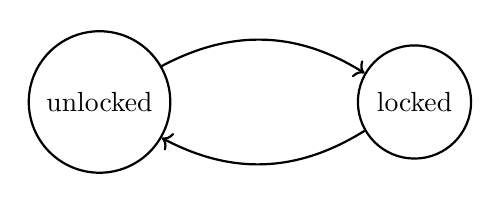
\begin{tikzpicture}[term/.style={circle,draw,thick,minimum size=8mm,inner sep=5pt},auto]
      \node (s) at (0,0) [term] {unlocked};
      \node (f) at (4,0) [term] {locked};
      \draw [->,thick] (s) to [bend left] (f);
      \draw [->,thick] (f) to [bend left] node {$\key$} (s);
    \end{tikzpicture}
  \end{center}
  The label on the transition means that the transition is only valid when we have the token $\key$, \ie{} we can only unlock a lock if we have the key.

  There are now five proof obligations, one for each of the conjuncts in the specification, and we treat each in turn.

  The first says that $\isLock(v,P,\gamma)$ is persistent, which it is
  because invariants and equality are persistent, and conjunction and
  existential quantification preserves persistency.

  The second says that $\locked(\gamma)$ \emph{is not} duplicable. This
  follows as $\key \cdot \key = \bot$ by definition of the resource algebra:
  $\ownGhost{\gamma}{\key} * \ownGhost{\gamma}{\key} \vdash
  \ownGhost{\gamma}{\key \cdot \key}$ by \ruleref{Own-op} which yields
  $\FALSE$ by \ruleref{Own-valid}. By transitivity of $\vdash$ we are
  done.

  The third is the specification of allocating a new lock, and hence needs the allocation of a lock invariant.
  We proceed to show the following triple:
  \begin{mathpar}
    \hoare{P}{\newLock ()}{v.\Exists \gamma.\isLock(v,P,\gamma)}
  \end{mathpar}
  By \ruleref{Ht-beta}, it suffices to show
  \begin{mathpar}
    \hoare{P}{\Ref(\False)}{v.\Exists \gamma.\isLock(v,P,\gamma)}
  \end{mathpar}
  We allocate new ghost state using \ruleref{Ghost-alloc}, as in Exercise~\ref{exercise:basic-properties-of-view-shift}, use the rule of consequence and then use \ruleref{Ht-exist}.
  We are left with proving
  \begin{mathpar}
    \hoare{\locked(\gamma) \ast P}{\Ref(\False)}{v.\Exists \gamma.\isLock(v,P,\gamma)}
  \end{mathpar}
  for some $\gamma$.
  \begin{exercise}
    Prove this.
    (Hint: Use the derived invariant allocation rule \ruleref{Ht-inv-alloc-post},
    and \ruleref{Ht-bind} with an empty context -).
  \end{exercise}
  
  
  The fourth is the specification of the $\acquire$ operation. It is a recursive definition, so we proceed with the derived rule for recursive functions from Exercise~\ref{exercise:derived-rule-recursive-functions}. That is, assuming 
  \begin{align}
    \All v, P, \gamma.\hoare{\later\isLock(v,P,\gamma)}{\acquire v}{\_. P \ast \locked(\gamma)}\label{eq:ih-acquire}
  \end{align}
  we show the following triple
  \begin{mathpar}
    \hoare{\isLock(v,P,\gamma)}{\If\CAS(v,\False,\True)then()\Else\acquire(v)}{\_. P \ast \locked(\gamma)}.    
  \end{mathpar}
  The $\isLock$ predicate gives us that $v$ is a location $\ell$
  governed by an invariant, which we can move into the context as follows:
  \begin{mathpar}
    \knowInv{\iota}{I(\ell,P,\gamma)}\proves
    \hoare{\TRUE}
    {\If\CAS(\ell,\False,\True)then()\Else\acquire(\ell)}
    {\_. P \ast \locked(\gamma)}
  \end{mathpar}
  We next evaluate the $\CAS$ expression with the \ruleref{Ht-bind} rule.
  As our intermediate step we proceed to show the following triple:
  \begin{mathpar}
    \knowInv{\iota}{I(\ell,P,\gamma)}\proves
    \hoare{\TRUE}
    {\CAS(\ell,\False,\True)}
    {u. (u = \True \ast  P \ast \locked(\gamma)) \lor (u = \False) }.    
  \end{mathpar}
  As $\CAS$ is atomic, we open the invariant to get at $\ell$, using
  \ruleref{Ht-inv-open}, and it suffices to show that
  \begin{mathpar}
    \knowInv{\iota}{I(\ell,P,\gamma)}\proves
    \hoareV{\later I(\ell,P,\gamma)}
    {\CAS(\ell,\False,\True)}
    {u. (\left(u = \True \ast P \ast \locked(\gamma)\right) \lor (u = \False)) \ast I(\ell,P,\gamma) }.    
  \end{mathpar}
  We proceed by cases on the invariant (using the rule \ruleref{Ht-disj}).
  In the first case we need to show
  \begin{mathpar}
    \knowInv{\iota}{I(\ell,P,\gamma)}\proves
    \hoareV{\later (\ell \pointsto \False \ast \locked{\gamma} * P)}
    {\CAS(\ell,\False,\True)}
    {u. (u = \True \ast P \ast \locked(\gamma) \lor  (u = \False)) \ast I(\ell,P,\gamma) }.
  \end{mathpar}
  By \ruleref{Ht-csq} it suffices to establish either choice of the
  disjunctions in the postcondition (there is one in the left of the
  separating conjuction, and one to the right, hidden in
  $I(\ell,P,\gamma)$).  We choose
  $u = \True \ast P \ast \locked(\gamma) * \ell\pointsto\True$ and
  by \ruleref{Ht-frame} and \ruleref{Ht-CAS-succ} we are done.
  
  In the second case, we show
  \begin{mathpar}
    \knowInv{\iota}{I(\ell,P,\gamma)}\proves
    \hoareV{\later (\ell \pointsto \True)}
    {\CAS(\ell,\False,\True)}
    {u. ((u = \True \ast P \ast \locked(\gamma) \lor
      (u = \False)) \ast I(\ell,P,\gamma) }.    
  \end{mathpar}
  Again we strengthen the post-condition, this time to
  $u = \False \ast \ell\pointsto\True$, and we are done by using the rule \ruleref{Ht-CAS-fail}.

  We are now ready to proceed with our use of \ruleref{Ht-bind}, the evaluation of the $\langkw{if}$, and the following obligation remains:
  \begin{mathpar}
    \knowInv{\iota}{I(\ell,P,\gamma)}\proves
    \hoare
    {u = \True \ast P \ast \locked(\gamma) \lor u = \False}
    {\If u then ()\Else\acquire\ell}
    {\_.P * \locked(\gamma)}
  \end{mathpar}
  We consider the two cases in the precondition, using \ruleref{Ht-disj}.
  We use \ruleref{Ht-If-True} and \ruleref{Ht-If-False} in the first and second case respectively, which leaves the following two obligations:
  \begin{align*}
    \knowInv{\iota}{I(\ell,P,\gamma)}&\proves
    \hoare
    {P \ast \locked(\gamma)}
    {()}
    {\_.P * \locked(\gamma)}\\
    \knowInv{\iota}{I(\ell,P,\gamma)}&\proves
    \hoare
    {\TRUE}
    {\acquire\ell}
    {\_.P * \locked(\gamma)}       
  \end{align*}
  The first follows by the rule for the unit expressions, the second by our induction hypothesis \eqref{eq:ih-acquire}.
  This concludes the proof that $\acquire$ satisfies its specification.
    
  The fifth and final is the specification of the $\release$ operation. We proceed to show the following triple:
  \begin{mathpar}
    \hoare{\isLock(v,P,\gamma) \ast P \ast \locked(\gamma)}{\release v}{\_.\TRUE}
  \end{mathpar}
  By definition, $\isLock(v,P,\gamma)$ tells us there is a location governed by an invariant, and we can substitute this location into the expression under evaluation, and by \ruleref{Ht-beta} we can unfold the definition of $\release$:
  \begin{mathpar}
    \hoare{\knowInv{\iota}{I(\ell,P,\gamma)} \ast P \ast \locked(\gamma)}{\ell \gets \False}{\_.\TRUE}
  \end{mathpar}
  To perform the assignment we must obtain $\ell$ as a resource from the invariant, which we do by opening it with the \ruleref{Ht-inv-open} rule. As invariants are persistent, we can move it into our assumptions before opening, leaving us with the following triple:
  \begin{mathpar}
    \knowInv{\iota}{I(\ell,P,\gamma)}\vdash
    \hoare{\later I(\ell,P,\gamma) \ast P \ast \locked(\gamma)}{\ell \gets \False}{\_.\later I(\ell,P,\gamma)}
  \end{mathpar}
  We consider two cases, based on the disjunction in $I(\ell,P,\gamma)$ in the precondition.
  The first case is
  \begin{mathpar}
    \knowInv{\iota}{I(\ell,P,\gamma)}\vdash\hoare
    {\later\left(\ell \pointsto\False \ast \locked(\gamma) \ast P\right) \ast P \ast \locked(\gamma)}{\ell \gets \False}{\_.\later I(\ell,P,\gamma)}
  \end{mathpar}
  which is inconsistent as $\locked(\gamma) \ast \locked(\gamma) \vdash \FALSE$, as argued above.
  We are done by \ruleref{Ht-later-false}.
  In the second case we need to prove
  \begin{mathpar}
    \knowInv{\iota}{I(\ell,P,\gamma)}\vdash\hoare
    {\later(\ell \pointsto\True) \ast P \ast \locked(\gamma)}{\ell \gets \False}{\_.\later I(\ell,P,\gamma)}
  \end{mathpar}
  and in the postcondition we chose the first disjunct by
  \ruleref{Ht-csq} -- \ie{} we will show the following triple:
  \begin{mathpar}
    \knowInv{\iota}{I(\ell,P,\gamma)}\vdash\hoare
    {\later(\ell \pointsto\True) \ast \later(P \ast \locked(\gamma))}{\ell \gets \False}{\_.\later (\ell \pointsto \False) \ast \later(\locked(\gamma) \ast P)}
  \end{mathpar}
  which holds by the frame rule and \ruleref{Ht-store}.
\end{example}

To show how the lock specification can be used, we use it in an example program:
We implement a concurrent bag, using the spin lock to guard access to
a shared location containing the data in the bag. 

\newcommand{\isBag}{\operatorname{isBag}}
\newcommand{\baglist}{\operatorname{bagList}}
\newcommand{\newBag}{\operatorname{newBag}}
\newcommand{\binsert}{\operatorname{insert}}
\newcommand{\bremove}{\operatorname{remove}}
\newcommand{\lock}{\operatorname{lock}}

\begin{example}[Concurrent coarse-grained bag]
  \label{example:course-grained-bag}
  The implementation is as follows.
  Recall we use syntactic sugar $\None$ for $\Inj{1} \TT$ and $\Some x$ for $\Inj{2} x$.
  The $\newBag$ method allocates a new reference cell which initially contains $\None$, together with a new lock.
  This lock is used to guard access to the location in $\binsert$ and $\bremove$ methods.
  The location will always contain a list of values.
  The $\binsert$ and $\bremove$ methods insert and remove elements.
  The $\bremove$ method returns either $\None$, in the case the bag is empty, or $\Some v$, where $v$ is the head element of the non-empty list.
  \begin{align*}
    \langkw{let} \newBag = \Lam \_ . &(\Ref(\None), \newLock \TT)\\
    \langkw{let} \binsert = \Lam x . \Lam v . &\Let \ell = \Proj{1} x in\\
                                              &\Let \lock = \Proj{2} x in\\
                                              &\acquire \lock ;\\
                                              & \ell \gets \Some (v, \deref \ell) ;\\
                                              & \release \lock\\
    \langkw{let} \bremove = \Lam x . &\Let \ell = \Proj{1} x in\\
                                     &\Let \lock = \Proj{2} x in\\
                                     &\acquire \lock ;\\
                                     &\langkw{let}\ r = \MatchML{\deref \ell}with{\None}=>{\None}|{\Some p}=>{\ell \gets \Proj{2}{p} ; \Some (\Proj{1}{p})}end{} \\
                                     & \langkw{in}\ \release \lock ; r
  \end{align*}
  We would like to have a specification of the bag which will allow
  clients to use it in a concurrent setting, where different threads insert and remove elements from a bag.

  A weak, but still useful specification is the following.  Given a
  predicate $\Phi$, the bag contains elements $x$ for which $\Phi(x)$
  holds.  When inserting an element we give away the resources, and
  when removing an element we give back an element plus the knowledge
  that it satisfies the predicate.  
  The specification is:
  \begin{align*}
    &\Exists \isBag : (\Val \to \Prop) \times \Val \to \Prop.\nonumber\\
    &\All (\Phi : \Val \to \Prop).\nonumber\\
    &\quad\quad\persistently\left(\All b . \isBag(\Phi, b) \implies \persistently \isBag(\Phi,b)\right)\\
    &\land\quad\hoare{\TRUE}{\newBag \TT}{b. \isBag(\Phi,b)}\\
    &\land\quad\All b u.\hoare{\isBag(\Phi,b) \ast \Phi(u)}{\binsert b\,u}{\_.\TRUE}\\
    &\land\quad\All b.\hoare{\isBag(\Phi,b)}{\bremove b}{v.v = \None \lor \Exists x . v = \Some x \land \Phi(x)}
  \end{align*}
  With this specification, the only thing we get to know after calling
  remove is that the returned element, if we get one out, satisfies
  the chosen predicate $\Phi$.  In fact, giving a stronger
  specification is hard.  The reason is that the $\isBag$
  predicate is freely duplicable.  And we do want the $\isBag$ to be
  duplicable, since this allows us to share it between as many threads
  as we need, which in turn allows us to specify and prove concurrent
  programs.  The consequence of $\isBag$ being duplicable is that
  concurrently running threads will be able to add and remove elements, so
  each thread has no guarantee  which particular elements it will
  get back when calling $\bremove$.
  
  We now proceed to show that the implementation meets the
  specification. The $\isBag$ predicate is defined as follows:
  \begin{align*}
    \isBag(\Phi, b) = \Exists \ell v \gamma . b = (\ell, v) \land \isLock(v, \Exists xs . \ell \pointsto xs \ast \baglist(\Phi,xs), \gamma)
  \end{align*}
  where $\baglist$ is defined by guarded recursion as the unique predicate satisfying
  \begin{align*}
    \baglist(\Phi,xs) = xs = \None \lor \Exists x . \Exists r . xs = \Some (x, r) \land \Phi(x) \ast \later(\baglist(\Phi,r)).
  \end{align*}
  Let $\Phi : \Val \to \Prop$ be arbitrary.

  \begin{exercise}
    Prove that $\isBag(\Phi,b)$ is persistent for any $b$.
  \end{exercise}
  

  \begin{exercise}
    Prove the $\newBag$ specification:
    \begin{displaymath}
      \hoare{\TRUE}{\newBag \TT}{b. \isBag(\Phi,b)}.\qedhere
    \end{displaymath}
  \end{exercise}
  

  Note that since $\isBag(\Phi,b)$ is persistent for any $b$ we can derive, by using the frame rule (exercise!), the following specification
  \begin{align*}
    \All b.\hoare{\isBag(\Phi,b)}{\bremove b}{v.\left(v = \None \lor \Exists x . v = \Some x \land \Phi(x)\right) \ast \isBag(\Phi,b)}
  \end{align*}
  from the one claimed above, \ie{} we do not lose the knowledge that $b$ is a bag.

  Let us now prove the specification of the $\bremove$ method.
  We are proving
  \begin{align*}
    \hoare{\isBag(\Phi,b)}{\bremove b}{v.v = \None \lor \Exists x . v = \Some x \land \Phi(x)}
  \end{align*}
  for some value $b$.
  
  By definition of $\isBag(\Phi,b)$ and by using \ruleref{Ht-exist}, and then \ruleref{Ht-persistently} together with \ruleref{Ht-Eq} we have to prove
  \begin{align*}
    \hoare{\isLock(\lock, \Exists xs . \ell \pointsto xs \ast \baglist(\Phi,xs), \gamma)}{\bremove (\ell,\lock)}{u.u = \None \lor{} \Exists x . u = \Some x \land \Phi(x)}
  \end{align*}
  for some $\ell$, $\lock$ and $\gamma$.
  Using \ruleref{Ht-beta} and \ruleref{Ht-let-det} we reduce to showing
  \begin{align*}
    \hoare{\isLock(\lock, \Exists xs . \ell \pointsto xs \ast \baglist(\Phi,xs), \gamma)}{e}{u.u = \None \lor{} \Exists x . u = \Some x \land \Phi(x)}
  \end{align*}
  where $e$ is the program
  \begin{align*}
    &\acquire \lock ;\\
    &\langkw{let}\ r = \MatchML{\deref \ell}with{\None}=>{\None}|{\Some p}=>{\ell \gets \Proj{2}{p} ; \Some (\Proj{1}{p})}end{} \\
    & \langkw{in}\ \release \lock ; r
  \end{align*}
  Using the sequencing rule \ruleref{Ht-seq} we use the specification of $\acquire$ as the first triple, and thus we have to prove
  \begin{align*}
    \hoare{\locked(\gamma) \ast \Exists xs . \ell \pointsto xs \ast \baglist(\Phi,xs)}{e'}{u.u = \None \lor{} \Exists x . u = \Some x \land \Phi(x)}
  \end{align*}
  where $e'$ is the part of program $e$ after $\acquire$.

  Using the fact that $\exists$ and $\lor$ distribute over $\ast$ (see Figure~\ref{fig:laws-interaction-of-connectives} on page~\pageref{fig:laws-interaction-of-connectives}), \ruleref{Ht-exist} and then the definition of $\baglist(\Phi,xs)$ together with \ruleref{Ht-disj} we consider two cases.
  The first case is
  \begin{align*}
    \hoare{\locked(\gamma) \ast \ell \pointsto xs \ast xs = \None}{e'}{u.u = \None \lor{} \Exists x. u = \Some x \land \Phi(x)}
  \end{align*}
  \begin{exercise}
    Prove the above triple (possibly after looking at the proof of the second case below).
  \end{exercise}
  

  In the second case, after using rules in Figure~\ref{fig:laws-interaction-of-connectives} and \ruleref{Ht-exist}, we get the following proof obligation.
  \begin{align*}
    \hoare{\locked(\gamma) \ast \ell \pointsto xs \ast xs = \Some(x, r) \ast \Phi(x) \ast \later \baglist(\Phi,r)}{e'}{u.u = \None \lor{} \Exists x. u = \Some x \land \Phi(x)}
  \end{align*}
  which simplifies, by \ruleref{Ht-Eq} and the rule of consequence, to proving
  \begin{align*}
    \hoare{\locked(\gamma) \ast \ell \pointsto \Some(x, r) \ast \Phi(x) \ast \later \baglist(\Phi,r)}{e'}{u.\Exists x. u = \Some x \land \Phi(x)}.
  \end{align*}
  We use the let rule \ruleref{Ht-let-det}.
  For the first premise we show
  \begin{align*}
    \hoareV{\locked(\gamma) \ast \ell \pointsto \Some(x, r) \ast \Phi(x) \ast \later \baglist(\Phi,r)}{\MatchML{\deref \ell}with{\None}=>{\None}|{\Some p}=>{\ell \gets \Proj{2}{p} ; \Some (\Proj{1}{p})}end{}}{u.u = \Some x \land \ell \pointsto r \ast \Phi(x) \ast \locked(\gamma) \ast \baglist(\Phi,r)}
  \end{align*}
  (note the omission of $\later$ on $\baglist$ in the postcondition).
  We start with the bind rule, then the \ruleref{Ht-load} rule and then \ruleref{Ht-Match} which means we have to show
  \begin{align*}
    \hoareV{\locked(\gamma) \ast \ell \pointsto \Some(x, r) \ast \Phi(x) \ast \later \baglist(\Phi,r)}{\ell \gets \pi_2(x, r) ; \Some(\pi_1 (x,r))}{u.u = \Some x \land \ell \pointsto r \ast \Phi(x) \ast \locked(\gamma) \ast \baglist(\Phi,r)}
  \end{align*}
  which by using \ruleref{Ht-bind} and \ruleref{Ht-Proj} simplifies to showing
  \begin{align*}
    \hoareV{\locked(\gamma) \ast \ell \pointsto \Some(x, r) \ast \Phi(x) \ast \later \baglist(\Phi,r)}{\ell \gets r ; \Some(\pi_1 (x,r))}{u.u = \Some x \land \ell \pointsto r \ast \Phi(x) \ast \locked(\gamma) \ast \baglist(\Phi,r)}
  \end{align*}
  Using the sequencing rule we first show
  \begin{align*}
    \hoareV{\locked(\gamma) \ast \ell \pointsto \Some(x, r) \ast \Phi(x) \ast \later \baglist(\Phi,r)}{\ell \gets r }{\_. \ell \pointsto r \ast \Phi(x) \ast \locked(\gamma) \ast \baglist(\Phi,r)}
  \end{align*}
  by using \ruleref{Ht-frame-atomic} to remove the $\later$ on $\baglist$.
  The second premise of the sequence rule, the triple
  \begin{align*}
    \hoareV{\ell \pointsto r \ast \Phi(x) \ast \locked(\gamma) \ast \baglist(\Phi,r)}
    {\Some (\pi_1(x, r))}
    {u.u = \Some x \land \ell \pointsto r \ast \Phi(x) \ast \locked(\gamma) \ast \baglist(\Phi,r)}
  \end{align*}
  is then easy to establish. Exercise!

  Finally, we need to establish the second premise of the rule \ruleref{Ht-let-det}, which means showing
  \begin{align*}
    \hoareV{\ell \pointsto r \ast \Phi(x) \ast \locked(\gamma) \ast \baglist(\Phi,r)}
    {\release \lock ; \Some x}
    {u.\Exists x. u = \Some x \land \Phi(x)}
  \end{align*}
  We can use the sequencing rule together with the $\release$ specification to give away the resources $\ell \pointsto r$, $\locked(\gamma)$ and $\baglist(\Phi,r)$ back to the lock.
  We are left with proving
  \begin{align*}
    \hoareV{\Phi(x)}
    {\Some x}
    {u.\Exists x. u = \Some x \land \Phi(x)}
  \end{align*}
  which is immediate.

  \begin{remark}
    Note that even if we did not call $\release$ we could have proved the same triple, by using weakening, \ie{} the rule $P \ast Q \proves P$.
    Such an implementation would indeed be safe, but we could never remove more than one element from the bag, since we would not be able to acquire a lock more than once.
    This is a general observation about an affine program logic such as Iris.
    However in Iris it is possible to give a stronger specification to the lock module which can ensure that locks which are acquired must be released, however this requires a more sophisticated use of the Iris base logic, so we do not dwell on it here, and instead focus only on safety specifications.
  \end{remark}
  \begin{exercise}
    Prove the specification of the $\binsert$ method:
    \begin{displaymath}
      \All b u.\hoare{\isBag(\Phi,b) \ast \Phi(u)}{\binsert b\,u}{\_.\TRUE} \qedhere
    \end{displaymath}
  \end{exercise}
  
\end{example}

\subsection{Authoritative resource algebra: counter modules}
\label{sec:authoritative-ra}

\newcommand{\isCounter}{\operatorname{isCounter}}
\newcommand{\incrC}{\operatorname{incr}}
\newcommand{\readC}{\operatorname{read}}
\newcommand{\newC}{\operatorname{newCounter}}

In this section we will endeavour to specify a counter module that can be used simultaneously by many different threads.
We will see that to achieve this we will have to introduce a new kind of resource algebra, the \emph{authoritative resource algebra}.

A first attempt at a specification is as follows.
The counter module has three methods, $\newC$ for creating a fresh counter, $\incrC$ for increasing the value of the counter, and $\readC$ for reading the current value of the counter.
There is an abstract predicate $\isCounter(v,n)$ which should state that $v$ is a counter whose current value is $n$.
This predicate should be persistent, so different threads can access the counter simultaneously.
For this reason $\isCounter(v, n)$ cannot state that $n$ is \emph{exactly} the value of the counter, but only its lower bound.
The reason we can specify the lower bound is that the counter can only increase in value.
Hence in particular other threads can only increase the value of the counter, hence they can never invalidate our lower bound.

With this, the specification of the $\incrC$ method is straightforward: the lower bound of the value of the counter is increased by $1$, and moreover the increment returns the original value of the counter, of which we know the lower bound.
\begin{align*}
  \All v . \All n . \hoare{\isCounter(v, n)}{\incrC v}{u.u \geq n \ast \isCounter(v, n+1)}.
\end{align*}
Following the discussion above, when reading the value of the counter it might be larger than that known to us via the $\isCounter$ predicate, \ie{} other threads might have increased its value without us knowing it.
\begin{align*}
  \All v . \All n . \hoare{\isCounter(v, n)}{\readC v}{u.u \geq n}
\end{align*}

The counter implementation we have in mind is the following.
The $\newC$ method creates the counter, which is simply a location containing the counter value.
\begin{align*}
  \newC \TT =\ \Ref(0)
\end{align*}
The $\incrC$ method increases the value of the counter by $1$.
Since $\ell \gets \deref \ell + 1$ is not an atomic operation we use a $\CAS$ loop, as seen in examples before.
\begin{align*}
  \Rec{\incrC} \ell =\ &\Let n = \deref \ell in\\
                       &\Let m = n + 1 in\\
                       &\If \CAS(\ell, n, m) then n \Else \incrC \ell
\end{align*}
Finally the read method simply reads the value
\begin{align*}
  \readC \ell = \deref \ell.
\end{align*}

Now, what should the $\isCounter$ predicate be?
A first attempt might be simply
\begin{align*}
  \isCounter(\ell, n) = \ell \pointsto n.
\end{align*}
However this clearly cannot work, since such an $\isCounter$ predicate is not persistent.
A second attempt might be to put the points-to assertion into the invariant as
\begin{align*}
  \isCounter(\ell, n) = \Exists \iota . \knowInv{\iota}{\ell \pointsto n}.
\end{align*}
This gets us closer, but the problem is that $\ell \pointsto n$ is not an invariant of all the methods, \ie{} not all the methods maintain this invariant.
In particular the increment method does not.
Recall that we can never change the assertion stored in the invariant, \eg{} we cannot change $\knowInv{\iota}{\ell \pointsto n}$ into $\knowInv{\iota}{\ell \pointsto (n+1)}$.
An invariant would be $\Exists m . \ell \pointsto m$, but now we need to somehow relate $m$ to $n$ which is the parameter of the $\isCounter$ predicate.
An idea might be to use the invariant
\begin{align*}
  \Exists m . \ell \pointsto m \land m \geq n
\end{align*}
and thus have
\begin{align*}
  \isCounter(\ell, n) = \Exists \iota . \knowInv{\iota}{\Exists m . \ell \pointsto m \land m \geq n}.
\end{align*}
This is an invariant, however it is not strong enough.
We cannot prove the increment method using this invariant since we cannot update $\isCounter(\ell, n)$ to $\isCounter(\ell, n+1)$, because we cannot change the assertion in the invariant.
We can conclude that any attempt which mentions $n$ in the invariant directly must fail, so we need some other way to relate the real counter value $m$ and the lower bound $n$.
We will use ghost state.
The idea is that in the invariant we will have some ghost state dependent on $m$, let us call it $\ownGhost{\gamma}{\authfull m}$, whereas we will keep some other piece of ghost state in the $\isCounter(\ell, n)$ predicate outside the invariant.
Let us call this piece $\ownGhost{\gamma}{\authfrag n}$.
Let us see what we need from the resource algebra to be able to verify the counter example by using
\begin{align}
  \label{eq:iscounter-cc-reppred}
  \isCounter(\ell, n, \gamma) = \ownGhost{\gamma}{\authfrag n} \ast \Exists \iota . \knowInv{\iota}{\Exists m . \ell \pointsto m \ast \ownGhost{\gamma}{\authfull m}}
\end{align}
as the abstract predicate.
First, to verify the read method we will open the invariant, and after some simplification we will have $\ownGhost{\gamma}{\authfull m \cdot \authfrag n}$ and the value we are going to return is $m$.
From this we should be able to conclude that $m \geq n$.
Using \ruleref{Own-valid} we have $\authfull m \cdot \authfrag n \in \Vl$, where $\Vl$ is the set of valid elements of the resource algebra we are trying to define.
Hence we need to be able to conclude $m \geq n$ from $\authfull m \cdot \authfrag n \in \Vl$.
Next, if $\isCounter(\ell, n, \gamma)$ is to be persistent, it must be that $\ownGhost{\gamma}{\authfrag n}$ is persistent, which is only the case (see \ruleref{Persistently-core}) if $\mcore{\authfrag n} = \authfrag{n}$, where $\mcore{\cdot}$ is the core operation of the resource algebra we are defining.
In particular this means that $\authfrag n$ must be duplicable for any $n$.

Finally, let us see what we need to verify the $\incrC$ method.
As we have seen many times by now, we have to update the ghost state when the $\CAS$ operation succeeds.
Just before the $\CAS$ operation succeeds the following resources are available
\begin{align*}
  \ell \pointsto k \ast \ownGhost{\gamma}{\authfull k \cdot \authfrag n}
\end{align*}
and just after we will have
\begin{align*}
  \ell \pointsto (k+1) \ast \ownGhost{\gamma}{\authfull k \cdot \authfrag n}.
\end{align*}
Using these we need to reestablish the invariant, and get $\ownGhost{\gamma}{\authfrag (n+1)}$ in order to conclude
\begin{align*}
  \isCounter(\ell, n+1, \gamma).
\end{align*}
The only way to do this is to update the ghost state using \ruleref{Ghost-update}.
Thus it would suffice to have the frame preserving update
\begin{align*}
  \authfull k \cdot \authfrag n \mupd \authfull (k+1) \cdot \authfrag (n+1).
\end{align*}

To recap, here are the requirements of our resource algebra.
\begin{align}
  \label{eq:1:core-of-auth-max}
  &\mcore{\authfrag n} = \authfrag{n}\\
  \label{eq:2:valid-of-auth-max}
  &\authfull m \cdot \authfrag n \in \Vl \implies m \geq n\\
  \label{eq:3:valid-update-auth-max}
  &\authfull m \cdot \authfrag n \mupd \authfull (m+1) \cdot \authfrag (n+1)
\end{align}
We now define a resource algebra which allows us to achieve these properties.
Let $\Ml = \NN_{\bot,\top} \times \NN$ where $\NN_{\bot,\top}$ is the set of natural numbers with two additional elements $\bot$ and $\top$.
Define the operation $\cdot$ as
\begin{align*}
  (x, n) \cdot (y, m) =
  \begin{cases}
    (y, \max(n, m)) & \text{ if } x = \bot\\
    (x, \max(n, m)) & \text{ if } y = \bot\\
    (\top, \max(n, m)) & \text{ otherwise}
  \end{cases}
\end{align*}
It is easy to see (exercise!) that this makes $\Ml$ into a commutative semigroup.
Moreover it has a unit, which is the element $(\bot, 0)$.

For $m, n \in \NN$ let us write $\authfull m$ for $(m, 0)$ and $\authfrag n$ for $(\bot, n)$.
Using the definition of the operation we clearly see $\authfull m \cdot \authfrag n = (m, n)$.
Thus to get property~\eqref{eq:2:valid-of-auth-max} we should require that if $(m, n) \in \Vl$ for natural numbers $n$ and $m$ then $m \geq n$.
Moreover, the closure condition of the set of valid elements states that subparts of valid elements must also be valid.
Thus, since we wish $(n, n) = \authfrag n \cdot \authfull n \in \Vl$ we must also have $\authfrag n = (\bot, n) \in \Vl$.
With this in mind we define the set of valid elements as
\begin{align*}
  \Vl = \left\{(x, n) \isetsep x = \bot \lor x \in \NN \land x \geq n\right\}.
\end{align*}
In particular note that elements of the form $(\top, n)$ are \emph{not} valid.
With this definition we can see that property~\eqref{eq:2:valid-of-auth-max} holds.

Requirement~\eqref{eq:1:core-of-auth-max} defines the core on elements $\authfrag n$.
The only way to extend it to the whole $\Ml$ so that it still satisfies all the axioms of the core is to define
\begin{align*}
  \mcore{(x, n)} = (\bot, n).
\end{align*}
It is easy to see that this definition makes $(\Ml, \Vl, \mcore{\cdot})$ into a unital resource algebra.

Finally, let us check we have property~\eqref{eq:3:valid-update-auth-max}.
Recall Definition~\ref{def:frame-preserving-update} (on page~\pageref{def:frame-preserving-update}) of frame preserving updates.
Let $(x, y) \in \Ml$ be such that $(\authfull m \cdot \authfrag n) \cdot (x, y)$ is valid.
This means in particular that $x = \bot$ and that $m \geq \max(n, y)$.
Hence $m+1 \geq \max(n+1,y)$ and thus $(\authfull (m+1) \cdot \authfrag (n+1)) \cdot (x, y)$ is also valid, as needed.

In particular note how it was necessary that $\authfull m \cdot \authfull k = (\top, 0)$ is \emph{not} valid to conclude that $x$ must be $\bot$, which is why we define the operation in this rather peculiar way.

\begin{exercise}
  \label{exercise:simple-counter-specification}
  Let $\isCounter : \Val \to \NN \to \textlog{GhostName} \to \Prop$ be the predicate
  \begin{align*}
    \isCounter(\ell, n, \gamma) = \ownGhost{\gamma}{\authfrag n} \ast \Exists \iota . \knowInv{\iota}{\Exists m . \ell \pointsto m \ast \ownGhost{\gamma}{\authfull m}}.
  \end{align*}
  Show the following specifications for the methods defined above.
  \begin{align*}
    &\hoare{\TRUE}{\newC \TT}{u.\Exists \gamma . \isCounter(u, 0, \gamma)}\\
    &\All \gamma . \All v . \All n . \hoare{\isCounter(v, n, \gamma)}{\readC v}{u.u \geq n}\\
    &\All \gamma . \All v . \All n . \hoare{\isCounter(v, n, \gamma)}{\incrC v}{u.u \geq n \ast \isCounter(v, n+1,\gamma)} \tag*{\qedhere}
  \end{align*}
\end{exercise}


\begin{exercise}
  \label{exercise:simple-counter-spec-example-program}
  Let $e$ be the program
  \begin{align*}
    \Let c = \newC \TT in (\incrC c || \incrC c); \readC c.
  \end{align*}
  Using the specification of the counter module from the preceding exercise show the following specification for $e$.
  \begin{displaymath}
    \hoare{\TRUE}{e}{v.v \geq 1}. \qedhere
  \end{displaymath}
\end{exercise}


\subsubsection*{A more precise counter specification}

The specification of the program $e$ from the above exercise is the strongest possible given the specification of the counter from Exercise~\ref{exercise:simple-counter-specification}.
However operationally we know that the result of that program is exactly the value $2$.
With the $\isCounter$ predicate as above we cannot prove such a precise result simply because $\isCounter$ is freely duplicable, and so in each thread we do not know whether there are other threads using the counter, and thus possibly increasing its value.

In order to give a more precise specification to the counter we must keep track of whether we are the only ones who currently has access to the counter, or if there are possibly other threads using it.
This can be achieved by using fractions in the following way.
The $\isCounter$ will be parametrized by $q$ which indicates the degree of ownership of the counter.
If we own the full counter, \ie{} $q = 1$ then we know its exact value.
If we own only a part of it then we only know its lower bound.
The $\readC$ method thus has two specifications.
\begin{align*}
  &\All \gamma . \All v . \All n . \hoare{\isCounter(v, n, \gamma, {\color{red} 1})}{\readC v}{u.u = n}\\
  &\All q . \All \gamma . \All v . \All n . \hoare{\isCounter(v, n, \gamma, {\color{red} q})}{\readC v}{u.u \geq n}
\end{align*}
The increment has an analogous specification, apart from it being parametrized by $q$, and the $\newC$ method creates a counter which is owned in full by the thread that created it.

The next question is how do we share the counter.
As explained above, the $\isCounter$ predicate cannot be persistent.
Instead, when splitting the counter we must record that somebody else can also use it.
We achieve this by parameterising the counter predicate with an additional fraction $p \in (0, 1]$.
This fraction indicates our degree of knowledge about the counter.
If $p=1$ we have the full ownership of the counter, and thus can know its exact value.
Otherwise we only know its lower bound as with the previous counter specification.
By using the following splitting property of the new $\isCounter$ predicate
\begin{align*}
  \isCounter(v, n, \gamma, p) \ast \isCounter(v, m, \gamma, q) \provesIff \isCounter(v, n + m, \gamma, p + q)
\end{align*}
we can create the counter, share it among different threads, and then once all of those threads are finished executing we can combine all the counters and read off the exact value.

In light of this rule there is another way to read the assertion $\isCounter(v, n, \gamma, p)$.
We can read it as that the contribution of this thread to the total value of the counter is exactly $n$.
If $p$ is $1$ then this is the only thread, and so the value of the counter is exactly $n$.

To define the desired $\isCounter$ predicate and to prove the desired specification we will need a resource algebra similar to the one used for the first counter specification, but more involved.
To achieve it we need to generalize the resource algebra we have defined above to the construction called \emph{authoritative resource algebra}.

\begin{example}[Authoritative resource algebra]
  \label{example:authoritative-RA}
  Given a \emph{unital} resource algebra $\Ml$ with unit $\eps$, set of valid elements $\Vl$ and core $\mcore{\cdot}$, let $\authm(\Ml)$ be the resource algebra whose carrier is the set $\Ml_{\bot,\top} \times \Ml$ (recall that $\Ml_{\bot,\top}$ is the set $\Ml$ together with two new elements $\bot$ and $\top$) and whose operation is defined as
  \begin{align*}
    (x, a) \cdot (y, b) =
    \begin{cases}
      (y, a \cdot b) & \text{ if } x = \bot\\
      (x, a \cdot b) & \text{ if } y = \bot\\
      (\top, a \cdot b) & \text{ otherwise }
    \end{cases}
  \end{align*}
  The core function is defined as (recall that the core is total in a unital resource algebra; see Exercise~\ref{exercise:unital-ra-core-total})
  \begin{align*}
    \mcore{(x, a)}_{\authm(\Ml)} = \left(\bot, \mcore{a}\right)
  \end{align*}
  and the set of valid elements is
  \begin{align*}
    \Vl_{\authm(\Ml)} = \left\{(x, a) \isetsep x = \bot \land a \in \Vl \lor x \in \Ml \land x \in \Vl \land  a \mincl x\right\}
  \end{align*}
  We write $\authfull m$ for $(m,\eps)$ and $\authfrag n$ for $(\bot,n)$.
\end{example}
\begin{exercise}
  Show that the resource algebra $\Ml$ we used in the counter specification in Exercise~\ref{exercise:simple-counter-specification} is exactly the resource algebra $\authm(\NN_{\max{}})$ where $\NN_{\max{}}$ is the resource algebra whose carrier is the set of natural numbers, and its operation the maximum.
  Its core is the identity function and all elements are valid.
\end{exercise}


\begin{exercise}
  Show the following properties of the resource algebra $\authm(\Ml)$ for an arbitrary \emph{unital} resource algebra $\Ml$.
  \begin{itemize}
  \item $\authm(\Ml)$ is unital with unit $(\bot, \eps)$, where $\eps$ is the unit of $\Ml$
  \item $\authfull x \cdot \authfull y \notin \Vl_{\authm(\Ml)}$ for any $x$ and $y$
  \item $\authfrag x \cdot \authfrag y = \authfrag (x \cdot y)$
  \item $\authfull x \cdot \authfrag y \in \Vl \implies y \mincl x$
  \item if $x \cdot z$ is valid in $\Ml$ then
    \begin{align*}
      \authfull x \cdot \authfrag y \mupd \authfull (x \cdot z) \cdot \authfrag (y \cdot z)
    \end{align*}
    in $\authm(\Ml)$.
  \item if $x \cdot z$ is valid in $\Ml$ and $w \mincl z$ then
    \begin{align*}
      \authfull x \cdot \authfrag y \mupd \authfull (x \cdot z) \cdot \authfrag (y \cdot w)
    \end{align*}
    in $\authm(\Ml)$.
  \end{itemize}
\end{exercise}


Recall the $\isCounter$ predicate we used previously
\begin{align*}
  \isCounter(\ell, n, \gamma) = \ownGhost{\gamma}{\authfrag n} \ast \Exists \iota . \knowInv{\iota}{\Exists m . \ell \pointsto m \ast \ownGhost{\gamma}{\authfull m}}.
\end{align*}
We wish to incorporate into it the fraction $p$ indicating how much of the counter this thread owns.
We do this as follows.
\begin{align*}
  \isCounter(\ell, n, \gamma, p) = \ownGhost{\gamma}{\authfrag (p, n)} \ast \Exists \iota . \knowInv{\iota}{\Exists m . \ell \pointsto m \ast \ownGhost{\gamma}{\authfull (1, m)}}.
\end{align*}
Thus the invariant stores the exact value of the counter, and since it knows its exact value the fraction is $1$.
The assertion $\ownGhost{\gamma}{\authfrag (p, n)}$ connects the actual value of the counter to the value that is known to the particular thread.
Now, to be able to read the exact value of the counter when $p$ is $1$ we need the property that if $\authfull (1, m) \cdot \authfrag (1, n)$ is valid then $n = m$.
Further, we need the property that if $\authfull (1, m) \cdot \authfrag (p, n)$ is valid then $m \geq n$.
Finally, we wish to get $\isCounter(\ell, n + k, \gamma, p + q) \provesIff \isCounter(\ell, n, \gamma, p) \ast \isCounter(\ell, k, \gamma, q)$.
The way to achieve all this is to take the resource algebra $\authm\left(\left(\QQ_{01} \times \NN\right)_?\right)$ where
\begin{itemize}
\item $\QQ_{01}$ is the resource algebra of fractions from Example~\ref{example:resource-algebra-of-fractions},
\item $\NN$ is the resource algebra of natural numbers with \emph{addition} as the operation, and every element is valid,
\item and $\left(\QQ_{01} \times \NN\right)_?$ is the option resource algebra on the product of the two previous ones.
\end{itemize}

\begin{exercise}
  \label{exercise:properties-of-fractional-natural-auth-ra}
  Show the following properties of the resource algebra $\left(\QQ_{01} \times \NN\right)_?$.
  \begin{itemize}
  \item $(p, n) \cdot (q, m) = (p + q, n + m)$
  \item if $q \leq 1$ then $(p, n) \mincl (q, m)$ if and only if
    \begin{itemize}
    \item $p \leq q$ and $n \leq m$ (where $\leq$ is the standard ordering on naturals and rationals)
    \item if $p = 1$ then $q = 1$ and $n = m$.
    \end{itemize}
  \end{itemize}
  And show the following properties of the resource algebra $\authm\left(\left(\QQ_{01} \times \NN\right)_?\right)$.
  \begin{itemize}
  \item $\authfrag (p, n) \cdot \authfrag (q, m) = \authfrag(p + q, n + m)$
  \item if $\authfull (1, m) \cdot \authfrag(p, n)$ is valid then $n \leq m$ and $p \leq 1$
  \item if $\authfull (1, m) \cdot \authfrag(1, n)$ is valid then $n = m$
  \item $\authfull (1, m) \cdot \authfrag (p, n) \mupd \authfull (1, m+1) \cdot \authfrag (p, n+1)$.\qedhere
  \end{itemize}
\end{exercise}

Using the results from the preceding exercise about ghost updates the following exercise is a straightforward adaptation of Exercise~\ref{exercise:simple-counter-specification}.
\begin{exercise}
  \label{exercise:precise-counter-specification}
  Let $\isCounter$ be the predicate
  \begin{align*}
    \isCounter(\ell, n, \gamma, p) = \ownGhost{\gamma}{\authfrag (p, n)} \ast \Exists \iota . \knowInv{\iota}{\Exists m . \ell \pointsto m \ast \ownGhost{\gamma}{\authfull (1, m)}}.
  \end{align*}
  First show that for any $p, q, n$, and $k$, we have
  \begin{align*}
    \isCounter(\ell, n + k, \gamma, p + q) \provesIff \isCounter(\ell, n, \gamma, p) \ast \isCounter(\ell, k, \gamma, q).
  \end{align*}

  Next show the following specifications for the methods defined above.
  \begin{align*}
    &\hoare{\TRUE}{\newC \TT}{u.\Exists \gamma . \isCounter(u, 0, \gamma, 1)}\\
    &\All p . \All \gamma . \All v . \All n . \hoare{\isCounter(v, n, \gamma, p)}{\readC v}{u.u \geq n}\\
    &\All \gamma . \All v . \All n . \hoare{\isCounter(v, n, \gamma, 1)}{\readC v}{u.u = n}\\
    &\All p . \All \gamma . \All v . \All n . \hoare{\isCounter(v, n, \gamma, p)}{\incrC v}{u.u \geq n \ast \isCounter(v, n+1,\gamma, p)} \tag*{\qedhere}
  \end{align*}
\end{exercise}

Using the specification from the previous exercise we can now revisit Exercise~\ref{exercise:simple-counter-spec-example-program} to give it the most precise specification.
\begin{exercise}
\label{exercise:precise-counter-spec-example-program}
  Let $e$ be the program
  \begin{align*}
    \Let c = \newC \TT in (\incrC c || \incrC c); \readC c.
  \end{align*}
  Using the specification of the counter module from the preceding exercise show the following specification for $e$.
  \begin{displaymath}
    \hoare{\TRUE}{e}{v.v = 2}.\qedhere
  \end{displaymath}
\end{exercise}


\subsection{Parallel composition via \texorpdfstring{$\Fork{}$}{Fork()}}
\label{sec:parcomp-from-fork}

We can now show how to derive the proof rule \ruleref{Ht-par} which we simply stated on page~\pageref{Ht-par} from the following rule for the primitive $\Fork{}$.
The primitive $\Fork{}$ rule is as follows.
\begin{mathpar}
  \inferH{Ht-fork}
  {S \proves \hoare{P}{e}{\_.\TRUE}[\mask]}
  {S \proves \hoare{P}{\Fork{e}}{v.v = \TT}[\mask]}
\end{mathpar}
The key point is that we only require the forked-off thread to be safe, we do not care about its return value, hence the post-condition $\TRUE$ in the premise.

Recall how parallel composition is defined in Section~\ref{sec:par-construct}.
It uses two auxiliary methods $\langkw{spawn}$, which creates a new thread and a ``shared channel'' which is used to signal when it is done, and the $\langkw{join}$ method which listens on the channel until the spawned thread is done.
These methods are of independent interest since, in contrast to the plain $\Fork{}$, they allow us to wait for a forked-off thread to finish.
Since we are using a shared channel we will use an invariant to allow the two threads to access it.

The method $\langkw{spawn}$ has a function $f$ as an argument.
Let us assume that $f$ has the following specification for some predicates $P$ and $v.Q$.
\begin{align*}
  \hoare{P}{f\,\TT}{v.Q}.
\end{align*}

With these parameters fixed we define the following predicate
\newcommand{\joinH}{\operatorname{joinHandle}}
\begin{align*}
  \joinH(\ell, \gamma, v.Q) \eqdef \ownGhost{\gamma}{\TT} \ast \knowInv{\iota}{\ell \pointsto \None \lor \Exists x . \ell \pointsto \Some x \ast Q(x) \lor \ell \pointsto - \ast \ownGhost{\gamma}{\TT}}.
\end{align*}
where we are using the exclusive resource algebra over the singleton set (see Example~\ref{ex:exclusive-resource-algebra}).
The idea is that the $\langkw{spawn}$ method returns this handle, which has information about the state of the forked-off thread.
In the beginning the invariant is in the first state, with the location $\ell$ pointing to $\None$.
Once the $\langkw{spawn}$ terminates the invariant will intuitively be in the second state, with $\ell \pointsto \Some x$ and $Q(x)$.

When the $\langkw{join}$ method is waiting for the location to become $\Some x$ it will have the $\ownGhost{\gamma}{\TT}$ token, allowing it to know that the invariant is either in the first or the second state.
Once it is in the second the $\langkw{join}$ method will close the invariant in the third state, transferring $\ownGhost{\gamma}{\TT}$ into it, and obtaining $Q(x)$.

\begin{exercise}
  Following the description above show the following specifications for the $\langkw{spawn}$ and $\langkw{join}$ methods in detail.
  \begin{mathpar}
    \inferH{Ht-spawn}
    {\hoare{P}{f\,\TT}{v.Q}}
    {\hoare{P}{\langkw{spawn}(f)}{\ell.\Exists \gamma . \joinH(\ell, \gamma, v.Q)}}
    \and
    \inferH{Ht-join}
    { }
    {\hoare{\joinH(\ell, \gamma, v.Q)}{\langkw{join}(\ell)}{v.Q}}
  \end{mathpar}
  Using these specifications derive the \ruleref{Ht-par} specification of the parallel composition operation.
\end{exercise}


%%% Local Variables:
%%% mode: latex
%%% TeX-master: "../main.tex"
%%% End:


\section{Case Study: Invariants for Sequential Programs}
\label{sec:case-study:sequential-invariants}

In this section we will use a technique known as Landin's knot to define recursive functions without the use of the primitive rec f(x) = e. Instead we are going to use \emph{recursion through the store}. We first define \langkw{myrec} as: 
\begin{displaymath}
{\langkw{myrec}} \, f = 
      \Let r = \Ref(\lambda x. \, x)  in
      r \gets \left( \lambda x.\, f \, (\deref{r}) \, x \right);\ \deref{r}
\end{displaymath}

Before giving a specification to $\langkw{myrec}$ we will try to get an intuition of how Landin's knot works.
To this end we consider what a client implementing the factorial of a natural number could look like and how it would compute the factorial of $2$.
First we define the $f$ we are going to use as:
\begin{displaymath}
{\langkw{F}} = 
     \lambda f. \lambda x. \If {x = 0} then 1 \Else x * \left( f \, (x-1)\right)
\end{displaymath}
Next we define
\begin{displaymath}
{\langkw{fac}} = \langkw{myrec} \, \langkw{F}
\end{displaymath}
Hence we have that
\begin{align*}
\langkw{fac} \, 2 = \Let r = \lambda x. \, x  in r \gets \left( \lambda x. \langkw{F}\, (\deref{r})\, x\right); \ (\deref{r})\, 2 
\end{align*}
Now we consider how \langkw{fac} 2 reduces. After some steps, we have that $r \pointsto \left(\lambda x.\, \langkw{F}\,  (\deref{r})\, x\right)$ and the computation continues as
\begin{align*}
(\deref{r}) \, 2 &\stepsto \left(\lambda x.\, \langkw{F}\,  (\deref{r})\, x\right) \, 2 \\
&\stepsto  \langkw{F}\,  (\deref{r})\, 2 \\
&\stepsto \langkw{F}\,  \left(\lambda x.\, \langkw{F}\,  (\deref{r})\, x\right)\, 2 \\
&\stepsto  \lambda x. \If {x = 0} then 1 \Else x * \left( \left(\lambda x.\, \langkw{F}\,  (\deref{r})\, x\right) \, (x-1) \right)\, 2 \\
&\stepsto  \If {2 = 0} then 1 \Else 2 *  \left( \left(\lambda x.\, \langkw{F}\,  (\deref{r})\, x\right) \, (2-1) \right) \\
&\stepsto 2* \left( \left(\lambda x.\, \langkw{F}\,  (\deref{r})\, x\right) \, (2-1) \right) \\
&\stepsto 2 * \left( \left(\lambda x.\, \langkw{F}\,  (\deref{r})\, x\right) \, 1\right) \\
\vdots \\
&\stepsto 2* \If {1 = 0} then 1 \Else 1 *  \left( \left(\lambda x.\, \langkw{fac}\,  (\deref{r})\, x\right) \, (1-1) \right) \\
\vdots \\
&\stepsto 2* 1* \left( \left(\lambda x.\, \langkw{F}\,  (\deref{r})\, x\right) \, 0 \right) \\
&\stepsto 2* \left( \left(\lambda x.\, \langkw{F}\,  (\deref{r})\, x\right) \, 0 \right)\\
&\stepsto 2 * \left(\langkw{F}\,  (\deref{r})\, 0\right) \\
\vdots \\
&\stepsto 2 * \If {0 = 0} then 1 \Else 0 *  \left(\lambda x.\, \langkw{F}\,  (\deref{r})\, x\right) \, (0-1) \\
&\stepsto 2*1 \\
&\stepsto 2
\end{align*}
Now it should be clear that the trick is that $r$ is mapped to a $\lambda$-abstraction, \emph{which refers to $r$ in it's body}.
Another important observation is that the value $r$ points to never changes after it has been updated to $\lambda x.\, \langkw{F}\,  (\deref{r})\, x$ in the beginning. 

The specification we want \langkw{myrec} to satisfy is:
\begin{mathpar}
  \inferhref{Ht-myrec}{Ht-myrec}
  { \Gamma, f:\Val, g : \Val \mid S \land \All y . \All v. \hoare{P}{g v}{u.Q } \proves \All y . \All v. \hoare{P} {f\, g\, v} {u.Q}}
  { \Gamma \mid S \proves \All y . \All v. \hoare{P}{\langkw{myrec} \, f \, v}{u.Q}}
\end{mathpar}
This specification is similar to the first recursive rule from Section~\ref{sec:basic-separation-logic}. The only differences 
is that here $f$ is assumed to be a value and that we have $f\, g\, v$ in the premise instead of $e [g/f, v/x]$. 

\subsubsection*{Proof of the specification for myrec}
To prove Ht-myrec we assume the premise
\begin{align}
\label{myrec_1}
\Gamma, f:\Val, g : \Val \mid S \land \All y . \All v. \hoare{P}{g v}{u.Q } \proves \All y . \All v. \hoare{P} {f\, g\, v} {u.Q}
\end{align} 
holds.
By~\ruleref{Ht-persistently} and~\ruleref{forall-I} we have that

\begin{align}
\label{myrec_2}
\Gamma, f:\Val \mid S\proves \All g. \All y . \All v. \hoare{P \ast \left( \All y . \All v. \hoare{P}{g v}{u.Q }\right)} {f\, g\, v} {u.Q}
\end{align}
holds.

The Hoare-triple we want to prove is
\begin{align*}
\forall y, \forall v. \hoare{P}{
 \left( \lambda f. \Let r = \lambda x. \, x  in 
      r \gets \left( \lambda x.\, f \, (\deref{r})\, x \right); \ \deref{r} \right) \, f \, v
      }{u.Q}
\end{align*}
We proceed by using~\ruleref{forall-I} twice,~\ruleref{Ht-beta},~\ruleref{Ht-let},~\ruleref{Ht-frame} and \ruleref{Ht-alloc}. Hence it suffices to prove
\begin{align*}
\forall r. \hoare{\exists l. P * l=r * l \pointsto \left( \lambda x. \, x \right)}{ r \gets \left(\lambda x.\, f \, (\deref{r})\, x\right) ;\ (\deref{r}) \, v}{u.Q}
\end{align*}
By~\ruleref{forall-I},~\ruleref{Ht-exist},~\ruleref{forall-I} and~\ruleref{Ht-Pre-Eq} it suffices to show
\begin{align*}
\hoare{P * l \pointsto \left( \lambda x. \, x \right)}{ l\gets \left( \lambda x.\, f \, (\deref{l})\, x\right) ; (\deref{l})  \, v}{u.Q}
\end{align*}
Now by~\ruleref{Ht-seq},~\ruleref{Ht-frame} and~\ruleref{Ht-store} it suffices to show
\begin{align*}
\hoare{P * l \pointsto \left(\lambda x.\, f \, (\deref{l})\, x  \right)}{(\deref{l}) \, v}{u.Q}
\end{align*}
It the follows by~\ruleref{Ht-bind-det} and~\ruleref{Ht-load} that it suffices to show
\begin{align}
\hoare{P * l \pointsto \left(\lambda x.\, f \, (\deref{l})\, x  \right)}{\left(\lambda x.\, f \, (\deref{l})\, x  \right) \, v}{u.Q}
\label{myrec_lob1}
\end{align}
Thus by~\ruleref{Ht-beta},~\ruleref{Ht-bind-det} and~\ruleref{Ht-load} it suffices to show
\begin{align}
\hoare{P * l \pointsto \left(\lambda x.\, f \, (\deref{l})\, x  \right)}{f \, \left(\lambda x.\, f \, (\deref{l)}\, x  \right) v}{u.Q}
\label{myrec_lob2}
\end{align}
How do we proceed from here?

\paragraph*{First attempt -- ``Naive approach''}
Looking at triple \eqref{myrec_lob2} and comparing it to the triple at the right hand side of the $\proves$ in \eqref{myrec_1}, we see that they are similar except:
\begin{enumerate}
\item the precondition of the current triple is $P * l \pointsto \left(\lambda x.\, f \, (\deref{l})\, x  \right)$ instead of just $P$
\item in \eqref{myrec_lob2} we have $\lambda x.\, f \, (\deref{l})\, x $ instead of $g$.
\end{enumerate}

Regarding 1: As $P * l \pointsto \left(\lambda x.\, f \, (\deref{l})\, x  \right) \implies P$, it follows by~\ruleref{Ht-csq} that in order to prove a triple with precondition $P * l \pointsto \left(\lambda x.\, f \, (\deref{l})\, x  \right)$ it suffices to prove the same triple with precondition $P$ instead.

Regarding  2: As the $g$ is actually quantified by a $\forall$\footnote{see~\eqref{myrec_2}.}, we have that if we can show that $\All y . \All v. \hoare{P}{\left(\lambda x.\, f \, (\deref{l})\, x  \right) v}{u.Q }$ holds then $\hoare{P}{f \, \left(\lambda x.\, f \, (\deref{l})\, x  \right) v}{u.Q}$ follows by the assumption that~\eqref{myrec_1} holds.

Combining the two we get that it suffices to prove 
\begin{align}
\label{myrec_ht_1}
\All y . \All v. \hoare{P}{\left(\lambda x.\, f \, (\deref{l})\, x  \right) v}{u.Q }
\end{align}
We proceed by using~\ruleref{forall-I} twice and~\ruleref{Ht-beta}. It thus suffices to prove 
\begin{align*}
\hoare{P}{ f \, (\deref{l})\, v}{u.Q }
\end{align*}
Now by~\ruleref{Ht-bind} we need to show
\begin{enumerate}
\item $f \, - \, v$ is an Evaluation context.
  \label{myrec-enum-1}
\item $\hoare{P} {\deref{l}} {w. R}$
  \label{myrec-enum-2}
\item $\All w. \hoare{R}{ f \, w\, v}{u.Q }$
  \label{myrec-enum-3}
\end{enumerate}
for some $R$ of our choice. Item~\eqref{myrec-enum-1} is clear since $f$ is assumed to be a value. For item~\eqref{myrec-enum-2} we get stuck, as we no longer have $l \pointsto \left(\lambda x.\, f \, (\deref{l})\, x  \right)$ in our precondition and thus we can not dereference $l$.

\paragraph*{Second attempt -- ``L{\"o}b induction''}
In the beginning of Section~\ref{sec:introducing-later}, a fixed-point combinator for defining recursive functions was defined. In the proof of the rule for this fixed-point combinator the L{\"o}b rule played a crucial role. As we are doing something similar it might be useful to apply L{\"o}b induction here as well.

An immediate challenge is then: when should we apply the rule?
The rule needs to be applied at a stage, which we will return to later, such that we may use the assumption we get at this later time. The two best places seem to be either where we ended~\eqref{myrec_lob2}
\begin{align*}
\hoare{P * l \pointsto \left(\lambda x.\, f \, (\deref{l})\, x  \right)}{f \, \left(\lambda x.\, f \, (\deref{l})\, x  \right) v}{u.Q}
\end{align*}
or one step further back~\eqref{myrec_lob1}
\begin{align*}
\hoare{P * l \pointsto \left(\lambda x.\, f \, (\deref{l})\, x  \right)}{\left(\lambda x.\, f \, (\deref{l})\, x  \right) \, v}{u.Q}
\end{align*}
Clearly, we won't return to the exact same code later (if this was the case, then we would loop indefinitely). When we return to either of these stages, the value $v$ will be different, hence we of course want our L{\"o}b induction hypothesis to work for all values, not just a particular one. 

In the second case  this poses no problem at all; we added $v$ to the context when we used~\ruleref{forall-I} in the beginning, hence we can use~\ruleref{forall-E} before using L{\"o}b induction to get a sufficiently general assumption. 

In the first case, we can do the same trick for the value $v$ (the second argument), but we can't do so for the first argument of $f$. Looking at item~\eqref{myrec-enum-3} in our first attempt, we see that it seems likely that we would need to consider a general value for the first argument to $f$ as well.

Therefore, we decide to use L{\"o}b induction in the second case.

We start from~\eqref{myrec_lob1}. By~\ruleref{forall-E} it suffices to prove
\begin{align*}
\All v. \hoare{P * l \pointsto \left(\lambda x.\, f \, (\deref{l})\, x  \right)}{\left(\lambda x.\, f \, (\deref{l})\, x  \right) \, v}{u.Q}.
\end{align*}
Hence by L{\"o}b induction we may assume that $\later \left( \All v. \hoare{P * l \pointsto \left(\lambda x.\, f \, (\deref{l})\, x  \right)}{\left(\lambda x.\, f \, (\deref{l})\, x  \right) \, v}{u.Q}\right)$ holds.

First we get rid of the $\forall$ quantification by using~\ruleref{forall-I}. We then proceed by~\ruleref{Ht-beta},~\ruleref{Ht-bind-det} and~\ruleref{Ht-load} and thus it suffices to show
\begin{align*}
\hoare{P * l \pointsto \left(\lambda x.\, f \, (\deref{l})\, x  \right)}{f \, \left(\lambda x.\, f \, (\deref{l})\, x  \right) v}{u.Q}
\end{align*}
Now we proceed as in our first attempt. When we reach the point where we need to prove~\eqref{myrec_ht_1}, we are almost able to conclude the proof. We need to prove 
\begin{align*}
\All y. \All v.\hoare{P}{\left(\lambda x.\, f \, (\deref{l})\, x  \right) \, v}{u.Q}
\end{align*}
and we have the assumption that\footnote{Notice that the $\later$ has been stripped from the assumption we got by the L{\"o}b induction. The reason for this is that the operational semantics has taken at least one step. Concretely, one could reason as follows; the assumption is persistent, as Hoare-triples are, and since $\later$ commutes with $\persistently$. We can therefore use~\ruleref{Ht-persistently} to move the assumption into the precondition of the Hoare-triple. Each time the operational semantics takes a step, we may use~\ruleref{Ht-bind} to bind the atomic step, and then use~\ruleref{Ht-frame-atomic} to remove the $\later$ from the assumption. As the assumption without the later is still persistent, we may move it back into our assumptions by using~\ruleref{Ht-persistently} in the other direction.}
\begin{align*}
\All v. \hoare{P * l \pointsto \left(\lambda x.\, f \, (\deref{l})\, x  \right)}{\left(\lambda x.\, f \, (\deref{l})\, x  \right) \, v}{u.Q}
\end{align*}
The $\All y$ we can get rid of by~\ruleref{forall-I}, but the assumption is not strong enough, as it requires us to have $ l \pointsto \left(\lambda x.\, f \, (\deref{l})\, x  \right)$ in the precondition, which we don't have. We are thus stuck again.

If we instead had forgotten $ l \pointsto \left(\lambda x.\, f \, (\deref{l})\, x \right)$, before using L{\"o}b induction, then we would have gotten a stronger assumption that doesn't require $ l \pointsto \left(\lambda x.\, f \, (\deref{l})\, x  \right)$ to be in the precondition. Our problem would then be, that giving up $ l \pointsto \left(\lambda x.\, f \, (\deref{l})\, x  \right)$, we almost immediately get stuck:
we could go from 
\begin{align*}
\hoare{P}{\left(\lambda x.\, f \, (\deref{l})\, x  \right) \, v}{u.Q}
\end{align*}
to
\begin{align*}
\hoare{P}{f \, (\deref{l}) \, v}{u.Q}
\end{align*}
but then the loss of the right to dereference $l$ stops us from going any further.

\paragraph*{Third attempt -- ``Invariants''}

When computing the factorial of 2, we noticed that the location kept pointing to the same value after it had been initialized and updated once, i.e., that it was invariant from this point on and onwards. Let us therefore try to state this as an invariant and see how things go. For this attempt, we will try to see if we can succeed without using L{\"o}b induction. Let $\mathcal{E}$ be the current mask\footnote{We didn't explicitly annotate the Hoare-triples with masks before, as we didn't use any invariants.}.

As we have that $l \pointsto \left(\lambda x.\, f \, (\deref{l})\, x\right)$ and hence clearly $\later \left( l \pointsto \left(\lambda x.\, f \, (\deref{l})\, x \right) \right)$ it suffices by~\ruleref{Ht-inv-alloc} to prove

\begin{align*}
\Exists \iota \in \mathcal{E}.\knowInv{\iota}{l \pointsto \left(\lambda x.\, f \, (\deref{l})\, x\right)}\proves \hoare{P}{f\, \left(\lambda x.\, f \, (\deref{l})\, x  \right) v}{u.Q}[\mathcal{E}]
\end{align*}

We proceed as in the first attempt. When we get to the place, where we got stuck before, we can now use~\ruleref{Ht-bind-det} instead of \ruleref{Ht-bind}, as this time we know, what the result of dereferencing $l$ is. We thus need to show
\begin{enumerate}
\item $f \, - \, v$ is an evaluation context.
  \label{myrec-enum-inv-1}
\item $\Exists \iota \in \mathcal{E}.\knowInv{\iota}{l \pointsto \left(\lambda x.\, f \, (\deref{l})\, x\right)} \proves \hoare{P} {\deref{l}} {w. w= z \land R}[\mathcal{E}]$
  \label{myrec-enum-inv-2}
\item $\Exists \iota \in \mathcal{E}.\knowInv{\iota}{l \pointsto \left(\lambda x.\, f \, (\deref{l)}\, x\right)} \proves \hoare{R [z/ w] }{ f \, z\, v}{u.Q }[\mathcal{E}]$
  \label{myrec-enum-inv-3}
\end{enumerate}
for some $z$ and $R$ of our choice. We consider each item in turn:
\begin{enumerate}
  \item As before in the first attempt. 

  \item As $\deref{l}$ is atomic, we may use~\ruleref{Ht-inv-open} and thus it suffices to show
\begin{align*}
\Exists \iota \in \mathcal{E}.\knowInv{\iota}{l \pointsto \left(\lambda x.\, f \, (\deref{l})\, x\right)} \proves \hoareV{P \ast \later \left( l \pointsto \left(\lambda x.\, f \, (\deref{l})\, x \right) \right)} {\deref{l}} {w. w= \left( \lambda x.\, f \, (\deref{l)}\, x \right) \land R \ast \later \left( l \pointsto \left(\lambda x.\, f \, (\deref{l})\, x \right) \right)}[\mathcal{E}\setminus \{ \iota \}]
\end{align*}
Choosing $R$ to be $P$, this triple then follows by~\ruleref{Ht-frame} and~\ruleref{Ht-load}.

\item Given the choice of $R$ in item~\eqref{myrec-enum-inv-2}, the triple we need to prove is:
\begin{align*}
\Exists \iota \in \mathcal{E}.\knowInv{\iota}{l \pointsto \left(\lambda x.\, f \, (\deref{l})\, x\right)} \proves \hoare{P}{ f \, \left(\lambda x.\, f \, (\deref{l})\, x\right)\, v}{u.Q }[\mathcal{E}]
\end{align*}

Now we are stuck again. $f$ is a value and $w$ is a value, hence the next reduction step would be to apply $f$ to $w$, but we don't have any information about what then happens.
\end{enumerate}

\paragraph*{Fourth attempt -- ``Invariants + L{\"o}b induction''}
Before beginning our fourth attempt, let us try to examine our previous attempts to see if they might give any clues about how to proceed.

In the first attempt we more or less just tried to brute-force the proof; this did not work out. 

In the second attempt we tried to use L{\"o}b induction; this did not work either. The assumption, we got to deal with the recursive call was either too weak or came at the cost of the resource $l \pointsto \left(\lambda x.\, f \, (\deref{l})\, x\right)$, which was needed in order to get to the point, where the assumption had to be used.

In the third attempt, we proceeded mostly as in the first attempt, but tried to be a bit more clever by using an invariant to maintain the resource $l \pointsto \left(\lambda x.\, f \, (\deref{l})\, x\right)$. We got a bit further than in the first attempt, but we still did not have any way to deal with the recursive call.

From this it seems that we had two main challenges:
\begin{enumerate}
\item Dealing with the recursive call.
\item Maintaining the resource $l \pointsto \left(\lambda x.\, f \, (\deref{l})\, x\right)$.
\end{enumerate}
From attempt 2 it seems that L{\"o}b induction might be able to deal with the recursive call, and from attempt 3 it seems that using an invariant might be sufficient to maintain the resource. 

For our fourth attempt, we therefore decide to try using both of these techniques. Starting at the same point as in the second attempt, we have to prove

\begin{align*}
\hoare{P * l \pointsto \left(\lambda x.\, f \, (\deref{l})\, x  \right)}{\left(\lambda x.\, f \, (\deref{l})\, x  \right) \, v}{u.Q}[\mathcal{E}]
\end{align*}
First we allocate the invariant by~\ruleref{Ht-inv-alloc} and hence we need to show

\begin{align*}
\Exists \iota \in \mathcal{E}.\knowInv{\iota}{l \pointsto \left(\lambda x.\, f \, (\deref{l})\, x\right)}\proves \hoare{P}{\left(\lambda x.\, f \, (\deref{l})\, x  \right) \, v}{u.Q}[\mathcal{E}]
\end{align*}
Now we use~\ruleref{forall-E} and then L{\"o}b induction. Thus we may assume
\begin{align*}
\later \left( \All v. \hoare{P}{\left(\lambda x.\, f \, (\deref{l})\, x  \right) \, v}{u.Q}[\mathcal{E}]\right)
\end{align*}
By reasoning as in the third attempt, including opening the invariant in order to dereference $l$, we obtain that it suffices to show
\begin{align*}
\Exists \iota \in \mathcal{E}.\knowInv{\iota}{l \pointsto \left(\lambda x.\, f \, (\deref{l})\, x\right)}\proves \All y . \All v. \hoare{P}{\left(\lambda x.\, f \, (\deref{l})\, x  \right) v}{u.Q }[\mathcal{E}]
\end{align*}
This triple now follows by using~\ruleref{forall-I} to instantiate $\forall y$ and then using the assumption we got by the L{\"o}b induction. So, finally, we managed to prove the desired specification for \langkw{myrec}.

\begin{exercise}
Is it possible to prove the specification if one instead used L{\"o}b induction on the other case discussed in the second attempt? That is, can one prove
\begin{align*}
\Exists \iota \in \mathcal{E}.\knowInv{\iota}{l \pointsto \left(\lambda x.\, f \, (\deref{l})\, x\right)}\proves \All v. \hoare{P}{f\, \left(\lambda x.\, f \, (\deref{l})\, x  \right) v}{u.Q}[\mathcal{E}]
\end{align*}
under the assumption of~\eqref{myrec_1} and 
\begin{align*}
\later \left(\All v. \hoare{P}{f\, \left(\lambda x.\, f \, (\deref{l})\, x  \right) v}{u.Q}[\mathcal{E}] \right)
\end{align*}
If this is the case, then prove it.
\end{exercise}

\subsubsection*{Client: fac}
In this subsection we prove that the client \langkw{fac} does indeed compute the factorial of its argument. Recall the definition of \langkw{fac}
\begin{displaymath}
{\langkw{fac}} = \langkw{myrec} \, \langkw{F}
\end{displaymath}
where
\begin{displaymath}
{\langkw{F}} = 
     \lambda f. \lambda x. \If {x = 0} then 1 \Else x * (f \, (x-1))
\end{displaymath}
For the specification of \langkw{fac} we will use the standard mathematical definition of the factorial of a natural number:
\begin{align*}
\operatorname{factorial} \, 0 &\equiv 1 \\
\operatorname{factorial} \, (n+1)  &\equiv (n+1) * \operatorname{factorial} \, n															
\end{align*}
Now we can state the specification of \langkw{fac} as
\begin{align*}
\All n. \hoare{n \geq 0 } {\langkw{fac}\, n}{v. v =\operatorname{factorial} \, n }
\end{align*}

\paragraph*{Proof of the specification of \langkw{fac}}

Using Ht-myrec it suffices to show:
\begin{align*}
g:\Val \mid \All n. \hoare{ n\geq 0}{g\, n}{v. v =\operatorname{factorial} \, n } \proves \All n. \hoare{n \geq 0 } {\langkw{F}\, g\, n} {v. v =\operatorname{factorial} \, n }
\end{align*}
Hence we assume
\begin{align*}
\All n. \hoare{ n \geq 0}{g \, n}{v. v =\operatorname{factorial} \, n } 
\end{align*}
and then we need to show
\begin{align*}
\All n. \hoare{ n \geq 0 } {\langkw{F}\, g\, n} {v.  v =\operatorname{factorial} \, n }
\end{align*}
We proceed by using~\ruleref{forall-I} to instantiate $n$. Then we apply~\ruleref{Ht-beta} twice in order to apply \langkw{F} to its arguments. It thus suffices to prove
\begin{align*}
 \hoare{ n \geq 0} {\If {n = 0} then 1 \Else \, n\,  * \, (g \, (n-1))} {v. v =\operatorname{factorial} \, n }
\end{align*}

\begin{exercise}
Complete the proof by proving the above triple.
\end{exercise}

%%% Local Variables:
%%% mode: latex
%%% TeX-master: "../main.tex"
%%% End:


\section{Case Study: Stacks with Helping}
\label{sec:case-study:stacks-with-helping}

In this section we describe how to implement and specify a
concurrent stack with \emph{helping} (also known as
\emph{cooperation}).  This is an extended case study, and thus we do
not present proofs in detail, but only outline the arguments and
describe the important points, trusting the reader to fill in the
details.  We intend that the data structure should be useful in a
concurrent setting, and allow threads to pass data between them: some
threads may add elements and other threads might remove elements.
Therefore, the data structure does not appear as a stack, in the sense
of obeying the first-in last-out discipline, to any one
thread. Instead, from each thread's perspective the shared data
structure behaves as an unstructured bag.  From a global perspective,
the data structure behaves as a stack and, moreover, if it is only
used by one thread it behaves as a stack.  However the specification
we give in this section is only that of a bag, with elements
satisfying a given predicate.  In Section~\ref{sec:logical-atomicity}
we discuss a specification technique, which can be used to 
give a stronger specification, which allows us
to keep more precise track of the elements being pushed and
popped.\footnote{Such a stronger specification can be found in
\url{https://iris-project.org/pdfs/2017-case-study-concurrent-stacks-with-helping.pdf}.}

\newcommand{\pushS}{\ensuremath{\operatorname{push}}}
\newcommand{\popS}{\ensuremath{\operatorname{pop}}}

\paragraph*{Implementation}
The abstract data type that we are implementing is that of a stack.
Therefore, it will have two operations, $\pushS$ and $\popS$.  The
main complication of our data structure is that $\pushS$ and $\popS$
must be thread-safe.  One way to achieve this would be to use a lock
to guard access to the stack, but this is too coarse-grained and slow
when many threads wish to modify the stack concurrently.

Instead, we use a fine-grained implementation of the stack which
optimistically attempts to operate on the stack without locking and
then uses the compare and set primitive to check whether another
thread interfered -- if another thread interfered, the operation is
restarted.  If many threads operate on the stack concurrently it is
quite likely that some of them will try to push, and some of them try
to pop elements.  In such a situation we can omit actually adding the
element to a stack and instantly removing it.  We can simply pass it
from one thread to another.

This is achieved by introducing a \emph{side-channel} for threads to
communicate along.  Then, if a thread attempts to get an element from
a stack, it will first check whether the side-channel contains an
element (which will be called an \emph{offer}).  If so, it will take
the offer, but if not, the thread which wishes to get an element will
instead try to get an element from the actual stack.  A thread wishing
to push an element will act dually; it will offer its value on the
side-channel temporarily in an attempt to avoid having to compete for
the main stack.  The idea is that this scheme reduces contention on
the main atomic cell and thus improves performance.  Note that this
means that a push operation \emph{helps} a pop operation to complete
(and vice versa); hence we refer to this style of implementation as
using \emph{helping} or \emph{cooperation}.\footnote{In practise, the
  implementation of side-channels and helping is more advanced, but to illustrate
  the challenge of verifying implementations with helping, this simple
  form of helping suffices.}

\subsection{Mailboxes for Offers}
As described above we will use a side-channel in the stack implementation.
This side-channel can be implemented and specified separately, and this is what we do now.
A side-channel has the following operations:
\begin{enumerate}
\item An offer can be \emph{created} with an initial value.
\item An offer can be \emph{accepted}, marking the offer as taken and returning the underlying value.
\item Once created, an offer can be \emph{revoked} which will prevent anyone from accepting the offer and return the underlying value to the thread.
\end{enumerate}
Of course, all of these operations have to be thread-safe. That is, it
must be safe for an offer to be attempted to be accepted by multiple
threads at once, an offer needs to be able to be revoked while it is
being accepted, and so on. We choose to represent an offer as a tuple
of the actual value the offer contains and a reference to an int. The
underlying integer may take one of three values, either $0$, $1$ or
$2$. An offer of the form $(v, \ell)$ with $\ell \pointsto 0$
is the initial state of an offer, where no one has attempted to take it, nor
has it been revoked. Someone may attempt to take the offer in which
case they will use a $\CAS$ to switch $\ell$ from $0$ to $1$, leading to
the accepted state of an offer, which is $(v, \ell)$ so that
$\ell \pointsto 1$.  Revoking is almost identical but instead of
switching from $0$ to $1$, we switch to $2$.

Since both revoking and accepting an offer demand the offer to be in the initial state it is impossible for anything other than exactly one accept or one revoke to succeed.
Thus the state transition system illustrating the above protocol is as follows.
\begin{center}
  \begin{tikzpicture}[->,>=stealth',shorten >=1pt,auto,node distance=4cm,
  thick,main node/.style={circle,draw}]

  \node[main node] (1) at (0, 0)    {(-, 0)};
  \node[main node] (2) at (4,  1.0) {(-, 1)};
  \node[main node] (3) at (4, -1.0) {(-, 2)};
  \path[every node/.style={font=\small}]
  (1) edge[bend left]  node[pos=0.8, text depth=0.4cm,  left] {accept} (2)
  edge[bend right] node[pos=0.8, text depth=-0.4cm, left] {revoke} (3);
\end{tikzpicture}
\end{center}
The code of the three methods is as follows.
\newcommand{\mkoffer}{\operatorname{mk\_offer}}
\newcommand{\revoke}{\operatorname{revoke\_offer}}
\newcommand{\accept}{\operatorname{accept\_offer}}
\begin{align*}
  \mkoffer &\eqdef \lambda v. (v, \Ref(0))\\
  \revoke &\eqdef \lambda v. \begin{array}[t]{l}
                               \Let u = \Proj{1}v in\\
                               \Let s = \Proj{2}v in\\
                               \If \CAS(s, 0, 2) then \Some u \Else \None
                             \end{array}\\
  \accept &\eqdef \begin{array}[t]{l}
                    \Let u = \Proj{1}v in\\
                    \Let s = \Proj{2}v in\\
                    \If \CAS(s, 0, 1) then \Some u \Else \None
                  \end{array}
\end{align*}

The pattern of offering something, immediately revoking it, and returning the value if the revoke was successful is sufficiently common that we can encapsulate it in an abstraction called a \emph{mailbox}.
The idea is that a mailbox is built around an underlying cell containing an offer and that it provides two functions which, respectively, briefly put a new offer out and check for such an offer.
The code for this is shown below.
Note a small difference in the style from the three methods above.
When the mailbox is created it does not return the underlying store, but rather returns two closures which manipulate it.
This simplifies the process of using a mailbox for stacks where we only have one mailbox at a time, but is otherwise not an important difference.
\newcommand{\mailbox}{\ensuremath{\operatorname{mailbox}}}
\newcommand{\mbput}{\ensuremath{\operatorname{put}}}
\newcommand{\mbget}{\ensuremath{\operatorname{get}}}
\begin{align*}
  \mailbox \eqdef \lambda \_.\, &\Let r = \Ref(\None) in\\
  &\left(\left(\begin{array}{ll}
      \lambda v. &\Let \operatorname{off} = \mkoffer v in\\
                  & r \gets \Some \operatorname{off}; \revoke \operatorname{off}
    \end{array}\right),
    \left(\begin{array}{ll}
       \lambda \_.&
       \Let \operatorname{offopt} = \deref r in\\
                  &\MatchML \operatorname{offopt} with
                    \None=>\None|{\Some x}=>{\accept x}end{}
          \end{array}\right)
                    \right)
\end{align*}
We will call the first part of the tuple the $\mbput$ method, and the second one the $\mbget$ method.
Note that in a real implementation we could, depending on contention, insert a small delay between making an offer and revoking it in the $\mbput$ method so that other threads would have more of a chance to accept it.
Observe that the $\mbput$ method will return $\None$ if another thread has accepted an offer, and $\Some v$ otherwise.

\subsection{The Implementation of the Stack}
With an implementation of offers ready we can write the methods of the concurrent stack.
As described above, we will use the mailbox as the side-channel for offers.
The $\popS$ method will check whether the side-channel contains an offer using the $\mbget$ method, and the $\pushS$ method will make a temporary offer using the $\mbput$ method, and check the resulting value for whether the offer was accepted or not.
The code for the stack is as follows.
Note that this too is written in a similar style to that of mailboxes, a make function which returns two closures for the operations rather than having them separately accept a stack as an argument.
\newcommand{\stack}{\ensuremath{\operatorname{stack}}}
\begin{align*}
  \stack \eqdef \lambda \_.&\\
               &\Let \operatorname{mb} = \mailbox () in\\
               &\Let \mbput = \Proj{1}\operatorname{mb} in\\
               &\Let \mbget = \Proj{2} \operatorname{mb} in\\
               &\Let r = \Ref(\None) in\\
  &(
    \Rec{\popS} = \MatchML{\mbget ()}with{\None}=>{\MatchML{\deref r}with{\None}=>{\None}|{\Some hd}=>{\begin{array}[t]{l}
                                                                                                         \Let h = \Proj{1} hd in\\
                                                                                                         \Let t = \Proj{2} hd in\\
                                                                                                         \If \CAS(r,\Some hd,t)\\  then \Some h\\ \Else \popS \TT\end{array}}end{}}|{\Some x}=>{\Some x}end{,}\\
  &\Rec{\pushS} = 
    \MatchML{\mbput \TT}with{\None}=>{\TT}|{\Some n}=>{\begin{array}[t]{l}
                                                         \Let r' = \deref r in\\
                                                         \Let r'' = \Some (n, r') in\\
                                                         \If \CAS(r, r', r'') then \TT\\
                                                         \Else \pushS \TT
                                                       \end{array}}end{)}
\end{align*}

\subsection{A Bag Specification}

The specification of the concurrent stack only specifies the stack's behavior as a \emph{bag}, for reasons we described above.
In particular the order of insertions is not reflected in the specification.
The specification of the stack will be quite similar to the bag 
specification from Example~\ref{example:course-grained-bag}, and thus it will be parametrized by an arbitrary predicate $\Phi$.
Note that since we wrote our stack using higher-order functions, the specification of the stack method will involve nested Hoare triples, as we have seen in Section~\ref{sec:abstract-data-types}.

\begin{align*}
  \forall \Phi.\hoare{\TRUE}{\stack\TT}{p.\Exists \popS \pushS . \begin{array}{l}
                                                              p = (\popS, \pushS) \ast{}\\
                                                              \hoare{\TRUE}{\popS\TT}{v.v = \None \lor{} \Exists v' . v = \Some v' \ast \Phi(v')} \ast{}\\
                                                              \All v . \hoare{\Phi(v)}{\pushS v}{u . u = \TT \ast \TRUE}
                                                            \end{array}}
\end{align*}

Rather than directly verifying this specification, the proof depends on several helpful lemmas verifying the behavior of offers and mailboxes.
By proving these simple sublemmas, the verification of concurrent stacks can respect the abstraction boundaries constructed by isolating mailboxes as we have done.

\subsection{Verifying Offers}

The heart of verifying offers is accurately encoding the transition system described in the previous section.
Encoding this is quite similar to the encodings of transitions systems we have seen before in Section~\ref{sec:invar-ghost-state}.

Specifically, offers will be governed by a proposition
$\textlog{stages}$ which encodes what state of the three possibilities an offer is in.
Ghost state is needed to ensure that certain transitions are only possible for threads with \emph{ownership} of the offer.
To this end we use the exclusive resource algebra (Example~\ref{ex:exclusive-resource-algebra}) on the singleton set.
We write ${\exinj(())}$ for the only valid element of this resource algebra.
This element will act as a token giving the owner the right to transition from the original state to the revoked state.
The proposition encoding the transition system is
\[
  \textlog{stages}_\gamma(v, \ell) \triangleq
  (\Phi(v) \ast \ell \pointsto 0) \lor{}
  \ell \pointsto 1 \lor{}
  (\ell \pointsto 2 \ast \ownGhost{\gamma}{\exinj(())})
\]
Having defined this, the representation predicate $\textlog{is\_offer}$ is now within reach.
An offer is a pair of a location containing an integer, and a value, which is the value being offered.
Since multiple threads will share access to the offer, we use an invariant.
\[
  \textlog{is\_offer}_\gamma(v) \triangleq
  \Exists v', \ell. v = (v', \ell) \ast
  \Exists \iota. \knowInv{\iota}{\textlog{stages}_\gamma(v', \ell)}
\]
Notice that both of these propositions are parameterized by a ghost name, $\gamma$.
Each $\gamma$ should uniquely correspond to an offer and represents the ownership the creator of an offer has over it, namely the right to revoke it.
This is expressed in the specification of $\mkoffer$:
\[
  \All v. \hoare{\Phi(v)}{\mkoffer(v)}{u.\ \Exists \gamma. \ownGhost{\gamma}{\exinj(())} \ast \textlog{is\_offer}_\gamma(u)}
\]
This reads as that calling $\mkoffer$ will allocate an offer \emph{as well as} returning $\ownGhost{\gamma}{\exinj(())}$ which represents the right to revoke an offer.
The fact that $\exinj(())$ represents the right to revoke an offer can be seen in the specification for $\revoke$:
\[
  \All \gamma, v.
  \hoare{\textlog{is\_offer}_\gamma(v) \ast \ownGhost{\gamma}{\exinj(())}}
  {\textlog{revoke\_offer}(v)}
  {u . u = \None \lor{} \Exists v'. u =\Some(v') \ast \Phi(v')}
\]
The specification for $\accept$ is similar except that it does not require ownership of $\ownGhost{\gamma}{\exinj(())}$.
This is because multiple threads may call {\tt accept\_offer} even though it will only successfully return once.
\[
  \All \gamma, v.
  \hoare{\textlog{is\_offer}_\gamma(v)}
  {\textlog{accept\_offer}(v)}
  {u.u = \None \mathop{\lor} \Exists v'. u = \Some(v') \ast \Phi(v')}
\]
Proofs of these specifications are entirely straightforward based on what we have seen up until now, so we leave them to the reader.

\subsection{Verifying Mailboxes}

Having the specifications of offers in hand we can use them to give and prove specifications of the mailboxes.
Since mailbox creation returns a pair of closures, specification of mailboxes will involve nested Hoare triples.
\begin{align}
  \label{prop:spec1:mailboxspec}
  \begin{split}
    \hoare{\TRUE}{\mailbox\TT}{u. 
      \begin{array}{l}
        \Exists \mbput \mbget.\\
        u = (\mbput, \mbget) \ast{}\\
        \All v. \hoare{\Phi(v)}{\mbput(v)}{w. w = \None \lor{} \Exists v'. w = \Some(v') \ast \Phi(v')}\ast{}\\
        \hoare{\TRUE}{\mbget\TT}{w. w = \None \lor{} \Exists v'. w = \Some(v') \ast \Phi(v')}
      \end{array}}
    \end{split}
\end{align}
Note that the proof of this specification is made with no reference to the underlying implementation of offers, only to the specification described above.
Throughout the proof an invariant is maintained governing the shared mutable cell that contains potential offers.
This invariant enforces that when this cell is full, it contains an offer.
It looks like this
\[
  \textlog{is\_mailbox}(\ell) \triangleq
  \ell \pointsto \None \lor{}
  \Exists v \gamma. \ell \pointsto \Some(v) \ast \textlog{is\_offer}_\gamma(v)
\]
This captures the informal notion described above: either the mailbox is empty, or it contains an offer.
As above, we do not show a proof of the specification and leave it to the reader.

\subsection{Verifying Stacks}

We now turn to the verification of stacks themselves.
We have already given the desired specification above, but we repeat it here for the convenience of the reader.
\begin{align}
  \label{prop:spec1:stack}
  \forall \Phi.\hoare{\TRUE}{\stack\TT}{p.\Exists \popS \pushS . \begin{array}{l}
                                                              p = (\popS, \pushS) \ast{}\\
                                                              \hoare{\TRUE}{\popS\TT}{v.v = \None \lor{} \Exists v' . v = \Some v' \ast \Phi(v')} \ast{}\\
                                                              \All v . \hoare{\Phi(v)}{\pushS v}{u . u = \TT \ast \TRUE}
                                                            \end{array}}
\end{align}
Having verified mailboxes already only a small amount of additional preparation is needed before we can prove this specification.
Specifically, we need an invariant governing the shared memory cell containing the stack.
The predicate $\textlog{is\_stack}(v)$ used to form the invariant is defined as by guarded recursion as the unique predicate satisfying
\[
  \textlog{is\_stack}(v) \triangleq
  v = \None \lor{} \Exists h, t. v = \Some(h, t) \ast \Phi(h) \ast \later \textlog{is\_stack}(t)
\]
It states that all elements of the given list satisfy the predicate $\Phi$.
Having defined this, it is straightforward to define an assertion enforcing that a location points to a stack.
\[
  \textlog{stack\_inv}(\ell) \triangleq
  \Exists v'. \ell \pointsto v' \ast \textlog{is\_stack}(v')
\]
We will allocate an invariant containing this assertion during the proof of the stack specification.
With this we can now turn to proving the specification.

To start the proof we use the $\ruleref{Ht-let}$ rule 
several times, and then the 
memory allocation rule, together with the specification of mailboxes,
and thus we end up having to show
\begin{align*}
  \hoare{r \pointsto \None}{(\popS, \pushS)}{p. \Exists \popS \pushS . \begin{array}{l}
                                                              p = (\popS, \pushS) \ast{}\\
                                                              \hoare{\TRUE}{\popS\TT}{v.v = \None \lor{} \Exists v' . v = \Some v' \ast \Phi(v')} \ast{}\\
                                                              \All v . \hoare{\Phi(v)}{\pushS v}{u . u = \TT \ast \TRUE}
                                                            \end{array}}
\end{align*}
where $(\popS, \pushS)$ are the two methods in the body of the
$\stack$ method.
We should show this in a context where we have
\begin{align*}
  &\All v. \hoare{\Phi(v)}{\mbput(v)}{w. w = \None \lor{} \Exists v'. w = \Some(v') \ast \Phi(v')}\\
  &\hoare{\TRUE}{\mbget\TT}{w. w = \None \lor{} \Exists v'. w = \Some(v') \ast \Phi(v')},
\end{align*}
the specification of the mailbox.
Before verifying the specifications we allocate an invariant containing $\textlog{stack\_inv}$ which we can, since $r \pointsto \None$ implies $\textlog{stack\_inv}$.
Having done this let us verify the first method, and leave the second one for the reader.
That is, let us show
\begin{align*}
  \hoare{\TRUE}{\popS\TT}{v.v = \None \lor{} \Exists v' . v = \Some v' \ast \Phi(v')},
\end{align*}
where, of course, $\popS$ is the first method in the pair returned by
$\stack$.
Recall that we are verifying this a context with $\textlog{stack\_inv}$ and the above two specifications of $\mbput$ and $\mbget$ methods.

Since we are proving the correctness of a recursive function, we proceed by L\"ob induction, assuming
\begin{align*}
  \later\hoare{\TRUE}{\popS\TT}{v.v = \None \lor{} \Exists v' . v = \Some v' \ast \Phi(v')}.
\end{align*}
Using the specification of the $\mbget$ method we consider two cases.
If the result of $\mbget\TT$ is $\Some x$ we are done, since the specification of $\mbget$ gives us precisely what we need.
This corresponds to the fact that if an offer was made on the side-channel, then we can simply take it and we are done.
Otherwise the result of $\mbget\TT$ is $\None$ and we need to use the invariant to continue with the proof.
We thus open the invariant $\textlog{stack\_inv}$ to read $\deref r$, after which, by using the definition of the $\textlog{stack\_inv}$ predicate, we have to consider two cases.
If the stack is empty ($r \pointsto \None$) we are done, since the stack was empty, and thus we return $\None$, indicating that.
Otherwise we know $r$ pointed to a pair, where $\Phi$ holds for $h$ and $t$ satisfies $\later \textlog{stack\_inv}(t)$.
To proceed we need to open the invariant again, and after that we again consider two cases.
\begin{itemize}
\item If now $r \pointsto \None$, then $\CAS$ fails and we simply use the L\"ob induction hypothesis to proceed.
\item Otherwise, $r \pointsto \Some (h', t')$, where $\Phi(h')$ and $\later\textlog{stack\_inv}(t')$ hold.
  If the pair $(h', t')$ is equal to $(h, t)$ then $\CAS$ succeeds and we are done, since $\Phi(h)$ holds and we can close the invariant since $\textlog{stack\_inv}(t)$ holds.
  Otherwise $\CAS$ fails and we are again done by the L\"ob induction hypothesis.
\end{itemize}

%%% Local Variables:
%%% mode: latex
%%% TeX-master: "../main.tex"
%%% End:


\section{Case Study: Ticket Lock}
\label{sec:case-study:ticket-lock}

\renewcommand{\isLock}{\operatorname{isLock}}
\renewcommand{\locked}{\operatorname{locked}}
\newcommand{\issued}{\operatorname{issued}}
\renewcommand{\newLock}{\operatorname{newLock}}
\renewcommand{\acquire}{\operatorname{acquire}}
\newcommand{\wait}{\operatorname{wait}}
\renewcommand{\release}{\operatorname{release}}
\newcommand{\lockInv}{\operatorname{lockInv}}

We have seen the specification of a basic spin lock in Section \ref{sec:examples-basic-concurrency}.
However, the basic spin lock easily leads to thread starvation.
A thread can be indefinitely denied access to the critical region protected by the lock even under very strong fairness assumptions on the scheduler.
This might be acceptable in certain applications, but is undesirable in others.
A \emph{ticket lock} is a more refined spin lock which keeps track of the order in which access to critical region was demanded.
It does this by keeping two counters which represent queue positions.
The first counter is the queue position that is next in line for access to the critical region, and the second is the position of the client in the queue.
When acquiring the lock, the client first obtains a position in the queue (a \emph{ticket}) by incrementing the second counter (atomically, using the \emph{atomic fetch-and-add} operation, $\FAA$).
Then it waits until it is its turn for entering the critical region.
When releasing the lock, the first counter is incremented to allow other waiting clients to acquire the lock.

This type of lock thus behaves like a \emph{first-in first-out} queue.
This means that the threads trying to acquire the lock will be allowed to take it in the order they asked for it, or more precisely, in the order in which they obtained their tickets.
However, the specification of the ticket lock we give in this section does not express this property.
Indeed, we give the ticket lock the same specification as we gave to the spin lock in Example~\ref{ex:basic-spin-lock} on page~\ref{ex:basic-spin-lock}.
Fairness is a \emph{liveness} property, and in fact a global property of the system, \ie{} not a property of an individual method, whereas Iris -- as presented here -- only allows reasoning about safety properties.

\subsection{The atomic fetch-and-add operation}
We add an atomic fetch-and-add operation to our programming language of the form $\FAA\ \ell\ n$ where $\ell$ is a location storing an integer and $n$ is an integer.
Intuitively, this atomic operation atomically adds $n$ to the value stored in $\ell$ and returns the value stored in $\ell$ prior to the operation.
This intuition is captured in the following proof rule:
\begin{mathpar}
  \inferH{Ht-FAA}
  { }
  {\hoare{\later\ell\pointsto n}{\FAA\ \ell\ m}{u. u = n \ast \ell \pointsto (n + m)}}
\end{mathpar}

\subsection{Setup}
The ticket lock has three methods, $\newLock$ for creating a new ticket lock, and $\acquire$ and $\release$
for acquiring and releasing the lock respectively.
Moreover, we have an auxiliary $\wait$ method used by the $\acquire$ method.
In order to make the verification more readable we write it as a separate public method.
\begin{align*}
  \langkw{let} \newLock () ={} &(\Ref(0), \Ref(0))\\
  \langkw{let} \acquire l ={} &\Let o = \FAA\ (\Proj{2} l)\ 1 in \wait o \; l\\
  \langkw{let} \wait n \; l ={} &\Let o = \deref (\Proj{1} l) in \\
                           &\If{o = n}then{()}\Else{\wait n\; l}\\
  \langkw{let} \release l ={} &(\Proj{1} l) \gets \deref (\Proj{1} l) + 1
\end{align*}
As we explained above, the lock uses two mutable counters, the first for keeping track of who is currently permitted to take the lock and thereby gain access to the resources protected by it, and the second for tracking which ticket to give out to the next thread.
We will refer to them as \emph{\textbf{o}wner} and \emph{\textbf{n}ext} respectively.

In the $\acquire$ method we first try to obtain a ticket.
This is the intention of the first two lines.
However since another thread might try to obtain a ticket at the same time we need to use $\FAA$ to atomically increment to obtain a ticket in the queue.
We then proceed to wait our turn to get access to the resources protected by the lock by using the $\wait$ method.

The $\wait$ method \emph{waits} until it is the given client's turn to enter the critical region.
Note that the method does not need to use any synchronisation primitives since only the thread that acquired the lock should release it, and thus the value of $n$ will not change once it becomes $n$; this is the invariant maintained by all the methods of the ticket lock module.

Analogously, we do not need to use synchronisation primitives when releasing the lock (the $\release$ method).
Only the method which is in the critical region will increment the first counter, and thus there will be no interference between reading its value, and writing it.

As mentioned in the introduction, we can give this lock the same specification as the spin lock.
The only addition is the specification of the $\wait$ method, together with the auxiliary assertion $\issued$ used by it.
\begin{align*}
  &\Exists \isLock : \textlog{GhostName} \to \Val \to \Prop \to \Prop.\nonumber\\
  &\Exists \locked : \textlog{GhostName} \to \Prop.\nonumber\\
  &\color{red} \Exists \issued : \textlog{GhostName} \to \Val \to \Prop.\nonumber\\
  &\quad\quad\All P, v, \gamma. \isLock(v, P, \gamma) \implies \persistently \isLock(v, P, \gamma)\\
  &\land\quad\All \gamma. \locked(\gamma) \ast \locked(\gamma) \implies \FALSE\\
  &\land\quad\All \gamma. \issued(\gamma,n) \ast \issued(\gamma,n) \implies \FALSE\\
  &\land\quad\All P.\hoare{P}{\newLock ()}{v.\Exists \gamma.\isLock(v, P, \gamma)}\\
  &\color{red}\land\quad\All P, v, \gamma, n.\hoare{\isLock(v, P, \gamma) \ast \issued(\gamma, n)}{\wait (n, v)}{\_.P \ast \locked(\gamma)}\\
  &\land\quad\All P, v, \gamma.\hoare{\isLock(v, P, \gamma)}{\acquire (v)}{\_.P \ast \locked(\gamma)}\\
  &\land\quad\All P, v, \gamma.\hoare{\isLock(v, P, \gamma) \ast P \ast \locked(\gamma)}{\release (v)}{\_.\TRUE}
\end{align*}
The abstract predicate $\isLock(v, P, \gamma)$ expresses that the value $v$ (a pair of two locations) is a ticket lock protecting resources described by the predicate $P$ using the ghost resources associated with $\gamma$.
As before, the $\isLock$ predicate is persistent, so different threads can use the lock simultaneously.

We will start by defining the resource algebra, invariant, and predicates we need, and then explain our choices.
The resource algebra we use is: $\authm(\exm (\NN)_{?} \times \left(\PP_{fin} (\NN)\right)$.
All of the constructs of this RA have been previously introduced in Section~\ref{sec:ghost-state}.
The lock invariant we will use in our proof is:
\begin{align*}
  \lockInv(\gamma, \ell_{o}, \ell_{n}, P) & = \Exists o, n. \: \ell_{o} \pointsto o \ast \ell_{n} \pointsto n \ast \ownGhost{\gamma}{\authfull (o, \{ i \mid 0 \leq i < n \})}\\
  &\ast \left(\ownGhost{\gamma}{\authfrag (o, \emptyset)} \ast P \lor \ownGhost{\gamma}{\authfrag (\epsilon, \{o \})}\right).
\end{align*}
  
With this we define the $\isLock$, $\locked$ and $\issued$ predicates as follows (where $\mask$ is some chosen infinite set of invariant names)
\begin{align*}
  \isLock(v, P, \gamma) & = \Exists \ell_{o}, \ell_{n}, \iota \in \mask. v = (\ell_{o}, \ell_{n}) \ast \knowInv{\iota}{\lockInv(\gamma, \ell_{o}, \ell_{n}, P)}\\
  \locked(\gamma) & = \Exists o. \ownGhost{\gamma}{\authfrag (o, \emptyset)}\\  
  \issued(\gamma, n) & = \ownGhost{\gamma}{\authfrag (\epsilon, \{n\})}
\end{align*}

Our lock invariant keeps track of the values of the owner and next counters.
Since these change when the lock is being used, they need to be existentially quantified.
The exclusive construction in our RA expresses the fact that only one thread is allowed to take or hold the lock at any given time.
Moreover, the invariant holds an authoritative piece of ghost state, which holds both the value of the owner counter and a subset of natural numbers.
This set keeps track of which tickets have been given out.
The combination of the authoritative construction and the exclusive one is needed in order to conclude equivalent values when combining different parts of our ghost state.
The disjunction in our invariant intuitively describes whether the lock is currently acquired or not.
If the left disjunct holds then the thread with ticket number $o$ is allowed to take the lock, but has not yet done so.
This is also the reason why the lock in this case holds the predicate $P$.
If the right disjunct holds then the lock is held by the thread with ticket number $o$.

The $\locked \: (\gamma)$ predicate expresses that the lock associated with ghost name $\gamma$ is currently
locked with some ticket number.
The predicate $\issued \: (\gamma, n)$ states that ticket number $n$ has been given out.

These two predicates correspond to the two sides of the disjunction in the invariant. The intuition behind
this is that when we know either $\locked$ or $\issued$, then we can conclude that the other side of the
disjunction must currently be in the invariant, since the composition would otherwise be invalid.
    
\subsection{Proofs}
There are five proof obligations in the specification.
The first three are derived directly from the properties of the chosen resource algebra, and the definitions of the relevant predicates.
The $\isLock$ predicate is persistent since it is a separating conjunction of two persistent propositions.
The $\locked$ predicate is not duplicable due to the use of the exclusive part of our RA.
Finally, the $\issued$ predicate is not duplicable, because the composition of two sets in our RA is only valid if these sets are disjoint.

\subsubsection{newLock}
The fourth obligation is the specification for $\newLock$ and will therefore include the allocation of ghost state and the lock invariant. 
We need to show the following triple:
\begin{align*}
  \hoare{ P }{ \newLock () }{v. \Exists \gamma. \isLock (v, P, \gamma)}.
\end{align*}
By \ruleref{Ht-beta}, is suffices to show:
\begin{align*}
      \hoare{ P }{ (\Ref(0), \Ref(0)) }{v. \Exists \gamma. \isLock (v, P, \gamma)}.
\end{align*}
We first apply the \ruleref{Ht-bind-det} rule twice with $\Ref(0)$ in both cases.
We then allocate the ghost state $\ownGhost{\gamma}{(\authfull (0, \emptyset)) \cdot \authfrag (0, \emptyset)}$.
Keeping in mind that $\ownGhost{\gamma}{(\authfull (0, \emptyset)) \cdot \authfrag (0, \emptyset)} \proves \ownGhost{\gamma}{\authfull (0, \emptyset)} \ast \ownGhost{\gamma}{\authfrag (0, \emptyset)}$, we get the two pieces of ghost state we need.
Together with $P$ from the precondition and the two locations we got from the two $\Ref(0)$, we now have all the resources needed for the $\isLock$ predicate and are done.

\subsubsection{wait}
The next proof obligation is the specification for $\wait$. We want to show:
\begin{align*}
  \hoare{\isLock(v, P, \gamma) \ast \issued(\gamma, n)}{\wait (n, v)}{\_.P \ast \locked(\gamma)}
\end{align*}
This is a recursive definition, so we make use of the derived rule from Exercise~\ref{exercise:derived-rule-recursive-functions} together with the \ruleref{Ht-beta} and \ruleref{Ht-csq} rules. This means we assume:
\begin{align*}
  \hoare{\later \isLock(v, P, \gamma) \ast \later \issued(\gamma, n)}{\wait (n, v)}{\_.P \ast \locked(\gamma)}
\end{align*}
and need to show
\begin{align*}
  \hoare{\isLock(v, P, \gamma) \ast \issued(\gamma, n)}{\Let o = \deref (\Proj{1} v) in \dots}{\_.P \ast \locked(\gamma)}
\end{align*}
By unfolding the $\isLock$ predicate, we get the concrete pair of locations $\ell_{o}, \ell_{n}$ we can substitute $v$ with. Moreover, we can move our invariant into the context. We will refer to $\lockInv (\gamma, \ell_{o}, \ell_{n}, P)$ as $I$ for the remainder of the proof in order to keep the notation shorter. We now use the \ruleref{Ht-Proj} rule followed by the \ruleref{Ht-let-det} and the \ruleref{Ht-bind-det} rules with the intermediate postcondition $\{w. (w = n \ast \locked (\gamma) \ast P) \lor (w \neq n \ast \issued (\gamma, n))\}$.
So we first need to see what $\deref \ell_{o}$ evaluates to. In order to do this, we need to open our invariant with the \ruleref{Ht-inv-open} rule, since it holds the $\ell_{o} \pointsto o$ information we need. We then proceed by casing on whether $n = o$.
In the case where $n \neq o$, we need to show:
\begin{align*}
  \knowInv{\iota}{I}\proves \hoare{\later I \ast n \neq o \ast \issued(\gamma, n)}{\deref \ell_{o}}{w. ((w = n \ast \locked (\gamma) \ast P) \lor (w \neq n \ast \issued (\gamma, n))) \ast \later I}
\end{align*}
We can now use the \ruleref{Ht-load} rule and choose to prove the right side of the disjunction in the postcondition, since we directly get this information from our precondition.
In the case where $n = o$, we need to show:
\begin{align*}
  \knowInv{\iota}{I}\proves \hoare{\later I \ast n = o \ast \issued(\gamma, n)}{\deref \ell_{o}}{w. ((w = n \ast \locked (\gamma) \ast P) \lor (w \neq n \ast \issued (\gamma, n))) \ast \later I}
\end{align*}
Again we start with the \ruleref{Ht-load} rule. In this case, we need to prove the left side of the disjunction. We can now unpack $\issued$ and $I$ and replace $n$ with $o$. The composition of the different pieces of ghost state we now own is only valid if the left side of the disjunction in the precondition is currently true, i.e. we get:
$$\ell_{o} \pointsto o \ast \ell_{n} \pointsto n \ast \ownGhost{\gamma}{\authfull (o, \{ i \mid 0 \leq i < n \})} \ast \ownGhost{\gamma}{\authfrag (o, \emptyset)} \ast P \ast \ownGhost{\gamma}{\authfrag (\epsilon, \{o\})}$$
We can now reestablish the invariant, this time with the resources for the right side of the disjunction. This leaves us with:
$\ownGhost{\gamma}{\authfrag (o, \emptyset)} \ast P$, which is exactly what we need for the postcondition $\locked (\gamma) \ast P$.

The remaining proof obligation at this point is:
\begin{align*}
 \knowInv{\iota}{I}\proves \hoare{((o = n \ast \locked (\gamma) \ast P) \lor (o \neq n \ast \issued (\gamma, n)))}{\If{n = o}then{()}\Else{\wait n \; l}}{\_.P \ast \locked(\gamma)}
\end{align*}
Since our precondition is a disjunction, we will need to show the triple twice assuming the left and the right side respectively.
If we assume the left side of the disjunction we need to show:
\begin{align*}
  \knowInv{\iota}{I}\proves \hoare{o = n \ast \locked (\gamma) \ast P}{\If{n = o}then{()}\Else{\wait n \; l}}{\_.P \ast \locked(\gamma)}
\end{align*}
Since our precondition gives us the result of the if statement, we can directly use \ruleref{Ht-If-True} and notice that the postcondition follows directly from our assumptions, so we are done.
Assuming the right side, we have to show:
\begin{align*}
  \knowInv{\iota}{I}\proves \hoare{o \neq n \ast \issued (\gamma,n)}{\If{n = o}then{()}\Else{\wait n \; l}}{\_.P \ast \locked(\gamma)}
\end{align*}
Again, our precondition gives us the result to the if, so we can use the \ruleref{Ht-If-False} rule and end up with having to reason about the recursive call to $\wait$. The triple matches our outermost assumption, so we apply the induction hypothesis (\ie{} the assumption of the premise of the rule in Exercise~\ref{exercise:derived-rule-recursive-functions}) and are done.

\subsubsection{acquire}
With the specification for $\wait$ in place, we are now able to show the one for $\acquire$. We need to show the following triple:
\begin{align*}
  \hoare{\isLock(v, P, \gamma)}{\acquire (v)}{\_.P \ast \locked(\gamma)}
\end{align*}
Since $\acquire$ uses $\wait$ internally, the proof of this specification will make use of the one for $\wait$. Notice how the postconditions of both specifications are exactly the same. This means our proof intuitively consists of getting from our current precondition to the one for $\wait$ at the point where we call wait, since we can then apply its specification and be done.

We begin the same way as with $\wait$, since we are dealing with a recursive definition again. So we assume:
\begin{align*}
  \hoare{\later \isLock(v, P, \gamma)}{\acquire (v)}{\_.P \ast \locked(\gamma)}
\end{align*}
and want to show:
\begin{align*}
  \hoare{\isLock(v, P, \gamma)}{\Let o = \FAA\ (\Proj{2} v) 1 in \wait o \; v}{\_.P \ast \locked(\gamma)}
\end{align*}

By unfolding the $\isLock$ predicate, we get the concrete pair of locations $\ell_{o}, \ell_{n}$ we can substitute $v$ with. Moreover, we can move our invariant into the context. Now we use \ruleref{Ht-let-det} and \ruleref{Ht-Proj}. This means we now need to show:
\begin{align*}
  \knowInv{\iota}{\lockInv (\gamma, \ell_{o}, \ell_{n}, P)}\proves \hoare{\TRUE}{\FAA\ \ell_{n}\ 1}{o. \issued (\gamma, o)}
\end{align*}
Since $\FAA$ is atomic, we can open our invariant.
We can use the \ruleref{Ht-FAA} rule.
At this point, we obtain $\ell_{n} \pointsto n + 1$ where $n$ is the value of $\ell_{n}$ when we opened the invariant. We can now update our authoritative ghost state from $\authfull (o, \{ i \mid 0 \leq i < n \})$ to $\authfull (o, \{ i \mid 0 \leq i < n \} \cup \{n \}) \cdot \authfrag (\emptyset, \{n\})$.
Performing the union gives us exactly the resources we need to close the invariant again. Moreover, the remaining ghost state $\authfrag (\emptyset, \{n\})$ is exactly $\issued (\gamma, n)$, so we are done with the intermediate goal. At this point we need to show:
\begin{align*}
  \knowInv{\iota}{\lockInv (\gamma, \ell_{o}, \ell_{n}, P)}\proves \hoare{\issued (\gamma, n)}{\wait n \; v}{\_.P \ast \locked(\gamma)}
\end{align*}
This is exactly where we wanted to be in order to apply our $\wait$ specification, which takes care of the rest of this case.

\subsubsection{release}
The final obligation is the specification for the $\release$ method. We need to show the following triple:
\begin{align*}
      \hoare{ \isLock (v, P, \gamma) \ast \locked (\gamma) \ast P }{ \release (v) }{\_. \TRUE }.
\end{align*}
We begin with the \ruleref{Ht-beta} rule as usual. Unfolding the $\isLock$ predicate in the precondition, we get two specific locations, $\ell_{o}$ and $\ell_{n}$, and can therefore substitute $v$ for the pair of these two. Then we make use of the \ruleref{Ht-Proj} rule twice. At this point, we have to show:
\begin{align*}
      \hoare{ \lockInv (\gamma, \ell_{o}, \ell_{n}, P) \ast \locked (\gamma) \ast P }{ \ell_{o} \gets \deref \ell_{o} + 1 }{\_. \TRUE }.
\end{align*}
We now apply the \ruleref{Ht-bind-det} rule with $\deref \ell_{o}$. In
order to reason about this expression, we need the information stored in
our invariant. Since reading from a location is an atomic operation we can open our invariant at this point which will give us
\begin{align*}
\ell_{o} \pointsto o \ast \ell_{n} \pointsto n \ast \ownGhost{\gamma}{\authfull (o, \{ i \mid 0 < i \leq n \} )} \ast ((\ownGhost{\gamma}{\authfrag (o, \emptyset)} \ast P) \lor \ownGhost{\gamma}{\authfrag (\epsilon, \{o \})})
\end{align*}
for some
numbers $o$ and $n$. So we can use the \ruleref{Ht-load} rule now that
we have $\ell_{o} \pointsto o$ specifically.

Unfolding the $\locked(\gamma)$ predicate gives us $\ownGhost{\gamma}{\authfrag (o', \emptyset)}$ for some number $o'$.
Since the composition of this and the authoritative piece of ghost state must be valid, we get that $o = o'$ and we can therefore substitute one of them away.
We now close our invariant again.

We then bind $o + 1$, use the \ruleref{Ht-op} rule and are left
with showing:
\begin{align*}
      \hoare{ \lockInv (\gamma, \ell_{o}, \ell_{n}, P) \ast \ownGhost{\gamma}{\authfrag (o, \emptyset)} \ast P }{ \ell_{o} \gets (o + 1) }{\_. \TRUE }.
\end{align*}
At this point, we can open the invariant again, since storing a value is atomic. As before, this gives us access to the needed location and we can therefore use the \ruleref{Ht-store} rule. We moreover again conclude that the two $o$ values in our ghost state must be the same. Apart from this, we can see that we have $\ownGhost{\gamma}{\authfrag (o, \emptyset)}$, which means that the disjunction part of the invariant must hold $\ownGhost{\gamma}{\authfrag (\epsilon, \{ o \} )}$, since the composition would otherwise not be valid. 

At this point we can update
\begin{align*}
  \ownGhost{\gamma}{\authfull (o, \{ i \mid 0 \leq i < n \})} \cdot \ownGhost{\gamma}{\authfrag (o, \emptyset)}
\end{align*}
to
\begin{align*}
  \ownGhost{\gamma}{\authfull ((o + 1), \{ i \mid 0 \leq i < n \})} \cdot \ownGhost{\gamma}{\authfrag ((o + 1), \emptyset)},
\end{align*}
and then we can close the invariant again with these two pieces of ghost state along with $P$. 

\subsection{Discussion}
As mentioned earlier, the lock presented in this section is based on two counters.
Earlier in the notes, we have already given different specifications for counters, but rather than utilizing these, the ticket lock implementation and proof refers to the implementation of the counters. Hence it is not modular --- ideally, we should be able to verify the ticket lock relative to an abstract specification of the counter module.
This point will be addressed further in the following Section \ref{sec:modular-specs-of-concurrent-modules}.

%%% Local Variables:
%%% mode: latex
%%% TeX-master: "../main.tex"
%%% End:


\section{Case study: The Array-Based Queueing Lock}
\label{sec:array-lock}

\newcommand{\addition}[1]{\textcolor{red}{ #1 }}

\newcommand{\seq}{\text{seq}}

\renewcommand{\Cap}{\textit{cap}\xspace}
\newcommand{\Rem}{\ensuremath{\;\mathrm{rem}\;}}
\newcommand{\Div}{\ `\text{div}`\ }
\newcommand{\length}{\text{length}\xspace}

\newcommand{\allocN}{\langkw{alloc$_N$}}
\newcommand{\plusl}{+_{l}}

% Multi letter math variables we use
\newcommand{\Array}{\textit{array}\xspace}
\newcommand{\xs}{\textit{xs}\xspace}
\newcommand{\ps}{\textit{ps}\xspace}
\newcommand{\ticket}{\textit{ticket}}
\newcommand{\Next}{\textit{next}}

\newcommand{\lockedGKO}{\text{locked}(\gamma, \kappa, o)}
\newcommand{\isLockA}{\ensuremath{\isLock(\gamma, \iota, \kappa, l, \Cap, R)}\xspace}
\newcommand{\invitation}{\operatorname{invitation}}
\newcommand{\issuedA}{\text{issued}(\gamma, o)}
\newcommand{\rightK}{\ensuremath{\text{right}(\kappa)}\xspace}
\newcommand{\leftK}{\ensuremath{\text{left}(\kappa)}\xspace}
\newcommand{\bothK}{\ensuremath{\text{both}(\kappa)}\xspace}
\newcommand{\nthTrue}{\text{nthTrue}}
\newcommand{\nthTrueCapO}{\text{nthTrue}(\Cap, o \Rem \Cap)}

\renewcommand{\Prop}{\textsf{Prop}}
\renewcommand{\Val}{\text{Val}}
\newcommand{\GN}{\textsf{GhostName}} % GhostName
\newcommand{\replicate}{\operatorname{replicate}}

% Language keywords
\newcommand{\true}{\textsf{true}}
\newcommand{\false}{\textsf{false}}

\newcommand{\arraylock}{array-based queuing lock\xspace}

The array-based queuing lock (ABQL) is a lock closely related to the ticket
lock. The cache behaviour of the ABQL scales better to a large number of threads
at the cost of increased space usage and of only being safe with a bounded
number of concurrent threads. The latter must be modelled when proving safety of
the lock, and hence the ABQL poses unique and interesting challenges to such
efforts.

In this section we describe the \arraylock{} and its implementation in
\proglang. As we have done for the other locks, we then give and prove a
specification which shows that the ABQL is safe, and hence that it satisfies
mutual exclusion.

\subsection{Arrays in \proglang} \label{sec:array}

As the name of the \arraylock{} implies, its implementation relies on arrays. We
therefore first introduce how arrays are supported in \proglang{}.

One may wonder why arrays are necessary, given that we have already seen how
lists can be implemented in \proglang. The key difference is that arrays offer
constant time random-access to elements in the array. In addition to the
performance benefits of this, it also means that reading and writing elements in
an array is an atomic expression.

We need to be able to create arrays of a given size, access elements in an array
at a specific index, and update values at an index in an array. To this end
\proglang{} includes the following syntactic constructs:
\begin{displaymath}
  \begin{array}{lrcl}
    & \binop & \bnfdef{} & \cdots \ALT \plusl
    \\
    \Expr \quad
    & \expr & \bnfdef{} & \cdots
                          \ALT \allocN(e, e)
    \\
    \ECtx\quad
    & E & \bnfdef{}& \cdots
                     \ALT \allocN(E, e)
                     \ALT \allocN(v, E)
    \\
  \end{array}
\end{displaymath}

In order to express that a location $\ell$ points to an array corresponding to a
list $v$, we use the predicate $\ell \pointsto_{*} v$ with the typing rule
\begin{mathpar}
  \infer{\vctx \proves \wtt{\ell}{\Val} \and \vctx \proves \wtt{v}{\mathrm{list}\ \Val}}
  {\vctx \proves \wtt{\ell \pointsto_{*} v}{\Prop}}
\end{mathpar}

If $n$ is a number and $v$ is a value, then $\allocN(n, v)$ represents the
allocation of an array that is $n$ long and which is initialized with the value
$v$ at every index. We use $\replicate(n, v)$ to denote a mathematical list
consisting of the value $v$ repeated $n$ times. The behavior of $\allocN$ is
then captured by the following rule:
\begin{mathpar}
    \inferH{Ht-allocN}
    { }
    { S \proves \hoare{\TRUE}{\allocN(n, v)}{w . \Exists \ell . w = \ell\land \ell \pointsto_{*} \replicate(n, v)}}
\end{mathpar}
To index into an array the $\plusl$ operator is used. If $\ell$ points to the
start of an array then $\ell \plusl i$ is a location pointing to the value of
the $i$'th element, counting from $0$. If $\xs$ is a mathematical list, we use the notation
$xs_{i}$ to denote the $i$'th entry in the list.
\begin{mathpar}
    \inferH{Ht-load-offset}
    { }
    { S \proves
      \hoare{ \ell \pointsto_{*} \xs \ast \xs_i = e }
            { \deref (\ell \plusl i) }
            {v. v = e \land \ell \pointsto_{*} \xs }}
\end{mathpar}
To update an element in an array we use the store operator in combination with
$\plusl$.
\begin{mathpar}
    \inferH{Ht-store-offset}
    { }
    { S \proves \hoare{ \ell \pointsto_{*} \xs \land n < \length(\xs)}{(\ell \plusl n) \gets v}{v. v = \TT \land \ell \pointsto_{*} \xs[n := v] }}
\end{mathpar}
The operator $\plusl$ can be thought of as pointer arithmetic and then this way
of using arrays is similar to how arrays are implemented in many low-level
programming languages. Handling arrays in this manner in Iris has the benefit
that we only need to add $\plusl$ and can reuse the load and store operators in
the context of arrays.

\subsection{The implementation}
\label{sec:arraylock}

Having seen how arrays work, we now describe the ABQL and present an
implementation in \proglang.

The lock consists of a natural number \textit{next} and an array of booleans
\textit{array}. The number represents the next ticket available and the array
contains \False{} at every entry, except for one, which contains \True{}. The
\emph{index} of the \True{} value in the array represents which ticket currently
grants access to the lock.

Constructing an ABQL takes as argument a natural number \Cap{}, specifying the
capacity of the lock. An array of length \Cap{} is then initialized with \True{}
at the first entry and \False{} at all other entries. The natural number which
represents the next ticket is initially set to 0.

To acquire the lock, a ticket is received using \FAA. The primitive \FAA{}
atomically returns the number stored at a location and adds a number to the stored
value. The received ticket, modulo the capacity of the lock, is an index into
the array. By spinning on the value at this index in the array until it becomes
\True{}, the lock is acquired.

To release the lock, the entry corresponding to the ticket from which the lock
was acquired is updated from \True{} to \False. Then, the next index in the
array, modulo \Cap, is set to \True. This signals to the next thread that it can
acquire the lock.

In the implementation we use a triple to represent the lock. We use $(-, -, -)$
as notation for $((-, -), -)$ and abuse notation slightly by letting $\Proj1$,
$\Proj2$, and $\Proj{3}$ denote the projections of a triple denoted in this
manner. The first element in the triple is the array, the second the
\textit{next} number, and the third is the length of the array, which we store
since arrays in \proglang{} do not have a length operation. The implementation
is then:
\begin{align*}
  \langkw{let} \newLock \Cap = \ & \Let \Array = \allocN(\False,\ \Cap) in \\
                                 & (\Array \plusl 0) \gets \True; \\
                                 & (\Array,\ \Ref(0),\ \Cap) \\
  \langkw{let} \acquire\ l =\ &\Let \Next = \Proj2\ l in \\
                                 & \Let \ticket = \FAA\ \Next\ 1 in \\
                                 & \wait l\ \ticket; \\
                                 & \ticket \\
  \langkw{let} \wait l\ t =\ &
                               \Let \Array = \Proj1\ l in \\
                                 & \Let i = t \Rem (\Proj{3}\ l) in \\
                                 & \If \deref (\Array \plusl i) then () \Else (\wait l\ t) \\
  \langkw{let} \release\ l\ o =\ & \Let \Array = \Proj1\ l in \\
                                 & \Let \Cap = \Proj{3}\ l in \\
                                 & \Array \plusl (o \Rem \Cap) \gets \False ; \\
                                 & \Array \plusl (o + 1 \Rem \Cap) \gets \True
\end{align*}

\subsection{The specification}

The specification can be seen as an extension of the specification for the
ticket lock. The significant changes specific to the ABQL are highlighted in red
in the presentation below.
\begin{align*}
  & \exists \isLock : \GN \to \GN \to \GN \to Val \to \nat \to \Prop \to \Prop. \\
  & \exists \locked : \GN \to \GN \to \Prop. \\
  & \exists \issued : \GN \to \nat \to \Prop. \\
  & \addition{\exists \invitation : \GN \to \nat \to \nat \to \Prop.} \\
  & \quad\quad \forall \gamma, \iota, \kappa, l, \Cap, R.\ \isLockA \Rightarrow \persistently \isLockA \\
  & \color{red} \land\quad \forall \iota, n, m, \Cap.\ \invitation(\iota, n, \Cap) \ast \invitation(\iota, m, \Cap)
       \Leftrightarrow \invitation(\iota, n + m, \Cap) \\
  & \land\quad \forall \Cap, R.\ \hoare{ R \ast \addition{0 < \Cap} }
      { \newLock \addition{\Cap} }
      { l.\ \Exists \gamma, \iota, \kappa. \isLockA \ast \addition{\invitation(\iota, \Cap, \Cap) }} \\
  & \land\quad \forall \gamma, \iota, \kappa, l, \Cap, R.\ \hoare{ \isLockA \ast \addition{\invitation(\iota, 1, \Cap)} }
      { \acquire\ l }
      { \addition{o}.\ \locked(\gamma, \kappa, \addition{o}) \ast R }  \\
  & \land\quad \forall \gamma, \iota, \kappa, l, \Cap, R.\ \hoare{ \isLockA \ast \issued(\gamma, t) }
      { \wait l\ t}
      { \_.\ \locked(\gamma, \kappa, t) \ast R } \\
  & \land\quad \forall \gamma, \iota, \kappa, l, \Cap, R.\ \hoare{ \isLockA \ast \lockedGKO \ast R }
      { \release\ l\ o }
      { \_.\ \addition{\invitation(\iota, 1, \Cap)} }
\end{align*}
The $\isLockA$ predicate represents the knowledge that the value $l$ is a lock
with a capacity of \Cap, and which protects the resource $R$. Since the lock is
supposed to be used in a concurrent setting the \textit{isLock} predicate is
persistent, as we have seen before.
The predicates $\lockedGKO$ and $\issued(\gamma, t)$ serve the same
purpose as they did in the ticket lock.

The precondition for \textit{newLock} requires that a lock must be created with
a capacity greater than zero. This is required as the implementation performs
modulo with \Cap, which is not defined for zero.

The biggest change is the addition of \textit{invitations}. Since every thread
waiting to acquire the lock is spinning on an entry in the array, and since the
array is \Cap long, at most \Cap{} threads may simultaneously attempt to acquire
the lock.

The predicate $\invitation(\iota, n, \Cap)$ denotes the ownership of $n$
invitations where $\Cap$ invitations exists in total. When the lock is created,
$\Cap$ invitations are also constructed, see
the postcondition for $\newLock$. In order to acquire the lock, one invitation
is required and is surrendered to the lock. When a thread later releases the lock, an
invitation is given back, as seen in the postcondition for $\release$, such that
the thread can then acquire the lock again.

Since invitations are not duplicable, we ensure that at most $\Cap$ threads
can simultaneously attempt to acquire the lock. Invitations can be split
and combined, meaning that the ownership of $n + m$ invitations implies the
separate ownership of $n$ and $m$ invitations.

\subsection{Representing invitations with ghost state}

The invitation predicate is implemented as ghost state using the following
resource algebra. We define the carrier of the resource algebra as
\[
  \mathcal{M} = (\nat \times \nat) \cup \bot.
\]
The first number in the pair represents how many invitations are owned, and the
second how many invitations exist in total.

It should not be possible to have more invitations than the total number of
invitations, and hence the valid elements are defined as
\[
\mathcal{V} = \{ (n,m) \mid n \leq m \}.
\]

Since it should be possible to combine and separate invitations, we define the
operation as
\begin{align*}
  (a, n) \cdot (b, m) =
    \begin{cases}
      (a + b, m) & \text{ if } n = m \\
      \bot & \text{ otherwise }
    \end{cases}.
\end{align*}
It only makes sense to combine invitations with the same upper bound, and hence
the operation returns $\bot$ if the two upper bounds are not equal. Invitations
should not be duplicable, and to this end the core function is
always undefined.

With this resource algebra in place, we now define invitations as
\[
  \invitation(\gamma, a, n) = \ownGhost{\gamma}{(a, n)}.
\]

\begin{exercise}
  Show that the resource algebra defined above satisfies the requirements
  given in the definition of a resource algebra
  (Definition~\ref{def:resource-algebra}).
\end{exercise}


\subsection{Implementation of the specification}
\label{sec:implementation-spec}

Having understood the purpose of invitations we are now ready to show that the
implementation meets the specification. We adopt the notation $\seq(o, i)$ for the
set of numbers $\{ n \in \nat \mid o \leq n < o + i \}$ and define the following
predicates:
\begin{align*}
  \isLockA =& \ 
     \Exists a, n, \delta \in \varepsilon. \\
        & \quad l = (a, n, \Cap)\ \ast 0 < \Cap\ \ast \\
        & \quad \knowInv{\delta}{\lockInv(\gamma, \iota, \kappa, a, \Cap, n, R)} \\
  \lockInv(\gamma, \iota, \kappa, a, \Cap, n, R) =& \
    \Exists o, i, xs. \\
        & \quad n \gmapsto (o + i) \ \ast a \gmapsto_{*} xs \ast \length\ \xs = \Cap\ \ast \\
        & \quad \invitation(\iota, i, \Cap) \ast \ownGhost{\gamma}{\authfull ( o, \seq(o, i))} \ast \\
        & \quad \text{state}(\gamma, \kappa, \Cap, o, R, xs) \\
  \text{state}(\gamma, \kappa, \Cap, o, R, xs) =&\ 
        (\ownGhost{\gamma}{\circ (o, \emptyset)} \ast R \ast \bothK \ast xs = \nthTrueCapO) \lor \\
        & \ (\issuedA \ast \rightK \ast xs = \replicate(\false, \Cap)) \lor \\
        & \ (\issuedA \ast \leftK \ast xs = \nthTrueCapO) \\
  \issued(\gamma, t) =&\ \ownGhost{\gamma}{\circ(\munit, \{ t \})} \\
  \lockedGKO =&\ \ownGhost{\gamma}{\circ(o, \emptyset)} \ast \rightK
\end{align*}
In the following subsections we describe these predicates
at a high-level and identify several useful
and central properties as lemmas, which we then refer back to when we present the proofs.
Hopefully this makes it easier for the reader to understand how the various
pieces fit together.

\subsubsection{The ghost state}

The ghost state with ghost name $\gamma$ is defined using the resource algebra
$\authm(\exm(\nat)_{?} \times (\mathbb{P}_{\textit{fin}}(\nat)))$. This is the
same resource algebra used in the ticket lock. Intuitively, an element of this
resource algebra is a pair where the first element can include knowledge about
the value of $o$, which represents that the thread with this ticket currently
has or may acquire the lock, and the second element knowledge about which tickets currently
exist.

We use \emph{disjoint} union such that partial knowledge about the existence
of a ticket can only exist once. Hence we have the following lemma:
\begin{lemma} \label{prop:issuedcontra}
  Only a single thread can know that a certain ticket has been issued.
  \[ \ownGhost{\gamma}{\circ(\munit, \{ t \})} \ast \ownGhost{\gamma}{\circ(\munit, \{ t \})} \wand \bot \]
\end{lemma}
Similarly, the exclusive construct around the value of $o$ ensures that this information can also only exist once.
\begin{lemma} \label{prop:knowocontra}
  Only a single thread can have the partial information about $o$.
  \[ \ownGhost{\gamma}{\circ(o, \emptyset)} \ast \ownGhost{\gamma}{\circ(o, \emptyset)} \wand \bot \]
\end{lemma}

The predicates \textit{left}($\kappa$), \textit{right}($\kappa$), and \textit{both}($\kappa$)
are defined using the
resource algebra $\exm(\unitty)_{?} \times \exm(\unitty)_{?}$ where $\unitty$ denotes
the unit resource algebra with the single element \unittt:
\begin{align*}
    \leftK = \ownGhost{\kappa}{(\unittt, \munit)} \quad \quad
    \rightK = \ownGhost{\kappa}{(\munit, \unittt)} \quad \quad
    \bothK = \ownGhost{\kappa}{(\unittt, \unittt)} .
\end{align*}

\begin{lemma} \label{prop:leftrighcombine}
The resource \bothK splits into \leftK and \rightK, and \leftK and \rightK can be combined back together into \bothK.
\begin{align*}
  \bothK \ \wand \ \leftK \ast \rightK \\
  \leftK \ast \rightK \  \wand \ \bothK
\end{align*}
\end{lemma}
\begin{lemma} \label{prop:bothnocombine} Any other combination of $\leftK$,
  $\rightK$, and $\bothK$ except for those in Lemma~\ref{prop:leftrighcombine}
  is invalid.
\end{lemma}
Both lemmas follow directly from the definition of the resource algebra and the
rules \ruleref{Own-op} and \ruleref{Own-valid}.

\subsubsection{The \textit{isLock} predicate}

The \textit{isLock} predicate states the existence of $a$, which is the array
value, and $n$ which is a location pointing to the index of the next ticket. The
equality $l = (a, n, \Cap)$ describes the physical representation of the lock.
The inequality $ 0 < \Cap $ serves to constrain \Cap such that we can use it to
do division with remainder. Finally, \textit{isLock} contains the invariant
which we describe in the next subsection.

\subsubsection{The invariant}

The invariant \textit{lockInv} states the existence of three things. A natural number $o$,
representing that the thread with this ticket currently has or may acquire the
lock. The number $i$, which represents how many threads are currently waiting to
acquire the lock. Finally, $\xs$ is a list of booleans corresponding to the
current contents of the array.

The invariant contains the points-to predicate for $n$ (from the \textit{isLock} predicate)
\[
  n \gmapsto o + i.
\]
As one would expect, $n$ points to the ticket currently granting access to the
lock added together with the number of threads waiting for the lock.

Inside the invariant we have the authoritative part
\[
  \ownGhost{\gamma}{\authfull ( o, \seq(o, i))}.
\]
The lock always knows the value of $o$ and of all the tickets in existence. Here
we have made an important change compared to the equivalent part in the ticket
lock. In the ticket lock the set of tickets always starts from 0, and it is only
expanded when new tickets are issued. In some sense, tickets are not ``cleaned
up'' after their usage. For the ABQL it is important that the set of tickets
starts at $o$. This means that whenever $o$ increases, we know that all tickets
smaller than $o$ no longer exist. Hence, we have the following lemma.
\begin{lemma} \label{prop:ticketbound}
  From $\issuedA$ and the content of the invariant one can conclude $o \leq t < o + i$.
  More precisely,
  \[
    \ownGhost{\gamma}{\circ(\munit, \{ t \})} \ast \ownGhost{\gamma}{\authfull(o, \seq(o, i))}
    \wand
    \ownGhost{\gamma}{\circ(\munit, \{ t \})} \ast \ownGhost{\gamma}{\authfull(o, \seq(o, i))}
    \ast o \leq t < o + i.
  \]
\end{lemma}
The lemma is straightforward to show. Suppose the two ghost states are owned. By
\ruleref{Own-op} and \ruleref{Own-valid} the product of the two elements of the
resource algebra is also owned and is valid. From the definition of the
authoritative resource algebra and the disjoint set resource algebra this
implies $ \{ t \} \subseteq \seq(o, i) $. Which per the definition of
\textit{seq} means that we have the bound in the lemma. This tighter bound is
not needed for the proofs of the ticket lock to go through but for the ABQL it
is necessary.

The invariant also contains ghost state for invitations, which we have already
described. It is used as \[ \invitation(\iota, i, \Cap) \] inside the invariant.
This establishes the connection that $i$ is the number of invitations owned by
the lock. If $i$ threads are currently waiting for the lock then $i$ invitations
are currently owned by the lock. This corresponds to the specification where,
when calling \textit{acquire}, a thread surrenders an invitation and when
calling \textit{release} the invitation is handed back. In the meantime the
invitation is ``stored'' in the lock. As discussed previously the inclusion of
invitations serves to constrain how many threads can wait for the lock. Indeed
we have the following key property:
\begin{lemma} \label{prop:iLtCap}
The $\invitation(\iota, i, \Cap)$ in the invariant establishes the inequality $i \leq \Cap$.
\[\invitation(\iota, i, \Cap) \wand i \leq \Cap \]
\end{lemma}
This lemma follows from the definition of invitation, \ruleref{Own-valid}, and
the definition of validity of the resource algebra. This lemma is essential when
proving the specification for \textit{wait}.

\subsubsection{The \textit{state} of the lock}

The $\text{state}(\gamma, \kappa, \Cap, o, R, xs)$ disjunction represents the
current state of the lock. The first disjunct corresponds to the lock being
\textit{open} and the disjunct includes resource $R$ since the lock owns the
resource in this state. The last disjunct corresponds to the lock being
\textit{closed}. We call the middle disjunct \textit{clopen}. It is necessary,
since the release function proceeds in \emph{two} atomic steps when it reopens
the lock. Between these two steps the lock is neither closed nor open. Hence
this disjunction is crucial in the proof of release.
\begin{center}
  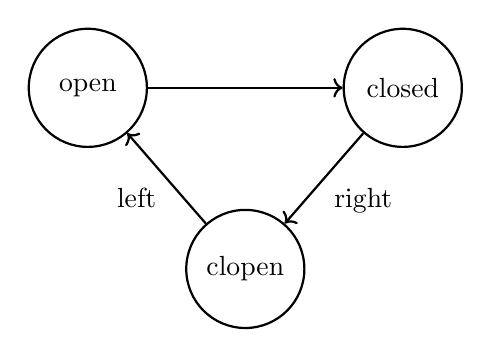
\begin{tikzpicture}[term/.style={circle,draw,minimum size={1.5cm},inner sep=5pt},auto]
    \node [thick] (o) at (0, 0) [term] {open};
    \node [thick] (c) at (4, 0) [term] {closed};
    \node [thick] (cl) at (2,-2.3) [term] {clopen};
    \draw [->,thick] (o) to node {} (c);
    \draw [->,thick] (c) to node {right} (cl);
    \draw [->,thick] (cl) to node {left} (o);
  \end{tikzpicture}
\end{center}
In the first and third disjunct $\nthTrueCapO$ denotes a mathematical sequence
of booleans of length \Cap with \False{} at every index except for index $o
\Rem \Cap$ which contains \True.

\subsubsection{The \textit{issued} token}

The $\issued(\gamma, t)$ token represents the information that the ticket $t$
has been issued. The key property of this token is that if the resource
$\issuedA$ is owned then it is possible to conclude that the lock is open.
\begin{lemma} \label{prop:issuedopen}
  Owning $\issuedA$ is sufficient to conclude that the lock is open.
  \[
\issuedA \ast \text{state}(\gamma, \kappa, \Cap, o, R, xs) \wand
        (\ownGhost{\gamma}{\circ (o, \emptyset)} \ast R \ast \bothK \ast xs = \nthTrueCapO)
  \]
\end{lemma}
This follows since $\issuedA$ is incompatible with itself per
Lemma~\ref{prop:issuedcontra} which leads to a contradiction in the
\textit{clopen} and \textit{closed} branch of the \textit{state} disjunction.

\subsubsection{The \textit{locked} predicate}

The $\lockedGKO$ predicate represents the knowledge that the lock is currently locked
along with the knowledge of what $o$ actually is. The ghost state \rightK is
included such that it is possible to conclude that the lock is in the
\textit{locked} state. This holds since the \textit{open} state contains
$\bothK$ and the \textit{clopen} state contains \rightK, both of which
contradicts with $\rightK$ per Lemma~\ref{prop:bothnocombine}.
\begin{lemma}
  From $\lockedGKO$ it is possible to conclude that the lock is closed.
  \[
    \lockedGKO \ast \text{state}(\gamma, \kappa, \Cap, o, R, xs) \wand \issuedA \ast \leftK \ast xs = \nthTrueCapO
  \]
\end{lemma}

\subsection{Proofs}
\label{sec:proofs}
We now prove the specification for each of the functions.

\subsubsection{Proof of newLock}

We sketch the proof of \textit{newLock} only at a high level as it is fairly
trivial. After executing the $\allocN$ and writing \True{} at the first index
with $(\Array \plusl 0) \gets \True$ we know that the returned value represents
an array with \True{} at index zero and \False{} at all other indices. We can
then establish the \textit{isLock} predicate by supplying a matching sequence of
booleans as a witness. For $n$ we supply the witness $0$. We must then allocate
an invariant and the ghost state it requires. Both of these can be done with the
appropriate allocation rules and by framing. When establishing the
\textit{state} disjunction in the invariant, we show the disjunct corresponding
to the lock being open.

\subsubsection{Proof of acquire}

For the \textit{acquire} function we must prove the following specification:
\[
\hoare{ \isLockA \ast \invitation(\iota, 1, \Cap) }
      { \acquire\ l }
      { o.\ \lockedGKO \ast R }
\]
Recall that the function is defined by the following \proglang code.
\begin{align*}
\langkw{let} \acquire\ l =\ &\Let \Next = \Proj2\ l in \\
    & \Let \ticket = \FAA\ \Next\ 1 in \\
    & \wait l\ \ticket; \\
    & \ticket
\end{align*}
From the \textit{isLock} predicate we know that $l$ is a triple and that there exists a location $n$ which is the second element of the triple.
Using these facts and structural rules we can step through the projection and the first \textsf{let}-expression.
We now apply the bind rule on the expression $\FAA\ n\ 1$. Since $\FAA$ is an
atomic expression we can open the lock invariant. From opening the lock
invariant we know that there exists natural numbers $o$ and $i$ such that $n$
points to $o + i$. With this points-to predicate, we can apply the
\textsc{Ht-faa} rule after which we know
\[
  n \gmapsto o + i + 1
\]
and that the $\FAA\ n\ 1$ expression evaluates to the value $o + i$.

We must now close the invariant, which per the definition means that we have to
show:
\begin{align*}
\Exists o, i, xs.
    & n \gmapsto (o + i) \ \ast a \gmapsto_{*} xs \ast \length\ \xs = \Cap\ \ast
    \invitation(\iota, i, \Cap) \ast \\
    & \ownGhost{\gamma}{\authfull ( o, \seq(o, i))} \ast
     \text{state}(\gamma, \kappa, \Cap, o, R, xs)
\end{align*}
The only part of the invariant we no longer have is $n \gmapsto o + i$. Instead,
we now have $n \gmapsto o + i + 1$. Thus, when we close the invariant we have to
provide either $o + 1$ as a witness for $o$ or $i + 1$ as a witness for $i$.
Since $o$ represents the index of who may currently access the lock and $i$
represents how many threads are waiting, it only makes sense to increment $i$.
Hence, we provide $o$ as a witness for $o$ and $i + 1$ as a witness for $i$. For
\xs we provide the same value we got when opening the invariant. Since we only
changed $i$ we can frame away the part of the invariant that does not depend on
$i$. The points-to assertion $n \gmapsto o + i + 1$ can also be framed away
since we picked $i$ exactly such that it matched the points-to assertion we had
after the fetch-and-add.

In order to close the invariant we are now left with showing
\[
  \invitation(\iota, i + 1, \Cap) \ast \ownGhost{\gamma}{\authfull(o, \seq(o, i + 1)}.
\]
From opening the invariant we have $\invitation(\iota, i, \Cap)$ and from the
precondition in the specification we have $\invitation(\iota, 1, \Cap)$. We can
combine these two facts to get $\invitation(\iota, i + 1, \Cap)$ and frame the
same thing away in the postcondition.

To show the second item we must update the authoritative ghost state we got when
opening the invariant, namely $\authfull(o, \seq(o, i))$. We can update it to
$\authfull(o, \seq(o, i) \cup \{ o + i \}) \mtimes \circ(\munit, \{ o + i \})$.
The first part of the product is exactly what we need to close the invariant,
and the second is $\issued(\munit, o + i)$ which we will need later when calling
\textit{wait}.

After closing the invariant we can evaluate the let-expression and are then left with
\begin{align*}
  & \wait l\ (o + i); o + i
\end{align*}
Since the code is a sequencing of two expressions we apply the sequencing rule.
We have the \textit{isLock} predicate, $\issued(\munit, o + i)$, and the code
$\wait l\ (o + i)$. This is fits the $\wait$ specification, which we apply. The
postcondition for the specification gives us the resource $R$ and
$\locked(\gamma, \kappa, o + i)$. Additionally, the last expression evaluates to
$o + i$. This matches precisely with the postcondition for the specification,
and we are done by framing.

\subsubsection{Proof of wait}

We now prove the specification for the \textit{wait} function.
\[
\hoare{ \isLockA \ast \issued(\gamma, t) }
      { \wait l\ t}
      { \_.\ \locked(\gamma, \kappa, t) \ast R }.
\]
Recall that the implementation of \textit{wait} is.
\begin{align*}
\langkw{let} \wait l\ t =\ &
      \Let \Array = \Proj1\ l\ in \\
    & \Let i = t \Rem (\Proj{3}\ l) in \\
    & \If \deref (\Array \plusl i) then () \Else (\wait l\ t)
\end{align*}

The definition is recursive, so we apply the \ruleref{Ht-Rec} rule, and assume
that the specification holds for any recursive call.

From the \textit{isLock} predicate we know that $l$ is a triple and that there
exists a value $a$, which is the first element of the triple, and a natural
number $\Cap$, which is the third element of the triple. With this information we
can step through the projections and the \textsf{let}-expressions. We then focus on
the condition 
\begin{equation*}
     \deref (\Array \plusl i)
\end{equation*}
with the bind rule.
We now open the invariant which contains the information that there exists an
$\xs$ such that $\Array \gmapsto_{*} \xs$. In order for the expression to make
sense, the index must be smaller than the length of the array. Fortunately, we
know from the invariant that the length of the array is $\Cap$ and $t \Rem \Cap$
is certain to be smaller than $\Cap$. From this we can show that the load
expression evaluates to a boolean $b$ where
\begin{equation} \label{eq:bvalue}
 b = \xs_{(t \Rem \Cap)}
\end{equation}
Since $b$ is a boolean it is either true or false, and we proceed by case
analysis on $b$.

We first consider the case where $b = \false$ as it is the simplest case.
It suffices to show:
\begin{align*}
     & \If \False then () \Else (\wait l\ t)
\end{align*}
We cannot step forward through the code until after we close the invariant. We
still have everything from opening the invariant, so we simply use the exact same
values as witnesses to close the invariant. We then apply \ruleref{Ht-If-False}
which leaves us with the code
\begin{align*}
   \wait l\ t
\end{align*}
This is a recursive call of \textit{wait} and we can now apply the
specification we assumed when we used the \ruleref{Ht-Rec} rule earlier. This
concludes the first case.

In the second case we have $b = \true$. Intuitively, we are in this case because
the lock is open. Not only is the lock open, our ticket $t$ should be equal to
the ticket which now grants access to the lock, namely $o$. If we can show this,
then we have $\issuedA$, and we can then use Lemma~\ref{prop:issuedopen} to
conclude that the lock is open.

Consider the $\text{state}(\gamma, \kappa, \Cap, o, R, xs)$ part of the
invariant:
\begin{align*}
        & (\ownGhost{\gamma}{\circ (o, \emptyset)} \ast R \ast \bothK \ast xs = \nthTrueCapO) \lor \\
        & (\issuedA \ast \rightK \ast xs = \replicate(\false, \Cap)) \lor \\
        & (\issuedA \ast \leftK \ast xs = \nthTrueCapO).
\end{align*}

The second case of the disjunction contains the equality
\begin{align*}
  \xs = \replicate(\false, \Cap)
\end{align*}
This states that $\xs$ is a list containing only \false. This is a
contradiction, as we have just read $\true$ at an index in the array. In
particular, we know that $b = \true$ and $b = \xs_{(t \Rem \Cap)}$. It is easy
to show that $\xs = \replicate(\false, \Cap)$ implies that $\xs_i = \false$ for
any $i$ smaller than $\Cap$. And, since $t \Rem \Cap$ is certainly smaller than
$\Cap$ we have the desired contradiction.

Both of the remaining cases contains the equality $\xs = \nthTrueCapO$.
Combining this with Equation \ref{eq:bvalue} we get
\[
  \nthTrueCapO_{(t \Rem \Cap)} = \true.
\]
Recall that $\nthTrueCapO$ denotes a list that only contains \true{} at index $o \Rem \Cap$.
Thus the above implies
\begin{equation} \label{eq:otremeq}
  o \equiv t \quad (\text{mod } \Cap).
\end{equation}
This is, unfortunately, not enough to prove $t = o$. It could, for instance,
still be the case that $t = o - \Cap$ or $t = o + \Cap$. However, considering
how the ABQL works neither of these can actually happen.
\begin{itemize}
  \item We can never have a ticket that is smaller than $o$. Then it would
    already have been our turn to acquire the lock.
  \item Our ticket can not be larger than $o + \Cap$. Intuitively, $t - o$
    represents how many threads are currently in front of us in the queue to
    acquire the lock. But, because at most $\Cap$ threads can ever wait for the
    lock, our position in the queue can be no larger than $\Cap$.
\end{itemize}
Fortunately, both of these intuitions are encoded in the definitions and can be
shown as follows.

We have $\issued(\gamma, t) = \ownGhost{\gamma}{\circ(\munit, \{ t \})}$ and
$\ownGhost{\gamma}{\authfull(o, \seq(o, i)}$. By using
Lemma~\ref{prop:ticketbound} we have
\[
  o \leq t < o + i
\]
This shows the first item above, that $t$ can not be smaller than $o$.

From opening the invariant we have 
$\invitation(\iota, i, \Cap)$. We can thus use Lemma~\ref{prop:iLtCap} to
conclude that $i \leq \Cap$. Put together with the above, we have the second
item.
\[ t < o + i \leq o + \Cap. \] This is sufficient to show that $t = o$. We leave
the details as an exercise.
\begin{exercise}
  Show that given $\Cap, t, o \in \mathbb{Z}$ where $0 < \Cap$ and $o \leq t < o
  + \Cap$ the equality $t \Rem \Cap = o \Rem \Cap$ implies that $ t = o $.
\end{exercise}


This means that in both of the remaining cases we have $\issued(\gamma, o)$ and
per Lemma~\ref{prop:issuedcontra} we now know that the lock must be in the
state corresponding to open.

In other words, from opening the lock invariant we now also have $\bothK$, the resource $R$, and the partial information $\ownGhost{\gamma}{\circ(o, \emptyset)}$.
We can split $\bothK$ into a $\leftK$ and a $\rightK$.
This means that we have $\issued(\gamma, o)$, $\leftK$, and, from opening the invariant, $xs = \nthTrueCapO$.
These are exactly the things needed to show the \textit{closed} state of the disjunction in the invariant.
Thus we can close the invariant providing the same variables we initially got for $o$, $i$, and $\xs$ followed by framing.

We have now closed the invariant and can step further into the code. We use the
\ruleref{Ht-If-True} rule and are left with
\[
  ()
\]
Hence, the only thing left to show is the postcondition. This includes $R$ and
$\lockedGKO = \ownGhost{\gamma}{\circ(o, \emptyset)} \ast \rightK$. Both of
these follow from framing as we have these from the invariant.

\subsubsection{Proof of release}

In this section we describe the proof of the specification for the
\textit{release} function. Recall the specification:
\[
\hoare{ \isLock(\gamma, \iota, \kappa, l, \Cap, R) \ast \locked(\gamma, \kappa, o) \ast R }
      { \release\ l\ o }
      { \_.\ \invitation(\iota, 1, \Cap) }
\]
Also recall that \textit{release} is defined as follows.
\begin{align*}
  \langkw{let} \release\ l\ o =\ & \Let \Array = \Proj1\ l in \\
                                 & \Let \Cap = \Proj{3}\ l in \\
                                 & \Array \plusl (o\ `rem`\ \Cap) \gets \False ; \\
                                 & \Array \plusl (o + 1\ `rem`\ \Cap) \gets \True
\end{align*}
We can evaluate the two let expressions using the facts from the isLock
predicate which leaves us with
\begin{align*}
  & \Array \plusl (o\ `rem`\ \Cap) \gets \False ; \\
  & \Array \plusl (o + 1\ `rem`\ \Cap) \gets \True
\end{align*}

Before we proceed any further, let us take a step back and consider how the proof
must proceed. In the code above, there are two store operations that write into
the array. Since the points-to predicate for the array is inside the invariant
we must open the invariant twice. Each time we open the invariant we must
consider the state$(\gamma, \kappa, \Cap, o, R, \xs)$ disjunction inside the
invariant.

Since the lock is closed when we open the invariant for the first time, we
should be able to conclude that it is in the \textit{closed} state. We then set
the single \True{} value in the array to \False. Hence, we must close the
invariant in the \textit{clopen} state. When we open the invariant for the
second time, we should be able to conclude that the disjunction is still in the
\textit{clopen} state. Finally, after the last store operation we should be able
to close the invariant in the \textit{open} state.

We use the bind rule to focus on the first store operation.
\begin{align*}
  \Array \plusl (o\ `rem`\ \Cap) \gets \False
\end{align*}
We now open the invariant and get the existence of $o'$, $i$, and \xs such that
\begin{align*}
  & n \gmapsto (o' + i) \ast
    \Array \gmapsto_{*} \xs \ast \length\ \xs = \Cap \ast \\
  & \invitation(\iota, i, \Cap) \ast
    \ownGhost{\gamma}{\authfull ( o', \seq(o', i))} \ast
    \text{state}(\gamma, \kappa, \Cap, o', R, xs)
\end{align*}
Since we have $\rightK$ we can conclude that the $\text{state}(\gamma, \kappa,
\Cap, o', R, xs)$ disjunction is in the last state as the first branch contains
$\bothK$ and the second branch contains $\rightK$---both of which lead to a
contradiction when combined with $\rightK$. We therefore additionally know.
\[
  \text{issued}(\gamma, o') \ast \leftK \ast \xs = \nthTrue(\Cap, o' \Rem \Cap).
\]
When closing the invariant we want to show the middle part of the state
disjunction, and hence our goal is to show
\[
  \text{issued}(\gamma, o') \ast \rightK \ast \xs = \replicate(\false, \Cap).
\]
The only thing we must work for is $\xs = \replicate(\false, \Cap)$ as the
other properties can be framed away. Fortunately, this is exactly what we
expect to be able to show after stepping through the store as this operation is
supposed to overwrite the single \True{} in the array with a \False. But, notice
that we are setting the array using the value $o$, but, that the information
from the invariant describes where the \True{} value is in the list in terms of
$o'$. We therefore want to show that $o$ and $o'$ are in fact equal. To do
this we combine $\ownGhost{\gamma}{\circ(o, \emptyset)}$ from the
$\locked(\gamma, \kappa, o)$ predicate in the precondition with 
$\ownGhost{\gamma}{\authfull ( o', \seq(o', i))}$ from the invariant.

We now have $ \xs = \nthTrue(\Cap, o' \Rem \Cap)$ and the code
\begin{align*}
  \Array \plusl (o\ `rem`\ \Cap) \gets \False
\end{align*}
From this we can show the postcondition $\xs = \replicate(\false, \Cap)$.
This is what we need to close the invariant in the \textit{clopen} state.
We frame everything else away.

We now focus on the next store operation. We still have the resources we started
with except that instead of \rightK we now have \leftK, and the code is
\begin{align*}
  \Array \plusl (o + 1\ `rem`\ \Cap) \gets \True
\end{align*}
We again open the invariant. Similarly to how we previously used \rightK to
determine the state of the disjunction in the lock we now use \leftK to
determine that the lock is still in the clopen state. We therefore have $\xs =
\replicate(\false, \Cap)$ and $\Array \gmapsto \replicate(\false, \Cap)$. After
executing the store operation we thus have
\[
  \Array \gmapsto \nthTrue(\Cap, (o + 1) \Rem \Cap)
\]
We are now ready to close the invariant for the last time.
When closing the invariant in the open state we must provide three witnesses and show the following.
\begin{align*}
  \Exists o, i, xs. & n \gmapsto (o + i) \ \ast a \gmapsto_{*} xs \ast \length\ \xs = \Cap\ \ast \\
    & \invitation(\iota, (i - 1), \Cap) \ast \ownGhost{\gamma}{\authfull ( o, \seq(o, i))} \ast \\
    &  \ownGhost{\gamma}{\circ (o, \emptyset)} \ast R \ast \bothK \ast xs = \nthTrueCapO
\end{align*}
For $o$ we provide $o + 1$, since we have now effectively moved the \true{}
value in the array one element to the left. For $\xs$ we provide
$\nthTrue(\Cap, (o + 1) \Rem \Cap)$. When we opened the invariant every entry in
\xs{} was \false{} but we have updated one entry to \true. For $i$ we provide
$i - 1$. We do this because invariant contains $n \gmapsto o + i$ and since we
are providing $o + 1$ in the place of $o$ we have to establish
$n \gmapsto (o + 1) + i$. But, we have not changed what $n$ points to so we
still only have $n \gmapsto o + i$. The only way we can make this work is to use
$i - 1$ as the witness for $i$.

With this choice of witnesses we can immediately frame away $R$ and the
points-to predicate for the array. The equality involving the length is
trivially true. We show \bothK{} by combining the \leftK{} and the \rightK{}
that we have with \ruleref{Own-op} followed by framing.

For the points-to predicate we have $n \gmapsto o + i$ and are to show
$n \gmapsto o + 1 + (i - 1)$. Since we are working with natural numbers
$(o + 1) + (i - 1)$ is only equal to $o + i$ if $i$ is greater than 0. We thus
have the points-to predicate if we can show that $i$ is greater than 0.

From opening the invariant we have both
$\issuedA = \ownGhost{\gamma}{\circ(\munit, \{o\})}$ and
$\ownGhost{\gamma}{\authfull ( o, \seq(o, i))}$. We can combine these using
\ruleref{Own-op} and then conclude that
\[ \circ(\munit, \{o\}) \mtimes \authfull(o, \seq(o,i)) \] is valid from the
\ruleref{Own-valid} rule. From the definition of valid in the authoritative
resource algebra, this implies that $o \in \seq(o, i)$. If $i$ was 0 then
$\seq(o, i)$ would be the empty set so this can not be the case. With this fact
we can rewrite the goal $n \gmapsto ((o + 1) + (i - 1))$ into $n \gmapsto o + i$
which we can then frame away.

Notice that since we decremented the value of $i$ when we closed the invariant
we only have to show $\invitation(\iota, i - 1, \Cap)$. On the other hand, the
postcondition of \textit{release} requires us to show
$\invitation(\iota, 1, \Cap)$. This adds up nicely. By using \ruleref{Own-op} we
split the $i$ invitations we have into one ghost state with 1 invitation and one
ghost state with $i - 1$ invitations. We can then frame both the aforementioned
goals away.

The only thing that remains to show is:
\begin{align*}
  \ownGhost{\gamma}{\authfull ( o + 1, \seq(o + 1, i - 1))} \ast \ownGhost{\gamma}{\circ (o + 1, \emptyset)}
\end{align*}
To do that we have $\ownGhost{\gamma}{\circ(\munit, \{o\})}$ and $\ownGhost{\gamma}{\authfull ( o, \seq(o, i))}$ from opening the invariant and $\ownGhost{\gamma}{\circ(o, \emptyset)}$ from the $\lockedGKO$ predicate in the original precondition.
It is clear that we must make a frame preserving update in order to achieve this.
Specifically we need the frame preserving update
\[
    \circ (o, \emptyset) \mtimes \circ (\munit, \{ o \}) \mtimes \authfull (o, \seq(o, i) \})
    \mupd
    \circ (o + 1, \emptyset) \mtimes \authfull (o + 1, \seq(o + 1, i - 1 ))
    .
\]
\begin{exercise}
  Show the above frame preserving update.
\end{exercise}


Using the \ruleref{Ghost-update} rule on this frame preserving update
we are done with the proof of \textit{release}.

\subsection{Discussion}

We have now completed the proof of the specification for the ABQL, a lock that can be used
by at most a fixed number of participating threads.
In particular, we have seen how the specification of the ticket lock can be
extended to express the restrictions using the concept of invitations and we have
verified that the implementation meets the specification using a suitable resource
algebra for invitations.

%%% Local Variables:
%%% mode: latex
%%% TeX-master: "../main.tex"
%%% End:



\section{Modular Specifications for Concurrent Modules}
\label{sec:modular-specs-of-concurrent-modules}

In the previous sections we have seen several examples and case studies involving specifications of concurrent modules.
In particular, in Section~\ref{sec:authoritative-ra} we presented several different specifications of a simple counter module.
In general, it is difficult to find out what is the ``right'' specification to give to a (concurrent) module.
Often we would like to have a specification which is sufficiently general that it can be used by many, ideally \emph{all possible}, different clients.
In this section we give some ``methodological advice'' on how to give modular specifications for concurrent modules that are sufficiently general that they can be instantiated by many diverse clients.
In particular, we present a new specification of the concurrent counter module, which is \emph{more modular}, in the sense that the earlier given specifications can be derived from it (\emph{without reference to the code of the counter, only using the abstract predicates}).
Moreover, we also show how this modular specification of the counter module allows us to give a modular proof of the ticket lock, \ie\ a proof of the ticket lock which only depends on the \emph{specification} of the counter module, \emph{not} on the concrete implementation.
We include this section for the obvious reason that modularity is a key point we have been striving for all along, but also because it gives us an additional opportunity to show how Iris's higher-order logic supports quite advanced modular specifications.

The methodology we present is a \emph{higher-order approach to modular specifications of concurrent modules}.
It stems from~\cite{hocap-conf}, which was based on~\cite{Jacobs:Piessens:2011}.
It is closely related to the notion of logical atomicity from the TaDa logic~\cite{TaDa}.
The examples, the concurrent counter module and the ticket lock, are from~\cite{DINSDALEYOUNG20181}, which contains a presentation and discussion of these examples using TaDa-style logical atomicity.
This section is supposed to be an introduction to the topic of modular specifications for concurrent modules, please see the mentioned references for further discussion.


We now outline the overall idea of the methodology; it is perhaps a little tricky to understand at first, so it may be easiest to read this description quickly at first, and then study the examples below and return to the description again.

We consider concurrent modules which have some state and some methods operating on the state.
A concrete example could be a concurrent stack module.
To specify a concurrent module, we decide on what the mathematical model of the abstract state should be, and in particular how the model allows for sharing.
For the concurrent stack module, a natural choice is to model the abstract state of the stack by a mathematical sequence of natural numbers (assuming that the elements of the stack are simply natural numbers). 
We will use a ghost variable to keep track of the contents of the abstract state of the module, so for the concurrent stack we will have a ghost resource whose contents will be a mathematical sequence of numbers.
Now consider the specification of a method. Typically, it will involve a modification of the abstract state of the module.
For example, for the concurrent stack, a push method is supposed to change the abstract state of the module, by inserting the element being pushed into the front of the mathematical sequence modeling the abstract state of the stack.

Since we are in a concurrent setting, it matters \emph{when} the state of the module changes, and when the abstract state changes, a client will typically also have to update some invariants and protocols of its own.
However, the module, of course, cannot know how different clients wish to update their invariants when the abstract state of the module changes.
Therefore we \emph{parameterize} the method specification by a view shift, which (1) describes how the abstract state is supposed to change and (2) describes how other invariants should be updated. 
The idea is that, when we prove the specification of the method of the module, then we can use this view shift to update the abstract state
of the module; typically, we will then also show that the concrete state of the module matches the new abstract state of the module.
Thus it is the \emph{client} of the module who has to prove that the abstract state of the module can be changed as described by the view shift,
since the client has to provide a proof of the view shift. (Perhaps it is surprising that the \emph{client} can prove that the abstract state of
the module can be changed, but notice that the client only considers the \emph{abstract state} of the module, which is tracked using ghost state ---
the modifications to the actual \emph{concrete state} of the module are proved to match the abstract state change when we prove the module method specification.)
Since the module cannot know which other invariants the client has, we also parameterize the specification by predicates intended to describe those. 


\newcommand{\wkincrC}{\operatorname{wk{\_}incr}}
\newcommand{\Cnt}{\operatorname{Cnt}}

\subsection{Modular Specification of Concurrent Counter Module}
\label{sec:modular-conter}

\paragraph{Counter Implementation}

The counter implementation we will consider is the same as in Section~\ref{sec:authoritative-ra}, except we add an additional \emph{weak increment} ($\wkincrC$) method.
Its definition is the following
\begin{align*}
  \wkincrC \ell = \ell \gets  1 + \deref \ell.
\end{align*}
The intention is that clients should only call the weak increment method when the client knows that it is safe to do so, \ie\ when the client knows that only one thread will increment the counter.
Since the increment is not atomic 

\renewcommand{\Cnt}{\operatorname{Cnt}}
\newcommand{\abstractstatefrac}[3]{#1 \Mapsto\kern-0.5ex\tfrac{1}{#2} #3}
\newcommand{\abstractstate}[3]{#1 \Mapsto^{#2}_{\circ} #3}
\newcommand{\abstractstatefullfrag}[2]{#1 \Mapsto_{\circ} #2}
\newcommand{\abstractstateauth}[2]{#1 \Mapsto_{\bullet} #2}
\newcommand{\CntInvName}{c}
\newcommand{\CntInv}{\operatorname{CntInv}}

\paragraph{A Resource Algebra for the Abstract State of the Counter}

We model the abstract state of the counter by a natural number.
We will use a resource algebra for keeping track of the abstract state of the counter module.
The resource algebra is the authoritative resource algebra (from Example~\ref{example:authoritative-RA}) over the product of the resource algebra of fractions (from Example~\ref{example:resource-algebra-of-fractions}) and the agreement resource algebra (from Example~\ref{example:agreement-resource-algebra}) on the set of natural numbers $\nat$ (the type of the model of the abstract state of the counter).
The product of the two last resource algebra is not a unital resource algebra.
In order to apply the authoritative resource algebra construction we wrap the product in the option resource algebra (from Example~\ref{example:option-resource-algebra}).
The resulting construction is $\authm((\QQ_{01} \times \nat)_?)$.

We write $\abstractstate{\gamma}{q}{m}$ for the ghost ownership assertion $\ownGhost{\gamma}{\authfrag (q,m)}$ of the fragmental element $\authfrag (q, m)$ to reflect the intuitive reading of this ghost ownership assertion as ``there is a ghost heap, which maps $\gamma$ to $m$ with fraction $q$''.
In particular, we write $\abstractstatefrac{\gamma}{k}{m}$ when the fraction $q$ is $\frac{1}{k}$.
In case when $q = 1$ we write $\abstractstatefullfrag{\gamma}{m}$.
We write $\abstractstateauth{\gamma}{m}$ for the ownership assertion $\ownGhost{\gamma}{\authfull (1, m)}$ of the authoritative element $\authfull (1, m)$.
It is a simple exercise to verify that for all $n, m$ and $p, q$ we have the following entailments.
\begin{align}
  \abstractstate{\gamma}{q}{m} \ast \abstractstate{\gamma}{q}{n} \proves n = m \label{eq:ra-abstract-state-eq}\\
  \abstractstate{\gamma}{p}{m} \ast \abstractstateauth{\gamma}{n} \proves n = m \label{eq:ra-abstract-state-auth-eq}\\
  \abstractstate{\gamma}{p}{m} \ast \abstractstate{\gamma}{q}{m} \provesIff \abstractstate{\gamma}{p+q}{m} \label{eq:ra-abstract-state-sum}  \\
  \abstractstate{\gamma}{1}{m} \ast \abstractstateauth{\gamma}{m} \proves \pvs \abstractstate{\gamma}{1}{n} \ast \abstractstateauth{\gamma}{m} \label{eq:ra-abstract-state-upd}
\end{align}
The first property means that everybody in possession of the partial knowledge (fraction $q$ less than $1$) agrees on the value of the counter, the second property states that anyone in possession of the partial knowledge agrees with the authoritative part on the value of the counter, 
 the third property states how the abstract predicate can be split, and the last property states that anybody in full possession of the fragmental state of the counter and the authoritative state of the counter can update both.
\begin{exercise}
  \label{ex:counter-ghost-state-1}
  Prove the preceding properties of the assertions $\abstractstate{\gamma}{q}{m}$ and $\abstractstateauth{\gamma}{m}$.
\end{exercise}


\paragraph{Modular Counter Specification}

In the following we assume $\mask$ is an infinite set of invariant names.

The modular counter specification is as follows, we explain it below.
In the specification for $\wkincrC$, $P$ and $Q$ range over $\Prop$, $v$ over $\Val$, $q$ over fractions $\QQ_{01}$, and $m$ over $\nat$.
\begin{align*}
  & \Exists \Cnt : \Val \to \textlog{GhostName} \to \textlog{InvName} \to \Prop.\\
  & \qquad \persistently\left(\All v, \gamma, c. \Cnt(v,\gamma,c) \implies \persistently \Cnt(v,\gamma,c)\right) \\
  & \land \quad\hoare{\TRUE}{\newC()}{v.\Exists \gamma, c.  \Cnt(v,\gamma,c) \ast \abstractstate{\gamma}{1}{0}}[\mask] \\
  & \land \quad\All \gamma, c, P, Q, v.
    \begin{array}[t]{l}
    \left(\All m. (\abstractstateauth{\gamma}{m} \ast P) \vs[\mask\setminus{\{\CntInvName\}}]
    (\abstractstateauth{\gamma}{m} \ast Q(m))\right) \implies \\
      \hoare{\Cnt(v,\gamma, c) \ast P}{\readC(v)}{u. \Cnt(v,\gamma, c) \ast Q(u)}[\mask]
    \end{array}\\
  & \land \quad\All \gamma, c, P, Q, v.
    \begin{array}[t]{l}
    \left(\All m. (\abstractstateauth{\gamma}{m} \ast P) \vs[\mask\setminus{\{\CntInvName\}}]
    \left(\abstractstateauth{\gamma}{(m+1)} \ast Q(m)\right)\right) \implies \\
      \hoare{\Cnt(v,\gamma,c) \ast P}{\incrC(v)}{u. \Cnt(v,\gamma,c) \ast Q(u)}[\mask]
    \end{array}\\
  & \land \quad \All \gamma, c, P, Q, v, q, m.
    \begin{array}[t]{l}
    \left(\abstractstateauth{\gamma}{m} \ast \abstractstate{\gamma}{q}{m} \ast P \vs[\mask\setminus{\{\CntInvName\}}]
     \abstractstateauth{\gamma}{(m+1)}  \ast Q\right) \implies \\
      \hoare{\Cnt(v,\gamma,c) \ast \abstractstate{\gamma}{q}{m}\ast P}{\wkincrC(v)}{u. u=\TT \ast \Cnt(v,\gamma,c) \ast Q}[\mask]
    \end{array}
\end{align*}

The idea is that the abstract predicate $\Cnt(v,\gamma,c)$ expresses that $v$ represents a counter, whose abstract state is kept in the ghost variable $\gamma$,
and which uses invariant name $c$.
As usual, $\Cnt(v,\gamma,c)$ is persistent so that we can share it among several threads.

The postcondition of $\newC$ says that a counter is created and, moreover, that the abstract state of the counter is $0$. The client of the counter gets  ownership of the fragmental part ($\abstractstate{\gamma}{1}{0}$) of the abstract state, which means that if the client gets access to the authoritative part ($\abstractstateauth{\gamma}{0}$), which is kept by the counter module, then it can update the abstract state of the counter.
The fragmental and authoritative parts together represent the abstract state of the counter from different angles.
The authoritative part $\abstractstateauth{\gamma}{0}$ provides the \emph{module view} of the abstract state, and the fragmental part $\abstractstate{\gamma}{1}{0}$ provides the \emph{client view} of the abstract state.
Those two views have to be synchronized.
This means that the counter module cannot update the abstract state of the counter ``on its own'', just from the module view (remember that the idea of the methodology is that the module cannot know what should happen when the abstract state changes and hence it delegates updating of the abstract state to the client of the module).

Now consider the specification of $\incrC$. To use this specification, the client must show the view shift
\begin{align*}
\All m. (\abstractstateauth{\gamma}{m} \ast P) \vs[\mask\setminus{\{\CntInvName\}}] (\abstractstateauth{\gamma}{(m+1)} \ast Q(m)),
\end{align*}
and then it gets the Hoare triple  $\hoare{\Cnt(v,\gamma,c) \ast P}{\incrC(v)}{u. \Cnt(v,\gamma,c) \ast Q(u)}[\mask]$.
The view shift expresses that the $\incrC$ will increment the abstract state of the counter; 
the predicates $P$ and $Q$ are universally quantified and can thus be instantiated by the client to coordinate updates to invariants held by the client.
The Hoare triple expresses that one may call $\incrC$ if one has a $\Cnt(v,\gamma,c)$ resource.

The specification of $\readC$ is similar to the specification of $\incrC$, except that the abstract state does not change.
Even though the abstract state does not change, we still parameterize the specification by a view shift, because that will allow a client to
update its own invariants appropriately when it learns about the abstract state of the counter (by instantiating $P$ and $Q$ as necessary).
We will show examples of how this can be done below.

Note that the quantification over the abstract state $m$ of the counter in the view shifts for $\incrC$ and $\readC$ captures the point that a client cannot know (if the counter is shared by different threads) what the abstract state is --- because other threads may call methods on the counter concurrently.

In the specification of $\wkincrC$, the value of the counter $m$ is quantified over both the view shift and the Hoare triple.
Moreover, to call $\wkincrC$, the client must have fragmental ownership of the abstract state of the counter (note the $\abstractstate{\gamma}{q}{m}$ in the precondition of the Hoare triple); this captures the idea that no other thread can have full ownership of the abstract state and hence cannot update the abstract state ``under our feet'', which is in accordance with the idea that a client should only call $\wkincrC$ when it knows that no other thread can modify the counter.
In the specifications for $\incrC$ and $\readC$, the predicate $Q$ is parameterized by the abstract state of the counter (because we do not know up front what
the abstract state is), but in the specification for $\wkincrC$, the predicate $Q$ need not be parameterized by the abstract state of the counter, since
the client already keeps track of it ($\abstractstate{\gamma}{q}{m}$). 

Finally, we comment on the mask annotation on the view shifts: since the mask is $\mask\setminus{\{\CntInvName\}}$, the client may use (open and close) all the invariants in $\mask$ when showing the view shift, except the invariant named $c$ used by the counter module.
That is also the reason why we parameterize $\Cnt$ by $c$ (rather than hiding $c$ behind an existential, as we have done in earlier examples).
(In Coq, we use invariant name spaces to keep tract of these invariant names, see Section~\ref{sec:invariant-namespaces}.)

\paragraph{Showing that the Implementation meets the Modular Counter Specification}
We now outline the proof that the counter implementation meets the above modular specification.
We naturally use an invariant to share the state of the counter. The invariant connects the concrete value of the counter to the abstract state of the counter, which in this case is simply the same value as the concrete value stored in the reference of the counter module.
\footnote{Generally, in this methodology, the abstract state is an appropriate mathematical abstraction of the contents of the module, \eg\ the abstract state for a concurrent stack module could be a mathematical sequence of values.}
%
\begin{align*}
  \CntInv(v,\gamma) & = \Exists m. v\pointsto m \ast \abstractstateauth{\gamma}{m}\\
  \Cnt(v,\gamma,c) & = \knowInv{\CntInvName}{\CntInv(v,\gamma)}
\end{align*}
%
With this definition of the abstract $\Cnt$ predicate, it is not hard to show that the different methods
meet the specifications. Here we just outline the proof for the $\incrC$ method, and leave the other (easier) ones as
an exercise.

For $\incrC$ we first assume the given view shift, and the proceed to show the Hoare triple.
To that end, since $\incrC$ is a recursive function we proceed, as usual, by L{\"o}b induction. To dereference the reference we open the invariant and then close it again. Then we get to the $\CAS$ instruction.
We open the invariant and thus get ownership of the authoritative part of the abstract state, \ie{} we get
$\abstractstateauth{\gamma}{m}$ for some $m$.
The interesting case is when it succeeds (otherwise we just end up recursing so the proof succeeds by applying the L{\"o}b induction hypothesis).
In this case we get that the reference now points to $m+1$ (since the $\CAS$ succeeded). 
Now we want to apply the view shift, so we instantiate it with $m$, and then we can apply it.
This we can do since we both have $\abstractstateauth{\gamma}{m}$ and $P$ (we have $P$ from the precondition in the Hoare triple).
By the view shift we have $\abstractstateauth{\gamma}{(m+1)}$ and $Q(m)$.
Thus, since we now both have that the reference points to $m+1$ and we also have $\abstractstateauth{\gamma}{(m+1)}$,
we can close the counter invariant, and thus we obtain the required postcondition.
So, in summary, the key point to notice is that the abstract state of the counter is updated by an application
of the view shift which the specification is parameterized by.

\begin{exercise}
  Show the specifications for $\newC$, $\readC$, and $\wkincrC$.
\end{exercise}

\subsubsection{Deriving Counter with Contributions from the Modular Counter Specification}
\label{sec:deriving-ccounter-from-modular-conter}

In this subsection we sketch how we may use the modular counter specification from above to \emph{derive} a counter-with-contributions specification from Exercise~\ref{exercise:precise-counter-specification} in Section~\ref{sec:authoritative-ra}.

The idea is to proceed much as in Exercise~\ref{exercise:precise-counter-specification}, except that now we have to use the \emph{abstract state} of the counter (as a client of the modular counter specification that is all we can use!).
Thus we let $\isCounter$ be the predicate
\begin{align*}
    \isCounter(\ell, n, \gamma_{1}, \gamma_{2}, c, p) =
    \ownGhost{\gamma_{1}}{\authfrag (p, n)} \ast \Exists \iota\in\mask\setminus\{c\} . \knowInv{\iota}{\Exists m . \abstractstatefullfrag{\gamma_{2}}{m} \ast \ownGhost{\gamma_{1}}{\authfull (1, m)}}
    \ast \Cnt(\ell,\gamma_{2},c).
\end{align*}
where we use the same authoritative resource algebra as we did for the verification of the counter with contributions previously.
%
Note the similarity to the earlier definition in Exercise~\ref{exercise:precise-counter-specification}! In the definition of $\isCounter$, the predicate
$\Cnt(\ell,\gamma_{2},c)$ expresses that $\ell$ is a counter, whose abstract state is tracked by $\gamma_{2}$, and in the invariant we use 
$\abstractstatefullfrag{\gamma_{2}}{m}$ to record that the abstract state of the counter is $m$ (note how this ghost state plays a role similar to
the role played by $\ell\pointsto m$ in  Exercise~\ref{exercise:precise-counter-specification}).
Also note that $\isCounter(\ell, n, \gamma_{1}, \gamma_{2}, c, p)$ is persistent.

With this definition in place, we can prove the following specifications:
\begin{align*}
    &\hoare{\TRUE}{\newC \TT}{u.\Exists \gamma_{1},\gamma_{2}, c . \isCounter(u, 0, \gamma_{1}, \gamma_{2}, c, 1)}\\
    &\All p . \All \gamma_{1},\gamma_{2}. \All c . \All v . \All n . \hoare{\isCounter(v, n, \gamma_{1}, \gamma_{2}, c, p)}{\readC v}{u.u \geq n \ast \isCounter(v, n, \gamma_{1}, \gamma_{2}, c, p)}\\
    &\All \gamma_{1},\gamma_{2} . \All c . \All v . \All n . \hoare{\isCounter(v, n, \gamma_{1}, \gamma_{2}, c, 1)}{\readC v}{u.u = n \ast \isCounter(v, n, \gamma_{1}, \gamma_{2}, c, 1)}\\
    &\All p . \All \gamma_{1},\gamma_{2} . \All c. \All v . \All n . \hoare{\isCounter(v, n, \gamma_{1},\gamma_{2}, c, p)}{\incrC v}{u.u = \TT \ast \isCounter(v, n+1,\gamma_{1},\gamma_{2}, c, p)}
\end{align*}

We sketch the proof for $\incrC$, and the leave the others as an exercise.
We assume the precondition, which gives us $\Cnt(v,\gamma_{2}, c)$, as is necessary for using the modular counter specification for $\incrC$.
We instantiate $P$ and $Q$ in the modular $\incrC$ specification by $P=\ownGhost{\gamma_{1}}{\authfrag (p, n)}$ and
$Q=\lambda x.\ownGhost{\gamma_{1}}{\authfrag (p, n+1)}$. Now we need to show the view shift
\begin{align*}
  \abstractstateauth{\gamma_{2}}{m} \ast \ownGhost{\gamma_{1}}{\authfrag (p, n)}
  \vs[\mask\setminus\{c\}]
  \abstractstateauth{\gamma_{2}}{(m+1)} \ast \ownGhost{\gamma_{1}}{\authfrag (p, n+1)}.
\end{align*}
We do this by opening the invariant $\iota$, which gives us $\abstractstatefullfrag{\gamma_{2}}{k} \ast \ownGhost{\gamma_{1}}{\authfull (1, k)}$, for some $k$.
By the properties for resource algebra for abstract state \eqref{eq:ra-abstract-state-auth-eq} we conclude that $k=m$.
Using~\eqref{eq:ra-abstract-state-upd}, we can update the abstract state $\abstractstatefullfrag{\gamma_{2}}{k} \ast \abstractstateauth{\gamma_{2}}{k}$ to $\abstractstatefullfrag{\gamma_{2}}{k+1} \ast \abstractstateauth{\gamma_{2}}{k+1}$.
By the properties of the authoritative resource algebra we can also update $\ownGhost{\gamma_{1}}{\authfrag (p, n)}\ast \ownGhost{\gamma_{1}}{\authfull (1, k)}$ to $\ownGhost{\gamma_{1}}{\authfrag (p, n+1)}\ast\ownGhost{\gamma_{1}}{\authfull (1, k+1)}$.
With this we can close the $\iota$ invariant again.
Recalling that $k=m$, the resources we have left are exactly the $\abstractstatefullfrag{\gamma_{2}}{(m+1)} \ast \ownGhost{\gamma_{1}}{\authfrag (p, n+1)}$, as required for completing the proof of the view shift.

Since we have shown the view shift, we now get the Hoare triple
\begin{align*}
\hoare{\Cnt(v,\gamma_{2},c) \ast \ownGhost{\gamma_{1}}{\authfrag (p, n)}}{\incrC(v)}{u. u=\TT \ast \Cnt(v,\gamma_{2},c) \ast \ownGhost{\gamma_{1}}{\authfrag (p, n+1)}}  
\end{align*}
By the definition of $\isCounter$, we not only have $\Cnt(v,\gamma_{2},c)$, but also
$\ownGhost{\gamma_{1}}{\authfrag (p, n)}$. Hence we conclude from the Hoare triple above that we can indeed call $\incrC(v)$ and obtain 
$\Cnt(v,\gamma_{2},c) \ast \ownGhost{\gamma_{1}}{\authfrag (p, n+1)}$, which, together with the invariant $\iota$, suffices to conclude
$\isCounter(v, n+1,\gamma_{1},\gamma_{2}, c, p)$, as required.


\subsubsection{Deriving Sequential Counter from Modular Counter Specification}
\label{sec:deriving-sequential-from-modular-conter}

\newcommand{\SeqCnt}{\operatorname{SeqCnt}}

Here is a specification for a counter that can be used in a sequential context only:
\begin{align*}
  & \Exists \SeqCnt : \Val \to \textlog{GhostName} \to \textlog{InvName} \to \nat \to \Prop.\\
  & \qquad\All n. \hoare{\TRUE}{\newC()}{v.\Exists \gamma, c.  \SeqCnt(v,\gamma,c,0)}  \\
  & \land \quad\All \gamma, c, v, n.
    \begin{array}[t]{l}
      \hoare{\SeqCnt(v,\gamma, c, n)}{\readC(v)}{u. u = n \ast \SeqCnt(v,\gamma, c, n)}
    \end{array}\\
  & \land \quad\All \gamma, c, v, n.
    \begin{array}[t]{l}
      \hoare{\SeqCnt(v,\gamma,c, n)}{\incrC(v)}{u. u = n \ast \SeqCnt(v,\gamma,c,n+1)}
    \end{array}\\
\end{align*}
Since the representation predicate
$\SeqCnt(v,\gamma,c,n)$ is \emph{not} persistent, it cannot be duplicated, which means that we can only use it
sequentially. On the other hand, because we can only use the counter sequentially, we can track the precise
value of the counter (not just a lower bound). 

We can easily derive this specification from the modular counter specification by defining
$\SeqCnt(v,\gamma,c,n) = \Cnt(v,\gamma,c) \ast \abstractstatefullfrag{\gamma}{n}$.
Then, for instance, to derive the specification for $\incrC$, we let $P \eqdef \abstractstatefullfrag{\gamma}{n}$
and $Q \eqdef \lambda n.\, \abstractstatefullfrag{\gamma}{(n+1)}$ in the modular counter specification for $\incrC$.
Note how we track the precise value of the abstract state using $\abstractstatefullfrag{\gamma}{n}$,
and that, indeed, with this definition, $\SeqCnt(v,\gamma,c,n)$ is not persistent.

\subsection{Modular Verification of the Ticket Lock}
\label{sec:modular-verification-of-ticket-lock}
In this section we give a modular proof of a modular implementation of the ticket lock
from Section~\ref{sec:case-study:ticket-lock}. Recall that the earlier verified version of the ticket
lock was not modular in its use of counters; that is what we change now. Thus the ticket
lock implementation we wish to verify now is:
\begin{align*}
    \langkw{let} \newLock () =\ &(\newC\TT, \newC\TT)\\
    \langkw{let} \acquire l =\ &\Let n = \Proj{2} l in\\
                             &\wait (\incrC n)\; l\\
    \langkw{let} \wait n \; l =\ &\Let o = \readC (\Proj{1} l) in \\
                             &\If{n = o}then{()}\Else{\wait n\; l}\\
    \langkw{let} \release l =\ &\wkincrC (\Proj{1} l)
\end{align*}
Note the use of the modular counter methods, the calls to: $\newC$ in $\newLock$, $\incrC$ in $\acquire$, $\readC$ in $\wait$, and $\wkincrC$ in $\release$.
  
We want to give this version of the ticket lock almost the same specification as before.
\begin{align*}
    &\Exists \isLock : \Val \to \Prop \to \textlog{GhostName} \to \textlog{GhostName} \to \textlog{GhostName} \to \textlog{InvName} \to \textlog{InvName} \to \Prop.\nonumber\\
    &\Exists \locked : \textlog{GhostName} \to \textlog{GhostName} \to \Prop.\nonumber\\
    &\Exists \issued : \textlog{GhostName} \to \Val \to \Prop.\nonumber\\
    &\quad\quad\All P, v, \gamma, \gamma_{o}, \gamma_{n}, c_{o}, c_{n}. \isLock(v, P, \gamma, \gamma_{o}, \gamma_{n}, c_{o}, c_{n}) \implies \persistently \isLock(v, P, \gamma, \gamma_{o}, \gamma_{n}, c_{o}, c_{n})\\
      &\land\quad\All \gamma, \gamma_{o}. \locked(\gamma, \gamma_{o}) \ast \locked(\gamma, \gamma_{o}) \implies \FALSE\\
      &\land\quad\All \gamma. \issued(\gamma,n) \ast \issued(\gamma,n) \implies \FALSE\\
    &\land\quad\All P.\hoare{P}{\newLock ()}{v.\Exists \gamma, \gamma_{o}, \gamma_{n}, c_{o}, c_{n}.\isLock(v, P, \gamma, \gamma_{o}, \gamma_{n}, c_{o}, c_{n})}\\
      &\land\quad\All P, v, \gamma, \gamma_{o}, \gamma_{n}, c_{o}, c_{n}, n.\hoare{\isLock(v, P, \gamma, \gamma_{o}, \gamma_{n}, c_{o}, c_{n}) \ast \issued(\gamma, n)}{\wait (n, v)}{v.P \ast \locked(\gamma, \gamma_{o})}\\
      &\land\quad\All P, v, \gamma, \gamma_{o}, \gamma_{n}, c_{o}, c_{n}.\hoare{\isLock(v, P, \gamma, \gamma_{o}, \gamma_{n}, c_{o}, c_{n})}{\acquire (v)}{v.P \ast \locked(\gamma, \gamma_{o})}\\
     &\land\quad\All P, v, \gamma, \gamma_{o}, \gamma_{n}, c_{o}, c_{n}.\hoare{\isLock(v, P, \gamma, \gamma_{o}, \gamma_{n}, c_{o}, c_{n}) \ast P \ast \locked(\gamma, \gamma_{o})}{\release (v)}{\_.\TRUE}
\end{align*}
%
As you can see, the only change (compared to the earlier specification in Section~\ref{sec:case-study:ticket-lock}) is the additional ghost name and invariant name arguments to the abstract predicates and invariant.
That is because we use the modular counter specification, which is also parameterized by ghost names and invariant names. 

To prove that the implementation above meets the specification, we define the abstract predicates as follows:
\begin{align*}
  \lockInv(\gamma, \gamma_{o}, \gamma_{n}, P) & = \Exists o, n. \: \abstractstatefrac{\gamma_{o}}{2}{o} \ast \abstractstatefullfrag{\gamma_{n}}{n} \ast \ownGhost{\gamma}{\authfull (o, \{ i \mid 0 \leq i < n \})}\\
  &\ast ((\ownGhost{\gamma}{\authfrag (o, \emptyset)} \ast \abstractstatefrac{\gamma_{o}}{2}{o} \ast P) \lor \ownGhost{\gamma}{\authfrag (\epsilon, \{o \})}).
\end{align*}
  
\begin{align*}
    \isLock(v, P, \gamma, \gamma_{o}, \gamma_{n}, c_{o}, c_{n}) =\ & \Exists \ell_{o}, \ell_{n}, \iota \in \textlog{InvName}. v = (\ell_{o}, \ell_{n}) \ast \knowInv{\iota}{\lockInv(\gamma, \gamma_{o}, \gamma_{n}, P)} \\ &\ast \Cnt (\ell_{o}, \gamma_{o}, c_{o}) \ast \Cnt (\ell_{n}, \gamma_{n}, c_{n}) \\
    \locked(\gamma, \gamma_{o}, \gamma_{n}) =\ & \Exists o. \ownGhost{\gamma}{\authfrag (o, \emptyset)} \ast \abstractstatefrac{\gamma_{o}}{2}{o}\\   
    \issued(\gamma, n) =\ & \ownGhost{\gamma}{\authfrag (\epsilon, \{n\})}
\end{align*}
Compared to the earlier non-modular proof of the ticket lock, the change is that our definitions are now given
in terms of the abstract modular counter predicates (rather than relying on information about the actual implementation of
counters).

As in the derivation of the counter with contributions from the modular counter, we use abstract state predicates $\abstractstatefrac{\gamma_{o}}{2}{o}$ and $\abstractstatefullfrag{\gamma_{n}}{n}$ to track the values of the owner and the next counter.
The reason for using different fractions for the owner counter and the next counter is that we want to be able to call $\wkincrC$ on the owner counter when releasing the lock and the specification of $\wkincrC$ requires some fragmental ownership of the corresponding ghost state in its precondition, and hence we split the non-authoritative ownership of $\gamma_{o}$ into two halves, one of which we keep in the ``basic'' part of the invariant and the other of which we keep in the left side of the disjunction and in the $\locked$ predicate.
Remember how this left side corresponds to the lock not being in use at the moment, so having this ghost resource in both the invariant and the predicate makes sense, since only one of these will ever be true.

\subsubsection{wait-loop}

The $\wait$ method now calls read on the owner counter instead of loading its contents directly, so we need to utilise the counter module's read specification now.
Apart from this, the proof follows the same structure as before.

Recall that the intuition in the entire method is that we have a ticket with a specific number and read the owner counter until its value matches the one on our ticket.
When these two values match, we ``hand in'' our ticket and actually acquire the lock, which means that we need to change our state.
As long as they do not match, we start over and do not change any state.
This intuition corresponds to the instantiation of $P$ and $Q$ in the counter module's $\readC$ specification:
\begin{align*}
    P = & \issued (\gamma, n)\\
    Q = & \lambda v. (\locked (\gamma, \gamma_{o}, \gamma_{n}) \ast P \lor \issued (\gamma, n))
\end{align*}
Note that $Q$ is the same as the one we chose as intermediate postcondition for our bind rule in the old proof.
  
This means we need to show the view shift:
\begin{align*}
    \All m.
  \abstractstateauth{\gamma_{o}}{m} \ast \issued (\gamma_{o}, n)
  \vs[\mask\setminus\{c\}]
  \abstractstateauth{\gamma_{o}}{m} \ast (\locked (\gamma) \ast P \lor \issued (\gamma_{o}, n)).
\end{align*}
Opening the invariant gives us $\abstractstatefullfrag{\gamma_{o}}{o}$ for some $o$.
As in the preceding section, we then conclude that $o = m$.
As in the old proof, we proceed by casing on whether $n = o$.
If they are not the same, we choose to show the right side of the disjunction in $Q$, which we can do by simply closing the invariant again.
If they are the same, however, we need to show that we can update our abstract state to $\locked$.
This is accomplished the same way as in the old proof, i.e., by concluding that the left side of the disjunction in the invariant must have been true before and then closing the invariant again with our ticket instead, thereby releasing exactly the resources corresponding to $\locked$ and the lock resources needed for the postcondition of our specification.


\subsubsection{acquire}
The proof of the $\acquire$ specification is even closer to the old one than $\wait$.
The $\CAS$ operation is now replaced by the $\incrC$ method, so we make use of its specification instead.
We instantiate $P = \TRUE$ and $Q = \lambda v.
\issued (\gamma_{n}, v)$ in the counter module's $\incrC$ specification and have to prove the view shift
\begin{align*}
    \All m.
  \abstractstateauth{\gamma_{n}}{m} \ast \TRUE
  \vs[\mask\setminus\{c\}]
  \abstractstateauth{\gamma_{n}}{(m + 1)} \ast \issued (\gamma_{n}, m).
\end{align*}
Opening the invariant gives us the full non-authoritative permission for $\gamma_{n}$ containing some $m'$ and, as earlier, we can conclude that $m = m'$.
Moreover, we get the authoritative part of the ticket lock resources and can update them as we did in the earlier proof, leaving us with the $\issued (\gamma_{n}, m)$, as needed for the postcondition of the view shift.
With this ticket we can now use our $\wait$ specification from above and are done with the proof.


\subsubsection{release}
Release makes use of the $\wkincrC$ method, so we need to be able to provide some fragmental ownership of $\gamma_{o}$.
This is contained in the $\locked$ predicate, which is part of our precondition.
Intuitively, it makes sense to use $\wkincrC$ rather than $\incrC$, since only the thread currently holding the lock is allowed to call release.
This is reflected in the formal specifications in the way that the only way to get the $\locked$ predicate is to have succeeded with $\acquire$.

We instantiate $P$ by $\ownGhost{\gamma}{\authfrag (o, \emptyset)} \ast R$ and $Q$ by $\abstractstatefrac{\gamma_{o}}{2}{(m + 1)}$ in the counter module's $\wkincrC$ specification.
The $R$ in $P$ are the resources the lock protects and we therefore currently own, since we have the lock.
At this point, we have to prove the view shift
\begin{align*}
  \abstractstateauth{\gamma_{o}}{m} \ast \abstractstatefrac{\gamma_{o}}{2}{m} \ast \ownGhost{\gamma}{\authfrag (m, \emptyset)} \ast R
  \vs[\mask\setminus\{c\}]
  \abstractstateauth{\gamma_{o}}{(m + 1)} \ast \abstractstatefrac{\gamma_{o}}{2}{(m + 1)}.
\end{align*}
Note how $m$ is not universally quantified in this specification.
This corresponds to the fact that we know that no other threads can change the value of the owner counter since we have our fragmental ownership of the corresponding ghost resource.
Opening the invariant will give us the second half of non-authoritative ownership of $\gamma_{o}$.
Again, we conclude the value it holds must be the same as $m$, so we can update $\gamma_{o}$ to contain $m + 1$.
For the ticket lock ghost state we proceed as we did before in order to update it.
We can then close the invariant with the resources for the left side of the disjunction and are done.
  
\subsection{Summary}
\label{sec:logical-atomicity}

Above we have presented a higher-order approach to modular specifications of concurrent modules,
where method specifications are parameterized by view shifts expressing (1) how the abstract state of the
module changes by calling the method and (2) how client invariants should be updated when the
abstract state of the module changes. We have exemplified the method by presenting modular specifications
of counters and shown how they can be used to verify modular implementations of ticket locks.
In the accompanying Coq examples, you can find more examples, including a modular specification
of the ticket lock and the concurrent bag and concurrent runner examples from~\cite{hocap-conf}.

As mentioned in the introduction to this chapter, our methodology for modular specifications of concurrent modules 
is related to the notion of logical atomicity from the TaDa logic.
Indeed, the examples we have presented thus far can also be specified and verified using
the Iris formalization of TaDa-style logical atomicity from~\cite{iris}.

The original presentation of the TaDa approach focuses on atomicity and was aimed at giving logically atomic specifications
to methods that, to a client, appear to be atomic.  The higher-order approach we have presented here focuses on
changes to the abstract state and thus also applies to operations that are not logically atomic. 
For example, consider the following operation:
\newcommand{\incTwice}{\operatorname{incr\_twice}}
\begin{align*}
  \incTwice (\ell) =\ \incrC \ell ;; \incrC \ell
\end{align*}
This method does not have a single linearization point, so the fact that we cannot give it a logically atomic specification should not be a surprise.
We can, however, use our higher-order approach if we use two view shifts, one for each modification of the abstract state.
The specification looks as follows:
\begin{align*}
  \All \gamma, P, Q,' Q, \ell.
  \begin{array}[t]{l}
    \left(\All n. \abstractstateauth{\gamma}{n} \ast P \vs[\mask\setminus{\{\CntInvName\}}]
    \abstractstateauth{\gamma}{(n+1)} \ast Q' (n) \right) \implies \\
    \quad \left(\All n. \abstractstateauth{\gamma}{n} \ast (\Exists m. Q' (m)) \vs[\mask\setminus{\{\CntInvName\}}]
    \abstractstateauth{\gamma}{(n+1)} \ast Q (n)\right) \implies \\
    \quad \quad \hoare{\Cnt (\ell, \gamma, c) \ast P}{\incTwice (\ell)}{r. \Cnt (\ell, \gamma, c) \ast Q (r)}
    \end{array}
\end{align*}

This said, one can use a modification of the Iris formalization of TaDa-style logically atomic triples to give
a specification of $\incTwice$.
Indeed, the two approaches are essentially equivalent. 



%%% Local Variables:
%%% mode: latex
%%% TeX-master: "../main.tex"
%%% End:


\section{First steps towards the base logic }
\label{sec:first-steps-towards-base-logic}

The logic introduced thus far is powerful and can be used to verify many examples of tricky concurrent algorithms.
However there are constructs in the logic, \eg{} Hoare triples, which are responsible for many different reasoning principles, and as such have complex rules involving many different constructs at once, \eg{} the rules \ruleref{Ht-inv-open} and \ruleref{Ht-frame-atomic}.
In this section we take first steps towards ``logical simplication'', reducing the number of primitives of the logic, and defining as much as possible inside the logic itself.
That is, of course, not only important for understanding and semantic modelling, but also for building foundational tools for interactive verification in Iris.
The simplifications described in this section suffice for \emph{using} the Coq implementation of Iris (Section~\ref{sec:iris-coq}).


\subsection{Weakest precondition}
\label{sec:weakest-pre}

We start off by reducing the notion of a Hoare triple to that of a \emph{weakest precondition} assertion, which decouples the program from the precondition.
Thus the weakest precondition is the minimal connection between the operational semantics of the program and its logical properties.
It will turn out that, especially when using the Iris logic in the Coq proof assistant, it is often easier and more direct to use the weakest precondition assertion instead of (derived) Hoare triples.

Without further hesitation here is the typing rule for the new assertion.
\begin{mathpar}
  \infer[]
  {\El \subseteq \textlog{InvName} \and \hastype{\Gamma}{e}{\Expr} \and \hastype{\Gamma}{\Phi}{\Val \to \Prop}}
  {\hastype{\Gamma}{\wpre{e}[\El]{\Phi}}{\Prop}}
\end{mathpar}
In the same way that we write $v.Q$ in postconditions of Hoare triples we will write $v.Q$ instead of $\lambda v.Q$ in $\wpre{e}[\El]{v.Q}$.
As evident in the typing rule, in the assertion $\wpre{e}[\El]{\Phi}$ $e$ is a closed term, $\Phi$ is an assertion, and $\El$ is the set of invariant names, playing the same role as it does in Hoare triples.
\begin{remark}
  One can think of the mapping $\Phi \mapsto \wpre{e}[\El]{\Phi}$ as the semantics of the term capturing those aspects of the behaviour we care about, e.g., safety.
  In this way it embeds the terms of the programming language into assertions of the logic.
\end{remark}
The intended meaning of the weakest precondition becomes clearer when we define Hoare triples in terms of it as
\begin{align*}
  \hoare{P}{e}{\Phi}[\El] \eqdef \persistently\left(P \wand \wpre{e}[\El]{\Phi}\right).
\end{align*}
Thus, $\wpre{e}[\El]{\Phi}$ is indeed the \emph{weakest} (\ie{} implied by any other) precondition such that $e$ runs safely and if it terminates with a value $v$, the assertion $\Phi(v)$ holds.
Further, the use of the $\persistently$ modality is crucial.
Indeed, without it the Hoare triple assertion would not be duplicable, which would mean that we could not use the specification of the method we proved more than once.
Using the $\persistently$ modality guarantees that all the non-persistent resources required by $e$ are contained in $P$, \ie{} that all exclusive resources $e$ needs to run safely are in $P$.

This is consistent with the reading of Hoare triples explained in Section~\ref{sec:invariants}, where we explained that the resource required to run $e$ are either in the precondition $P$, or owned by invariants, and invariants are persistent assertions.

The basic rules of this new assertion are listed in Figure~\ref{fig:wp-rules} on page~\pageref{fig:wp-rules}.
The first part of the figure are basic structural rules.
The rule \ruleref{wp-mono} is analogous to the rule of consequence for Hoare triples, whereas the rule \ruleref{wp-frame} is analogous to the frame rule \ruleref{Ht-frame}, and the rule \ruleref{wp-frame-step} is analogous to the rule~\ruleref{Ht-frame-atomic}.
In fact, these rules for weakest precondition are used to derive the corresponding rules for Hoare triples.
Next we have the expected rule \ruleref{wp-val}, and the important rule \ruleref{wp-bind} which, analogously to the rule \ruleref{Ht-bind}, allows one to deconstruct the term into an evaluation context and a basic term for which we can use one of the basic rules for the weakest precondition assertion.

The rules for basic language constructs are stated in a style akin to the continuation passing style of programs, with an arbitrary postcondition $\pred$.
This style allows for easy symbolic execution of programs, and circumvents the constant use of the rules \ruleref{wp-mono} and \ruleref{wp-frame}.
To see why this is so let us look at an alternative formulation of \ruleref{wp-alloc}.
This formulation is much closer to the Hoare triple rule \ruleref{Ht-alloc}.
\begin{example}
  The rule
  \begin{mathpar}
    \inferH
    {wp-load-direct}
    { }
    {\later(\loc \pointsto \val) \proves{} \wpre {\deref \loc}{u.u = v \ast \loc \pointsto \val}}
  \end{mathpar}
  is equivalent to the rule \ruleref{wp-load}.

  First we derive \ruleref{wp-load} from \ruleref{wp-load-direct}.
  Assuming \ruleref{wp-load-direct} we have by \ruleref{wp-frame-step}
  \begin{align*}
    \later(\loc \pointsto \val) * \later (\loc \pointsto \val \wand \pred(\val))
    &\proves{}
    \wpre {\deref \loc}{u.u = v \ast \loc \pointsto \val} \ast \later (\loc \pointsto \val \wand \pred(\val))\\
    &\proves{}
    \wpre {\deref \loc}{u.u = v \ast \loc \pointsto \val \ast (\loc \pointsto \val \wand \pred(\val))}
  \end{align*}
  which by \ruleref{wp-mono} yields $\wpre{\deref \loc}{\pred}$.

  As you can see, the derivation required the use of \ruleref{wp-frame-step} and \ruleref{wp-mono}.
  If we were to use the rule \ruleref{wp-load-direct} in the proofs we would have to use these two structural rules constantly, which is tedious.

  The converse derivation is straightforward.
  Assuming \ruleref{wp-load} we have
  \begin{align*}
    \later(\loc \pointsto \val) &\proves{}
    \later(\loc \pointsto \val) \ast \later\left(\loc \pointsto \val \wand (\val = \val \ast \loc \pointsto \val)\right)\\
    &\proves{} \wpre{\deref \loc}{u. u = v \ast \loc \pointsto \val}
  \end{align*}
  where in the last step we used the rule~\ruleref{wp-load} with $\Phi(u)$ being $u = v \ast \loc \pointsto v$.
\end{example}

\begin{figure}[htbp]
  Structural rules.
\begin{mathpar}
  \inferH{wp-mono}
  { }
  {(\All \val. \pred(\val) \wand \predB(\val)) * \wpre{\expr}[\El]{\pred} \proves{} \wpre{\expr}[\El]{\predB}}
  \and
  \inferH{wp-frame}
  { }
  {\prop * \wpre{\expr}[\El]{\pred} \proves{} \wpre{\expr}[\El]{\prop * \pred}}
  \and
  \infer[wp-frame-step]
  {\expr \notin \Val }
  {\later \prop * \wpre{\expr}[\El]{\pred} \proves{} \wpre{\expr}[\El]{\prop * \pred}}
  \and
  \inferH{wp-val}
  { }
  {\pred(\val)\proves{} \wpre{\val}[\El]{\pred}}
  \and
  \inferH{wp-bind}
  { }
  {\wpre{\expr}[\El]{\Ret\val. \wpre{\fillctx\lctx[\val]}[\El]{\pred}} \proves{} \wpre{\fillctx\lctx[\expr]}[\El]{\pred}}
\end{mathpar}
Rules for basic language constructs.
\begin{mathpar}
  \inferH{wp-fork}
  { }
  {\later \pred\TT * \later \wpre{\expr}[\El]{\Ret\val. \TRUE} \proves{} \wpre{\Fork\expr}[\El]{\pred}}
  \and
  \inferH{wp-alloc}
  { }
  {\later (\All \loc. \loc \pointsto \val \wand {\pred(\loc)}) \proves{} \wpre{\Ref(\val)}[\El]{\pred}}
  \and
  \inferH{wp-load}
  { }
  {\later(\loc \pointsto \val) * \later (\loc \pointsto \val \wand \pred(\val))\proves{} \wpre{\deref \loc}[\El]{\pred}}
  \and
  \inferH{wp-store}
  { }
  {\later(\loc \pointsto \val) * \later (\loc \pointsto \valB \wand \pred\TT) \proves{} \wpre{(\loc \gets \valB)}[\El]{\pred}}
  \and
  \inferH{wp-CAS-suc}
  { }
  {\later(\loc \pointsto \val) * \later (\loc \pointsto \valB \wand \pred(\True)) \proves{} \wpre{\CAS(\loc, \val, \valB)}[\El]{\pred}}
  \and
  \inferH{wp-CAS-fail}
  { }
  {\val \neq \val' \land\later(\loc \pointsto \val) * \later (\loc \pointsto \val \wand \pred(\False)) \proves{} \wpre{\CAS(\loc,\val',\valB)}[\El]{\pred}}
  \and
  \inferH{wp-rec}
  { }
  {\later \wpre{\subst{\subst \expr \lvarA \val}{f}{(\Rec{f} \lvarA = \expr)}}[\El]{\pred} \proves{} \wpre{(\Rec{f} \lvarA = \expr) \val}[\El]{\pred}}
  \and
  \inferH{wp-proj}
  { }
  {\later \wpre{v_i}[\El]{\pred} \proves{} \wpre{\Proj{i}(v_1,v_2)}[\El]{\pred}}
  \and
  \inferH{wp-if-true}
  { }
  {\later\wpre{e_1}[\El]{\pred} \proves{} \wpre{\If \True then e_1 \Else e_2}[\El]{\pred}}
  \and
  \inferH{wp-if-false}
  { }
  {\later\wpre{e_2}[\El]{\pred} \proves{} \wpre{\If \False then e_1 \Else e_2}[\El]{\pred}}
  \and
  \inferH{wp-match}
  { }
  {\later\wpre{e_i\left[u/x_i\right]}[\El]{\pred} \proves{} \wpre{\Match{\Inj{i} u}with{\Inj{1}x_1}=>{e_1}|{\Inj{2}x_2}=>{e_2}end}[\El]{\pred}}
\end{mathpar}
\caption{Rules for the weakest precondition assertion.}
\label{fig:wp-rules}
\end{figure}

\begin{exercise}
  Suppose we only had Hoare triples as a primitive in the logic, and we did not have the weakest precondition assertion.
  It turns out we can define, in the logic, an assertion $\wpre{e}[\El]{v.Q}$ which satisfies the rules in Figure~\ref{fig:wp-rules} as follows.
  \begin{align*}
    \wpre{e}[\El]{\Phi} \eqdef \Exists P . P \ast \hoare{P}{e}{\Phi}[\El].
  \end{align*}
  \begin{itemize}
  \item Show that $\hoare{P}{e}{\Phi}[\El] \ast P$ entails $\wpre{e}[\El]{\Phi}$, \ie{} if the Hoare triple $\hoare{P}{e}{\Phi}[\El]$ holds then the precondition $P$ implies $\wpre{e}[\El]{\Phi}$, \ie{} show the following entailment
    \begin{align*}
      \hoare{P}{e}{\Phi}[\El] \proves P \wand \wpre{e}[\El]{\Phi}
    \end{align*}
  \item Show the rules in Figure~\ref{fig:wp-rules} for $\wpre{e}[\El]{\Phi}$ as defined here from the rules for Hoare triples described in the preceding sections. \qedhere
  \end{itemize}
\end{exercise}

This exercise shows that the notions of Hoare triples and weakest
preconditions are, at least with respect to the rules in Figure~\ref{fig:wp-rules} and analogous rules for Hoare triples, essentially equivalent.
The weakest precondition is the more minimal of the two, however, since it factors out the precondition.
Further, we shall see in the next sections that some of the interactions with invariants can be more easily stated for the weakest precondition assertion.
This leads to smaller, more manageable, and principal rules.

Finally, notice that the rules in Figure~\ref{fig:wp-rules} do not support working with invariants.
Opening and closing of invariants is an operation that is of independent interest, \eg{} the ability to open and close invariants independently of Hoare triples is needed to define the concept of \emph{logically atomic triples}%
\footnote{Logically atomic triples allow some reasoning principles, such as opening of invariants, also around programs which are ``logically atomic'', \eg{} they use locks, but are not atomic in the sense that they evaluate to a value in a single execution step.}, so it should not be tied to Hoare triples or the weakest precondition assertion directly.
To support it we introduce a new concept, the \emph{fancy update modality}.

\subsection{Fancy update modality}
\label{sec:fancy-update}

The fancy update modality allows us to get resources out of knowledge that an invariant exists, \ie{} to get $P$ from $\knowInv{\iota}{P}$, and to put resources back into an invariant, \ie{} to close the invariant.
As we explained in Section~\ref{sec:invariants} invariants are persistent, in particular duplicable.
Thus we cannot simply get resources out of invariants in the sense of the rule $\knowInv{\iota}{P} \proves{} P$ or $\knowInv{\iota}{P} \proves{} \later P$; this would lead to inconsistency.
We need to keep track of the fact that we were allowed to open this particular invariant, and that we are not allowed to open this particular invariant again until we have closed it.
Thus, the rule for opening invariants will be
\begin{mathpar}
  \infer
  {\iota \in \El}
  {\knowInv{\iota}{P} \proves \pvs[\mask][\mask\setminus\{\iota\}]\later P}
\end{mathpar}
where $\pvs[\mask_1][\mask_2]$ is the \emph{fancy update modality},
and $\mask_1$ and $\mask_2$ are masks,
\ie{} sets of invariant names (cf. Section~\ref{sec:invariants}).

The intuition behind the modality $\pvs[\mask_1][\mask_2] P$ is that
it contains resources $r$ which, together with resources in invariants named $\mask_1$, can be updated (via frame preserving update) to resources which can be split into resources satisfying $P$ and resources in invariants named $\mask_2$.
Thus in particular the fancy update modality subsumes the update modality $\pvs$ introduced in Section~\ref{sec:invar-ghost-state}, in the sense that $\pvs P \proves{} \pvs[\mask][\mask] P$, \ie{} if the set of invariant names available does not change.
The rules for the fancy update modality are listed in Figure~\ref{fig:rules-for-fancy-update}.
We describe the rules now, apart from the rule \ruleref{Fup-timeless}, which we describe in the next section, when we introduce the notion of timelessness.
%
\begin{figure}[htbp]
  \centering
  \begin{mathpar}
    \inferH{Fup-mono}
    {P \proves Q}
    {\pvs[\mask_1][\mask_2]P \proves \pvs[\mask_1][\mask_2] Q}
    \and
    \inferH{Fup-intro-mask}
    {\mask_2 \subseteq \mask_1}
    {P \proves \pvs[\mask_1][\mask_2]\pvs[\mask_2][\mask_1] P}
    \and
    \inferH{Fup-trans}
    {\ }
    {\pvs[\mask_1][\mask_2]\pvs[\mask_2][\mask_3] P \proves \pvs[\mask_1][\mask_3] P}
    \and
    \inferH{Fup-frame}
    {\mask_f \text{ disjoint from } \mask_1 \cup \mask_2 }
    {Q \ast \pvs[\mask_1][\mask_2] P \proves \pvs[\mask_1 \uplus \mask_f][\mask_2 \uplus \mask_f] (Q \ast P) }
    \and
    \inferH{Fup-upd}
    {\ }
    {\pvs P \proves \pvs[\mask][\mask] P}
    \and
    \inferH{Fup-timeless}
    {\timelessjudg{P}}
    {\later P \proves \pvs[\mask][\mask] P}
    \and
    \inferH{Inv-alloc}
    {\mask_1\ \infinite}
    {\later P \proves \pvs[\mask_2][\mask_2]\Exists \iota \in \mask_1.\knowInv{\iota}{P}}
    \and
    \inferH{Inv-open}
    {\iota \in \mask}
    {\knowInv{\iota}{P} \proves \pvs[\mask][\mask\setminus\{\iota\}]\left(\later P \ast \left(\later P \wand \pvs[\mask\setminus\{\iota\}][\mask]\TRUE\right)\right)}
  \end{mathpar}
  \caption{Basic rules for the fancy update modality.}
  \label{fig:rules-for-fancy-update}
\end{figure}
%

\paragraph{Introduction and structural rules of the fancy update modality}
The following rules are analogous to the rules for the update modality introduced in Section~\ref{sec:invariants}.
\begin{mathpar}
  \infer[Fup-mono]
  {P \proves Q}
  {\pvs[\mask_1][\mask_2]P \proves \pvs[\mask_1][\mask_2] Q}
  \and
  \infer[Fup-intro-mask]
  {\mask_2 \subseteq \mask_1}
  {P \proves \pvs[\mask_1][\mask_2]\pvs[\mask_2][\mask_1] P}
  \and
  \infer[Fup-trans]
  {\ }
  {\pvs[\mask_1][\mask_2]\pvs[\mask_2][\mask_3] P \proves \pvs[\mask_1][\mask_3] P}
\end{mathpar}
The rule \ruleref{Fup-intro-mask} is perhaps a bit surprising since it introduces two instances of the fancy update modality, with swapped masks.
This generality is useful since, in general, we do not have $P \proves \pvs[\mask_1][\mask_2] P$.
Indeed, if, for example, $P \proves \pvs[\emptyset][\{\iota\}] P$ was
provable it would mean that any resource in $P$ could be split into a resource satisfying the invariant named $\iota$, and a resource satisfying $P$.
This cannot hold in general, of course.
However, using \ruleref{Fup-trans} together with \ruleref{Fup-intro-mask}, we can derive the following introduction rule where the masks are the same:
\begin{mathpar}
  \inferH{Fup-intro}
  {\ }
  {P \proves \pvs[\mask][\mask] P}
\end{mathpar}
%
We will write $\pvs[\mask] P$ for $\pvs[\mask][\mask]P$.

Next we have a rule relating the modality with separating conjunction, analogous to \ruleref{upd-frame}, but in addition to framing of resources, we can also frame on additional invariant names $\mask_f$.
\begin{mathpar}
  \infer[Fup-frame]
  {\mask_f \text{ disjoint from } \mask_1 \cup \mask_2 }
  {Q \ast \pvs[\mask_1][\mask_2] P \proves \pvs[\mask_1 \uplus \mask_f][\mask_2 \uplus \mask_f] (Q \ast P) }
\end{mathpar}
The rule perhaps looks daunting.
The following derived rules are perhaps more natural, since they only manipulate a single concept (either the frame, or the masks) at a time.
\begin{mathpar}
  \infer
  {\ }
  {Q \ast \pvs[\mask_1][\mask_2] P \proves \pvs[\mask_1][\mask_2]\left(Q \ast P\right)}
  \and
  \infer
  {\mask_1 \subseteq \mask_2 }
  {\pvs[\mask_1] P \proves \pvs[\mask_2] P}
\end{mathpar}
\begin{exercise}
  Derive the above two rules from \ruleref{Fup-frame}.
\end{exercise}

Next we have the rule relating fancy update modality with the ordinary update modality.
The rule states that the fancy update modality is logically weaker than the update modality.
\begin{mathpar}
  \infer[Fup-upd]
  {\ }
  {\pvs P \proves \pvs[\mask] P}
\end{mathpar}
Note that in combination with the previous rules for $\pvs[\mask_1][\mask_2]$, the rules \ruleref{Ghost-alloc} and \ruleref{Ghost-update} remain valid if we replace $\pvs$ with $\pvs[\mask]$, for any mask $\mask$.

\paragraph*{Fancy update modality and invariants}
Finally, we have rules for allocation and opening of invariants:
\begin{mathpar}
  \infer[Inv-alloc]
  {\mask_1\ \infinite}
  {\later P \proves \pvs[\mask_2][\mask_2]\Exists \iota \in \mask_1.\knowInv{\iota}{P}}
  \and
  \infer[Inv-open]
  {\iota \in \mask}
  {\knowInv{\iota}{P} \proves \pvs[\mask][\mask\setminus\{\iota\}]\left(\later P \ast
    \left(\later P \wand \pvs[\mask\setminus\{\iota\}][\mask]\TRUE\right)\right)}
\end{mathpar}
The allocation rule should not be surprising, perhaps apart from the two different sets of invariant names.
An intuitive reason for why the two sets $\mask_1$ and $\mask_2$ of invariant names are not required to be related is that we only allocate a new invariant -- the mask $\mask_2$ has to do with opening and closing of invariants, as can be seen in \ruleref{Inv-open}.

An equivalent rule to \ruleref{Inv-alloc} is the following
\begin{mathpar}
  \inferH{Inv-alloc-empty}
  {\mask_1\ \infinite}
  {\later P \proves \pvs[\emptyset][\emptyset]\Exists \iota \in \mask_1.\knowInv{\iota}{P}}
\end{mathpar}
\begin{exercise}
  Derive \ruleref{Inv-alloc} from \ruleref{Inv-alloc-empty}.
\end{exercise}


The rule \ruleref{Inv-open} is used not just to open invariants, but also to close them.
It implies the following two rules
\begin{mathpar}
  \infer
  {\iota \in \mask}
  {\knowInv{\iota}{P} \proves \pvs[\mask][\mask\setminus\{\iota\}]\later P}
  \and
  \infer
  {\iota \in \mask}
  {\knowInv{\iota}{P} \proves \pvs[\mask][\mask\setminus\{\iota\}]\left(\later P \wand \pvs[\mask\setminus\{\iota\}][\mask]\TRUE\right)}
\end{mathpar}
The first one of which is the pure invariant opening rule.
It states that we can get resources out of an invariant, but only \emph{later}.
Removing the later from the rule would be unsound.
The second rule is the invariant closing rule.
It shows how resources can be transferred back into invariants.
The crucial parts in this rule are the invariant masks.
In particular, the assertion $\pvs[\mask\setminus\{\iota\}][\mask]\TRUE$ is \emph{not} equivalent to $\TRUE$.
It contains only those resources which can be combined with resources
in invariants named $\mask\setminus\{\iota\}$ to get resources in
invariants named $\mask$, \ie{} it contains the resources in the invariant named $\iota$.

\begin{exercise}
  \label{exercise:wand-and-fancy-update}
  Show the following property of the fancy update modality.
  \begin{align*}
    \pvs[\mask_1][\mask_2] (P \wand Q) &\proves P \wand \pvs[\mask_1][\mask_2] Q
  \end{align*}
\end{exercise}


\subsection{The fancy update modality and weakest precondition}

Finally, we have rules connecting the new update modality to the weakest precondition assertion, and thus to Hoare triples and program specfications.
These rules generalise several of the rules we have seen before.
In particular \ruleref{Ht-inv-alloc}, \ruleref{Ht-inv-open} and the previous rule \ruleref{Ht-csq} will be derivable from the rules introduced in this section.

The rules for the relationship between the fancy update modality and weakest preconditions are listed in Figure~\ref{fig:fancy-view-shift-and-weakestpre}.
\begin{figure}[htbp]
  \centering
  \begin{mathpar}
    \inferH{wp-vup}
    { }
    {\pvs[\mask] \wpre{e}[\mask]{v.\pvs[\mask]\Phi(v)} \proves{} \wpre{e}[\mask]{\Phi}}
    \and
    \inferH{wp-atomic}
    { e \text{ is an atomic expression }}
    { \pvs[\mask_1][{\color{red}\mask_2}] \wpre{e}[{\color{red}\mask_2}]{v.\pvs[{\color{red}\mask_2}][\mask_1]\Phi(v)} \proves{}
      \wpre{e}[\mask_1]{\Phi}}
    \and
    \inferH{wp-frame-step}
    {\expr \notin \Val \and \mask_2 \subseteq \mask_1}
    {\left(\pvs[\mask_1][\mask_2] \later \pvs[\mask_2][\mask_1]\prop\right) * \wpre{\expr}[\mask_2]{\pred} \proves{} \wpre{\expr}[\mask_1]{\prop * \pred}}
  \end{mathpar}
  \caption{Rules connecting fancy view shifts to the weakest precondition assertion.}
  \label{fig:fancy-view-shift-and-weakestpre}
\end{figure}
The rule \ruleref{wp-vup} states that we can remove the update modalities around and inside the weakest precondition assertion.
This is important because in general we do not have 
$\pvs[\mask] P \proves P$, and so proving $\pvs[\mask]P$ is weaker than proving $P$.
The rule \ruleref{wp-vup} states that this is not the case for the weakest precondition assertion.
We can use this rule to, for example, do frame preserving updates inside the weakest precondition assertion.
\begin{exercise}
  Derive the following rule.
  \begin{mathpar}
    \infer
    {a \mupd b}
    {\wpre{e}[\mask]{v.\Phi(v) \ast \ownGhost{\gamma}{a}} \proves \wpre{e}{v.\Phi(v) \ast \ownGhost{\gamma}{b}}}
  \end{mathpar}
\end{exercise}


Next is the rule \ruleref{wp-atomic}, which is similar to the rule \ruleref{Ht-inv-open}.
It is crucial here that $e$ is an atomic expression.
If it was not then a similar counterexample as the one for the rule \ruleref{Ht-inv-open}, which is explained in Example~\ref{example:restriction-on-atomic-expr-necessary}, would apply, and the weakest precondition assertion would not be sound for the operational semantics of the language.
The rule is very general, so let us see how it allows us to recover some rules for working with invariants.
\begin{example}
  \label{example:wp-invariant-opening}
  Let $\mask$ be a set of invariant names and $\iota \in \mask$ and \emph{$e$ an atomic expression}.
  We derive the following rule for accessing invariants using the weakest precondition assertion.
  \begin{mathpar}
    \inferH{wp-inv-open}
    {e \text{ is an atomic expression }}
    {\knowInv{\iota}{I} \ast \left(\later I \wand \wpre{e}[\mask\setminus\{\iota\}]{v.\later I \ast \Phi(v)}\right)
    \proves{}
    \wpre{e}[\mask]{\Phi}}
  \end{mathpar}
  We have
  \begin{align*}
    \knowInv{\iota}{I} \ast \left(\later I \wand \wpre{e}[\mask\setminus\{\iota\}]{v.\later I \ast \Phi(v)}\right)
    &\proves \left(\pvs[\mask][\mask\setminus\{\iota\}]\left(\later I \ast \left(\later I \wand \pvs[\mask\setminus\{\iota\}][\mask]\TRUE\right)\right)\right) \ast \left(\later I \wand \wpre{e}[\mask\setminus\{\iota\}]{v.\later I \ast \Phi(v)}\right) \tag{\ruleref{Inv-open}}\\
    &\proves \pvs[\mask][\mask\setminus\{\iota\}]\left(\left(\later I \ast \left(\later I \wand \pvs[\mask\setminus\{\iota\}][\mask]\TRUE\right)\right) \ast \left(\later I \wand \wpre{e}[\mask\setminus\{\iota\}]{v.\later I \ast \Phi(v)}\right)\right) \tag{\ruleref{Fup-frame}}\\
    &\proves \pvs[\mask][\mask\setminus\{\iota\}]\left(\left(\later I \wand \pvs[\mask\setminus\{\iota\}][\mask]\TRUE\right) \ast \wpre{e}[\mask\setminus\{\iota\}]{v.\later I \ast \Phi(v)}\right) \tag{\ruleref{wand-E}}\\
    &\proves \pvs[\mask][\mask\setminus\{\iota\}]\wpre{e}[\mask\setminus\{\iota\}]{v.\left(\later I \wand \pvs[\mask\setminus\{\iota\}][\mask]\TRUE\right) \ast \left(\later I \ast \Phi(v)\right)} \tag{\ruleref{wp-frame}}\\
    &\proves \pvs[\mask][\mask\setminus\{\iota\}]\wpre{e}[\mask\setminus\{\iota\}]{v.\left(\pvs[\mask\setminus\{\iota\}][\mask]\TRUE\right) \ast \Phi(v)} \tag{\ruleref{wp-mono} and \ruleref{wand-E}}\\
    &\proves \pvs[\mask][\mask\setminus\{\iota\}]\wpre{e}[\mask\setminus\{\iota\}]{v.\left(\pvs[\mask\setminus\{\iota\}][\mask]\TRUE \ast \Phi(v)\right)} \tag{\ruleref{Fup-frame}}\\
    &\proves \pvs[\mask][\mask\setminus\{\iota\}]\wpre{e}[\mask\setminus\{\iota\}]{v.\left(\pvs[\mask\setminus\{\iota\}][\mask]\Phi(v)\right)} \tag{\ruleref{Fup-mono}}\\
    &\proves \wpre{e}{\Phi} \tag{\ruleref{wp-atomic}}
  \end{align*}
\end{example}
The rule derived in the preceding example can be strengthened somewhat. 
\begin{exercise}
  Derive the following rules.
  \begin{align}
    \label{eq:wp-inv-open-vs-1}
    \left(\pvs[\mask][\mask]\knowInv{\iota}{I}\right) \ast \left(\later I \wand \wpre{e}[\mask\setminus\{\iota\}]{v.\later I \ast \Phi(v)}\right)
    &\proves{}
    \wpre{e}[\mask]{\Phi}\\
    \label{eq:wp-inv-open-vs-2}
    \pvs[\mask][\mask]\left(\knowInv{\iota}{I} \ast \left(\later I \wand \wpre{e}[\mask\setminus\{\iota\}]{v.\later I \ast \Phi(v)}\right)\right)
    &\proves{}
    \wpre{e}[\mask]{\Phi}\\
    \label{eq:wp-inv-open-vs-3}
    \knowInv{\iota}{I} \ast \pvs[\mask][\mask]\left(\later I \wand \wpre{e}[\mask\setminus\{\iota\}]{v.\later I \ast \Phi(v)}\right)
    &\proves{}
      \wpre{e}[\mask]{\Phi}\\
    \label{eq:wp-inv-open-vs-4}
    \knowInv{\iota}{I} \ast \left(\later I \wand \pvs[\mask\setminus\{\iota\}][\mask\setminus\{\iota\}]\wpre{e}[\mask\setminus\{\iota\}]{v.\later I \ast \Phi(v)}\right)
    &\proves{}
    \wpre{e}[\mask]{\Phi}
  \end{align}
  These rules perhaps look rather strange, however they show that as long as we are proving a weakest precondition we can most of the time strengthen the assumptions by removing the fancy update modalities, provided the masks match.
  The rules are thus quite crucial in concrete proofs, and are often used implicitly.
  In particular when Iris is used in Coq via the interactive proof mode (see Section~\ref{sec:iris-coq}) these, and related rules, are used by the tactics behind the scenes.
\end{exercise}


As we mentioned above the rule \ruleref{wp-atomic} is similar to the rule \ruleref{Ht-inv-open}.
In fact, the latter is derivable from the rule we derived in Example~\ref{example:wp-invariant-opening}, as we now demonstrate.
\begin{example}[Derivation of \ruleref{Ht-inv-open} from \ruleref{wp-inv-open}]
  Let $e$ be an atomic expression.
  We are to show
  \newcommand{\maskminus}{\mask \setminus \{\iota \}}
  \begin{mathpar}
    \infer[Ht-inv-open]
    {S \land\knowInv{\iota}{I} \proves \hoare{\later I \ast P}{e}{v.\later I \ast \Phi(v)}[\maskminus]}
    {S \land\knowInv{\iota}{I} \proves \hoare{P}{e}{\Phi}[\mask]}
  \end{mathpar}
  recalling that we have defined $\hoare{P}{e}{\Phi}[\mask]$ as $\persistently \left(P \wand \wpre{e}[\mask]{\Phi}\right)$.
  Let us show it.
  Since invariants and Hoare triples are persistent we have
  \begin{align*}
    S \land\knowInv{\iota}{I} &\proves{} (S \land\knowInv{\iota}{I}) \land \knowInv{\iota}{I}\\
                              &\proves{} (\hoare{\later I \ast P}{e}{v.\later I \ast \Phi(v)}[\maskminus]) \land \knowInv{\iota}{I}\\
                              &\proves{} \persistently \left(\hoare{\later I \ast P}{e}{v.\later I \ast \Phi(v)}[\maskminus] \ast \knowInv{\iota}{I}\right)
  \end{align*}
  and thus it suffices to show
  \begin{align*}
    \hoare{\later I \ast P}{e}{v.\later I \ast \Phi(v)}[\maskminus] \ast \knowInv{\iota}{I}
    \proves P \wand \wpre{e}[\mask]{\Phi}.
  \end{align*}
  by \ruleref{persistently-mono}.
  In fact by \ruleref{persistently-E} it suffices to show
  \begin{align*}
    \left(\later I \ast P \wand \wpre{e}[\maskminus]{v.\later I \ast \Phi(v)}\right) \ast \knowInv{\iota}{I} \proves P \wand \wpre{e}[\mask]{\Phi}
  \end{align*}
  which is equivalent to showing
  \begin{align*}
    \left(\later I \ast P \wand \wpre{e}[\maskminus]{v.\later I \ast \Phi(v)}\right) \ast \knowInv{\iota}{I} \ast P \proves{} \wpre{e}[\mask]{\Phi}
  \end{align*}
  by the wand introduction rule.
  Now
  \begin{align*}
    \left(\later I \ast P \wand \wpre{e}[\maskminus]{v.\later I \ast \Phi(v)}\right) \ast \knowInv{\iota}{I} \ast P
    \proves{}
    \left(\later I \wand \wpre{e}[\maskminus]{v.\later I \ast \Phi(v)}\right) \ast \knowInv{\iota}{I}
  \end{align*}
  by the wand elimination rule, which in turn yields
  \begin{align*}
    \wpre{e}[\mask]{\Phi}
  \end{align*}
  by \ruleref{wp-inv-open} derived in Example~\ref{example:wp-invariant-opening}.
\end{example}

The final rule is \ruleref{wp-frame-step}.
This is analogous to the rule \ruleref{Ht-frame-atomic}, which allows us to remove laters from frames in the precondition, provided the term is atomic.
Here, the term is not required to be atomic, but it is important that it is not a value.
The fancy update modalities included in the rule are useful in certain cases, thus the rule is stated in full generality.
\begin{exercise}
  Derive the following rules from \ruleref{wp-frame-step}.
  \begin{mathpar}
    \infer
    {\expr \notin \Val }
    {\later\prop \ast \wpre{\expr}[\mask]{\pred} \proves{} \wpre{\expr}[\mask]{v.\prop \ast \pred(v)}}
    \and
    \infer
    {e \notin \Val \and S \proves \hoare{P}{e}{v.Q}[\mask]}
    {S \proves \hoare{P \ast \later R}{e}{v.Q \ast R}[\mask]}
  \end{mathpar}
  To derive the first rule, recall that $P \proves \pvs[\mask][\mask] P$ for any $P$ and any mask $\mask$.
\end{exercise}


Finally, note that there is no special rule needed for allocating invariants in connection with weakest preconditions.
This is in contrast to Hoare triples, where allocating an invariant means transferring resources from the \emph{precondition} to the invariant.
With weakest preconditions allocation of invariants is handled separately, and interaction of invariants and weakest preconditions is governed by the fancy update modality.

\paragraph*{Fancy view shifts}

Finally, we define the \emph{fancy view shift} $P \vs[\mask_1][\mask_2] Q$ from the fancy update modality as
\begin{align*}
  P \vs[\mask_1][\mask_2] Q \eqdef \persistently (P \wand \pvs[\mask_1][\mask_2] Q).
\end{align*}
If $\mask_1 = \mask_2$ we write $P \vs[\mask_1] Q$ for $P \vs[\mask_1][\mask_1] Q$.
This concept is analogous to how view shifts are defined from the update modality in Section~\ref{sec:invar-ghost-state}.
The concept makes it easier to state some of the (derived) rules involving Hoare triples.
\begin{exercise}
  Derive the following rules for the fancy view shift.
  \begin{itemize}
  \item
    \begin{mathpar}
      \inferH{Fvs-refl}
      {\ }
      {\cdot \proves P \vs[\mask_1] P}
      \and
      \inferH{Fvs-trans}
      {S \proves P \vs[\mask_1][\mask_2] Q \and S \proves Q \vs[\mask_2][\mask_3] R}
      {S \proves P \vs[\mask_1][\mask_3] R}
    \end{mathpar}
  \item
    \begin{mathpar}
      \inferH{Fvs-imp}
      {S \proves \persistently (P \implies Q)}
      {S \proves P \vs[\mask] Q}
      \and
      \inferH{Fvs-wand}
      {S \proves \persistently (P \wand Q)}
      {S \proves P \vs[\mask] Q}
    \end{mathpar}
  \item
    \begin{mathpar}
      \inferH{Fvs-frame}
      {S \proves P \vs[\mask_1][\mask_2] Q}
      {S \proves P \ast R \vs[\mask_1][\mask_2] Q \ast R}
      \and
      \inferH{Fvs-mask-frame}
      {S \proves P \vs[\mask_1][\mask_2] Q \and \left(\mask_1 \cup \mask_2\right) \cap \mask_f = \emptyset}
      {S \proves P \ast R \vs[\mask_1 \uplus \mask_f][\mask_2 \uplus \mask_f] Q \ast R}
    \end{mathpar}
  \item
    \begin{mathpar}
      \inferH{Fvs-timeless}
      {\timelessjudg{P}}
      {\cdot \proves \later P \vs[\mask] P}
    \end{mathpar}
  \item
    \begin{mathpar}
      \inferH{Fvs-alloc-I}
      {\mask\ \infinite}
      {\cdot \proves \later P \vs[\emptyset][\emptyset]\Exists \iota \in \mask.\knowInv{\iota}{P}} 
      \and
      \inferH{Fvs-open-I}
      {\ }
      {\knowInv{\iota}{P} \proves \TRUE \vs[\{\iota\}][\emptyset] \later P}
    \end{mathpar}
  \end{itemize}
\end{exercise}


\paragraph*{Hoare triples and fancy view shifts}

With the new concepts we can present the final generalisation of the rules for Hoare triples.
The most general rule of consequence we consider is the following
\begin{mathpar}
  \htcsqgen[-fvs]{-fvs}{\vs[\mask][\mask]}{\mask}
\end{mathpar}
From now on \ruleref{Ht-csq} will refer to this instance.
\begin{exercise}
  Derive the above rule of consequence.
\end{exercise}


The next rule is a generalisation of \ruleref{Ht-frame-atomic}.
\begin{mathpar}
  \inferH
  {Ht-frame-step}
  {{\color{red} e \notin\Val} \and
    S \proves \hoare{P}{e}{v.Q}[\mask_2] \and
    S \proves R_1 \vs[\mask_1][\mask_2] {\color{red}\later R_2} \and
    S \proves R_2 \vs[\mask_2][\mask_1] R_3 \and
    \mask_2 \subseteq \mask_1}
  {S \proves \hoare{P \ast R_1}{e}{v.Q \ast R_3}[\mask_1]}
\end{mathpar}
It allows us to remove the later modality from the frame in cases where the term $e$ is not a value.
The side-condition in the rule corresponds to the side-condition in the rule \ruleref{wp-frame-step}.
\begin{exercise}
  Derive the rule \ruleref{Ht-frame-step} from the rule \ruleref{wp-frame-step}.
\end{exercise}


\begin{example}[Improved Specfication for the Spin Lock]
  \label{ex:improved-spec-spin-lock}
  In this example we will show how to use the fancy update modality to give a better specification of the spin lock module from Section \ref{sec:examples-basic-concurrency}.

  First, recall the specification we gave earlier for the spin lock module:
    \begin{align*}
    &\Exists \isLock : \Val \to \Prop \to \textlog{GhostName} \to \Prop.\nonumber\\
    &\Exists \locked : \textlog{GhostName} \to \Prop.\nonumber\\
    &\quad\quad\persistently\left(\All P, v, \gamma. \isLock(v,P,\gamma) \implies \persistently \isLock(v,P,\gamma)\right)\\
    &\land\quad\All \gamma. \locked(\gamma) \ast \locked(\gamma) \implies \FALSE\\
    &\land\quad\All P.\hoare{P}{\newLock ()}{v.\Exists \gamma.\isLock(v,P,\gamma)}\\
    &\land\quad\All P, v, \gamma.\hoare{\isLock(v,P,\gamma)}{\acquire v}{\_.P \ast \locked(\gamma)}\\
    &\land\quad\All P, v, \gamma.\hoare{\isLock(v,P,\gamma) \ast P \ast \locked(\gamma)}{\release v}{\_.\TRUE}
  \end{align*}
%
  Notice that the resource invariant, the predicate $P$, is in the 
  precondition for the $\newLock$ method. This means that that a client of the lock module must allocate the resources, which the lock is going to protect, \emph{before} calling the $\newLock$ method. For example, we cannot use the above specification to verify
  safety of the following simple client, where the 
  intention, of course, is that the lock should protect the reference $r$.
  \begin{displaymath}
   C_{1} \equiv
    \Let l = \newLock () in
    \Let r = \Ref(0) in
    \acquire l; r \gets \deref{r} + 1; \release l
  \end{displaymath}
  The problem is that when $\newLock$ is called, reference $r$ is not in scope
  and thus we cannot
  instantiate $P$ with our intended resource invariant $\exists n.r\pointsto n$
  when attempting to verify
  the call to $\newLock$.
  Thus with the specification given above, we are forced to rewrite the client code
  as follows:
  \begin{displaymath}
  C_{2} =
    \Let r = \Ref(0) in
    \Let l = \newLock () in
    \acquire l; r \gets \deref{r} + 1; \release l
  \end{displaymath}
  so that the resource (here the reference $r$) is allocated before $\newLock$ is called.
  In general this is undesirable since the two programs are completely equivalent, and thus the logic should not force us to make trivial changes to the program in order to verify them.

  Let us instead consider the following specification of the
  $\newLock$ method:
  %
  \begin{equation}
    \label{eq:newlock-spec}
    \hoare{\TRUE}{\newLock ()}{v.\Exists \gamma. \All P. P \wand \pvs[\emptyset] \isLock(v,P,\gamma)}
  \end{equation}
  %
  This specification expresses that we can always call $\newLock$ (since the precondition is $\TRUE$) and, moreover, that when $\newLock$ returns, we get the assertion
  \begin{align}
    \label{eq:newlock-spec-assertion}
    \All P. P \wand \pvs[\emptyset] \isLock(v,P,\gamma).
  \end{align}
  The idea is that we can use this assertion when we know what the resource invariant $P$ should be instantiated with.
  Then, when we have the resources $P$, we can use the assertion~\eqref{eq:newlock-spec-assertion} to obtain $\pvs[\emptyset]\isLock(v,P,\gamma)$, which is equivalent to $\isLock(v,P,\gamma)$ if it appears in the pre- or post-condition of a Hoare triple, \ie{} the following inference rules are valid.
  \begin{mathpar}
    \infer
    {\hoare{P}{e}{v.Q}[\mask]}
    {\hoare{\pvs[\emptyset]P}{e}{v.Q}[\mask]}
    \and
    \infer
    {\hoare{P}{e}{v.\pvs[\emptyset]Q}[\mask]}
    {\hoare{P}{e}{v.Q}[\mask]}
  \end{mathpar}
  \begin{exercise}
    Derive the preceding two rules from the rule of consequence.
  \end{exercise}
  

  \begin{remark}
    Notice that the $P \wand \pvs[\emptyset] \isLock(v,P,\gamma)$ is almost a fancy view shift, except for the missing $\persistently$ modality.
    The specification with a fancy view shift, \ie{}
    \begin{align}
      \label{eq:broken-newspec-spec}
      \hoare{\TRUE}{\newLock ()}{v.\Exists \gamma. \All P. \persistently\left(P \wand \pvs[\emptyset] \isLock(v,P,\gamma)\right)}
    \end{align}
    would be \emph{unsound} in the sense that $\isLock(v,P,\gamma)$ would not protect the resources as explained in the following exercise.
    It would allow us to conjure up many different independent locks protecting the same resource, meaning none of the locks would actually protect the resource.
  \end{remark}
  \begin{exercise}
    Let $e$ be the following program.
    \begin{align*}
      &\Let v = \newLock () in\\
      &\Let \ell = \Ref(0) in\\
      &\acquire v;\\
      &\release v;\\
      &\acquire v;\\
      &\Let n = \deref \ell in \release v; n
    \end{align*}
    Assuming~\eqref{eq:broken-newspec-spec} as the specification for $\newLock$ show the following specification.
    \begin{displaymath}
      \hoare{\TRUE}{e}{v.v = 37}. \qedhere
    \end{displaymath}
  \end{exercise}
  
  The specifications of the $\acquire$ and $\release$ methods stay the same.
  \begin{exercise}
    \leavevmode
    \begin{enumerate}
    \item Use the new lock module specification to verify the safety of the first client program, by
      showing the following specification:
      \begin{displaymath}
        \hoare{\TRUE}{C_{1}}{\TRUE}
      \end{displaymath}
    \item Prove that the $\newLock$ method for the spin lock implementation in Section \ref{sec:examples-basic-concurrency} satisfies the specification in \eqref{eq:newlock-spec}.\qedhere
    \end{enumerate}
  \end{exercise}
\end{example}

\subsection{Timeless propositions}
\label{sec:timeless}

We have already mentioned \emph{timeless} propositions in the previous section.
One of the rules for the fancy update modality is the rule \ruleref{Fup-timeless}
\begin{mathpar}
  \infer[Fup-timeless]
  {\timelessjudg{P}}
  {\later P \proves \pvs[\mask][\mask] P}
\end{mathpar}
which allows us to remove a later provided the proposition $P$ is timeless, and the conclusion is under the fancy update modality.
Note that if we wanted $\later P \proves P$ for timeless propositions then the only timeless proposition would be $\TRUE$.
This follows from the L\"ob induction principle.

Now, what exactly is a timeless proposition?
Recall the intuition behind the later modality.
The proposition $\later P$ holds if $P$ holds in the future.
Now, some propositions do not depend on time.
For example, if $n$ and $m$ are natural numbers then $n = m$ is either always true, or always false.
These are the propositions which we call timeless.
The technical definition is as follows.
\begin{definition}
  \label{def:timeless-propositions}
  A proposition $P$ is timeless if the following entailment holds
  \begin{align*}
    \later P \proves P \lor \later \FALSE
  \end{align*}
  We write
  \begin{align*}
    \timelessjudg{P}
  \end{align*}
  for the judgement stating that $P$ is timeless, or
  \begin{align*}
    \Gamma \timelessjudg{P}
  \end{align*}
  if the variable context $\Gamma$ is important.
\end{definition}
There is a perhaps curious $\later \FALSE$ appearing in the definition.
In order to have the powerful L\"ob induction rule we must have that if $\later P \proves P$, then $P$ is necessarily equivalent to $\TRUE$.
Semantically, this means there has to be a ``final time'', where there is no future.
In order for $\later P$ to be well-defined it must be that $\later P$ holds in this final world.
The proposition $\later\FALSE$ is a proposition which holds exactly at this final time, but does not hold otherwise.

All ordinary propositions are timeless.
By ordinary propositions we mean such things as equality on all base types apart from $\Prop$, basic relations such as $\leq$ or $\geq$ on natural numbers and so on.
Moreover being timeless is preserved by almost all the constructs of logic, as stated in Figure~\ref{fig:rules-for-timeless}.
A general guiding principle we can discern from these rules is that if a predicate does not involve a later or update modality, or an arbitrary predicate $P$, then it is timeless.
\begin{figure}[htbp]
  \begin{mathpar}
    \infer
    { }
    {\timelessjudg{\TRUE}}
    \and
    \infer
    { }
    {\timelessjudg{\FALSE}}
    \and
    \infer
    { \timelessjudg{P} \and \timelessjudg{Q}}
    {\timelessjudg{P \lor Q}}
    \and
    \infer
    { \timelessjudg{P} \and \timelessjudg{Q}}
    {\timelessjudg{P \land Q}}
    \and
    \infer
    { \timelessjudg{P} \and \timelessjudg{Q}}
    {\timelessjudg{P \implies Q}}
    \and
    \infer
    { \timelessjudg{P} \and \timelessjudg{Q}}
    {\timelessjudg{P \ast Q}}
    \and
    \infer
    { \timelessjudg{P} \and \timelessjudg{Q}}
    {\timelessjudg{P \wand Q}}
    \and
    \infer
    {\Gamma, x : \tau \timelessjudg{\Phi}}
    {\Gamma \timelessjudg{\All x . \Phi}}
    \and
    \infer
    {\Gamma, x : \tau \timelessjudg{\Phi}}
    {\Gamma \timelessjudg{\Exists x . \Phi}}
    \and
    \infer
    { \timelessjudg{P}}
    {\timelessjudg{\persistently P}}
  \end{mathpar}

  Moreover ghost ownership is timeless.
  \begin{mathpar}
    \inferH{Ghost-RA-timeless}
    {M \text{ is a resource algebra} \and a \in M}
    {\timelessjudg{\ownGhost{\gamma}{a}}}
  \end{mathpar}
  \caption{Rules for timeless propositions.}
  \label{fig:rules-for-timeless}
\end{figure}

\paragraph*{Properties of timeless propositions}
In the examples in the preceding sections we have seen that opening invariants leads to some complications with the later modality.
When opening the invariant $\knowInv{\iota}{P}$ we only get the proposition $\later P$ in the precondition of the Hoare triple, as opposed to $P$.
We worked around this by using \ruleref{Ht-frame-atomic} together with stronger rules for Hoare triples from Section~\ref{sec:stronger-rules-for-hoare-triples}, but this is often quite inconvenient, especially since we often need to remove $\later$ from propositions which, intuitively, do not depend on time.

The essence of why timelessness is a useful property is captured by the following rule, which relates timeless propositions to Hoare triples.
\begin{mathpar}
  \inferH{Ht-timeless-pre-post}
  {\timelessjudg{P_1} \and
    \timelessjudg{Q_1} \and
    \hoare{P_1 \ast P_2}{e}{v.\later Q_1 \ast Q_2}[\mask]}
  {\hoare{\later P_1 \ast P_2}{e}{v.Q_1 \ast Q_2}[\mask]}
\end{mathpar}
The rule states that we can remove one $\later$ from pre- and postconditions provided the propositions are timeless.
Note that there is no restriction on the expression $e$ being atomic, as there is in \ruleref{Ht-frame-atomic}.
However \ruleref{Ht-timeless-pre-post} is in general incomparable with \ruleref{Ht-frame-atomic} since the latter applies to arbitrary frames $P$, not just to timeless ones.
\begin{exercise}
  Derive the rule \ruleref{Ht-timeless-pre-post} from the generalized rule of consequence involving the fancy view shifts introduced in the previous section.
\end{exercise}


\begin{exercise}
  Derive the following rules for timeless propositions.
  \begin{mathpar}
    \inferH{Ht-timeless-pre}
    {\timelessjudg{P_1} \and
      \hoare{P_1 \ast P_2}{e}{v.Q}[\mask]}
    {\hoare{\later P_1 \ast P_2}{e}{v.Q}[\mask]}
    \and
    \inferH{Ht-timeless-post}
    {\timelessjudg{Q_1} \and
      \hoare{P}{e}{v.\later Q_1 \ast Q_2}[\mask]}
    {\hoare{P}{e}{v.Q_1 \ast Q_2}[\mask]}
  \end{mathpar}
\end{exercise}


In the examples we have done thus far the new rules would not help to reduce complexity noticeably.
Later on, however, we will see that it is crucial for examples involving complex ghost state and invariants.
Moreover, when using Iris in Coq it simplifies its use significantly, since tactics can automatically derive that propositions are timeless, and thus automatically remove the later modality in many places.
The reason it was not needed until now is that we have strong rules for Hoare triples in the sense that, for basic stateful operations, it suffices to have $\later (\ell \pointsto v)$ in the precondition.
Typically, when using invariants we will get such an assertion after opening an invariant.
But when we use more complex ghost state, then we shall get propositions of the form $\later\ownGhost{\gamma}{a}$ in the precondition.
Using such is difficult without timelessness.

A conceptual reason for why timelessness is a useful and needed concept is the following.
Iris supports nested and higher-order invariants.
For this reason it is crucial, as we shall see later on, that when opening an invariant we do not get access to the resources \emph{now}, but only later, \ie{} opening an invariant gives us $\later P$ in the precondition.
However this is only needed if $P$ refers to other invariants, or is a higher-order predicate.
For first order-predicates, which do not refer to other invariants, it is safe to get the resources immediately.
Using the notion of timelessness, we can recover some of the
convenience of logics which support only first-order, predicative
invariants, but retain the ability to form and use higher-order invariants.

\begin{exercise}
  \label{exercise:simple-rule-for-timeless-invariants}
  Derive the following rules for invariant opening.
  We assume $\mask$ is a set of invariant names and $\iota \in \mask$.
  \begin{mathpar}
    \inferH{wp-inv-timeless}
    {e \text{ is an atomic expression } \and \timelessjudg{I} \and \iota \in \mask}
    {\knowInv{\iota}{I} \ast \left(I \wand \wpre{e}[\mask\setminus\{\iota\}]{v.I \ast \Phi(v)}\right)
      \proves{}
      \wpre{e}[\mask]{\Phi}}
    \and
    \inferH{Ht-inv-timeless}
    {e \text{ is an atomic expression} \and \timelessjudg{I} \and \iota \in \mask \and S \land\knowInv{\iota}{I} \proves \hoare{I \ast P}{e}{v.I \ast Q}[\mask\setminus\{\iota\}]}
    {S \land \knowInv{\iota}{I} \proves \hoare{P}{e}{v.Q}[\mask]}
  \end{mathpar}
\end{exercise}


The exercise establishes some properties of timeless assertions which are used implicitly when the Iris logic is used in the Coq proof assistant.
\begin{exercise}
  Assuming $P$ is timeless derive the following rules.
  \begin{displaymath}
    \infer
    {Q \ast P \proves \pvs[\mask]R}
    {Q \ast \later P \proves \pvs[\mask]R}
    \quad
    \infer
    {Q \ast P \proves \wpre{e}[\mask]{\Phi}}
    {Q \ast \later P \proves \wpre{e}[\mask]{\Phi}}
    \qedhere
  \end{displaymath}
\end{exercise}

\subsection{Invariant namespaces}
\label{sec:invariant-namespaces}

Invariant namespaces are the final conceptual ingredient needed to use the Iris logic in the Coq proof assistant.
They simplify the use of the logic when we need to open multiple invariants.
Let us see why.
Suppose we are proving
\begin{align*}
  \knowInv{\iota_1}{P_1} \land \knowInv{\iota_2}{P_2} \proves \hoare{P}{e}{\Phi}[\mask].
\end{align*}
Then to use invariants $I_1$ and $I_2$ at the same time we need to know $\iota_1, \iota_2 \in \mask$ and that $\iota_1 \neq \iota_2$.
The reason we need to know the last inequality is that after opening the first invariant we need to prove
\begin{align*}
  \knowInv{\iota_1}{P_1} \land \knowInv{\iota_2}{P_2} \proves \hoare{\later I_1 \ast P}{e}{v.\later I_1 \ast \Phi(v)}[\color{red}\mask\setminus\{\iota_1\}]
\end{align*}
and thus if $\iota_1$ and $\iota_2$ were the same, then we could not open them again.
So how can we know that $\iota_1 \neq \iota_2$ ?
The only way we can guarantee it is by using suitable sets of invariant names when allocating invariants.
Recall (one variant of) the invariant allocation rule
\begin{mathpar}
  \infer[Inv-alloc]
  {\mask_1\ \infinite}
  {\later P \proves \pvs[\emptyset]\Exists \iota \in \mask_1.\knowInv{\iota}{P}}
\end{mathpar}
We can \emph{choose} an infinite set of invariant names from which $\iota$ is drawn.
Hence we can use different sets in different parts of the proof in order to guarantee name inequalities.
Invariant namespaces are used to denote these infinite sets of invariant names.

There are different ways to encode them, but one way to think of them is to think of invariant names as strings.
An invariant namespace is then also a string $\Nl$, but it denotes the set of all strings whose prefix is $\Nl$.
We write this set as $\Nl^\uparrow$.
With this encoding, if $\Nl$ is a namespace, then, say, $\Nl.\text{lock}$ and $\Nl.\text{counter}$ are two other namespaces, and, importantly, they denote disjoint sets of invariant names, \ie{} the sets $(\Nl.\text{lock})^\uparrow$ and $(\Nl.\text{counter})^\uparrow$ are disjoint.
To make use of namespaces we define some abbreviations.
We define\footnote{Note that we have already used namespaces implicitly when specifying, \eg{} the counter with contributions module in Section~\ref{sec:invar-ghost-state}. Specifically in the definition of the $\isCounter$ predicate~\eqref{eq:iscounter-cc-reppred} on page \pageref{eq:iscounter-cc-reppred}.}
\begin{align*}
  \knowInv{\Nl}{P} \eqdef \Exists \iota \in \Nl^\uparrow . \knowInv{\iota}{P}.
\end{align*}
With this notation the invariant allocation rule looks simpler, as
\begin{align*}
  \later P \proves \pvs[\emptyset] \knowInv{\Nl}{P}.
\end{align*}
for any chosen namespace $\Nl$.
Other rules for working with invariants need to change slightly to use $\knowInv{\Nl}{P}$.
The rule for opening invariants becomes
\begin{mathpar}
  \inferH{Inv-open-namespace}
  {\Nl^\uparrow \subseteq \mask}
  {\knowInv{\Nl}{P} \proves \pvs[\mask][\mask\setminus\Nl^\uparrow]\left(\later P \ast \left(\later P \wand \pvs[\mask\setminus\Nl^\uparrow][\mask]\TRUE\right)\right)}
\end{mathpar}
and the rule for opening invariants in connection with the weakest precondition assertion is thus
\begin{mathpar}
  \inferH{wp-inv-open-namespace}
  {e \text{ is an atomic expression } \and \Nl^\uparrow \subseteq \mask}
  {\knowInv{\Nl}{P} \ast \left(\later I \wand \wpre{e}[\mask\setminus\Nl^\uparrow]{v.\later I \ast \Phi(v)}\right)
    \proves{}
    \wpre{e}[\mask]{\Phi}}
\end{mathpar}
Unfortunately, with the rules we have presented thus far we cannot derive \ruleref{Inv-open-namespace} from \ruleref{Inv-open}.
We will be able to do this once we \emph{define} the fancy update modality in terms of other connectives, but for now we remark that the rule is sound, and derivable from a general property of the fancy update modality stated in the following exercise.
\begin{exercise}
  Assume the following property of the fancy update modality, for any masks $\mask_1, \mask_2$, and $\mask_f$ such that $\mask_1$ is disjoint from $\mask_f$.
  \begin{align*}
    \pvs[\mask_1][\mask_2] \left(P \ast (Q \wand \pvs[\mask_2][\mask_1] R)\right) &\proves \pvs[\mask_1 \cup \mask_f][\mask_2] \left(P \ast (Q \wand \pvs[\mask_2][\mask_1 \cup \mask_f] R)\right).
  \end{align*}
  Use this property to derive \ruleref{Inv-open-namespace} from \ruleref{Inv-open}.
\end{exercise}


To summarize, namespaces are a convenience feature for dealing with multiple invariants.
They explicitly record the infinite set of invariant names we have chosen when allocating the invariant.
The rules for using invariants can then be presented in such a way that they only mention the namespace, and not the concrete name the invariant has.
Moreover namespaces have a tree-like structure, with disjoint children.
These are called subnamespaces.
For example, if $\Nl$ is a namespace then $\Nl.\text{lock}$ and
$\Nl.\text{counter}$ are two disjoint subnamespaces.
Hence if we allocate invariants $\knowInv{\Nl.\text{lock}}{P_1}$ and $\knowInv{\Nl.\text{counter}}{P_2}$, then it is immediately clear that we can open both of them at the same time.
We do not need to keep track of additional name inequalities elsewhere in our context.

Invariant namespaces are well supported in the Iris proof mode in Coq.
Hence, most of the time, when working with invariants, the side-conditions on masks are discharged automatically in the background.
This simplifies proofs and enables the user to focus on the interesting parts of the verification.

%%% Local Variables:
%%% mode: latex
%%% TeX-master: "../main.tex"
%%% End:


\section{Iris Proof Mode in Coq}
\label{sec:iris-coq}

We give a brief introduction to how to use the Iris logic within the Coq proof assistant.
The formalization is available at \href{https://gitlab.mpi-sws.org/FP/iris-coq}{gitlab.mpi-sws.org/FP/iris-coq}, where the reader can also find detailed installation instructions.
The formalization of Iris in Coq has many parts.
First, the semantics of the logic is formalized, and all the basic proof rules are proved sound with respect to this semantics.
This is a significant formalization effort.
On top of this formalization a number of derived rules and constructs are defined.
The top layer of this formalization is the \emph{interactive proof mode}.%
\footnote{The original paper describing the interactive proof mode is Krebbers~\emph{et al.}~\cite{Krebbers:IPM}, but the proof mode has evolved significantly since then, and a lot of the tactics described therein are superseded.}
This proof mode is the most important part of the formalization to learn to be able to prove program specifications, and most of the other parts are hidden behind this layer of abstraction.
However occasionally details of the model do leak through this abstraction, but we shall either explain those as we go along, or the reader will have to take them on faith, or refer to the paper~\cite{iris-ground-up} on the semantics of Iris.

Instead of describing Coq proofs and tactics in this documents, which would be difficult to maintain up to date, we have provided two heavily commented files, which explain how the interactive proof mode can be used to prove program specifications on two examples.
These files are available \href{https://gitlab.mpi-sws.org/FP/iris-examples/tree/master/theories/lecture_notes}{here}.\footnote{\href{https://gitlab.mpi-sws.org/FP/iris-examples/tree/master/theories/lecture_notes}{gitlab.mpi-sws.org/FP/iris-examples/tree/master/theories/lecture\_notes}}

As a first example we prove specification from Example~\ref{example:parallel-increments-same-program}.
This is the simplest non-trivial concurrent example.
It uses invariants, but no ghost state.
As a second example we prove counter specifications from Section~\ref{sec:authoritative-ra}, and using the precise counter specification we show a proof of the client from Exercise~\ref{exercise:precise-counter-spec-example-program}.
This second example shows how to use all of the main features of Iris in Coq.
In particular it shows how to use different resource algebras in Coq.

Furthermore, there are many other examples, and case studies in the \href{https://gitlab.mpi-sws.org/FP/iris-examples/}{iris-examples} repository, which is publicly available at \href{https://gitlab.mpi-sws.org/FP/iris-examples/}{gitlab.mpi-sws.org/FP/iris-examples/}.

\paragraph*{Interactive proof mode}
Interactive proof mode is a set of tactics to manipulate judgements $\Sl \proves Q$. 
For various reasons it has proved useful to split the context $\Sl$ into three parts.
The first part are the pure facts, such as equality of values, comparison of natural numbers, \emph{etc.}, the second part are the persistent Iris assertions, and the last part are general Iris assertions.
So to be more precise, the interactive proof mode tactics manipulate such judgements and the tactics are aware, for instance, that the assertions in the persistent context can be duplicated.
Let us see how this looks on an example proof.
We are proving
\begin{align*}
  \persistently P \ast Q \proves (P \ast Q) \ast P.
\end{align*}
The initial goal looks as follows.
\begin{center}
  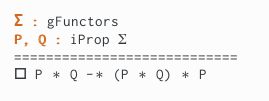
\includegraphics[scale=0.7]{sections/graphics/proofmode-0.png}
\end{center}
Ignoring $\Sigma$, which has to do with specifying which resource algebras are available, this is an ordinary Coq goal.
The assumptions are that $P$ and $Q$ are Iris propositions, and the goal is to prove the entailment.
Note that the $\vdash$ is replaced with $-\ast$, for reasons which are not important.
It is simply different notation for the same thing.

We then enter the proof mode at which point our goal looks as follows.
\begin{center}
  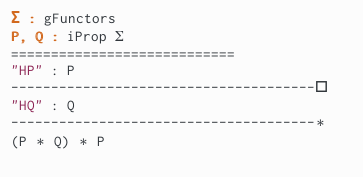
\includegraphics[scale=0.7]{sections/graphics/proofmode-1.png}
\end{center}
The Coq context, above the double line, stays the same, but the goal is different.
It consists of two contexts, and a conclusion.
The first context contains one assumption $P$, named \texttt{HP}.
Assumptions are named so that they can be referred to by tactics, analogously how assumptions are named in ordinary Coq proofs, except that for engineering reasons names of Iris assumptions need to be quoted as strings.
This is the context of \emph{persistent assumptions}.
Every assumption in this context implicitly has an $\persistently$ modality around it.

The second context also contains one assumption, $Q$, and the assumption has name \texttt{HQ}.
This is a context of arbitrary Iris assertions.

To prove the goal, if we were using the rules of the logic directly, we would duplicate the assumption $\persistently P$, and then use the separating conjunction introduction rule.
There is a tactic which corresponds to the separating conjunction introduction rule,\footnote{There are in fact two, \texttt{isSplitL}, and \texttt{iSplitR}.} and the tactic knows that persistent assertions can be duplicated.
Thus using this tactic we get the following two goals.
\begin{center}
  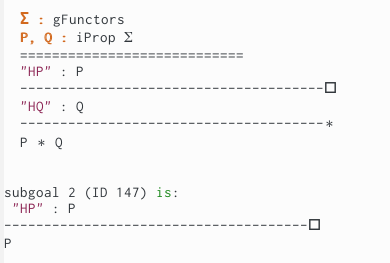
\includegraphics[scale=0.7]{sections/graphics/proofmode-2.png}
\end{center}
Notice how in the first goal we have assertions $P$ and $Q$ available, whereas in the second we only have $P$ available, since $Q$ is not persistent.

In the accompanying Coq example files we explain how to use the tactics and manipulate contexts to achieve this.

\paragraph*{Hoare triples in Iris Coq}
One point of difference of the Iris logic in Coq as opposed to the one presented in this paper is the definition of Hoare triples.
Recall that we defined Hoare triples as
\begin{align*}
  \hoare{P}{e}{\Phi} \eqdef \persistently\left(P \wand \wpre{e}{\Phi}\right).
\end{align*}
In Coq they are defined slightly differently, using the similar mode of use of weakest precondition specifications with an arbitrary postcondition.
To wit, they are defined as
\begin{align*}
  \hoare{P}{e}{\Phi}[\mask] \eqdef \persistently\left(\forall \Psi, P \wand \later(\forall v, \Phi(v) \wand \Psi(v)) \wand \wpre{e}[\mask]{\Psi}\right).
\end{align*}
If there was no later modality the two definitions would be rather trivially equivalent.
The reason for introducing the later modality is technical, and it is there purely for reasons of convenience.
\begin{exercise}
  Show that for expressions $e$ \emph{which are not values} the two definitions are logically equivalent.
\end{exercise}

Thus, the only place where they differ slightly is for values.
But since these triples are in practice never used for values, they are only used for top-level specifications, it does not matter.

%%% Local Variables:
%%% mode: latex
%%% TeX-master: "../main.tex"
%%% End:



\section{On Inductive, Coinductive, and Guarded-Recursive Predicates}
\label{sec:inductive-coinductive-predicates}


In standard higher-order logic one can define inductive and coinductive predicates
via so-called \emph{higher-order definitions}. In this section, we show how this can also be done
in Iris, and we discuss the relationship between inductive, coinductive, and guarded-recursive predicates.

This whole section can be skipped; indeed, we only include this section ``for general interest'' and to prepare the reader for more advanced
applications (\eg\ inductive predicates can be used to \emph{define} a notion of total weakest precondition,
useful for reasoning about \emph{total} correctness instead of the \emph{partial} correctness we consider
in these lecture notes and which is definable using guarded recursion \cite{iris-ground-up}).

For the remainder of this section we fix an Iris type $\tau$ and we will consider how to define predicates
on $\tau$, \ie\ functions of type $\tau\to\Prop$. We first give a somewhat informal preview and then
present a more systematic formal account; for brevity we omit most proofs and leave them for the reader
as interesting exercises.\footnote{Formal proofs in Iris in Coq can be found in the accompanying coq file \texttt{fixpoint.v}.}

\paragraph{Preview} 
We have already seen two ways of defining predicates on $\tau$, which we now call to mind.
First, recall the $\operatorname{isList}$ predicate defined in Section \ref{sec:basic-separation-logic}.
There we explained that $\operatorname{isList} l\, xs$ relates a programming language value $l$ to a mathematical sequence of values
$xs$, \ie\ $\operatorname{isList}$ is of type $\Val\to\operatorname{Seq}(\Val)\to\Prop$,
and that it was defined by induction on the mathematical sequence $xs$.  Observe: $\operatorname{Seq}(\Val)$ is
an Iris \emph{type} of standard mathematical sequences and we use that to define a new predicate $\operatorname{isList}$.
Now, what if we do not care about which mathematical sequence $l$ represents, but just want to express
that $l$ is a linked list representing some unknown sequence of elements ?
Then we can, of course, define a new predicate
$\operatorname{MList} : \Val\to\Prop$ by setting $\operatorname{MList} l = \Exists xs. \operatorname{isList} l\, xs$.
But we could also define a predicate by guarded recursion by letting
\begin{displaymath}
  \operatorname{GList} = \MU \phi:\Val\to\Prop. \lambda l .
    l = \langkw{inj}_1() \lor  \Exists hd, x, l'. l = \langkw{inj}_2(hd) * hd \pointsto (x,l') * \later \phi(l').
\end{displaymath}
Note that $\operatorname{GList}$ is well-defined since $\phi$ (only) occurs under a later $\later$ modality.
Intuitively, $\operatorname{GList}(l)$ holds if either $l$ is the empty list or if $l$ points to a
pair with a head and tail element such that $\operatorname{Glist}$ holds for the tail element \emph{later}.

Since all of our linked-list operations in Section \ref{sec:basic-separation-logic} always take a step
to access the tail of a linked list, this definition would also allow us to prove safety of
the linked list operations.
\begin{exercise}
  Use $\operatorname{GList}$ to prove the following Hoare triple that expresses that the
  increment function from Section \ref{sec:basic-separation-logic} is safe:
    \begin{mathpar}
    \forall l.
    \hoare{\operatorname{GList} l}{\langkw{inc}\, l}{v. v = () \wedge \operatorname{GList} l}
  \end{mathpar}
  Use L\"ob induction and take care to note how we get to remove the later modality we get
  from the definition of $\operatorname{GList}$.
\end{exercise}

Now take a closer look at the definition of $\operatorname{GList}$ and rewrite it as follows.
First, define function $F: (Val\to\Prop)\to(\Val\to\Prop)$ by
\begin{displaymath}
  F(\phi) =
  l = \langkw{inj}_1() \lor  \Exists hd, x, l'. l = \langkw{inj}_2(hd) * hd \pointsto (x,l') * \phi(l').
\end{displaymath}
Then $\operatorname{GList} = \MU \phi. F(\later \phi)$.
But since $\phi$ only occurs \emph{positively} 
in $F(\phi)$, the function $F: (Val\to\Prop)\to(\Val\to\Prop)$ is in fact a \emph{monotone} function and
hence it has a least and a greatest fixed point --- we will define what monotonicity means and
prove that such least and greatest fixed points do indeed exist below.
The least fixed point of $F$ is an inductive predicate; indeed, \emph{by an inductive predicate we mean
a predicate defined as the least fixed point of a monotone function}. 
Likewise, the greatest fixed point of $F$ is a coinductive predicate; and, indeed, \emph{by an coinductive predicate we mean
  a predicate defined as the greatest fixed point of a monotone function}.

Thus we could also have defined a predicate $\operatorname{IList}$ as the least fixed point of $F$
and a predicate $CoIList$ as the greatest fixed point of $F$. Then we would have
three candidate formal definitions of predicates corresponding to the intuitive linked list predicate.
In this particular case, all three predicates, the inductive
$\operatorname{IList}$ and the coinductive $\operatorname{CoIList}$ predicates coincide
(in the sense that $\operatorname{IList} \provesIff \operatorname{CoIList}$) and
is closely related to the guarded-recursive $\operatorname{GList}$ predicate
(in the sense that $\operatorname{CoIList} \proves \operatorname{GList}$ and
if $\TRUE\proves\operatorname{GList}$ then $\TRUE\proves\operatorname{CoIList}$).
This is not entirely trivial to see, but can be proved using the model of Iris;
it rests on the fact that the programming language values and the heap are finite, and
that the definition of $F$ does not allow for cycles in the heap because of the use of $*$.
However, in general, inductive, coinductive and guarded recursive predicates (obtained from the
same monotone operator) are not the same; we will present an example that illustrates the
differences in the following. We will do so by working entirely in the Iris \emph{logic}, \ie\ without
having to understand the semantics of Iris.
Before we begin on the more formal treatment, however, we hasten to point out one key difference between guarded-recursive
predicates and inductive / coinductive predicates: to define a guarded-recursive predicate, we do not
need to require that the induced function $F$ is monotone; as long as the recursion variable (the variable $\phi$ above)
occurs under a later $\later$ modality, then the predicate is well-defined.
We make use of this flexibility in Section \ref{sec:logical-relations} to define a logical relations interpretation
of recursive types. (For a program verification example that relies on this flexibility, see
the event loop example in the iCap logic \cite{icap} -- iCap is a precursor to Iris.)

\paragraph{Background on fixed point theorems on complete lattices}

To understand the higher-order definitions below, it is useful to recall Tarski's fixed point theorem on complete lattices.
(for a thorough introductory account, see \cite{davey-priestley-2002}):
Suppose $L$ is a complete lattice and that $f$ is a monotone function on $L$.
Then $f$ has a least fixed point given by $\bigcap \{ \phi \,\mid\, f \phi \leq \phi \}$,
the intersection of all prefixed points,
and a greatest fixed point given by $\bigcup \{ \phi \,\mid\, \phi \leq f\phi \}$, the union
of all postfixed points.
Consider the special case where $L$ is the powerset of some given set $X$, \ie\ $L = X\to\Prop$,
and the ordering $\leq$ is the subset ordering. In this case the least fixed point, e.g., is given by
$\bigcap \{ \phi \,\mid\, \forall x.\, f \phi x \implies \phi x \}$.
In higher-order logic, one can prove that the higher-order logic rendition of this formula, \ie\
$\forall \phi.\, (\forall x.\, f \phi x \implies \phi x) \implies \phi$ is a fixed point of
$f: (X\to\Prop)\to(X\to\Prop)$ when $f$ is monotone.
Similarly, one can obtain a higher-order logic definition of the greatest fixed point based on Tarski's
greatest fixed point formula.
In our situation, with our Iris resource logic, 
we will use the persistence modality to
ensure that the notions of monotonicity, prefixed point, and postfixed point do not
depend on any resources. 


\paragraph{A More Systematic Account}


Let $\tau$ be an Iris type and let $F:(\tau\to\Prop)\to(\tau\to\Prop)$ be an endofunction on the type of predicates on $\tau$.

\begin{definition}
  We say that $F$ is \emph{monotone} if, for all $\phi,\psi: \tau\to\Prop$, it holds that
  \begin{displaymath}
    \persistently(\forall x. \phi x \wand \psi x) \implies
    \forall x. F \phi x \wand F \psi x.
  \end{displaymath}
\end{definition}


\newcommand{\lfp}{\operatorname{lfp}}
\newcommand{\gfp}{\operatorname{gfp}}
\newcommand{\grd}{\operatorname{grd}}

\begin{definition}
  Suppose  $F:(\tau\to\Prop)\to(\tau\to\Prop)$ is monotone. We then define
  $\lfp F: \tau\to\Prop$, $\gfp F : \tau\to\Prop$, and $\grd F: \tau\to\Prop$ by
  \begin{align*}
    \lfp F & = \lambda x:\tau. \forall \phi:\tau\to\Prop.
             \persistently (\forall x. F \phi x \wand \phi x) \implies \phi x\\
    \gfp F & = \lambda x:\tau. \exists \phi:\tau\to\Prop.
             \persistently (\forall x. \phi x \wand F \phi x) \land \phi x \\
    \grd F & = \MU \phi:\tau\to\Prop. F(\later \phi).
  \end{align*}
\end{definition}

As the names suggest, $\lfp F$ is the least fixed point of $F$, $\gfp F$ is the greatest
fixed point of $F$, and $\grd F$ is the guarded recursive predicate defined by $F$.
The latter is by definition, whereas the least and greatest fixed point properties require proof. 
We now state the claims precisely using a series of lemmas, which
are instructive to prove. We leave the proofs as exercises to the reader.
As mentioned above, by \emph{the inductive predicate defined by $F$} we mean $\lfp F$, and
by \emph{the coinductive predicate defined by $F$} we mean $\gfp F$.
  
\begin{lemma}[$\lfp F$ is a fixed point of $F$, up to provability]
  \begin{align*}
    \forall x.\, F (\lfp F) x  \provesIff  \lfp F x
  \end{align*}
\end{lemma}

\begin{lemma}[Induction Principle]
  For all $\phi: \tau\to\Prop$,
  \begin{align*}
    \persistently(\forall y.\, F \phi y \wand \phi y) \wand
    \forall x.\, \lfp F x \wand \phi x.
  \end{align*}
\end{lemma}

\begin{lemma}[Strong Induction Principle]
  For all $\phi: \tau\to\Prop$,
  \begin{align*}
    \persistently(\forall y.\, F (\lambda x. \phi x \land \lfp F x) y \wand \phi y) \wand 
    \forall x.\, \lfp F x \wand \phi x.
  \end{align*}
\end{lemma}

\begin{lemma}[$\gfp F$ is a fixed point of $F$, up to provability]
  \begin{align*}
    \forall x.\, F (\gfp F) x  \provesIff  \gfp F x.
  \end{align*}
\end{lemma}

\begin{lemma}[Coinduction Principle]
  For all $\phi: \tau\to\Prop$,
  \begin{align*}
    \persistently(\forall y.\, \phi y \wand F \phi y) \wand
    \forall x.\, \phi x \wand \gfp F x.
  \end{align*}
\end{lemma}


To get a better intuitive understanding of inductive, coinductive, and guarded recursive predicates,
and how they relate, 
we consider an example, namely reachability in the following infinite graph $G$.

\begin{center}
  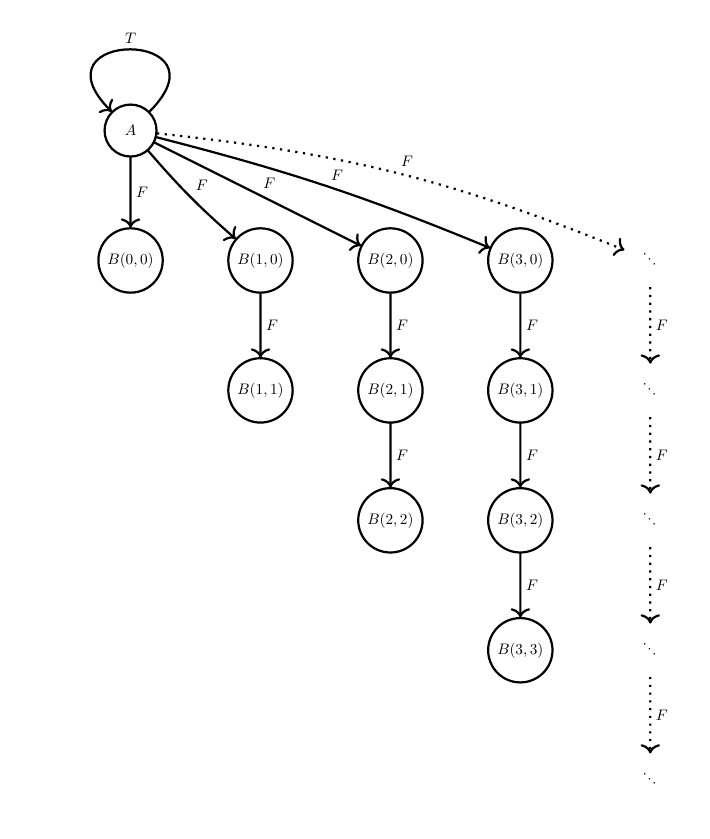
\begin{tikzpicture}[term/.style={circle,draw,minimum size=12mm,inner sep=4pt},auto , scale=0.55, every node/.style={scale=0.55}]
    \node [thick] (A) at (0,0) [term] {$A$};
    \node [thick] (B00) at (0,-3) [term] {$B(0,0)$};
      \node [thick] (B10) at (3,-3) [term] {$B(1,0)$}; \node [thick] (B20) at (6,-3) [term] {$B(2,0)$}; \node [thick] (B30) at (9,-3) [term] {$B(3,0)$}; \node[inner sep=10, rotate=-45] (B40) at (12,-3) {$\cdots$};
    \node [thick] (B11) at (3,-6) [term] {$B(1,1)$}; \node [thick] (B21) at (6,-6) [term] {$B(2,1)$}; \node [thick] (B31) at (9,-6) [term] {$B(3,1)$}; \node[inner sep=10, rotate=-45] (B41) at (12,-6) {$\cdots$};
    \node [thick] (B22) at (6,-9) [term] {$B(2,2)$}; \node [thick] (B32) at (9,-9) [term] {$B(3,2)$};
\node[inner sep=10, rotate=-45] (B42) at (12,-9) {$\cdots$};
    \node [thick] (B33) at (9,-12) [term] {$B(3,3)$};
    \node[inner sep=10, rotate=-45] (B43) at (12,-12) {$\cdots$};
    \node[inner sep=10, rotate=-45] (B44) at (12,-15) {$\cdots$};
%    
    \draw [->,thick,loop] (A) to node[above] {$T$} (A);
    \draw [->,thick] (A) to node {$F$} (B00);
    \draw [->,thick, bend right=4] (A) to node {$F$} (B10);
    \draw [->,thick] (A) to node {$F$} (B20);
    \draw [->,thick, bend left=4] (A) to node {$F$} (B30);
    \draw [->,thick, dotted, bend left=8] (A) to node {$F$} (B40);
%    
    \draw [->,thick] (B10) to node {$F$} (B11);
%
    \draw [->,thick] (B20) to node {$F$} (B21); \draw [->,thick] (B21) to node {$F$} (B22);
%   
    \draw [->,thick] (B30) to node {$F$} (B31); \draw [->,thick] (B31) to node {$F$} (B32); \draw [->,thick] (B32) to node {$F$} (B33);
%
    \draw [->,thick, dotted] (B40) to node {$F$} (B41); \draw [->,thick, dotted] (B41) to node {$F$} (B42); \draw [->,thick, dotted] (B42) to node {$F$} (B43); \draw [->,thick, dotted] (B43) to node {$F$} (B44);
  \end{tikzpicture}
\end{center}

\newcommand{\StrB}{\operatorname{Stream}(B)}
\newcommand{\NodeG}{\operatorname{Node}}

The graph $G$ is an element of a \emph{type} of graphs with nodes $A$ or $B(n,m)$ (with $m\leq n$) and with
edges labelled with a boolean $T$ or $F$. We assume that this type of graphs is available in Iris, just like we assumed that
the type of finite mathematical sequences is, see Section~\ref{sec:basic-separation-logic}. We also assume that
the type of nodes is available and denote it by $\NodeG$.
Moreover, we assume that we have an Iris type of mathematial streams (finite or infinite sequences) available; we write
$\operatorname{Stream}(B)$ for the type of streams of booleans $B=\{T,F\}$, and we write $[]$ for the empty stream,
and $l::ls$ for the stream with head $l$ and tail $ls$.

We will now consider different ways of defining reachability in the graph $G$.
Specifically, we will define predicates that express that, starting from some specific node,
a stream of booleans is reachable in $G$.
(For example, looking at the picture of $G$ above, since there is a loop from node $A$ to $A$
labelled $T$, it is intuitively clear that the constant infinite stream of $T$'s is reachable from $A$.)
Thus we will be interested in predicates on the type $\tau=\NodeG\times \StrB$.

Consider now the following function $F: (\NodeG\times \StrB\to\Prop) \to (\NodeG\times \StrB\to\Prop)$:
\begin{align*}
  F \psi = \lambda (x, ls).\,
    ls = [] \lor
    \exists y, l, ls'.\, ls = l::ls' \land \operatorname{Edge}(G,x,y,l) \land \psi y ls'
\end{align*}
where $\operatorname{Edge}(G,x,y,l)$ means that there is an edge from node $x$ to node $y$ in the graph $G$ with label $l$.

\begin{lemma}
  $F$ is monotone.
\end{lemma}

Since $F$ is monotone, the least and greatest fixed points $\lfp F$ and $\gfp F$ of $F$ exist,
as does the guarded recursive predicate $\grd F$. Each of these define a notion of reachability.


\begin{lemma}
  \label{lem:lfp-gfp-grd}
  \begin{align*}
    \forall x:\tau.\,
    \lfp F x \proves \gfp F x \proves \grd F x.
  \end{align*}
\end{lemma}

The following lemmas express that the inductive notion of reachability
only contains finite paths. 

\begin{lemma}
  \label{lem:lfp-finite}
  Let $ls$ be a \emph{finite} sequence of constant $T$'s or constant $F$'s.
  Then $\lfp F (A,ls)$ holds.
\end{lemma}

\begin{lemma}
  \label{lem:lfp-infinite}
  Let $ls$ be an \emph{infinite} sequence of constant $T$'s or constant $F$'s and let $n$ be any node.
  Then $\lfp F (n,ls)$ does not hold, (i.e., $\lfp F (n,ls) \proves \FALSE$).
\end{lemma}

The following lemmas express that the coinductive notion of reachability
not only includes finite paths, but also infinite paths.


\begin{lemma}
  Let $ls$ be the \emph{infinite} sequence of constant $T$'s.
  Then $\gfp F (A,ls)$ holds.
\end{lemma}

\begin{lemma}
  Let $ls$ be the \emph{infinite} sequence of constant $F$'s and let $n$ be any $B$ node.
  Then $\gfp F (n,ls)$ does not hold (i.e., $\gfp F (n,ls) \proves \FALSE$).
\end{lemma}

\begin{lemma}
  Let $ls$ be the \emph{infinite} sequence of constant $F$'s and let $n$ be any node.
  Then $\gfp F (n,ls)$ does not hold (i.e., $\gfp F (n,ls) \proves \FALSE$).
\end{lemma}

Intuitively, the following lemma captures that guarded-recursive predicates are ``closed under limits'':
by Lemmas \ref{lem:lfp-gfp-grd} and \ref{lem:lfp-finite} every finite path of constant $F$'s is in the guarded-recursive notion of reachability;
this is used to prove the following lemma, which says that also the limit, the \emph{infinite} sequence of constant $F$'s, is in the guarded-recursive notion of reachability.

\begin{lemma}
  Let $ls$ be the \emph{infinite} sequence of constant $F$'s.
  Then $\grd F (A,ls)$ holds.
\end{lemma}

We finally remark that guarded-recursive predicates are in fact unique (we did not include a proof rule expressing that in Section \ref{sec:recursively-defined-pred}) and that is exactly because their behaviour at limit points is determined by what happens at finite approximants.


%%% Local Variables:
%%% mode: latex
%%% TeX-master: "../main.tex"
%%% End:



\section{The later modality and steps of computation}
\label{sec:later-steps}

When explaining the later modality and weakest preconditions we explained informally that
the later modality is tied to physical steps of computation (\ie{} steps in the small-step operational semantics of the programming language).
Formally, this can be seen in the actual definition of weakest preconditions, which we do not present in these notes but which can be seen in \cite{iris-ground-up}.
That being said, it is very instructive to look at this relationship within the logic, \ie{} using just what we have seen so far.
To shed some light on this relationship, in this section we look at an example of a program that is only safe, \ie{} does not get stuck, for a few steps of computation, and see what we can show in \Iris{} about such a program.
First, however, we take a closer look at how we can formally state in \Iris{} that a statement holds for a certain number of steps.

In the formal language of \Iris{} we formalize a proposition holding for a number of steps as follows:
\begin{definition} Given a proposition $\prop$ we say that $\prop$ holds for $k$ steps if and only if the following holds:
\begin{align*}
  {\later}^{k} \FALSE \proves \prop \tag{$\prop$ holds for $k$ steps}
\end{align*}
\end{definition}
This makes intuitive sense: if $\prop$ holds under the assumption that $\FALSE$ holds after $k$ steps, then $\prop$ must hold for $k$ steps.
In addition, we have that for a proposition $\prop$,
\begin{align}
\proves \prop \text{ holds if and only if for \emph{any} } k \text{ we have } {\later}^{k} \FALSE \proves \prop \text{ holds} \label{eq:holds-if-for-all-steps}
\end{align}
This again makes intuitive sense: $\prop$ holds if and only if it holds for arbitrarily many steps.
The \emph{only if} direction of the above statement \eqref{eq:holds-if-for-all-steps} is trivial.
The \emph{if} direction, on the other hand, is not.
It follows, rather easily (left as an exercise), from the following:
\begin{align}
  \proves \exists k.\; {\later}^{k} \FALSE \label{eq:expose-steps}
\end{align}
The statement \eqref{eq:expose-steps} above, which might be a bit surprising at first sight, is in fact logically equivalent to \ruleref{Loeb} induction.
Before showing this however, let us ponder the intuitive meaning of \eqref{eq:expose-steps}.
It says that there is exists a number $k$ such that $\FALSE$ holds after $k$ many steps.
Recall that \Iris{} is a step-indexed logic where the intuitive meaning of $\proves \prop$ is that for any $j$, $\prop$ holds for $j$ steps.
With this intuition in mind, \eqref{eq:expose-steps} essentially says that for any $j$ the following holds for $j$ steps: there exists a number $k$ such that after $k$ steps $\FALSE$ holds.
Since we are considering the truth of the statement ``there exists a number $k$ \dots'' only up to $j$ steps, we can simply take $k$ to be any number greater than $j$.
Then, by definition, we don't care about what happens after $k$ steps because it is already beyond the $j$ many steps that we care about.
The crucial point here is the interpretation of the existential quantifier in our step-indexed logic.
It allows us to pick different $k$'s for the different number of steps being considered.
A deep and thorough consideration of the intuitive meaning behind the proof of the following theorem should reveal the intuitive reasoning we just discussed for why \eqref{eq:expose-steps} holds.

\begin{remark}
  Note that the statement \eqref{eq:expose-steps} holding, \ie{} $\proves \exists k.\; {\later}^{k} \FALSE$, does not imply that there is in fact some number $n$ for which $\proves {\later}^{n} \FALSE$ holds.
  The key point here is that the existential quantifier can be instantiated to be a different natural number depending on the current step-index.
  The proposition $\proves {\later}^{n} \FALSE$ cannot hold (\ie{} cannot hold for all step-indices) for any fixed $n$ because for any fixed $n$ it would not hold for step-indices greater than $n$.
\end{remark}

\begin{theorem}
  Statement \eqref{eq:expose-steps} is equivalent to the principle of \ruleref{Loeb} induction.
\end{theorem}

\begin{proof}
{\bfseries [\eqref{eq:expose-steps} \emph{is implied by} \ruleref{Loeb}]}
We need to show $\proves \exists k.\; {\later}^{k} \FALSE$.
By \ruleref{Loeb} induction it suffices to show that $\later \exists k.\; {\later}^{k} \FALSE \proves \exists k.\; {\later}^{k} \FALSE$.
Now, we can use the \ruleref{later-exists} rule.
Hence, we have to show that $\exists k.\; {\later}^{k+1} \FALSE \proves \exists k.\; {\later}^{k} \FALSE$.
We then eliminate the existential quantifier as the natural number $l$ which leaves us to show ${\later}^{l+1} \FALSE \proves \exists k.\; {\later}^{k} \FALSE$.
We simply take $k$ to be $l + 1$, or any number larger than that, to finish the proof.\\

\noindent
{\bfseries [\eqref{eq:expose-steps} \emph{implies} \ruleref{Loeb}]}
We need to show that $\propB \proves \prop$ given that $\propB \land \later \prop \proves \prop$.
Now, by \eqref{eq:expose-steps} we can add $\exists k.\; {\later}^{k} \FALSE$ to our hypotheses, since we are assuming it holds.
Thus it suffices to show that $\propB \land \exists k.\; {\later}^{k} \FALSE \proves \prop$.
We proceed by eliminating the existential quantifier as the natural number $l$ which leaves us to show $\propB \land {\later}^{l} \FALSE \proves \prop$.
We proceed by induction on $l$.
The base case is trivial: we have to show that $\propB \land \FALSE \proves \prop$.
For the inductive case, we can assume (induction hypothesis) that $\propB \land {\later}^{l} \FALSE \proves \prop$ and have to show $\propB \land {\later}^{l+1} \FALSE \proves \prop$.
Now, by our starting hypothesis, (the antecedent of \ruleref{Loeb}) we have that $\propB \land \later \prop \proves \prop$.
Hence, it suffices to show that $\propB \land {\later}^{l+1} \FALSE \proves \propB \land \later \prop$ to conclude the proof.
Obviously, $\propB \land {\later}^{l+1} \FALSE \proves \propB$ holds.
Therefore, we only need to show $\propB \land {\later}^{l+1} \FALSE \proves \later \prop$.
We proceed by weakening $\propB$ by putting it under a later modality.
That is, we need to show $\later \propB \land {\later}^{l+1} \FALSE \proves \later \prop$.
And since later commutes with conjunction (\ruleref{Later-conj}) we simply need to show $\later (\propB \land {\later}^{l} \FALSE) \proves \later \prop$.
Finally, the \ruleref{Later-Mono} rule can be applied which leaves us to show $\propB \land {\later}^{l} \FALSE \proves \prop$.
This is precisely our induction hypothesis (the induction we performed on $l$) which concludes the proof.
\end{proof}

To summarize, what we have seen so far captures, in the formal language of the logic, what we intuitively think when we think about step-indexing in \Iris{}.
The proposition ${\later}^{k} \FALSE$ holds if we are proving things only up to $k$ steps.
When we are proving a proposition $\prop$ in \Iris{} we are essentially showing that for any $k$ the proposition $\prop$ holds for $k$ steps \eqref{eq:holds-if-for-all-steps}.
And that there is always a step-index $k$ such that we are proving things only up to $k$ steps \eqref{eq:expose-steps}.
Note how the latter intuition essentially tells us that the reason why \ruleref{Loeb} induction holds is that we can perform induction on the step-index; this, \ie{} induction on the step-index, is exactly how one proves the principle of \ruleref{Loeb} induction sound in the model of \Iris{} \cite{iris-ground-up}.

Now, let us consider the following program which is \emph{not} safe.
It crashes, \ie{} gets stuck, but only after two steps of computation.
\[ \langkw{let}~ \mathit{twoSteps} = (\lambda \var. \If \var then 2 \Else 3 + \var)~\False \]
Since \Iris{} ties physical steps of computation (in the sense of small-step operational semantics) to logical steps, \ie{} the later modality, we should be able to show the following:
\begin{align*}
  \proves \hoare{{\later}^{2} \FALSE}{\mathit{twoSteps}}{\var.\; \FALSE}
\end{align*}
And we can.
After applying the rule \ruleref{Ht-beta} corresponding to the function application step we need to show
\begin{align*}
  \proves \hoare{\later \FALSE}{\If \False then 2 \Else 3 + \False}{\var.\; \FALSE}
\end{align*}
Now we can use the rule \ruleref{Ht-If} for conditionals which leaves us to show
\begin{align*}
  \proves \hoare{\FALSE \ast \False = \True}{3 + \False}{\var.\; \FALSE}
\end{align*}
and
\begin{align*}
  \proves \hoare{\FALSE \ast \False = \False}{3 + \False}{\var.\; \FALSE}
\end{align*}
Both of which hold vacuously.
Note how in this proof the postcondition is irrelevant as the program never terminates within the two steps of computation that we are considering it.

%%% Local Variables:
%%% mode: latex
%%% TeX-master: "../main.tex"
%%% End:


\section{Case Study: Types and Abstraction: Logical Relations in Iris}
\label{sec:logical-relations}

This section is still work-in-progress. It is closely based on~\cite{timany:logrel-in-iris};
indeed large parts of this section are taken directly from~\cite{timany:logrel-in-iris},
with permission from the authors.

\newcommand{\EqTyp}{\mathsf{EqType}}
\newcommand{\TheLang}{\(\mathsf{F}_{\mu, \mathit{ref}, \mathit{conc}}\)}
\newcommand{\SAFE}{\mathit{Safe}}
\newcommand{\lectx}{\le_{\mathit{ctx}}}
\newcommand{\lelog}{\le_{\mathit{log}}}
\newcommand{\valC}{u}
\newcommand{\len}{\mathrm{length}}

%%%%%%%%%%%%%%%%%%%%%%%%%%%%%%%%%%%%%%%%%%%%%%%%%%%%%%%%%%%%%%%%
% Logical relations
%%%%%%%%%%%%%%%%%%%%%%%%%%%%%%%%%%%%%%%%%%%%%%%%%%%%%%%%%%%%%%%%

\newcommand{\semVtype}[3]{ \llbracket #1 \vdash #2 \rrbracket_{#3} }
\newcommand{\semEtype}[3]{ \llbracket #1 \vdash #2 \rrbracket^{\mathcal{E}}_{#3} }
\newcommand{\semGtype}[3]{ \llbracket #1 \vdash #2 \rrbracket^{\mathcal{G}}_{#3} }

\newcommand{\cfgg}{\rho}
\newcommand{\SpecConf}{\textrm{SpecConf}}
\newcommand{\SpecCtx}{\textrm{SpecCtx}}

\renewcommand{\qedsymbol}{$\square$}

So far we have used Iris for specifying and reasoning about programs written in the
\emph{untyped} programming language \proglang. 
In this section we will consider a \emph{typed} programming language,
\TheLang,  and show how we can use Iris to give semantic interpretations
of the types of \TheLang.  

In the words of Reynolds~\cite{reynolds:types}, a type system ``is a syntactic
discipline for enforcing levels of abstraction''.
One of the fundamental properties of a type system is type
soundness, \ie\ that ``syntactically well-typed programs don't go wrong''~\cite{Milner:78}.
In contrast to the properties we have considered earlier in these
notes, where we so far have focused on properties of individual
programs, type soundness is a language property: it is a property that 
depends on the operational semantics and the type system for the whole
programming language and it is a property that one proves once and 
for all for a programming language. 
There are different approaches to proving type soundness, most notably
the syntactic approach based on progress and preservation lemmas (for
textbook treatments, see, e.g.,~\cite{pierce:tapl,harper:practical-foundations}), and 
the semantic approach where one gives a semantic model of the types 
and proves that any syntactically well-typed program is in the
semantic interpretation of its type. 

An advantage of the semantic approach is that it gives a semantic account of the invariants
enforced by the syntactic type system. This means that it allows one
to \emph{combine} syntactically well-typed programs with programs which are
semantically, but not necessarily syntactially, well-typed. This is
important in practise since most realistic statically typed programming
languages include some facility for interacting with programs that are
not syntactically well typed (e.g., through foreign function call
interfaces, or through an ``unsafe'' construct~\cite{}). 

An advantage of the syntactic approach using progress and preservation
lemmas is that it scales well to advanced type systems including
impredicative polymorphism, recursive types, and general reference
types. In contrast, an often-cited challenge with the semantic
approach is that it is non-trivial to define semantic interpretations of advanced type
systems (because the semantic models need to support recursive
definitions and impredicative invariants). 

In this section we show that \emph{by interpreting types as 
Iris propositions it is straightforward to give a semantic
interpretation of types}, and prove that all syntactically well-typed
programs are in the appropriate semantic interpretation. Moreover,
we can also use Iris to show semantic well-typedness of 
programs that are not syntactically well-typed.

The key point is that we can exploit Iris features such as invariants, persistence, and the possibility of defining predicates by guarded recursion to give a simple inductive definition of the interpretation of all the types of \TheLang, which include challenging types such as impredicative polymorpic types, recursive types, and general reference types.
We focus on type soundness in Subsection~\ref{sec:unary-logical-relation}.

Another advantage of the semantic approach is that it can be
generalized to give a \emph{relational interpretation} of types, which
is useful for proving contextual refinement and data abstraction results.
It is well-known that relational models for showing contextual refinement are also
non-trivial to construct. Moreover, it is particularly challenging to
construct relational models which are sufficiently powerful to allow
one to prove relatedness of programs that use state and concurrency in
very different ways. Using Iris, however, we can addresss both of
these challenges. Indeed, in~\cite{timany:logrel-in-iris} a relational
interpretation of the types of \TheLang\ is also defined, by
interpreting types as Iris relations. Moreover, it is shown that the
relational interpretation is expressive enough to allow one to prove
challenging examples of program refinements. For example, it is proved
that a fine-grained concurrent stack module is a contextual refinement of a
coarse-grained stack module. 
In light of the fact that we so far only used Iris for reasoning about a
single program at a time, it is perhaps somewhat surprising that we can also
use Iris to relate two different programs.  Thus, in
Subsection~\ref{sec:binary-logical-relation} we sketch the key idea of
how this can be done. 
However, we do not include a full description of the relational
model, but instead refer the reader to~\cite{timany:logrel-in-iris}. 


\subsection{The language \texorpdfstring{\TheLang}{Fmurefconc}}
\TheLang\, is mostly as \proglang, the main exception being that it is a typed languages. We have all the same values and expressions as before with a few additions: 
\begin{itemize}
\item \langkw{fold} and \langkw{unfold} respectively fold and unfold expressions of recursive types.
\item $\Lambda$ is a type-level lambda abstraction.
\end{itemize}
\begin{figure}[htbp]
\textbf{Syntax}
\begin{displaymath}
  \begin{array}{lrcl}
\Val\quad
& \val & \bnfdef{}&
 \cdots
 \ALT \langkw{fold}\, \val
 \ALT \Lambda \, \expr
\\
%
\Expr \quad
& \expr & \bnfdef{} &
 \cdots
 \ALT \langkw{fold} \, \expr
 \ALT \langkw{unfold} \, \expr
 \ALT \Lambda \, \expr 
 \ALT \expr \, \_
\\
%
\ECtx\quad
& E & \bnfdef{}& 
 \cdots
 \ALT \langkw{fold} \, E
 \ALT \langkw{unfold} \, E
 \ALT E \, \_ 
 \\
%
 Types \quad & \typ & \bnfdef{}& 
 X
 \ALT 1
 \ALT \nat
 \ALT \mathbb{B}
 \ALT \typ \to \typ
 \ALT \All X. \typ
 \ALT \typ \times \typ
 \ALT \typ + \typ
 \ALT \mu X. \typ
 \ALT ref \typ
\\
%
\end{array}
\end{displaymath}
\end{figure}
We have the same reductions as \proglang{} with the addition of the following two pure reductions:

\begin{align*}
 \left( \Lambda \, \expr \right)\, \_ &\stepstopure \expr \\
 \langkw{unfold}\, (\langkw{fold}\, \val) &\stepstopure \val
\end{align*}


As the weakest precondition is defined from the operational semantics, we get the same wp-rules as in Figure~\ref{fig:wp-rules} with the addition of the following two rules, corresponding to our two new reductions:

\begin{mathpar}
\inferH{wp-Tlam}{}{\later \wpre{\expr}[\mask]{\pred}\proves \wpre{(\TLam \expr)~\_}[\mask]{\pred}}
\and
\inferH{wp-fold}{}{\later \wpre{\val}[\mask]{\pred}\proves \wpre{\unfold(\fold \val)}[\mask]{\pred}}
\end{mathpar}

To make \TheLang\, a typed language, we naturally need some typing rules. These are fairly standard (see~\cite{pierce:tapl,harper:practical-foundations})
and given in Figure~\ref {fig:logrel-iris-typing-rules}.


\begin{figure}
\begin{mathparpagebreakable}
  \inferH{T-var}{\var : \typ \in \env}{\typed{\Tenv}{\env}{\var}{\typ}}
  \and
  \inferH{T-Unit}{}{\typed{\Tenv}{\env}{\TT}{\Tunit}}
  \and
  \inferH{T-Nat}{}{\typed{\Tenv}{\env}{n}{\Tnat}}
  \and
  \inferH{T-Bool}{\val \in \set{\True, \False}}{\typed{\Tenv}{\env}{\val}{\Tbool}}
  \and
  \inferH{T-rec}{\typed{\Tenv}{\env, \var : \typ, f : \typ \to \typ'}{\expr}{\typ'}}
  {\typed{\Tenv}{\env}{\Rec f \var = \expr}{\typ \to \typ'}}
  \and
  \inferH{T-app}{\typed{\Tenv}{\env}{\expr_1}{\typ \to \typ'} \and \typed{\Tenv}{\env}{\expr_2}{\typ}}
  {\typed{\Tenv}{\env}{\expr_1~\expr_2}{\typ'}}
  \and
  \inferH{T-tlam}{\typed{\Tenv, \tvar}{\env}{\expr}{\typ}}
  {\typed{\Tenv}{\env}{\TLam \expr}{\Tall \tvar. \typ}}
  \and
  \inferH{T-tapp}{\typed{\Tenv}{\env}{\expr}{\Tall \tvar. \typ}}
  {\typed{\Tenv}{\env}{\expr~\_}{\subst{\typ}{\tvar}{\typ'}}}
  \and
  \inferH{T-if}{\typed{\Tenv}{\env}{\expr}{\Tbool} \and
    \typed{\Tenv}{\env}{\expr_{i}}{\typ} \and i \in \set{1, 2}}
  {\typed{\Tenv}{\env}{\If \expr then \expr_1 \Else \expr_2}{\typ}}
  \and
  \inferH{T-pair}{\typed{\Tenv}{\env}{\expr_1}{\typ_1} \and \typed{\Tenv}{\env}{\expr_2}{\typ_2}}
  {\typed{\Tenv}{\env}{(\expr_1, \expr_2)}{\typ_1 \times \typ_2}}
  \and
  \inferH{T-proj}{\typed{\Tenv}{\env}{\expr}{\typ_1 \times \typ_2} \and i \in \set{1, 2}}
  {\typed{\Tenv}{\env}{\Proj{i} \expr}{\typ_{i}}}
  \and
  \inferH{T-inj}{\typed{\Tenv}{\env}{\expr}{\typ_{i}} \and i \in \set{1, 2}}
  {\typed{\Tenv}{\env}{\Inj{i} \expr}{\typ_1 + \typ_2}}
  \and
  \inferH{T-match}{\typed{\Tenv}{\env}{\expr}{\typ_1 + \typ_2} \and
    \typed{\Tenv}{\env, \var : \typ_{i}}{\expr_{i}}{\typ_3} \and i \in \set{1, 2}}
  {\typed{\Tenv}{\env}{\MatchS \expr with \Inj{i} \var => \expr_i end}{\typ_3}}
  \and
  \inferH{T-fold}{\typed{\Tenv}{\env}{\expr}{\subst{\typ}{\tvar}{\Tmu \tvar. \typ}}}
  {\typed{\Tenv}{\env}{\fold \expr}{\Tmu \tvar. \typ}}
  \and
  \inferH{T-unfold}{\typed{\Tenv}{\env}{\expr}{\Tmu \tvar. \typ}}
  {\typed{\Tenv}{\env}{\unfold \expr}{\subst{\typ}{\tvar}{\Tmu \tvar. \typ}}}
  \and
  \inferH{T-alloc}{\typed{\Tenv}{\env}{\expr}{\typ}}
  {\typed{\Tenv}{\env}{\Ref(\expr)}{\Tref(\typ)}}
  \and
  \inferH{T-load}{\typed{\Tenv}{\env}{\expr}{\Tref(\typ)}}
  {\typed{\Tenv}{\env}{\deref \expr}{\typ}}
  \and
  \inferH{T-store}{\typed{\Tenv}{\env}{\expr_1}{\Ref(\typ)} \and \typed{\Tenv}{\env}{\expr_2}{\typ}}
  {\typed{\Tenv}{\env}{\expr_1 \gets \expr_2}{\Tunit}}
  \and
  \inferH{T-CAS}{\typed{\Tenv}{\env}{\expr_1}{\Ref(\typ)} \and \typed{\Tenv}{\env}{\expr_2}{\typ}
    \and \typed{\Tenv}{\env}{\expr_3}{\typ} \and \EqTyp(\typ)}
  {\typed{\Tenv}{\env}{\CAS(\expr_1, \expr_2, \expr_3)}{\Tbool}}
  \and
  \inferH{EqTyp-unit}{}{\EqTyp(\Tunit)}
  \and
  \inferH{EqTyp-nat}{}{\EqTyp(\Tnat)}
  \and
  \inferH{EqTyp-bool}{}{\EqTyp(\Tbool)}
  \and
  \inferH{EqTyp-ref}{}{\EqTyp(\Tref(\typ))}
  \and
  \inferH{T-fork}{\typed{\Tenv}{\env}{\expr}{\typ}}
  {\typed{\Tenv}{\env}{\Fork{\expr}}{\Tunit}}
\end{mathparpagebreakable}
\caption{The typing rules of \TheLang{}.}
\label{fig:logrel-iris-typing-rules}
\end{figure}

Our goal is to prove type safety, hence we need a notion of safety. Here we will use the following definition:

\paragraph{Safety} We say a program $\expr$ is safe, written
$\SAFE(\expr)$, if it does not get stuck.
In more detail, $\expr$ is safe if, for all expressions $\expr'$ that $\expr$ or one
of the child thread of $\expr$ has evaluated to, $\expr'$ is either a value or it
can be evaluated further by making a head step, or by forking a thread.
This is formally defined as follows:
\begin{align*}
  \SAFE(\expr) \eqdef{}
  & \All \expr', \vv{\expr_1}, \vv{\expr_2}, \state.\; (\emptyset,
    \expr) \tpstep ^{*} (\state, \vv{\expr_1};\expr';\vv{\expr_2}) \Rightarrow \\
  & \expr' \in \Val \lor (\exists \expr'', \state'.\; (\state, \vv{\expr_1};\expr';\vv{\expr_2})
    \tpstep (\state', \vv{\expr_1};\expr'';\vv{\expr_2})) \lor \\
  & (\exists \expr'', \state', \expr_3.\; (\state, \vv{\expr_1};\expr'; \vv{\expr_2})
    \tpstep (\state', \vv{\expr_1};\expr'';\vv{\expr_2}; \expr_3))
\end{align*}


\subsection{Unary Logical relation}
\label{sec:unary-logical-relation}

% Note: This entire subsection is taken almost verbatim
% from~\cite{timany:logrel-in-iris}.

In this section we define a unary logical relations model for
\TheLang\, and use it to prove the type soundness theorem.  That is,
for each type we define a logical relation. We show that each
well-typed program is in the relation for its type. Furthermore, we
show that programs in the logical relation for a type have
well-defined behavior, \ie\ they do not get stuck. The type soundness
theorem is a direct consequence of these two facts.

We define the logical relations in three stages. We first define a
relation for \emph{closed} values of a type by induction on types. We
then use the value relations to define relations on \emph{closed}
expressions. Intuitively, a closed expression is in the relation for a
type $\typ$ if it is a computation that results in a value that is in
the value relation for the type $\typ$. Finally, we define \emph{the
  logical relation} for (open) expressions based on the expression
relations and the value relations above.

\TheLang\, features polymorphism. Hence, types can have free type
variables. Thus, we index the relations on closed values and
expressions with a map, $\semenv$, which assigns a semantic type (a
value relation) to each free type variable. That is, for each type
$\typ$ we define the value relation
$\semVtype{\Tenv}{\typ}{\semenv} : \Val \to \Prop$ where
$\semenv : \Tenv \to \Val \to \Prop$. The full definition of the
value relations for types is given in
Figure~\ref{fig:logrel-in-iris-unary-valrel}. We will discuss them in
detail below. Before that we discuss how value relations are extended
to expression relation on closed and subsequently open expressions.

Intuitively, a closed expression is in the expression relation for a
type $\typ$ if it computes a result that is in the value relation for
the type $\typ$. We define the expression relation,
$\semEtype{\Tenv}{\typ}{\semenv} : \Expr \to \Prop$, using 
weakest preconditions, as follows:
\[
\semEtype{\Tenv}{\typ}{\semenv}(\expr) \eqdef{} \wpre{\expr}{\semVtype{\Tenv}{\typ}{\semenv}}
\]

In order to formally define the logical relation for open expressions
we first define a relation, $\semGtype{\Tenv}{\cdot}{\semenv}$, for
typing contexts. Intuitively, a list a values, $\vv{\val}$, is in the
relation for a typing context, $\env$, if each value in $\vv{\val}$ is
in the value relation for the type corresponding to it in $\env$. The
formal definition of the typing-context relation is given below. Here,
$\epsilon$ is the empty list of values.
\begin{align*}
  \semGtype{\Tenv}{\cdot}{\semenv}(\epsilon) \eqdef{}
  & \top\\
  \semGtype{\Tenv}{\env, \var : \typ}{\semenv}(\vv{\val}, \valB) \eqdef{}
  & \semGtype{\Tenv}{\env}{\semenv}(\vv{\val}) \ast
    \semVtype{\Tenv}{\typ}{\semenv}(\valB)
\end{align*}

Let $\Tenv$, $\env$, $\expr$ and $\typ$ be such that all free
variables of $\expr$ are in the domain of $\env$ and all free type
variables that appear in $\env$ or $\typ$ are in $\Tenv$. Then, we
write $\semtyped{\Tenv}{\env}{\expr}{\typ}$ to express that the
expression $\expr$ is in the logical relation for type $\typ$ under
the typing contexts $\env$ and $\Tenv$. This relation is defined as
follows:
\[
  \semtyped{\Tenv}{\env}{\expr}{\typ} \eqdef{} \forall \semenv,
  \vv{\val}.\; \semGtype{\Tenv}{\env}{\semenv}(\vv{\val}) \proves
  \semEtype{\Tenv}{\typ}{\semenv}\left(\subst{\expr}{\vv{\var}}{\vv{\val}}\right)
\]

The value relation for types are given in
Figure~\ref{fig:logrel-in-iris-unary-valrel}. One important aspect of
the type system of \TheLang\, is that it is intuitionistic, \ie\
values, e.g., function arguments, can be used multiple times. Thus, it
is crucial that the value relation of all types are \emph{persistent}
and hence duplicable. The persistence modality and the side-condition
$\persistent{\predB}$ in Figure~\ref{fig:logrel-in-iris-unary-valrel}
are added to ensure the persistence of value relations.

\begin{figure}
\begin{align*}
  \semVtype{\Tenv}{\tvar}{\semenv} \eqdef{}
  & \semenv(\tvar)\\
  \semVtype{\Tenv}{\Tunit}{\semenv}(\val) \eqdef{}
  & \val = \TT\\
  \semVtype{\Tenv}{\Tnat}{\semenv}(\val) \eqdef{}
  & \exists n \in \nat.\; \val = n\\
  \semVtype{\Tenv}{\Tbool}{\semenv}(\val) \eqdef{}
  & \val \in \set{\True, \False}\\
  \semVtype{\Tenv}{\typ_1 \times \typ_2}{\semenv}(\val) \eqdef{}
  & \exists \val_1, \val_2.\; \val = (\val_1, \val_2) \ast
    \semVtype{\Tenv}{\typ_1}{\semenv}(\val_1) \ast \semVtype{\Tenv}{\typ_2}{\semenv}(\val_2)\\
  \semVtype{\Tenv}{\typ_1 + \typ_2}{\semenv}(\val) \eqdef{}
  & \bigvee_{i \in \set{1,2}} \exists \valB.\; \val = \Inj{i} \valB \ast \semVtype{\Tenv}{\typ_i}{\semenv}(\valB)\\
  \semVtype{\Tenv}{\typ \to \typ'}{\semenv}(\val) \eqdef{}
  & \persistently \left(\forall \valB.\; \semVtype{\Tenv}{\typ}{\semenv}(\valB) \wand 
    \semEtype{\Tenv}{\typ'}{\semenv}(\val~\valB) \right) \\
  \semVtype{\Tenv}{\Tmu \tvar. \typ}{\semenv}(\val) \eqdef{}
  & \mu \predB.\; \exists \valB.\; \val = \fold \valB \land
    \later \semVtype{\Tenv}{\typ}{\semenv, \tvar \mapsto \predB}(\valB) \\
  \semVtype{\Tenv}{\Tall \tvar. \typ}{\semenv}(\val) \eqdef{}
  & \persistently\left(\forall \predB.\; \persistent{\predB} \Rightarrow
    \semEtype{\Tenv, \tvar}{\typ}{\semenv, \tvar \mapsto \predB}(\val~\_)\right)\\
  \semVtype{\Tenv}{\Tref(\typ)}{\semenv}(\val) \eqdef{}
  & \exists \loc.\; \val = \loc \land
    \knowInv{\namesp.\loc}{\exists \valB.\; \loc \mapsto \valB \ast
    \semVtype{\Tenv}{\typ}{\semenv}(\valB)}
\end{align*}
\caption{The unary value relation for types of \TheLang{}.}
\label{fig:logrel-in-iris-unary-valrel}
\end{figure}

The value relation for type variables is given by $\semenv$. A value
is in the relation for the unit type if it is $\TT$. A values is in
the relation for the type of natural numbers if it is simply a natural
number; similarly for booleans. A value is in the relation for the
product type if it is a pair of values each in their respective
types. A value of the sum type $\typ + \typ'$, on the other hand, is
either a value in the relation for $\typ$ or one in the relation for
$\typ'$. The value relation for recursive types is defined using
Iris's guarded recursive predicates. A value is in the relation for
a recursive type if it is of the form $\fold \valB$ such that the
value $\valB$ is, \emph{one step of the computation later}, in the
relation for the recursive type. Notice, however, that unfolding a
folded value takes a step of computation. A memory location is in the
relation for a reference type, $\Tref(\typ)$, if it \emph{invariantly}
stores a value that is in the value relation for $\typ$.

A value $\val$ in the relation for the function type $\typ \to \typ'$
if whenever $\val$ is applied to a value $\valB$, in the relation for
$\typ$, the resulting expression, $\val~\valB$, is in the
\emph{expression} relation for $\typ'$. A value is in the relation for
the type $\Tall \tvar. \typ$ if, when instantiated, the resulting
\emph{expression} is in the expression relation for $\typ$ where the
interpretation for $\tvar$ is taken to be any \emph{persistent}
predicate.

\begin{lemma} \label{lem:unary-interp-weaken} Let $\typ$ be a type
  such that all its free type variables appear in $\Tenv$.
  Furthermore, let $\tvar$ be a type variable such that
  $\tvar \notin \Tenv$ and let $\semenv$ be an interpretation for
  type variables in $\Tenv$. It follows that
  \[\semVtype{\Tenv}{\typ}{\semenv}(\val) \provesIff \semVtype{\Tenv,
      \tvar}{\typ}{\semenv, \tvar \mapsto \predB}(\val)
  \] for any predicate $\predB$ and value $\val$.
\end{lemma}
\begin{proof}
  By induction on the structure of $\typ$.
\end{proof}

\begin{lemma} \label{lem:unary-interp-env-weaken} Let $\env$ be a typing context
  such that all free type variables of $\env$ appear in
  $\Tenv$. Furthermore, let $\tvar$ be a type variable such that
  $\tvar \notin \Tenv$ and let $\semenv$ be an interpretation for
  type variables in $\Tenv$. It follows that
  \[\semGtype{\Tenv}{\env}{\semenv}(\vv{\val}) \provesIff \semGtype{\Tenv,
      \tvar}{\env}{\semenv, \tvar \mapsto \predB}(\vv{\val})
  \] for any predicate $\predB$ and sequence of values $\vv{\val}$.
\end{lemma}
\begin{proof}
  By induction on the length of $\env$ using Lemma~\ref{lem:unary-interp-weaken}.
\end{proof}

\begin{theorem}[Fundamental theorem of unary logical relations]\label{thm:unaryfundamental}
  All well-typed terms are in the logical relation.
  \[\text{If }~ \typed{\Tenv}{\env}{\expr}{\typ} ~\text{ then }~ \semtyped{\Tenv}{\env}{\expr}{\typ}\]
\end{theorem}
\begin{proof}
  By induction on the typing derivation. All cases follow from the
  inference rules of weakest preconditions presented in
  Section~\ref{sec:weakest-pre}. Here, we present a few cases of
  this proof.
  \begin{itemize}
  \item[--] Case \ruleref{T-alloc}: For this case, given
    $\semenv : \Tenv \to \Val \to \Prop$ and a list of values
    $\vv{\val}$ such that
    $\semGtype{\Tenv}{\env}{\semenv}(\vv{\val})$, we need to show
    assuming
    \begin{align}
      \wpre{\subst{\expr}{\vv{\var}}{\vv{\val}}}{\semVtype{\Tenv}{\typ}{\semenv}} \label{eqn:unary-Tref-alloc-rel}
    \end{align}
    that the following holds:
    \[ \wpre{\Ref(\subst{\expr}{\vv{\var}}{\vv{\val}})}{\var.  \exists
        \loc.\; \var = \loc \land \knowInv{\namesp.\loc}{\exists
          \valB.\; \loc \mapsto \valB \ast
          \semVtype{\Tenv}{\typ}{\semenv}(\valB)}} \]

    We use the rule~\ruleref{wp-bind} together with the assumption
    \eqref{eqn:unary-Tref-alloc-rel} above. Consequently, we need to
    show that given some arbitrary value $\val$ such that
    \begin{align}
      \semVtype{\Tenv}{\typ}{\semenv}(\val) \label{eqn:unary-Tref-pointsto}
    \end{align}
    we have
    \[\wpre{\Ref(\val)}{\var.  \exists \loc.\; \var = \loc \land
        \knowInv{\namesp.\loc}{\exists \valB.\; \loc \mapsto \valB
          \ast \semVtype{\Tenv}{\typ}{\semenv}(\valB)}} \]
    We proceed by applying the rule~\ruleref{wp-alloc} which requires
    us to show:
    \[
      \later \forall \loc'.\; \loc' \mapsto \val \wand
      \wpre{\loc'}{\var.  \exists \loc.\; \var = \loc \land
        \knowInv{\namesp.\loc}{\exists \valB.\; \loc \mapsto \valB
          \ast \semVtype{\Tenv}{\typ}{\semenv}(\valB)}}
    \]
    This follows easily from the rules~\ruleref{wp-val} and
    \ruleref{Inv-alloc} together with assumption
    \eqref{eqn:unary-Tref-pointsto} above.

  \item[--] Case \ruleref{T-rec}: For this case, given
    $\semenv : \Tenv \to \Val \to \Prop$ and a list of values
    $\vv{\val}$ such that
    $\semGtype{\Tenv}{\env}{\semenv}(\vv{\val})$, we need to show
    assuming
    \begin{align}
      \forall \val, \valC.\; \semVtype{\Tenv}{\typ}{\semenv}(\val) \ast
      \semVtype{\Tenv}{\typ \to \typ'}{\semenv}(\valC) \wand
      \wpre{\subst{(\subst{\expr}{\vv{\var}}{\vv{\val}})}{\var, f}{\val,
      \valC}}{\semVtype{\Tenv}{\typ'}{\semenv}} \label{eqn:unary-body-rel}
    \end{align}
    that the following holds:
    \[\wpre{\Rec f x = \subst{\expr}{\vv{\var}}{\vv{\val}}}{\var.\;
        \persistently\left(\forall \valB.\;
          \semVtype{\Tenv}{\typ}{\semenv}(\valB) \wand
          \semEtype{\Tenv}{\typ'}{\semenv}(\var~\valB)\right)}\]
    By the rule~\ruleref{wp-val} it suffices to show:\footnote{We
      can introduce the persistence modality because all assumptions
      are persistent.}
  \[\forall w.\; \semVtype{\Tenv}{\typ}{\semenv}(\valB) \wand
    \semEtype{\Tenv}{\typ'}{\semenv}((\Rec f x =
    \subst{\expr}{\vv{\var}}{\vv{\val}})~\valB)\] Note the operational
  semantics pertaining to calling a recursive functions. The
  expression
  \[(\Rec f x = \subst{\expr}{\vv{\var}}{\vv{\val}})~\valB\] reduces
  to the expression
  \[\subst{(\subst{\expr}{\vv{\var}}{\vv{\val}})}{\var, f}{\valB, \Rec
    f x = \subst{\expr}{\vv{\var}}{\vv{\val}}}\] in a single step of
computation. Hence, if we know that
$\semVtype{\Tenv}{\typ \to \typ'}{\semenv}(\Rec f x =
\subst{\expr}{\vv{\var}}{\vv{\val}})$ holds we can use the assumption
\eqref{eqn:unary-body-rel} above to finish the proof. However, this is
exactly what we have to show but crucially we only need this
\emph{after one step of computation}, intuitively because a recursive
call can only occur inside the body, after the current call. Hence, to
finish the proof we use the~{L{\"o}b}
rule. Consequently we get to assume the following L\"ob induction
hypothesis \eqref{eqn:unary-loeb-ind-hyp-in-proof-of-Trec}.
  \begin{align*}
    \later \forall w.\; \semVtype{\Tenv}{\typ}{\semenv}(\valB) \wand
    \semEtype{\Tenv}{\typ'}{\semenv}((\Rec f x =
    \subst{\expr}{\vv{\var}}{\vv{\val}})~\valB)
    \tag{IH}\label{eqn:unary-loeb-ind-hyp-in-proof-of-Trec}
  \end{align*}
  We finish the proof using the rule~\ruleref{wp-rec} which requires
  us to show the following for some arbitrary value $\valB$ for which
  we have $\semVtype{\Tenv}{\typ}{\semenv}(\valB)$:
  \[ \later \wpre{\subst{(\subst{\expr}{\vv{\var}}{\vv{\val}})}{\var,
        f}{\valB, \Rec f x = \subst{\expr}{\vv{\var}}{\vv{\val}}}}
    {\semVtype{\Tenv}{\typ'}{\semenv}} \] This follows easily from our
  assumptions and the L\"ob induction hypothesis,
  \eqref{eqn:unary-loeb-ind-hyp-in-proof-of-Trec}, above.
\item[--] Case \ruleref{T-tlam}: For this case, given
  $\semenv : \Tenv \to \Val \to \Prop$ and a list of values
  $\vv{\val}$ such that $\semGtype{\Tenv}{\env}{\semenv}(\vv{\val})$,
  we need to show assuming
    \begin{align}
      \forall \predB.\; \semGtype{\Tenv, \tvar}{\env}
      {\semenv, \tvar \mapsto \predB}(\vv{\val}) \proves
      \wpre{\subst{\expr}{\vv{\var}}{\vv{\val}}}{\semVtype{\Tenv, \tvar}{\typ'}
      {\semenv, \tvar \mapsto \predB}}
      \label{eqn:unary-tlam-body-rel}
    \end{align}
    that the following holds:
   \begin{align*}
     \wpre{\subst{\TLam \expr}{\vv{\var}}{\vv{\val}}}{\var.\;
     \persistently\left(\forall \predB.\; \persistent{\predB} \Rightarrow
     \semEtype{\Tenv, \tvar}{\typ}{\semenv, \tvar \mapsto \predB}(\val~\_)\right)}
   \end{align*}

   Since $\TLam \subst{\expr}{\vv{\var}}{\vv{\val}}$ is a value, we
   use the rule~\ruleref{wp-val}. Hence, it suffices to show the
   following for some arbitrary but fixed $\predB$ such that
   $\persistent{\predB}$:
   \[\semEtype{\Tenv, \tvar}{\typ}{\semenv, \tvar \mapsto\predB}
     ((\TLam \subst{\expr}{\vv{\var}}{\vv{\val}})~\_)\] Note that here
   we can introduce the persistence modality as none of our
   assumptions assert any ownership. Unfolding the expression relation
   in the above formula reveals that we need to show:
   \[\wpre{(\TLam \subst{\expr}{\vv{\var}}{\vv{\val}})~\_}
     {\semVtype{\Tenv, \tvar}{\typ}{\semenv, \tvar \mapsto \predB}}
   \]
   To prove this, we proceed by applying the rule~\ruleref{wp-Tlam}
   and as a result need to show:
   \[\later \wpre{\subst{\expr}{\vv{\var}}{\vv{\val}}}
     {\semVtype{\Tenv, \tvar}{\typ}{\semenv, \tvar \mapsto \predB}}\]
   Finally, we can finish the proof by appealing to assumption
   \eqref{eqn:unary-tlam-body-rel}. We only need to show
   $\semGtype{\Tenv, \tvar}{\env}{\semenv, \tvar \mapsto
     \predB}(\vv{\val})$ while we have
   $\semGtype{\Tenv}{\env}{\semenv}(\vv{\val})$. However, this follows
   from Lemma~\ref{lem:unary-interp-env-weaken}.
\end{itemize}
\end{proof}


\begin{lemma}[Adequacy of unary logical relations]\label{thm:unaryadequacy}
  Let $\expr$ be an expression such that
  $\semEtype{\Tenv}{\typ}{\semenv}(\expr)$. Then, $\expr$ is safe,
  $\SAFE(\expr)$.
\end{lemma}

\begin{proof}
  This lemma is a direct consequence of the adequacy theorem, see~\cite{iris-ground-up}.
\end{proof}

\begin{theorem}[Soundness of unary logical relations] All closed
  well-typed programs of \TheLang\, are safe:
  \[\text{If }~ \typed{\cdot}{\cdot}{\expr}{\typ} ~\text{ then }~ \SAFE(\expr) \]
\end{theorem}

\begin{proof}
  By the fundamental theorem of unary logical relation,
  Theorem~\ref{thm:unaryfundamental}, we know that
  \[ \semtyped{\cdot}{\cdot}{\expr}{\typ} \]
  Expanding the definition of unary logical relations we get
  \[ \forall \semenv, \vv{\val}.\;
    \semGtype{\cdot}{\cdot}{\semenv}(\vv{\val}) \proves
    \semEtype{\cdot}{\typ}{\semenv}\left(\subst{\expr}{\vv{\var}}{\vv{\val}}\right) \]
  We take $\semenv = \emptyset$ and $\vv{\val} = \epsilon$ which gives us
  \[ \semGtype{\cdot}{\cdot}{\emptyset}(\epsilon) \proves
    \semEtype{\cdot}{\typ}{\semenv}\left(\subst{\expr}{\epsilon}{\epsilon}\right) \]
  which immediately simplifies to
  $\semEtype{\cdot}{\typ}{\semenv}(\expr)$. By
  Theorem~\ref{thm:unaryadequacy}, we get $\SAFE(\expr)$, as required.
\end{proof}

The logical relations model presented in this section is modular. For
instance, a well-typed function of type $\typ \to \typ'$ (which by the
fundamental theorem falls in the logical relation) can be applied to
any expression that is the logical relations for $\typ$ and the result
is in the logical relation for $\typ'$. On the other hand, our logical
relations model is defined in terms of untyped expressions. This means
that our logical relations model can be used to prove safety of
programs that mix well-typed code with untyped code as long as we show
that the untyped code is \emph{semantically well-typed}, \ie\ the
untyped code is in the logical relations for the appropriate type. As
an example of a program that is \emph{not} well-typed but is
nonetheless semantically well-typed consider the following:
\begin{align*}
  \TLam \TLam (\Lam f. \Lam \var. \Lam g. \Lam \varB.
  & \Let l = \Ref(\True) in \Fork{l \gets \False}; \\
  & \If \deref l then \operatorname{waitfor}~l; l \gets \var; \Inj{1} (f~l) \Else l \gets \varB; \Inj{2}(g~l))
\intertext{where}
& \operatorname{waitfor} \eqdef \Rec f \var = \If \deref \var then f~\var \Else \TT
\end{align*}

This program does not syntactically have the type
\[\Tall \tvar. \Tall \tvarB. (\Tref(\tvar) \to \tvar) \to \tvar
  \to (\Tref(\tvarB) \to \tvarB) \to \tvarB \to \tvar + \tvarB\] 
  but
it \emph{semantically} does. This program allocates a boolean
reference and uses it to non-determi-nistically call $f$ or $g$. In
each case it changes the reference that it has already allocated with
the given value of the appropriate type before passing it to the
chosen function. In case the decision is made to call the first
function, \ie\ the other thread has not succeeded in the race, it
waits for the other thread to finish. This is to ensure that the other
thread writing to the reference $l$ is not going to destroy the
contents of $l$ at some later point. Despite not being syntactically
well-typed one can show that the program above is semantically of the
type given. Hence, this program can be \emph{safely} linked against
any other (syntactically or semantically) well-typed program with
compatible type. 

\subsection{Binary logical relation for contextual refinement}
\label{sec:binary-logical-relation}

In~\cite{timany:logrel-in-iris} the authors also define a binary logical relations model for \TheLang\ and prove that logical relatedness implies contextual refinement.

Many of the ideas from the unary case carry over to the binary case, \eg\ the binary value interpretation is a straightforward modification of the unary value interpretation. 
The expression interpretation, however, is quiet different: in the unary case, it sufficed to use a simple weakest precondition definition, but now, in the binary case,
the challenge is to find a way to relate two (different) expressions.
In this section, we sketch the key ideas of how one can define a relational model. We do not include the full definition of the binary logical relation, but instead refer the
reader to~\cite{timany:logrel-in-iris}.

In the relational model, the goal is to define a logical relation, such that if $\expr$ is logically related to $\expr'$ then $\expr$ contextually refines $\expr'$.
We often refer to the expression ``on the left'', $\expr$, as the implementation side expression and the expression ``on the right'', $\expr'$, as the specification side expression. 
To define the relational models, we need a way to 
refer to (the heap and different threads of) the program on the
specification side ``that is about to be executed''. The intuitive
definition of two expressions being related is as follows:
\begin{quote}
  \emph{
  An expressions $\expr$ (the
  implementation side) is related to an expression $\expr'$ (the
  specification side) if we have:
  \begin{align*}
    \forall j, \lctx.\;
    & \text{``thread $j$ is about to execute $\lctx[\expr']$''}~ \wand\\
    & \wpre{\expr}{\exists \val'.\; \text{``thread $j$
      is about to execute $\lctx[\val']$''}}
  \end{align*}
}
\end{quote}
%
This relation between $\expr$ and $\expr'$ reads as follows: if thread
$j$ is about to execute $\expr'$ under some evaluation context $\lctx$
on the specification side and $\expr$ reduces to a value, then there
is a value $\val'$ such that the specification side is about to
execute $\lctx[\val']$. In other words, whenever $\expr$ reduces to a
value we know that $\expr'$ has also been reduced to $\val'$. The
reason for explicit quantification over the thread $j$ under which the
specification side is being executed is to enable thread-local
reasoning. We quantify over the evaluation context $\lctx$ under which
the expression is about to be executed to enable modular reasoning
with respect to evaluation contexts.


The goal is now to be able to formalize that "thread $j$ is about to execute $\lctx[\expr']$". For this, we first define the monoids:
\begin{align*}
\textsc{Heap} \eqdef{}&\authm(\Loc \fpfn (\exm(\Val))) \\
\textsc{Tpool} \eqdef{}& \authm(\nat \fpfn (\exm(\Expr))) \\
\end{align*}
Letting $\gname_h'$, $\gname_{\mathit{tp}}'$ be instances of \textsc{Heap}\footnote{Notice that is the same resource algebra, that is used to define the standard $\mapsto$ predicate. Hence we now have two instances of it, one $\gname_h$ for tracking the heap on the implementation side and one $\gname_h'$ for tracking the heap on the specification side.} respectively \textsc{Tpool} we now define the following propositions:
\begin{align*}
  \SpecConf(\state, \vv{\expr}) \eqdef{}
  & \ownGhost{\gname_h'}{\authfull \mathrm{res}(\state)} \ast
    \ownGhost{\gname_{\mathit{tp}}'}{\authfull \mathrm{fpfnOf}(\vv{\expr})}\\
  \loc \mapsto_s \val \eqdef{}& \ownGhost{\gname_h'}{\authfrag [\loc \mapsto \val]}\\
  j \Mapsto_s \expr \eqdef{}& \ownGhost{\gname_{\mathit{tp}}'}{\authfrag [j \mapsto \expr]}\\
\intertext{where}
\mathrm{fpfnOf}(\expr_1, \dots, \expr_n) \eqdef{}& \set{(i, \expr_i) \middle| 1 \le i \le n}
\end{align*}
Here, $\cfgg$ is a configuration, \ie\ a pair of a heap and a thread
pool, $(\state, \vv{\expr})$. The intuition is that $\SpecConf(\cfgg)$
is the (unique) configuration that the specification side is in. 
The propositions $j \Mapsto \expr$ and $\loc \mapsto_s \val$ simply
specify the exclusive ownership of the execution of a thread or a
memory location on the specification side. Naturally, this requires the propositions to be exclusive.

Furthermore we use the following invariant to express that the specification side is in a configuration reachable from some starting configuration:

\[\SpecCtx(\cfgg) \eqdef{} \knowInv{\namesp.sc}{\exists \cfgg'.\;
    \SpecConf(\cfgg') \land \cfgg \tpstep ^{*} \cfgg'} \]

With these tools, it is possible to define the expression relation as:

\begin{align*}
  \semEtype{\Tenv}{\typ}{\semenv}(\expr, \expr') \eqdef{}
  & \forall \cfgg, j, \lctx.\; \SpecCtx(\cfgg) \ast j \Mapsto \lctx[\expr'] \wand\\
  & \wpre{\expr}{\val.\;
    \exists \val'.\; j \Mapsto \lctx[\val'] \ast \semVtype{\Tenv}{\typ}{\semenv}(\val, \val')} \\
\end{align*}
The expression relation above states that $\expr$ and $\expr'$ are
related if the following holds: for any thread $j$ which is about to
execute $\expr'$ under some evaluation context $\lctx$, it is safe to
evaluate $\expr$ and whenever $\expr$ reduces to a value $\val$, we
know that $\expr'$ has also been evaluated to some value $\val'$ in
thread $j$ under the evaluation context $\lctx$. Furthermore, we know
that $\val$ and $\val'$ will be related as values of the type relating
$\expr$ and $\expr'$. Thus, essentially, two expressions $\expr$ and
$\expr'$ are related at type $\typ$ if, whenever $\expr$ reduces to a
value, so does $\expr'$ (no matter under which circumstances it is
being evaluated), and the resulting values will be related at type
$\typ$.

One can now define the binary logical relations for \TheLang{}, written
$\semtyped{\Tenv}{\env}{\expr \lelog \expr'}{\typ}$, as follows:
\[\semtyped{\Tenv}{\env}{\expr \lelog \expr'}{\typ} \eqdef{} \forall
  \vv{\val}, \vv{\val'}, \semenv.\;
  \semGtype{\Tenv}{\env}{\semenv}(\vv{\val}, \vv{\val'}) \proves
  \semEtype{\Tenv}{\typ}{\semenv}(\subst{\expr}{\vv{\var}}{\vv{\val}},
  \subst{\expr'}{\vv{\var}}{\vv{\val'}}) \] where $\vv{\var}$ is the
domain of $\env$.

See~\cite{timany:logrel-in-iris} for the definition of the value relation and also
for applications of the logical relation for proving challenging
contextual refinements.

%%% Local Variables:
%%% mode: latex
%%% TeX-master: "../main.tex"
%%% End:


\bibliographystyle{plain}
\bibliography{main}

\appendix

\newcommand{\appsuffix}{-app}

\section{Overview}
\label{app:overview}

This appendix contains an overview of the operational semantics, typing rules, and
logical rules (and derivations thereof) presented throughout the lecture notes.

The appendix subsections are denoted with the sections of the lecture notes that they cover.
When doing exercises you should only use the rules corresponding to the current section and
sections before it.
Additionally, make sure to only use rules that are marked as \emph{derived} if you have
already carried out the example/exercise to derive them.

\subsection{Operational Semantics (\Cref{sec:setup})}
%% Figure 1: Operational Semantics

\opsem

\subsection{Typing Rules (\Cref{sec:sep-logic})}
%% Figure 2: Typing rules

%% NB: In an environment as macro contains \centering
{ \typingrules }

\subsection{Separation Logic Rules (\Cref{sec:sep-logic})}
%% Figure 3: Basic sep. logic rules

{
\centering

\textbf{We have the usual $\eta$ and $\beta$ laws for projections, $\lambda$ and $\mu$.}\\

\begin{mathparpagebreakable}
  \etaunitrule[\appsuffix]
  \and
  \lambdabetarule[\appsuffix]
  \and
  \lambdaetarule[\appsuffix]
  \and
  \pibetarule[\appsuffix]
  \and
  \pietarule[\appsuffix]
  \and
  \inlbetarule[\appsuffix]
  \and
  \inrbetarule[\appsuffix]
  \and
  \caseetarule[\appsuffix]
\end{mathparpagebreakable}

\textbf{Laws of intuitionistic higher-order logic with equality.}\\

\begin{mathparpagebreakable}
\logicwtrule[\appsuffix]
\and
\logicetrule[\appsuffix]
\and
\logicctrule[\appsuffix]
\and
\logicsubstrule[\appsuffix]
\end{mathparpagebreakable}
\begin{mathparpagebreakable}
\logicasmrule[\appsuffix]
\and
\logictransrule[\appsuffix]
\and
\logiceqrule[\appsuffix]
\and
\logiceqreflrule[\appsuffix]
\and
\logiceqsymmrule[\appsuffix]
\and
\logiceqtransrule[\appsuffix]
\and
\logicbotelimrule[\appsuffix]
\and
\logictopintrorule[\appsuffix]
\and
\logicandintrorule[\appsuffix]
\and
\logicandelimleftrule[\appsuffix]
\and
\logicandelimrightrule[\appsuffix]
\and
\logicorintroleftrule[\appsuffix]
\and
\logicorintrorightrule[\appsuffix]
\and
\logicorelimrule[\appsuffix]
\and
\logicimplintrorule[\appsuffix]
\and
\logicimplelimrule[\appsuffix]
\and
\logicforallintrorule[\appsuffix]
\and
\logicforallelimrule[\appsuffix]
\and
\logicexistsintrorule[\appsuffix]
\and
\logicexistselimrule[\appsuffix]
\end{mathparpagebreakable}

\textbf{Laws of (affine) bunched implications.}\\

\begin{mathparpagebreakable}
  \logicstarweakrule[\appsuffix]
  \and
  \logicstarassocrule[\appsuffix]
  \and
  \logicstarcommrule[\appsuffix]
  \and
  \logicstarintrorule[\appsuffix]
  \and
  \logicwandintrorule[\appsuffix]
  \and
  \logicwandelimrule[\appsuffix]
\end{mathparpagebreakable}

%% Figure 4: Derivable sep. logic rules

\textbf{Derived separation logic rules.}

\begin{mathpar}
  \logicwandelimaltrule[\appsuffix]
  \and
  \logicstarorcommrule[\appsuffix]
  \and
  \logicstarexistscommrule[\appsuffix]
  \and
  \logicandexistscommrule[\appsuffix]
\end{mathpar}
}

%\newpage

\subsection{Program Logic Rules (\Cref{sec:basic-separation-logic})}
%% Figure 5: Rules for Hoare triples

\sepfigcontent[\appsuffix]

\begin{mathparpagebreakable}
\textbf{Derived rules for derived constructs of the language.}\\
\htlettemp[\appsuffix]
\and
\htletdettemp[\appsuffix]
\and
\htseqtemp[\appsuffix]
\and
\htbeta[\appsuffix]
%% Include?:
% - Ht-pre-eq
% - Ht-bind-det
\end{mathparpagebreakable}

%\newpage

\subsection{Rules for the Later Modality}
%% Figure 6: Rules for later modality

\begin{mathpar}
  \latermonorule[\appsuffix]
  \and
  \laterweakrule[\appsuffix]
  \and
  \lobrule[\appsuffix]
  \and
  \laterexistsrule[\appsuffix]
  \and
  \existslaterrule[\appsuffix]
  \and
  \laterconjrule[\appsuffix]
  \and
  \laterdisjrule[\appsuffix]
  \and
  \laterforallrule[\appsuffix]
  \and
  \laterseprule[\appsuffix]
\end{mathpar}

\textbf{Hoare Triple rules that strip laters.}

\begin{mathpar}
  \htbetalater[\appsuffix]
  \and
  \htloadlaterrule[\appsuffix]
  \and
  \htstorelaterrule[\appsuffix]
  \and
  \htreclaterrule[\appsuffix]
  \and
  \htmatchlaterrule[\appsuffix]
\end{mathpar}

\textbf{Derived Hoare Triple rules that strip laters.}

\begin{mathpar}
  \htletlaterrule[\appsuffix]
  \and
  \htletdetlaterrule[\appsuffix]
  \and
  \htseqlaterrule[\appsuffix]
  \and
  \htiflaterrule[\appsuffix]
\end{mathpar}

%$ TODO: Include rules about fixpoints? (e.g. MU-fixed}

\subsection{Rules for the Persistently Modality (\Cref{sec:introducing-persistently})}
%% Figure 7: always modality

\begin{mathpar}
  \persduprule[\appsuffix]
  \and
  \persseprule[\appsuffix]
  \and
  \persmonorule[\appsuffix]
  \and
  \perselimrule[\appsuffix]
  \and
  \persidemprule[\appsuffix]
  \and
  \persandrule[\appsuffix]
  \and
  \persorrule[\appsuffix]
  \and
  \perslaterrule[\appsuffix]
  \and
  \persforallrule[\appsuffix]
  \and
  \persexistsrule[\appsuffix]
  \and
  \perstruerule[\appsuffix]
  \and
  \perstermeqrule[\appsuffix]
  \and
  \pershtrule[\appsuffix]
  \and
  \htpersrule[\appsuffix]
\end{mathpar}

%% TODO: Add rules from exercise 7.2
\textbf{Derived rules for the Persistently Modality.}

\begin{mathpar}
  \persintrorule[\appsuffix]
  \and
  \perssepderivedrule[\appsuffix]
  \and
  \htreclob[\appsuffix]
\end{mathpar}

\subsection{Rules for Invariants (\Cref{sec:invar-ghost-state})}
%% Figure 8: Invariants

\begin{mathpar}
  \invtypingrule
  \and
  \invpersrule[\appsuffix]
  \and
  \htinvallocrule[\appsuffix]
  \and
  \htinvopenrule[\appsuffix]
\end{mathpar}

\textbf{Other rules related to invariants.}

\begin{mathpar}
  \htmaskweakenrule[\appsuffix]
  \and
  \htframeatomicrule[\appsuffix]
\end{mathpar}

\textbf{Derived rules related to invariants.}

\begin{mathpar}
  \htlaterfalserule[\appsuffix]
  \and
  \htinvallocpostrule[\appsuffix]
\end{mathpar}

\subsection{Rules for Ghost State (\Cref{sec:invar-ghost-state})}
%% Figure 9: Laws of the update modality

%% Rules for ghost state
\begin{mathpar}
  \coretypingrule
  \and
  \validtypingrule
  \and
  \owntypingrule
\end{mathpar}

\begin{mathpar}
  \fpurule[\appsuffix]
\end{mathpar}

\begin{mathpar}
  \ownoprule[\appsuffix]
  \and
  \ownvalidrule[\appsuffix]
  \and
  \perscorerule[\appsuffix]
\end{mathpar}

%% Rules for update modality

\subsection{Rules for the Update Modality (\Cref{sec:invar-ghost-state})}

\begin{mathpar}
  \updtypingrule
  \and
  \updmonorule[\appsuffix]
  \and
  \updintrorule[\appsuffix]
  \and
  \updidemprule[\appsuffix]
  \and
  \updframerule[\appsuffix]
  \and
  \ghostallocrule[\appsuffix]
  \and
  \ghostupdaterule[\appsuffix]
  \and
  \htcsqvsrule[\appsuffix]
\end{mathpar}

\textbf{Derived rules for the update modality.}

\begin{mathpar}
  \updseprule[\appsuffix]
  \and
  \updbindrule[\appsuffix]
\end{mathpar}

%% Other things that could be added:
% - Weakest Precondition
% - Ghost state rules
%   + Validity
%   + Frame-preserving update
% - RA instances


\end{document}

%%% Local Variables:
%%% mode: latex
%%% TeX-master: t
%%% End:
